%&preformat-disser
\RequirePackage[l2tabu,orthodox]{nag} % Раскомментировав, можно в логе получать рекомендации относительно правильного использования пакетов и предупреждения об устаревших и нерекомендуемых пакетах
% Формат А4, 14pt (ГОСТ Р 7.0.11-2011, 5.3.6)
\documentclass[a4paper,14pt,oneside,openany]{memoir}

%%% Добавление поясняющих записей (notes) к презентации %%%
\makeatletter
\@ifundefined{c@presnotes}{
    \newcounter{presnotes}
    \setcounter{presnotes}{0}       % 0 --- выкл;
                                    % 1 --- вкл, записи на отдельном слайде;
                                    % 2 --- вкл, записи на основном слайде;
}{}
\makeatother

%%% Положение поясняющих записей (notes) при значении presnotes=2 %%%
\newcommand{\presposition}{left}  % возможные значения: left, right, top, bottom

%%% Добавление логотипа из файла images/logo на первом слайде %%%
\makeatletter
\@ifundefined{c@logotitle}{
    \newcounter{logotitle}
    \setcounter{logotitle}{1}       % 0 --- выкл;
                                    % 1 --- вкл
}{}
\makeatother

%%% Добавление логотипа из файла images/logo на слайдах (кроме первого и последнего) %%%
\makeatletter
\@ifundefined{c@logoother}{
    \newcounter{logoother}
    \setcounter{logoother}{0}       % 0 --- выкл;
                                    % 1 --- вкл
}{}
\makeatother
            % общие настройки шаблона
%%% Проверка используемого TeX-движка %%%
\newif\ifxetexorluatex   % определяем новый условный оператор (http://tex.stackexchange.com/a/47579)
\ifxetex
    \xetexorluatextrue
\else
    \ifluatex
        \xetexorluatextrue
    \else
        \xetexorluatexfalse
    \fi
\fi

\newif\ifsynopsis           % Условие, проверяющее, что документ --- автореферат

\usepackage{etoolbox}[2015/08/02]   % Для продвинутой проверки разных условий
\providebool{presentation}

\usepackage{comment}    % Позволяет убирать блоки текста (добавляет
                        % окружение comment и команду \excludecomment)

%%% Поля и разметка страницы %%%
\usepackage{pdflscape}  % Для включения альбомных страниц
\usepackage{geometry}   % Для последующего задания полей

%%% Математические пакеты %%%
\usepackage{amsthm,amsmath,amscd}   % Математические дополнения от AMS
\usepackage{amsfonts,amssymb}       % Математические дополнения от AMS
\usepackage{mathtools}              % Добавляет окружение multlined
\usepackage{xfrac}                  % Красивые дроби
\usepackage[
    locale = DE,
    list-separator       = {;\,},
    list-final-separator = {;\,},
    list-pair-separator  = {;\,},
    list-units           = single,
    range-units          = single,
    range-phrase={\text{\ensuremath{-}}},
    % quotient-mode        = fraction, % красивые дроби могут не соответствовать ГОСТ
    fraction-function    = \sfrac,
    separate-uncertainty,
    ]{siunitx}[=v2]                 % Размерности SI
\sisetup{inter-unit-product = \ensuremath{{}\cdot{}}}

% Кириллица в нумерации subequations
% Для правильной работы требуется выполнение сразу после загрузки пакетов
\patchcmd{\subequations}{\def\theequation{\theparentequation\alph{equation}}}
{\def\theequation{\theparentequation\asbuk{equation}}}
{\typeout{subequations patched}}{\typeout{subequations not patched}}

%%%% Установки для размера шрифта 14 pt %%%%
%% Формирование переменных и констант для сравнения (один раз для всех подключаемых файлов)%%
%% должно располагаться до вызова пакета fontspec или polyglossia, потому что они сбивают его работу
\newlength{\curtextsize}
\newlength{\bigtextsize}
\setlength{\bigtextsize}{13.9pt}

\makeatletter
%\show\f@size    % неплохо для отслеживания, но вызывает стопорение процесса,
                 % если документ компилируется без команды  -interaction=nonstopmode
\setlength{\curtextsize}{\f@size pt}
\makeatother

%%% Кодировки и шрифты %%%
\ifxetexorluatex
    \ifpresentation
        \providecommand*\autodot{} % quick fix for polyglossia 1.50
    \fi
    \PassOptionsToPackage{no-math}{fontspec}    % https://tex.stackexchange.com/a/26295/104425
    \usepackage{polyglossia}[2014/05/21]        % Поддержка многоязычности
                                        % (fontspec подгружается автоматически)
\else
   %%% Решение проблемы копирования текста в буфер кракозябрами
    \ifnumequal{\value{usealtfont}}{0}{}{
        \input glyphtounicode.tex
        \input glyphtounicode-cmr.tex %from pdfx package
        \pdfgentounicode=1
    }
    \usepackage{cmap}   % Улучшенный поиск русских слов в полученном pdf-файле
    \ifnumequal{\value{usealtfont}}{2}{}{
        \defaulthyphenchar=127  % Если стоит до fontenc, то переносы
                                % не впишутся в выделяемый текст при
                                % копировании его в буфер обмена
    }
    \usepackage{textcomp}
    \usepackage[T1,T2A]{fontenc}                    % Поддержка русских букв
    \ifnumequal{\value{usealtfont}}{1}{% Используется pscyr, при наличии
        \IfFileExists{pscyr.sty}{\usepackage{pscyr}}{}  % Подключение pscyr
    }{}
    \usepackage[utf8]{inputenc}[2014/04/30]         % Кодировка utf8
    \usepackage[english, russian]{babel}[2014/03/24]% Языки: русский, английский
    \makeatletter\AtBeginDocument{\let\@elt\relax}\makeatother % babel 3.40 fix
    \ifnumequal{\value{usealtfont}}{2}{
        % http://dxdy.ru/post1238763.html#p1238763
        \usepackage[scaled=0.914]{XCharter}[2017/12/19] % Подключение русифицированных шрифтов XCharter
        \usepackage[charter, vvarbb, scaled=1.048]{newtxmath}[2017/12/14]
        \ifpresentation
        \else
            \setDisplayskipStretch{-0.078}
        \fi
    }{}
\fi

%%% Оформление абзацев %%%
\ifpresentation
\else
    \indentafterchapter     % Красная строка после заголовков типа chapter
    \usepackage{indentfirst}
\fi

%%% Цвета %%%
\ifpresentation
\else
    \usepackage[dvipsnames, table, hyperref]{xcolor} % Совместимо с tikz
\fi

%%% Таблицы %%%
\usepackage{longtable} % Длинные таблицы
\usepackage{multirow,makecell}   % Улучшенное форматирование таблиц
\usepackage{tabulary,tabularray} % Таблицы с автоматически подбирающейся
                                 % шириной столбцов
\UseTblrLibrary{booktabs}
\ExplSyntaxOn% define \IfTokenListEmpty to use \captionof with tabularray
\prg_generate_conditional_variant:Nnn \tl_if_empty:n { e } { TF }
\let \IfTokenListEmpty = \tl_if_empty:eTF
\ExplSyntaxOff

\usepackage{threeparttable}      % автоматический подгон ширины подписи таблицы

%%% Общее форматирование
%\usepackage{soul}% Поддержка переносоустойчивых подчёркиваний и зачёркиваний
\usepackage{icomma}  % Запятая в десятичных дробях

%%% Оптимизация расстановки переносов и длины последней строки абзаца
\IfFileExists{impnattypo.sty}{% проверка установленности пакета impnattypo
    \ifluatex
        \ifnumequal{\value{draft}}{1}{% Черновик
            \usepackage[hyphenation, lastparline, nosingleletter, homeoarchy,
            rivers, draft]{impnattypo}
        }{% Чистовик
            \usepackage[hyphenation, lastparline, nosingleletter]{impnattypo}
        }
    \else
        \usepackage[hyphenation, lastparline]{impnattypo}
    \fi
}{}

%% Векторная графика

\usepackage{tikz}                   % Продвинутый пакет векторной графики
\usetikzlibrary{chains}             % Для примера tikz рисунка
\usetikzlibrary{shapes.geometric}   % Для примера tikz рисунка
\usetikzlibrary{shapes.symbols}     % Для примера tikz рисунка
\usetikzlibrary{arrows}             % Для примера tikz рисунка

\usepackage[european,cuteinductors]{circuitikz} % Электрические схемы
\usepackage{pgfplots}                           % Графики
\pgfplotsset{compat=newest}
\usepgfplotslibrary{groupplots,units}
\pgfkeys{/pgf/number format/.cd,use comma,1000 sep={}} % форматирование чисел в графиках

%%% Гиперссылки %%%
\ifxetexorluatex
    \let\CYRDZE\relax
\fi
\usepackage{hyperref}[2012/11/06]

%%% Изображения %%%
\usepackage{graphicx}[2014/04/25]   % Подключаем пакет работы с графикой
\usepackage{caption}                % Подписи рисунков и таблиц
\usepackage{subcaption}             % Подписи подрисунков и подтаблиц
\usepackage{pdfpages}               % Добавление внешних pdf файлов

%%% Счётчики %%%
\usepackage{aliascnt}
\usepackage[figure,table]{totalcount}   % Счётчик рисунков и таблиц
\usepackage{totcount}   % Пакет создания счётчиков на основе последнего номера
                        % подсчитываемого элемента (может требовать дважды
                        % компилировать документ)
\usepackage{totpages}   % Счётчик страниц, совместимый с hyperref (ссылается
                        % на номер последней страницы). Желательно ставить
                        % последним пакетом в преамбуле

%%% Продвинутое управление групповыми ссылками (пока только формулами) %%%
\ifpresentation
\else
    \usepackage[russian]{cleveref} % cleveref имеет сложности со считыванием
    % языка из babel. Такое решение русификации вывода выбрано вместо
    % определения в documentclass из опасности что-то лишнее передать во все
    % остальные пакеты, включая библиографию.

    % Добавление возможности использования пробелов в \labelcref
    % https://tex.stackexchange.com/a/340502/104425
    \usepackage{kvsetkeys}
    \makeatletter
    \let\org@@cref\@cref
    \renewcommand*{\@cref}[2]{%
        \edef\process@me{%
            \noexpand\org@@cref{#1}{\zap@space#2 \@empty}%
        }\process@me
    }
    \makeatother
\fi

\usepackage{placeins} % для \FloatBarrier

\ifnumequal{\value{draft}}{1}{% Черновик
    \usepackage[firstpage]{draftwatermark}
    \SetWatermarkText{DRAFT}
    \SetWatermarkFontSize{14pt}
    \SetWatermarkScale{15}
    \SetWatermarkAngle{45}
}{}

%%% Цитата, не приводимая в автореферате:
% возможно, актуальна только для biblatex
%\newcommand{\citeinsynopsis}[1]{\ifsynopsis\else ~\cite{#1} \fi}

% если текущий процесс запущен библиотекой tikz-external, то прекомпиляция должна быть включена
\ifdefined\tikzexternalrealjob
    \setcounter{imgprecompile}{1}
\fi

\ifnumequal{\value{imgprecompile}}{1}{% Только если у нас включена предкомпиляция
    \usetikzlibrary{external}   % подключение возможности предкомпиляции
    \tikzexternalize[prefix=images/cache/,optimize command away=\includepdf] % activate! % здесь можно указать отдельную папку для скомпилированных файлов
    \ifxetex
        \tikzset{external/up to date check={diff}}
    \fi
}{}
         % Пакеты общие для диссертации и автореферата
\synopsisfalse                      % Этот документ --- не автореферат
%%% Прикладные пакеты %%%
%\usepackage{calc}               % Пакет для расчётов параметров, например длины

%%% Для добавления Стр. над номерами страниц в оглавлении
%%% http://tex.stackexchange.com/a/306950
\usepackage{afterpage}

%%% Списки %%%
\usepackage{enumitem}

%%% Оформление списка обозначений
\usepackage[intoc]{nomencl}
\makenomenclature
\setlength{\nomitemsep}{-.8\parsep}
    % Пакеты для диссертации
%%% Микротипографика %%%
%\ifnumequal{\value{draft}}{0}{% Только если у нас режим чистовика
%    \usepackage[final]{microtype}[2016/05/14] % улучшает представление букв и слов в строках, может помочь при наличии отдельно висящих слов
%}{}

\usepackage{overpic}   % Пакеты для специфических пользовательских задач

%%% Добавление поясняющих записей (notes) к презентации %%%
\makeatletter
\@ifundefined{c@presnotes}{
    \newcounter{presnotes}
    \setcounter{presnotes}{0}       % 0 --- выкл;
                                    % 1 --- вкл, записи на отдельном слайде;
                                    % 2 --- вкл, записи на основном слайде;
}{}
\makeatother

%%% Положение поясняющих записей (notes) при значении presnotes=2 %%%
\newcommand{\presposition}{left}  % возможные значения: left, right, top, bottom

%%% Добавление логотипа из файла images/logo на первом слайде %%%
\makeatletter
\@ifundefined{c@logotitle}{
    \newcounter{logotitle}
    \setcounter{logotitle}{1}       % 0 --- выкл;
                                    % 1 --- вкл
}{}
\makeatother

%%% Добавление логотипа из файла images/logo на слайдах (кроме первого и последнего) %%%
\makeatletter
\@ifundefined{c@logoother}{
    \newcounter{logoother}
    \setcounter{logoother}{0}       % 0 --- выкл;
                                    % 1 --- вкл
}{}
\makeatother
      % Упрощённые настройки шаблона

% Новые переменные, которые могут использоваться во всём проекте
% ГОСТ 7.0.11-2011
% 9.2 Оформление текста автореферата диссертации
% 9.2.1 Общая характеристика работы включает в себя следующие основные структурные
% элементы:
% актуальность темы исследования;
\newcommand{\actualityTXT}{Актуальность темы.}
% степень ее разработанности;
\newcommand{\progressTXT}{Степень разработанности темы.}
% цели и задачи;
\newcommand{\aimTXT}{Целью}
\newcommand{\tasksTXT}{задачи}
% научную новизну;
\newcommand{\noveltyTXT}{Научная новизна:}
% теоретическую и практическую значимость работы;
%\newcommand{\influenceTXT}{Теоретическая и практическая значимость}
% или чаще используют просто
\newcommand{\influenceTXT}{Теоретическая и практическая значимость}
% методологию и методы исследования;
\newcommand{\methodsTXT}{Методология и методы исследования.}
% положения, выносимые на защиту;
\newcommand{\defpositionsTXT}{Основные положения, выносимые на~защиту:}
% степень достоверности и апробацию результатов.
\newcommand{\reliabilityTXT}{Достоверность}
\newcommand{\probationTXT}{Апробация работы.}

\newcommand{\contributionTXT}{Личный вклад.}
\newcommand{\publicationsTXT}{Публикации.}


%%% Заголовки библиографии:

% для автореферата:
\newcommand{\bibtitleauthor}{Публикации автора по теме диссертации}

% для стиля библиографии `\insertbiblioauthorgrouped`
\newcommand{\bibtitleauthorvak}{В изданиях из списка ВАК РФ}
\newcommand{\bibtitleauthorscopus}{В изданиях, входящих в международную базу цитирования Scopus}
\newcommand{\bibtitleauthorwos}{В изданиях, входящих в международную базу цитирования Web of Science}
\newcommand{\bibtitleauthorother}{В прочих изданиях}
\newcommand{\bibtitleauthorconf}{В сборниках трудов конференций}
\newcommand{\bibtitleauthorpatent}{Зарегистрированные патенты}
\newcommand{\bibtitleauthorprogram}{Зарегистрированные программы для ЭВМ}

% для стиля библиографии `\insertbiblioauthorimportant`:
\newcommand{\bibtitleauthorimportant}{Наиболее значимые \protect\MakeLowercase\bibtitleauthor}

% для списка литературы в диссертации и списка чужих работ в автореферате:
\newcommand{\bibtitlefull}{Список литературы} % (ГОСТ Р 7.0.11-2011, 4)
         % Новые переменные, для всего проекта

%%% Основные сведения %%%
\newcommand{\thesisAuthorLastName}{Кулагин}
\newcommand{\thesisAuthorOtherNames}{Владимир Владимирович}
\newcommand{\thesisAuthorInitials}{В.\,В.}
\newcommand{\thesisAuthor}             % Диссертация, ФИО автора
{%
    \texorpdfstring{% \texorpdfstring takes two arguments and uses the first for (La)TeX and the second for pdf
        \thesisAuthorLastName~\thesisAuthorOtherNames% так будет отображаться на титульном листе или в тексте, где будет использоваться переменная
    }{%
        \thesisAuthorLastName, \thesisAuthorOtherNames% эта запись для свойств pdf-файла. В таком виде, если pdf будет обработан программами для сбора библиографических сведений, будет правильно представлена фамилия.
    }
}
\newcommand{\thesisAuthorShort}        % Диссертация, ФИО автора инициалами
{\thesisAuthorInitials~\thesisAuthorLastName}
%\newcommand{\thesisUdk}                % Диссертация, УДК
%{\fixme{xxx.xxx}}
\newcommand{\thesisTitle}              % Диссертация, название
{Моделирование десорбции и захвата изотопов водорода в вольфраме при импульсном плазменном и лазерном воздействии}
\newcommand{\thesisSpecialtyNumber}    % Диссертация, специальность, номер
{1.3.9}
\newcommand{\thesisSpecialtyTitle}     % Диссертация, специальность, название (название взято с сайта ВАК для примера)
{Физика плазмы}
%% \newcommand{\thesisSpecialtyTwoNumber} % Диссертация, вторая специальность, номер
%% {\fixme{XX.XX.XX}}
%% \newcommand{\thesisSpecialtyTwoTitle}  % Диссертация, вторая специальность, название
%% {\fixme{Теория и~методика физического воспитания, спортивной тренировки,
%% оздоровительной и~адаптивной физической культуры}}
\newcommand{\thesisDegree}             % Диссертация, ученая степень
{кандидата физико-математических наук}
\newcommand{\thesisDegreeShort}        % Диссертация, ученая степень, краткая запись
{канд. физ.-мат. наук}
\newcommand{\thesisCity}               % Диссертация, город написания диссертации
{Москва}
\newcommand{\thesisYear}               % Диссертация, год написания диссертации
{\the\year}
\newcommand{\thesisOrganization}       % Диссертация, организация
{ФЕДЕРАЛЬНОЕ ГОСУДАРСТВЕННОЕ АВТОНОМНОЕ 

ОБРАЗОВАТЕЛЬНОЕ УЧРЕЖДЕНИЕ ВЫСШЕГО ОБРАЗОВАНИЯ 

\textbf{<<Национальный исследовательский ядерный университет <<МИФИ>>} 
}
\newcommand{\thesisOrganizationShort}  % Диссертация, краткое название организации для доклада
{\fixme{НИЯУ МИФИ}}

\newcommand{\thesisInOrganization}     % Диссертация, организация в предложном падеже: Работа выполнена в ...
{\fixme{учреждении с~длинным длинным длинным длинным названием, в~котором
выполнялась данная диссертационная работа}}

%% \newcommand{\supervisorDead}{}           % Рисовать рамку вокруг фамилии
\newcommand{\supervisorFio}              % Научный руководитель, ФИО
{Гаспарян Юрий Микаэлович}
\newcommand{\supervisorRegalia}          % Научный руководитель, регалии
{д.ф.-м.н., доцент}
\newcommand{\supervisorFioShort}         % Научный руководитель, ФИО
{Ю.\,М.~Гаспарян}
\newcommand{\supervisorRegaliaShort}     % Научный руководитель, регалии
{д.ф.-м.н.,~доцент}

%% \newcommand{\supervisorTwoDead}{}        % Рисовать рамку вокруг фамилии
%% \newcommand{\supervisorTwoFio}           % Второй научный руководитель, ФИО
%% {\fixme{Фамилия Имя Отчество}}
%% \newcommand{\supervisorTwoRegalia}       % Второй научный руководитель, регалии
%% {\fixme{уч. степень, уч. звание}}
%% \newcommand{\supervisorTwoFioShort}      % Второй научный руководитель, ФИО
%% {\fixme{И.\,О.~Фамилия}}
%% \newcommand{\supervisorTwoRegaliaShort}  % Второй научный руководитель, регалии
%% {\fixme{уч.~ст.,~уч.~зв.}}

\newcommand{\opponentOneFio}           % Оппонент 1, ФИО
{\fixme{Фамилия Имя Отчество}}
\newcommand{\opponentOneRegalia}       % Оппонент 1, регалии
{\fixme{доктор физико-математических наук, профессор}}
\newcommand{\opponentOneJobPlace}      % Оппонент 1, место работы
{\fixme{Не очень длинное название для места работы}}
\newcommand{\opponentOneJobPost}       % Оппонент 1, должность
{\fixme{старший научный сотрудник}}

\newcommand{\opponentTwoFio}           % Оппонент 2, ФИО
{\fixme{Фамилия Имя Отчество}}
\newcommand{\opponentTwoRegalia}       % Оппонент 2, регалии
{\fixme{кандидат физико-математических наук}}
\newcommand{\opponentTwoJobPlace}      % Оппонент 2, место работы
{\fixme{Основное место работы c длинным длинным длинным длинным названием}}
\newcommand{\opponentTwoJobPost}       % Оппонент 2, должность
{\fixme{старший научный сотрудник}}

%% \newcommand{\opponentThreeFio}         % Оппонент 3, ФИО
%% {\fixme{Фамилия Имя Отчество}}
%% \newcommand{\opponentThreeRegalia}     % Оппонент 3, регалии
%% {\fixme{кандидат физико-математических наук}}
%% \newcommand{\opponentThreeJobPlace}    % Оппонент 3, место работы
%% {\fixme{Основное место работы c длинным длинным длинным длинным названием}}
%% \newcommand{\opponentThreeJobPost}     % Оппонент 3, должность
%% {\fixme{старший научный сотрудник}}

\newcommand{\leadingOrganizationTitle} % Ведущая организация, дополнительные строки. Удалить, чтобы не отображать в автореферате
{\fixme{Федеральное государственное бюджетное образовательное учреждение высшего
профессионального образования с~длинным длинным длинным длинным названием}}

\newcommand{\defenseDate}              % Защита, дата
{\fixme{DD mmmmmmmm YYYY~г.~в~XX часов}}
\newcommand{\defenseCouncilNumber}     % Защита, номер диссертационного совета
{\fixme{Д\,123.456.78}}
\newcommand{\defenseCouncilTitle}      % Защита, учреждение диссертационного совета
{\fixme{Название учреждения}}
\newcommand{\defenseCouncilAddress}    % Защита, адрес учреждение диссертационного совета
{\fixme{Адрес}}
\newcommand{\defenseCouncilPhone}      % Телефон для справок
{\fixme{+7~(0000)~00-00-00}}

\newcommand{\defenseSecretaryFio}      % Секретарь диссертационного совета, ФИО
{\fixme{Фамилия Имя Отчество}}
\newcommand{\defenseSecretaryRegalia}  % Секретарь диссертационного совета, регалии
{\fixme{д-р~физ.-мат. наук}}            % Для сокращений есть ГОСТы, например: ГОСТ Р 7.0.12-2011 + http://base.garant.ru/179724/#block_30000

\newcommand{\synopsisLibrary}          % Автореферат, название библиотеки
{\fixme{Название библиотеки}}
\newcommand{\synopsisDate}             % Автореферат, дата рассылки
{\fixme{DD mmmmmmmm}\the\year~года}

% To avoid conflict with beamer class use \providecommand
\providecommand{\keywords}%            % Ключевые слова для метаданных PDF диссертации и автореферата
{}
             % Основные сведения
%%% Кодировки и шрифты %%%
\ifxetexorluatex
    % Язык по-умолчанию русский с поддержкой приятных команд пакета babel
    \setmainlanguage[babelshorthands=true]{russian}
    % Дополнительный язык = английский (в американской вариации по-умолчанию)
    \setotherlanguage{english}

    % Проверка существования шрифтов. Недоступна в pdflatex
    \ifnumequal{\value{fontfamily}}{1}{
        \IfFontExistsTF{Times New Roman}{}{\setcounter{fontfamily}{0}}
    }{}
    \ifnumequal{\value{fontfamily}}{2}{
        \IfFontExistsTF{LiberationSerif}{}{\setcounter{fontfamily}{0}}
    }{}

    \ifnumequal{\value{fontfamily}}{0}{% Семейство шрифтов CMU. Используется как fallback
        \setmonofont[
          BoldFont={cmuntb.otf},
          ItalicFont={cmunit.otf},
          BoldItalicFont={cmuntx.otf}
        ]{cmuntt.otf} % {CMU Typewriter Text} % моноширинный шрифт
        \newfontfamily\cyrillicfonttt[
          BoldFont={cmuntb.otf},
          ItalicFont={cmunit.otf},
          BoldItalicFont={cmuntx.otf}
        ]{cmuntt.otf} % {CMU Typewriter Text} % моноширинный шрифт для кириллицы
        \defaultfontfeatures{Ligatures=TeX}   % стандартные лигатуры TeX, замены нескольких дефисов на тире и т. п. Настройки моноширинного шрифта должны идти до этой строки, чтобы при врезках кода программ в коде не применялись лигатуры и замены дефисов
        \setmainfont[
          SlantedFont={cmunsl.otf},
          BoldSlantedFont={cmunbl.otf},
          BoldFont={cmunbx.otf},
          ItalicFont={cmunti.otf},
          BoldItalicFont={cmunbi.otf}
        ]{cmunrm.otf} % {CMU Serif}           % Шрифт с засечками
        \newfontfamily\cyrillicfont[
          SlantedFont={cmunsl.otf},
          BoldSlantedFont={cmunbl.otf},
          BoldFont={cmunbx.otf},
          ItalicFont={cmunti.otf},
          BoldItalicFont={cmunbi.otf}
        ]{cmunrm.otf}   % {CMU Serif}         % Шрифт с засечками для кириллицы
        \setsansfont[
          BoldFont={cmunsx.otf},
          ItalicFont={cmunsi.otf},
          BoldItalicFont={cmunso.otf}
        ]{cmunss.otf} % {CMU Sans Serif}      % Шрифт без засечек
        \newfontfamily\cyrillicfontsf[
          BoldFont={cmunsx.otf},
          ItalicFont={cmunsi.otf},
          BoldItalicFont={cmunso.otf}
        ]{cmunss.otf} % {CMU Sans Serif}      % Шрифт без засечек для кириллицы
    }

    \ifnumequal{\value{fontfamily}}{1}{                    % Семейство MS шрифтов
        \setmonofont{Courier New}                          % моноширинный шрифт
        \newfontfamily\cyrillicfonttt{Courier New}         % моноширинный шрифт для кириллицы
        \defaultfontfeatures{Ligatures=TeX}                % стандартные лигатуры TeX, замены нескольких дефисов на тире и т. п. Настройки моноширинного шрифта должны идти до этой строки, чтобы при врезках кода программ в коде не применялись лигатуры и замены дефисов
        \setmainfont{Times New Roman}                      % Шрифт с засечками
        \newfontfamily\cyrillicfont{Times New Roman}       % Шрифт с засечками для кириллицы
        \setsansfont{Arial}                                % Шрифт без засечек
        \newfontfamily\cyrillicfontsf{Arial}               % Шрифт без засечек для кириллицы
    }

    \ifnumequal{\value{fontfamily}}{2}{                    % Семейство шрифтов Liberation (https://pagure.io/liberation-fonts)
        \setmonofont{LiberationMono}[Scale=0.87] % моноширинный шрифт
        \newfontfamily\cyrillicfonttt{LiberationMono}[     % моноширинный шрифт для кириллицы
            Scale=0.87]
        \defaultfontfeatures{Ligatures=TeX}                % стандартные лигатуры TeX, замены нескольких дефисов на тире и т. п. Настройки моноширинного шрифта должны идти до этой строки, чтобы при врезках кода программ в коде не применялись лигатуры и замены дефисов
        \setmainfont{LiberationSerif}                      % Шрифт с засечками
        \newfontfamily\cyrillicfont{LiberationSerif}       % Шрифт с засечками для кириллицы
        \setsansfont{LiberationSans}                       % Шрифт без засечек
        \newfontfamily\cyrillicfontsf{LiberationSans}      % Шрифт без засечек для кириллицы
    }

\else
    \ifnumequal{\value{usealtfont}}{1}{% Используется pscyr, при наличии
        \IfFileExists{pscyr.sty}{\renewcommand{\rmdefault}{ftm}}{}
    }{}
\fi
            % Определение шрифтов (частичное)
%%% Шаблон %%%
\DeclareRobustCommand{\fixme}{\textcolor{red}}  % решаем проблему превращения
                                % названия цвета в результате \MakeUppercase,
                                % http://tex.stackexchange.com/a/187930,
                                % \DeclareRobustCommand protects \fixme
                                % from expanding inside \MakeUppercase
\AtBeginDocument{%
    \setlength{\parindent}{2.5em}                   % Абзацный отступ. Должен быть одинаковым по всему тексту и равен пяти знакам (ГОСТ Р 7.0.11-2011, 5.3.7).
}

%%% Таблицы %%%
\DeclareCaptionLabelSeparator{tabsep}{\tablabelsep} % нумерация таблиц
\DeclareCaptionFormat{split}{\splitformatlabel#1\par\splitformattext#3}

\captionsetup[table]{
        format=\tabformat,                % формат подписи (plain|hang)
        font=normal,                      % нормальные размер, цвет, стиль шрифта
        skip=.0pt,                        % отбивка под подписью
        parskip=.0pt,                     % отбивка между параграфами подписи
        position=above,                   % положение подписи
        justification=\tabjust,           % центровка
        indent=\tabindent,                % смещение строк после первой
        labelsep=tabsep,                  % разделитель
        singlelinecheck=\tabsinglecenter, % не выравнивать по центру, если умещается в одну строку
}

%%% Рисунки %%%
\DeclareCaptionLabelSeparator{figsep}{\figlabelsep} % нумерация рисунков

\captionsetup[figure]{
        format=plain,                     % формат подписи (plain|hang)
        font=normal,                      % нормальные размер, цвет, стиль шрифта
        skip=.0pt,                        % отбивка под подписью
        parskip=.0pt,                     % отбивка между параграфами подписи
        position=below,                   % положение подписи
        singlelinecheck=true,             % выравнивание по центру, если умещается в одну строку
        justification=centerlast,         % центровка
        labelsep=figsep,                  % разделитель
}

%%% Подписи подрисунков %%%
\DeclareCaptionSubType{figure}
\renewcommand\thesubfigure{\asbuk{subfigure}} % нумерация подрисунков
\ifsynopsis
\DeclareCaptionFont{norm}{\fontsize{10pt}{11pt}\selectfont}
\newcommand{\subfigureskip}{2.pt}
\else
\DeclareCaptionFont{norm}{\fontsize{14pt}{16pt}\selectfont}
\newcommand{\subfigureskip}{0.pt}
\fi

\captionsetup[subfloat]{
        labelfont=norm,                 % нормальный размер подписей подрисунков
        textfont=norm,                  % нормальный размер подписей подрисунков
        labelsep=space,                 % разделитель
        labelformat=brace,              % одна скобка справа от номера
        justification=centering,        % центровка
        singlelinecheck=true,           % выравнивание по центру, если умещается в одну строку
        skip=\subfigureskip,            % отбивка над подписью
        parskip=.0pt,                   % отбивка между параграфами подписи
        position=below,                 % положение подписи
}

%%% Настройки ссылок на рисунки, таблицы и др. %%%
% команды \cref...format отвечают за форматирование при помощи команды \cref
% команды \labelcref...format отвечают за форматирование при помощи команды \labelcref

\ifpresentation
\else
    \crefdefaultlabelformat{#2#1#3}

    % Уравнение
    \crefformat{equation}{(#2#1#3)} % одиночная ссылка с приставкой
    \labelcrefformat{equation}{(#2#1#3)} % одиночная ссылка без приставки
    \crefrangeformat{equation}{(#3#1#4) \cyrdash~(#5#2#6)} % диапазон ссылок с приставкой
    \labelcrefrangeformat{equation}{(#3#1#4) \cyrdash~(#5#2#6)} % диапазон ссылок без приставки
    \crefmultiformat{equation}{(#2#1#3)}{ и~(#2#1#3)}{, (#2#1#3)}{ и~(#2#1#3)} % перечисление ссылок с приставкой
    \labelcrefmultiformat{equation}{(#2#1#3)}{ и~(#2#1#3)}{, (#2#1#3)}{ и~(#2#1#3)} % перечисление без приставки

    % Подуравнение
    \crefformat{subequation}{(#2#1#3)} % одиночная ссылка с приставкой
    \labelcrefformat{subequation}{(#2#1#3)} % одиночная ссылка без приставки
    \crefrangeformat{subequation}{(#3#1#4) \cyrdash~(#5#2#6)} % диапазон ссылок с приставкой
    \labelcrefrangeformat{subequation}{(#3#1#4) \cyrdash~(#5#2#6)} % диапазон ссылок без приставки
    \crefmultiformat{subequation}{(#2#1#3)}{ и~(#2#1#3)}{, (#2#1#3)}{ и~(#2#1#3)} % перечисление ссылок с приставкой
    \labelcrefmultiformat{subequation}{(#2#1#3)}{ и~(#2#1#3)}{, (#2#1#3)}{ и~(#2#1#3)} % перечисление без приставки

    % Глава
    \crefformat{chapter}{#2#1#3} % одиночная ссылка с приставкой
    \labelcrefformat{chapter}{#2#1#3} % одиночная ссылка без приставки
    \crefrangeformat{chapter}{#3#1#4 \cyrdash~#5#2#6} % диапазон ссылок с приставкой
    \labelcrefrangeformat{chapter}{#3#1#4 \cyrdash~#5#2#6} % диапазон ссылок без приставки
    \crefmultiformat{chapter}{#2#1#3}{ и~#2#1#3}{, #2#1#3}{ и~#2#1#3} % перечисление ссылок с приставкой
    \labelcrefmultiformat{chapter}{#2#1#3}{ и~#2#1#3}{, #2#1#3}{ и~#2#1#3} % перечисление без приставки

    % Параграф
    \crefformat{section}{#2#1#3} % одиночная ссылка с приставкой
    \labelcrefformat{section}{#2#1#3} % одиночная ссылка без приставки
    \crefrangeformat{section}{#3#1#4 \cyrdash~#5#2#6} % диапазон ссылок с приставкой
    \labelcrefrangeformat{section}{#3#1#4 \cyrdash~#5#2#6} % диапазон ссылок без приставки
    \crefmultiformat{section}{#2#1#3}{ и~#2#1#3}{, #2#1#3}{ и~#2#1#3} % перечисление ссылок с приставкой
    \labelcrefmultiformat{section}{#2#1#3}{ и~#2#1#3}{, #2#1#3}{ и~#2#1#3} % перечисление без приставки

    % Приложение
    \crefformat{appendix}{#2#1#3} % одиночная ссылка с приставкой
    \labelcrefformat{appendix}{#2#1#3} % одиночная ссылка без приставки
    \crefrangeformat{appendix}{#3#1#4 \cyrdash~#5#2#6} % диапазон ссылок с приставкой
    \labelcrefrangeformat{appendix}{#3#1#4 \cyrdash~#5#2#6} % диапазон ссылок без приставки
    \crefmultiformat{appendix}{#2#1#3}{ и~#2#1#3}{, #2#1#3}{ и~#2#1#3} % перечисление ссылок с приставкой
    \labelcrefmultiformat{appendix}{#2#1#3}{ и~#2#1#3}{, #2#1#3}{ и~#2#1#3} % перечисление без приставки

    % Рисунок
    \crefformat{figure}{#2#1#3} % одиночная ссылка с приставкой
    \labelcrefformat{figure}{#2#1#3} % одиночная ссылка без приставки
    \crefrangeformat{figure}{#3#1#4 \cyrdash~#5#2#6} % диапазон ссылок с приставкой
    \labelcrefrangeformat{figure}{#3#1#4 \cyrdash~#5#2#6} % диапазон ссылок без приставки
    \crefmultiformat{figure}{#2#1#3}{ и~#2#1#3}{, #2#1#3}{ и~#2#1#3} % перечисление ссылок с приставкой
    \labelcrefmultiformat{figure}{#2#1#3}{ и~#2#1#3}{, #2#1#3}{ и~#2#1#3} % перечисление без приставки

    % Таблица
    \crefformat{table}{#2#1#3} % одиночная ссылка с приставкой
    \labelcrefformat{table}{#2#1#3} % одиночная ссылка без приставки
    \crefrangeformat{table}{#3#1#4 \cyrdash~#5#2#6} % диапазон ссылок с приставкой
    \labelcrefrangeformat{table}{#3#1#4 \cyrdash~#5#2#6} % диапазон ссылок без приставки
    \crefmultiformat{table}{#2#1#3}{ и~#2#1#3}{, #2#1#3}{ и~#2#1#3} % перечисление ссылок с приставкой
    \labelcrefmultiformat{table}{#2#1#3}{ и~#2#1#3}{, #2#1#3}{ и~#2#1#3} % перечисление без приставки

    % Листинг
    \crefformat{lstlisting}{#2#1#3} % одиночная ссылка с приставкой
    \labelcrefformat{lstlisting}{#2#1#3} % одиночная ссылка без приставки
    \crefrangeformat{lstlisting}{#3#1#4 \cyrdash~#5#2#6} % диапазон ссылок с приставкой
    \labelcrefrangeformat{lstlisting}{#3#1#4 \cyrdash~#5#2#6} % диапазон ссылок без приставки
    \crefmultiformat{lstlisting}{#2#1#3}{ и~#2#1#3}{, #2#1#3}{ и~#2#1#3} % перечисление ссылок с приставкой
    \labelcrefmultiformat{lstlisting}{#2#1#3}{ и~#2#1#3}{, #2#1#3}{ и~#2#1#3} % перечисление без приставки

    % Листинг
    \crefformat{ListingEnv}{#2#1#3} % одиночная ссылка с приставкой
    \labelcrefformat{ListingEnv}{#2#1#3} % одиночная ссылка без приставки
    \crefrangeformat{ListingEnv}{#3#1#4 \cyrdash~#5#2#6} % диапазон ссылок с приставкой
    \labelcrefrangeformat{ListingEnv}{#3#1#4 \cyrdash~#5#2#6} % диапазон ссылок без приставки
    \crefmultiformat{ListingEnv}{#2#1#3}{ и~#2#1#3}{, #2#1#3}{ и~#2#1#3} % перечисление ссылок с приставкой
    \labelcrefmultiformat{ListingEnv}{#2#1#3}{ и~#2#1#3}{, #2#1#3}{ и~#2#1#3} % перечисление без приставки
\fi

%%% Настройки гиперссылок %%%
\ifluatex
    \hypersetup{
        unicode,                % Unicode encoded PDF strings
    }
\fi

\hypersetup{
    linktocpage=true,           % ссылки с номера страницы в оглавлении, списке таблиц и списке рисунков
%    linktoc=all,                % both the section and page part are links
%    pdfpagelabels=false,        % set PDF page labels (true|false)
    plainpages=false,           % Forces page anchors to be named by the Arabic form  of the page number, rather than the formatted form
    colorlinks,                 % ссылки отображаются раскрашенным текстом, а не раскрашенным прямоугольником, вокруг текста
    linkcolor={linkcolor},      % цвет ссылок типа ref, eqref и подобных
    citecolor={citecolor},      % цвет ссылок-цитат
    urlcolor={urlcolor},        % цвет гиперссылок
%    hidelinks,                  % Hide links (removing color and border)
    pdftitle={\thesisTitle},    % Заголовок
    pdfauthor={\thesisAuthor},  % Автор
    pdfsubject={\thesisSpecialtyNumber\ \thesisSpecialtyTitle},      % Тема
%    pdfcreator={Создатель},     % Создатель, Приложение
%    pdfproducer={Производитель},% Производитель, Производитель PDF
    pdfkeywords={\keywords},    % Ключевые слова
    pdflang={ru},
}
\ifnumequal{\value{draft}}{1}{% Черновик
    \hypersetup{
        draft,
    }
}{}

%%% Списки %%%
% Используем короткое тире (endash) для ненумерованных списков (ГОСТ 2.105-95, пункт 4.1.7, требует дефиса, но так лучше смотрится)
\renewcommand{\labelitemi}{\normalfont\bfseries{--}}

% Перечисление строчными буквами латинского алфавита (ГОСТ 2.105-95, 4.1.7)
%\renewcommand{\theenumi}{\alph{enumi}}
%\renewcommand{\labelenumi}{\theenumi)}

% Перечисление строчными буквами русского алфавита (ГОСТ 2.105-95, 4.1.7)
\makeatletter
\AddEnumerateCounter{\asbuk}{\russian@alph}{щ}      % Управляем списками/перечислениями через пакет enumitem, а он 'не знает' про asbuk, потому 'учим' его
\makeatother
%\renewcommand{\theenumi}{\asbuk{enumi}} %первый уровень нумерации
%\renewcommand{\labelenumi}{\theenumi)} %первый уровень нумерации
\renewcommand{\theenumii}{\asbuk{enumii}} %второй уровень нумерации
\renewcommand{\labelenumii}{\theenumii)} %второй уровень нумерации
\renewcommand{\theenumiii}{\arabic{enumiii}} %третий уровень нумерации
\renewcommand{\labelenumiii}{\theenumiii)} %третий уровень нумерации

\setlist{nosep,%                                    % Единый стиль для всех списков (пакет enumitem), без дополнительных интервалов.
    labelindent=\parindent,leftmargin=*%            % Каждый пункт, подпункт и перечисление записывают с абзацного отступа (ГОСТ 2.105-95, 4.1.8)
}

%%% Правильная нумерация приложений, рисунков и формул %%%
%% По ГОСТ 2.105, п. 4.3.8 Приложения обозначают заглавными буквами русского алфавита,
%% начиная с А, за исключением букв Ё, З, Й, О, Ч, Ь, Ы, Ъ.
%% Здесь также переделаны все нумерации русскими буквами.
\ifxetexorluatex
    \makeatletter
    \def\russian@Alph#1{\ifcase#1\or
       А\or Б\or В\or Г\or Д\or Е\or Ж\or
       И\or К\or Л\or М\or Н\or
       П\or Р\or С\or Т\or У\or Ф\or Х\or
       Ц\or Ш\or Щ\or Э\or Ю\or Я\else\xpg@ill@value{#1}{russian@Alph}\fi}
    \def\russian@alph#1{\ifcase#1\or
       а\or б\or в\or г\or д\or е\or ж\or
       и\or к\or л\or м\or н\or
       п\or р\or с\or т\or у\or ф\or х\or
       ц\or ш\or щ\or э\or ю\or я\else\xpg@ill@value{#1}{russian@alph}\fi}
    \def\cyr@Alph#1{\ifcase#1\or
        А\or Б\or В\or Г\or Д\or Е\or Ж\or
        И\or К\or Л\or М\or Н\or
        П\or Р\or С\or Т\or У\or Ф\or Х\or
        Ц\or Ш\or Щ\or Э\or Ю\or Я\else\xpg@ill@value{#1}{cyr@Alph}\fi}
    \def\cyr@alph#1{\ifcase#1\or
        а\or б\or в\or г\or д\or е\or ж\or
        и\or к\or л\or м\or н\or
        п\or р\or с\or т\or у\or ф\or х\or
        ц\or ш\or щ\or э\or ю\or я\else\xpg@ill@value{#1}{cyr@alph}\fi}
    \makeatother
\else
    \makeatletter
    \if@uni@ode
      \def\russian@Alph#1{\ifcase#1\or
        А\or Б\or В\or Г\or Д\or Е\or Ж\or
        И\or К\or Л\or М\or Н\or
        П\or Р\or С\or Т\or У\or Ф\or Х\or
        Ц\or Ш\or Щ\or Э\or Ю\or Я\else\@ctrerr\fi}
    \else
      \def\russian@Alph#1{\ifcase#1\or
        \CYRA\or\CYRB\or\CYRV\or\CYRG\or\CYRD\or\CYRE\or\CYRZH\or
        \CYRI\or\CYRK\or\CYRL\or\CYRM\or\CYRN\or
        \CYRP\or\CYRR\or\CYRS\or\CYRT\or\CYRU\or\CYRF\or\CYRH\or
        \CYRC\or\CYRSH\or\CYRSHCH\or\CYREREV\or\CYRYU\or
        \CYRYA\else\@ctrerr\fi}
    \fi
    \if@uni@ode
      \def\russian@alph#1{\ifcase#1\or
        а\or б\or в\or г\or д\or е\or ж\or
        и\or к\or л\or м\or н\or
        п\or р\or с\or т\or у\or ф\or х\or
        ц\or ш\or щ\or э\or ю\or я\else\@ctrerr\fi}
    \else
      \def\russian@alph#1{\ifcase#1\or
        \cyra\or\cyrb\or\cyrv\or\cyrg\or\cyrd\or\cyre\or\cyrzh\or
        \cyri\or\cyrk\or\cyrl\or\cyrm\or\cyrn\or
        \cyrp\or\cyrr\or\cyrs\or\cyrt\or\cyru\or\cyrf\or\cyrh\or
        \cyrc\or\cyrsh\or\cyrshch\or\cyrerev\or\cyryu\or
        \cyrya\else\@ctrerr\fi}
    \fi
    \makeatother
\fi


%%http://www.linux.org.ru/forum/general/6993203#comment-6994589 (используется totcount)
\makeatletter
\def\formtotal#1#2#3#4#5{%
    \newcount\@c
    \@c\totvalue{#1}\relax
    \newcount\@last
    \newcount\@pnul
    \@last\@c\relax
    \divide\@last 10
    \@pnul\@last\relax
    \divide\@pnul 10
    \multiply\@pnul-10
    \advance\@pnul\@last
    \multiply\@last-10
    \advance\@last\@c
    #2%
    \ifnum\@pnul=1#5\else%
    \ifcase\@last#5\or#3\or#4\or#4\or#4\else#5\fi
    \fi
}
\makeatother

\newcommand{\formbytotal}[5]{\total{#1}~\formtotal{#1}{#2}{#3}{#4}{#5}}

%%% Команды рецензирования %%%
\ifboolexpr{ (test {\ifnumequal{\value{draft}}{1}}) or (test {\ifnumequal{\value{showmarkup}}{1}})}{
        \newrobustcmd{\todo}[1]{\textcolor{red}{#1}}
        \newrobustcmd{\note}[2][]{\ifstrempty{#1}{#2}{\textcolor{#1}{#2}}}
        \newenvironment{commentbox}[1][]%
        {\ifstrempty{#1}{}{\color{#1}}}%
        {}
}{
        \newrobustcmd{\todo}[1]{}
        \newrobustcmd{\note}[2][]{}
        \excludecomment{commentbox}
}
           % Стили общие для диссертации и автореферата
%%% Переопределение именований, если иначе не сработает %%%
%\gappto\captionsrussian{
%    \renewcommand{\chaptername}{Глава}
%    \renewcommand{\appendixname}{Приложение} % (ГОСТ Р 7.0.11-2011, 5.7)
%}

%%% Изображения %%%
\graphicspath{{images/}{Dissertation/images/}}         % Пути к изображениям

%%% Интервалы %%%
%% По ГОСТ Р 7.0.11-2011, пункту 5.3.6 требуется полуторный интервал
%% Реализация средствами класса (на основе setspace) ближе к типографской классике.
%% И правит сразу и в таблицах (если со звёздочкой)
%\DoubleSpacing*     % Двойной интервал
% \OnehalfSpacing*    % Полуторный интервал
\setSpacing{1.42}   % Полуторный интервал, подобный Ворду (возможно, стоит включать вместе с предыдущей строкой)

%%% Макет страницы %%%
% Выставляем значения полей (ГОСТ 7.0.11-2011, 5.3.7)
\geometry{a4paper, top=2cm, bottom=2cm, left=2.5cm, right=1cm, nofoot, nomarginpar} %, heightrounded, showframe
\setlength{\topskip}{0pt}   %размер дополнительного верхнего поля
\setlength{\footskip}{12.3pt} % снимет warning, согласно https://tex.stackexchange.com/a/334346

%%% Выравнивание и переносы %%%
%% http://tex.stackexchange.com/questions/241343/what-is-the-meaning-of-fussy-sloppy-emergencystretch-tolerance-hbadness
%% http://www.latex-community.org/forum/viewtopic.php?p=70342#p70342
\tolerance 1414
\hbadness 1414
\emergencystretch 1.5em % В случае проблем регулировать в первую очередь
\hfuzz 0.3pt
\vfuzz \hfuzz
%\raggedbottom
%\sloppy                 % Избавляемся от переполнений
\clubpenalty=10000      % Запрещаем разрыв страницы после первой строки абзаца
\widowpenalty=10000     % Запрещаем разрыв страницы после последней строки абзаца
\brokenpenalty=4991     % Ограничение на разрыв страницы, если строка заканчивается переносом

%%% Блок управления параметрами для выравнивания заголовков в тексте %%%
\newlength{\otstuplen}
\setlength{\otstuplen}{\theotstup\parindent}
\ifnumequal{\value{headingalign}}{0}{% выравнивание заголовков в тексте
    \newcommand{\hdngalign}{\centering}                % по центру
    \newcommand{\hdngaligni}{}% по центру
    \setlength{\otstuplen}{0pt}
}{%
    \newcommand{\hdngalign}{}                 % по левому краю
    \newcommand{\hdngaligni}{\hspace{\otstuplen}}      % по левому краю
} % В обоих случаях вроде бы без переноса, как и надо (ГОСТ Р 7.0.11-2011, 5.3.5)

%%% Оглавление %%%
\renewcommand{\cftchapterdotsep}{\cftdotsep}                % отбивка точками до номера страницы начала главы/раздела

%% Переносить слова в заголовке не допускается (ГОСТ Р 7.0.11-2011, 5.3.5). Заголовки в оглавлении должны точно повторять заголовки в тексте (ГОСТ Р 7.0.11-2011, 5.2.3). Прямого указания на запрет переносов в оглавлении нет, но по той же логике невнесения искажений в смысл, лучше в оглавлении не переносить:
\setrmarg{2.55em plus1fil}                             %To have the (sectional) titles in the ToC, etc., typeset ragged right with no hyphenation
\renewcommand{\cftchapterpagefont}{\normalfont}        % нежирные номера страниц у глав в оглавлении
\renewcommand{\cftchapterleader}{\cftdotfill{\cftchapterdotsep}}% нежирные точки до номеров страниц у глав в оглавлении
%\renewcommand{\cftchapterfont}{}                       % нежирные названия глав в оглавлении

\ifnumgreater{\value{headingdelim}}{0}{%
    \renewcommand\cftchapteraftersnum{.\space}       % добавляет точку с пробелом после номера раздела в оглавлении
}{}
\ifnumgreater{\value{headingdelim}}{1}{%
    \renewcommand\cftsectionaftersnum{.\space}       % добавляет точку с пробелом после номера подраздела в оглавлении
    \renewcommand\cftsubsectionaftersnum{.\space}    % добавляет точку с пробелом после номера подподраздела в оглавлении
    \renewcommand\cftsubsubsectionaftersnum{.\space} % добавляет точку с пробелом после номера подподподраздела в оглавлении
    \AfterEndPreamble{% без этого polyglossia сама всё переопределяет
        \setsecnumformat{\csname the#1\endcsname.\space}
    }
}{%
    \AfterEndPreamble{% без этого polyglossia сама всё переопределяет
        \setsecnumformat{\csname the#1\endcsname\quad}
    }
}

\renewcommand*{\cftappendixname}{\appendixname\space} % Слово Приложение в оглавлении

%%% Колонтитулы %%%
% Порядковый номер страницы печатают на середине верхнего поля страницы (ГОСТ Р 7.0.11-2011, 5.3.8)
\makeevenhead{plain}{}{\rmfamily\thepage}{}
\makeoddhead{plain}{}{\rmfamily\thepage}{}
\makeevenfoot{plain}{}{}{}
\makeoddfoot{plain}{}{}{}
\pagestyle{plain}

%%% добавить Стр. над номерами страниц в оглавлении
%%% http://tex.stackexchange.com/a/306950
\newif\ifendTOC

\newcommand*{\tocheader}{
\ifnumequal{\value{pgnum}}{1}{%
    \ifendTOC\else\hbox to \linewidth%
      {\noindent{}~\hfill{Стр.}}\par%
      \ifnumless{\value{page}}{3}{}{%
        \vspace{0.5\onelineskip}
      }
      \afterpage{\tocheader}
    \fi%
}{}%
}%

%%% Оформление заголовков глав, разделов, подразделов %%%
%% Работа должна быть выполнена ... размером шрифта 12-14 пунктов (ГОСТ Р 7.0.11-2011, 5.3.8). То есть не должно быть надписей шрифтом более 14. Так и поставим.
%% Эти установки будут давать одинаковый результат независимо от выбора базовым шрифтом 12 пт или 14 пт
\newcommand{\basegostsectionfont}{\fontsize{14pt}{16pt}\selectfont\bfseries}

\makechapterstyle{thesisgost}{%
    \chapterstyle{default}
    \setlength{\beforechapskip}{0pt}
    \setlength{\midchapskip}{0pt}
    \setlength{\afterchapskip}{\theintvl\curtextsize}
    \renewcommand*{\chapnamefont}{\basegostsectionfont}
    \renewcommand*{\chapnumfont}{\basegostsectionfont}
    \renewcommand*{\chaptitlefont}{\basegostsectionfont}
    \renewcommand*{\chapterheadstart}{}
    \ifnumgreater{\value{headingdelim}}{0}{%
        \renewcommand*{\afterchapternum}{.\space}   % добавляет точку с пробелом после номера раздела
    }{%
        \renewcommand*{\afterchapternum}{\quad}     % добавляет \quad после номера раздела
    }
    \renewcommand*{\printchapternum}{\hdngaligni\hdngalign\chapnumfont \thechapter}
    \renewcommand*{\printchaptername}{}
    \renewcommand*{\printchapternonum}{\hdngaligni\hdngalign}
}

\makeatletter
\makechapterstyle{thesisgostchapname}{%
    \chapterstyle{thesisgost}
    \renewcommand*{\printchapternum}{\chapnumfont \thechapter}
    \renewcommand*{\printchaptername}{\hdngaligni\hdngalign\chapnamefont \@chapapp} %
}
\makeatother

\chapterstyle{thesisgost}

\setsecheadstyle{\basegostsectionfont\hdngalign}
\setsecindent{\otstuplen}

\setsubsecheadstyle{\basegostsectionfont\hdngalign}
\setsubsecindent{\otstuplen}

\setsubsubsecheadstyle{\basegostsectionfont\hdngalign}
\setsubsubsecindent{\otstuplen}

\sethangfrom{\noindent #1} %все заголовки подразделов центрируются с учетом номера, как block

\ifnumequal{\value{chapstyle}}{1}{%
    \chapterstyle{thesisgostchapname}
    \renewcommand*{\cftchaptername}{\chaptername\space} % будет вписано слово Глава перед каждым номером раздела в оглавлении
}{}%

%%% Интервалы между заголовками
\setbeforesecskip{\theintvl\curtextsize}% Заголовки отделяют от текста сверху и снизу тремя интервалами (ГОСТ Р 7.0.11-2011, 5.3.5).
\setaftersecskip{\theintvl\curtextsize}
\setbeforesubsecskip{\theintvl\curtextsize}
\setaftersubsecskip{\theintvl\curtextsize}
\setbeforesubsubsecskip{\theintvl\curtextsize}
\setaftersubsubsecskip{\theintvl\curtextsize}

%%% Вертикальные интервалы глав (\chapter) в оглавлении как и у заголовков
% раскомментировать следующие 2
% \setlength{\cftbeforechapterskip}{0pt plus 0pt}   % ИЛИ эти 2 строки из учебника
% \renewcommand*{\insertchapterspace}{}
% или эту
% \renewcommand*{\cftbeforechapterskip}{0em}


%%% Блок дополнительного управления размерами заголовков
\ifnumequal{\value{headingsize}}{1}{% Пропорциональные заголовки и базовый шрифт 14 пт
    \renewcommand{\basegostsectionfont}{\large\bfseries}
    \renewcommand*{\chapnamefont}{\Large\bfseries}
    \renewcommand*{\chapnumfont}{\Large\bfseries}
    \renewcommand*{\chaptitlefont}{\Large\bfseries}
}{}

%%% Счётчики %%%

%% Упрощённые настройки шаблона диссертации: нумерация формул, таблиц, рисунков
\ifnumequal{\value{contnumeq}}{1}{%
    \counterwithout{equation}{chapter} % Убираем связанность номера формулы с номером главы/раздела
}{}
\ifnumequal{\value{contnumfig}}{1}{%
    \counterwithout{figure}{chapter}   % Убираем связанность номера рисунка с номером главы/раздела
}{}
\ifnumequal{\value{contnumtab}}{1}{%
    \counterwithout{table}{chapter}    % Убираем связанность номера таблицы с номером главы/раздела
}{}

\AfterEndPreamble{
%% регистрируем счётчики в системе totcounter
    \regtotcounter{totalcount@figure}
    \regtotcounter{totalcount@table}       % Если иным способом поставить в преамбуле то ошибка в числе таблиц
    \regtotcounter{TotPages}               % Если иным способом поставить в преамбуле то ошибка в числе страниц
    \newtotcounter{totalappendix}
    \newtotcounter{totalchapter}
}
  % Стили для диссертации
\newcommand\blank[1][\textwidth]{\noindent\rule[-.2ex]{#1}{.4pt}} % Стили для специфических пользовательских задач

%%% Библиография. Выбор движка для реализации %%%
% Здесь только проверка установленного ключа. Сама настройка выбора движка
% размещена в common/setup.tex
\ifnumequal{\value{bibliosel}}{0}{%
    %%% Реализация библиографии встроенными средствами посредством движка bibtex8 %%%

%%% Пакеты %%%
\usepackage{cite}                                   % Красивые ссылки на литературу


%%% Стили %%%
\bibliographystyle{BibTeX-Styles/utf8gost71u}    % Оформляем библиографию по ГОСТ 7.1 (ГОСТ Р 7.0.11-2011, 5.6.7)

\makeatletter
\renewcommand{\@biblabel}[1]{#1.}   % Заменяем библиографию с квадратных скобок на точку
\makeatother
%% Управление отступами между записями
%% требует etoolbox
%% http://tex.stackexchange.com/a/105642
%\patchcmd\thebibliography
% {\labelsep}
% {\labelsep\itemsep=5pt\parsep=0pt\relax}
% {}
% {\typeout{Couldn't patch the command}}

%%% Список литературы с красной строки (без висячего отступа) %%%
%\patchcmd{\thebibliography} %может потребовать включения пакета etoolbox
%  {\advance\leftmargin\labelsep}
%  {\leftmargin=0pt%
%   \setlength{\labelsep}{\widthof{\ }}% Управляет длиной отступа после точки
%   \itemindent=\parindent%
%   \addtolength{\itemindent}{\labelwidth}% Сдвигаем правее на величину номера с точкой
%   \advance\itemindent\labelsep%
%  }
%  {}{}

%%% Цитирование %%%
\renewcommand\citepunct{;\penalty\citepunctpenalty%
    \hskip.13emplus.1emminus.1em\relax}                % Разделение ; при перечислении ссылок (ГОСТ Р 7.0.5-2008)

\newcommand*{\autocite}[1]{}  % Чтобы примеры цитирования, рассчитанные на biblatex, не вызывали ошибок при компиляции в bibtex

%%% Создание команд для вывода списка литературы %%%
\newcommand*{\insertbibliofull}{
\bibliography{biblio/external,biblio/author}         % Подключаем BibTeX-базы % После запятых не должно быть лишних пробелов — он "думает", что это тоже имя пути
}

\newcommand*{\insertbiblioauthor}{
\bibliography{biblio/author}         % Подключаем BibTeX-базы % После запятых не должно быть лишних пробелов — он "думает", что это тоже имя пути
}

\newcommand*{\insertbiblioexternal}{
\bibliography{biblio/external}         % Подключаем BibTeX-базы
}


%% Счётчик использованных ссылок на литературу, обрабатывающий с учётом неоднократных ссылок
%% Требуется дважды компилировать, поскольку ему нужно считать актуальный внешний файл со списком литературы
\newtotcounter{citenum}
\def\oldcite{}
\let\oldcite=\bibcite
\def\bibcite{\stepcounter{citenum}\oldcite}
   % Встроенная реализация с загрузкой файла через движок bibtex8
}{
    %%% Реализация библиографии пакетами biblatex и biblatex-gost с использованием движка biber %%%

\usepackage{csquotes} % biblatex рекомендует его подключать. Пакет для оформления сложных блоков цитирования.
%%% Загрузка пакета с основными настройками %%%
\makeatletter
\ifnumequal{\value{draft}}{0}{% Чистовик
\usepackage[%
backend=biber,% движок
bibencoding=utf8,% кодировка bib файла
sorting=none,% настройка сортировки списка литературы
style=gost-numeric,% стиль цитирования и библиографии (по ГОСТ)
language=autobib,% получение языка из babel/polyglossia, default: autobib % если ставить autocite или auto, то цитаты в тексте с указанием страницы, получат указание страницы на языке оригинала
autolang=other,% многоязычная библиография
clearlang=true,% внутренний сброс поля language, если он совпадает с языком из babel/polyglossia
defernumbers=true,% нумерация проставляется после двух компиляций, зато позволяет выцеплять библиографию по ключевым словам и нумеровать не из большего списка
sortcites=true,% сортировать номера затекстовых ссылок при цитировании (если в квадратных скобках несколько ссылок, то отображаться будут отсортированно, а не абы как)
doi=false,% Показывать или нет ссылки на DOI
isbn=false,% Показывать или нет ISBN, ISSN, ISRN
]{biblatex}[2016/09/17]
\ltx@iffilelater{biblatex-gost.def}{2017/05/03}%
{\toggletrue{bbx:gostbibliography}%
\renewcommand*{\revsdnamepunct}{\addcomma}}{}
}{%Черновик
\usepackage[%
backend=biber,% движок
bibencoding=utf8,% кодировка bib файла
sorting=none,% настройка сортировки списка литературы
% defernumbers=true, % откомментируйте, если требуется правильная нумерация ссылок на литературу в режиме черновика. Замедляет сборку
]{biblatex}[2016/09/17]%
}
\makeatother

\providebool{blxmc} % biblatex version needs and has MakeCapital workaround
\boolfalse{blxmc} % setting our new boolean flag to default false
\ifxetexorluatex
\else
% Исправление случая неподдержки знака номера в pdflatex
    \DefineBibliographyStrings{russian}{number={\textnumero}}

% Исправление случая отсутствия прописных букв в некоторых случаях
% https://github.com/plk/biblatex/issues/960#issuecomment-596658282
    \ifdefmacro{\ExplSyntaxOn}{}{\usepackage{expl3}}
    \makeatletter
    \ltx@ifpackagelater{biblatex}{2020/02/23}{
    % Assuming this version of biblatex defines MakeCapital correctly
    }{
        \ltx@ifpackagelater{biblatex}{2019/12/01}{
            % Assuming this version of biblatex defines MakeCapital incorrectly
            \usepackage{expl3}[2020/02/25]
            \@ifpackagelater{expl3}{2020/02/25}{
                \booltrue{blxmc} % setting our new boolean flag to true
            }{}
        }{}
    }
    \makeatother
    \ifblxmc
        \typeout{Assuming this version of biblatex defines MakeCapital
        incorrectly}
        \usepackage{xparse}
        \makeatletter
        \ExplSyntaxOn
        \NewDocumentCommand \blx@maketext@lowercase {m}
          {
            \text_lowercase:n {#1}
          }

        \NewDocumentCommand \blx@maketext@uppercase {m}
          {
            \text_uppercase:n {#1}
          }

        \RenewDocumentCommand \MakeCapital {m}
          {
            \text_titlecase_first:n {#1}
          }
        \ExplSyntaxOff

        \protected\def\blx@biblcstring#1#2#3{%
          \blx@begunit
          \blx@hyphenreset
          \blx@bibstringsimple
          \lowercase{\edef\blx@tempa{#3}}%
          \ifcsundef{#2@\blx@tempa}
            {\blx@warn@nostring\blx@tempa
             \blx@endnounit}
            {#1{\blx@maketext@lowercase{\csuse{#2@\blx@tempa}}}%
             \blx@endunit}}

        \protected\def\blx@bibucstring#1#2#3{%
          \blx@begunit
          \blx@hyphenreset
          \blx@bibstringsimple
          \lowercase{\edef\blx@tempa{#3}}%
          \ifcsundef{#2@\blx@tempa}
            {\blx@warn@nostring\blx@tempa
             \blx@endnounit}
            {#1{\blx@maketext@uppercase{\csuse{#2@\blx@tempa}}}%
             \blx@endunit}}
        \makeatother
    \fi
\fi

\ifsynopsis
\ifnumgreater{\value{usefootcite}}{0}{
    \ExecuteBibliographyOptions{autocite=footnote}
    \newbibmacro*{cite:full}{%
        \printtext[bibhypertarget]{%
            \usedriver{%
                \DeclareNameAlias{sortname}{default}%
            }{%
                \thefield{entrytype}%
            }%
        }%
        \usebibmacro{shorthandintro}%
    }
    \DeclareCiteCommand{\smartcite}[\mkbibfootnote]{%
        \usebibmacro{prenote}%
    }{%
        \usebibmacro{citeindex}%
        \usebibmacro{cite:full}%
    }{%
        \multicitedelim%
    }{%
        \usebibmacro{postnote}%
    }
}{}
\fi

%%% Подключение файлов bib %%%
\addbibresource[label=bl-external]{biblio/external.bib}
\addbibresource[label=bl-author]{biblio/author.bib}
\addbibresource[label=bl-registered]{biblio/registered.bib}

%http://tex.stackexchange.com/a/141831/79756
%There is a way to automatically map the language field to the langid field. The following lines in the preamble should be enough to do that.
%This command will copy the language field into the langid field and will then delete the contents of the language field. The language field will only be deleted if it was successfully copied into the langid field.
\DeclareSourcemap{ %модификация bib файла перед тем, как им займётся biblatex
    \maps{
        \map{% перекидываем значения полей language в поля langid, которыми пользуется biblatex
            \step[fieldsource=language, fieldset=langid, origfieldval, final]
            \step[fieldset=language, null]
        }
        \map{% перекидываем значения полей numpages в поля pagetotal, которыми пользуется biblatex
            \step[fieldsource=numpages, fieldset=pagetotal, origfieldval, final]
            \step[fieldset=numpages, null]
        }
        \map{% перекидываем значения полей pagestotal в поля pagetotal, которыми пользуется biblatex
            \step[fieldsource=pagestotal, fieldset=pagetotal, origfieldval, final]
            \step[fieldset=pagestotal, null]
        }
        \map[overwrite]{% перекидываем значения полей shortjournal, если они есть, в поля journal, которыми пользуется biblatex
            \step[fieldsource=shortjournal, final]
            \step[fieldset=journal, origfieldval]
            \step[fieldset=shortjournal, null]
        }
        \map[overwrite]{% перекидываем значения полей shortbooktitle, если они есть, в поля booktitle, которыми пользуется biblatex
            \step[fieldsource=shortbooktitle, final]
            \step[fieldset=booktitle, origfieldval]
            \step[fieldset=shortbooktitle, null]
        }
        \map{% если в поле medium написано "Электронный ресурс", то устанавливаем поле media, которым пользуется biblatex, в значение eresource.
            \step[fieldsource=medium,
            match=\regexp{Электронный\s+ресурс},
            final]
            \step[fieldset=media, fieldvalue=eresource]
            \step[fieldset=medium, null]
        }
        \map[overwrite]{% стираем значения всех полей issn
            \step[fieldset=issn, null]
        }
        \map[overwrite]{% стираем значения всех полей abstract, поскольку ими не пользуемся, а там бывают "неприятные" латеху символы
            \step[fieldsource=abstract]
            \step[fieldset=abstract,null]
        }
        \map[overwrite]{ % переделка формата записи даты
            \step[fieldsource=urldate,
            match=\regexp{([0-9]{2})\.([0-9]{2})\.([0-9]{4})},
            replace={$3-$2-$1$4}, % $4 вставлен исключительно ради нормальной работы программ подсветки синтаксиса, которые некорректно обрабатывают $ в таких конструкциях
            final]
        }
        \map[overwrite]{ % стираем ключевые слова
            \step[fieldsource=keywords]
            \step[fieldset=keywords,null]
        }
        % реализация foreach различается для biblatex v3.12 и v3.13.
        % Для версии v3.13 эта конструкция заменяет последующие 7 структур map
        % \map[overwrite,foreach={authorvak,authorscopus,authorwos,authorconf,authorother,authorparent,authorprogram}]{ % записываем информацию о типе публикации в ключевые слова
        %     \step[fieldsource=$MAPLOOP,final=true]
        %     \step[fieldset=keywords,fieldvalue={,biblio$MAPLOOP},append=true]
        % }
        \map[overwrite]{ % записываем информацию о типе публикации в ключевые слова
            \step[fieldsource=authorvak,final=true]
            \step[fieldset=keywords,fieldvalue={,biblioauthorvak},append=true]
        }
        \map[overwrite]{ % записываем информацию о типе публикации в ключевые слова
            \step[fieldsource=authorscopus,final=true]
            \step[fieldset=keywords,fieldvalue={,biblioauthorscopus},append=true]
        }
        \map[overwrite]{ % записываем информацию о типе публикации в ключевые слова
            \step[fieldsource=authorwos,final=true]
            \step[fieldset=keywords,fieldvalue={,biblioauthorwos},append=true]
        }
        \map[overwrite]{ % записываем информацию о типе публикации в ключевые слова
            \step[fieldsource=authorconf,final=true]
            \step[fieldset=keywords,fieldvalue={,biblioauthorconf},append=true]
        }
        \map[overwrite]{ % записываем информацию о типе публикации в ключевые слова
            \step[fieldsource=authorother,final=true]
            \step[fieldset=keywords,fieldvalue={,biblioauthorother},append=true]
        }
        \map[overwrite]{ % записываем информацию о типе публикации в ключевые слова
            \step[fieldsource=authorpatent,final=true]
            \step[fieldset=keywords,fieldvalue={,biblioauthorpatent},append=true]
        }
        \map[overwrite]{ % записываем информацию о типе публикации в ключевые слова
            \step[fieldsource=authorprogram,final=true]
            \step[fieldset=keywords,fieldvalue={,biblioauthorprogram},append=true]
        }
        \map[overwrite]{ % добавляем ключевые слова, чтобы различать источники
            \perdatasource{biblio/external.bib}
            \step[fieldset=keywords, fieldvalue={,biblioexternal},append=true]
        }
        \map[overwrite]{ % добавляем ключевые слова, чтобы различать источники
            \perdatasource{biblio/author.bib}
            \step[fieldset=keywords, fieldvalue={,biblioauthor},append=true]
        }
        \map[overwrite]{ % добавляем ключевые слова, чтобы различать источники
            \perdatasource{biblio/registered.bib}
            \step[fieldset=keywords, fieldvalue={,biblioregistered},append=true]
        }
        \map[overwrite]{ % добавляем ключевые слова, чтобы различать источники
            \step[fieldset=keywords, fieldvalue={,bibliofull},append=true]
        }
%        \map[overwrite]{% стираем значения всех полей series
%            \step[fieldset=series, null]
%        }
        \map[overwrite]{% перекидываем значения полей howpublished в поля organization для типа online
            \step[typesource=online, typetarget=online, final]
            \step[fieldsource=howpublished, fieldset=organization, origfieldval]
            \step[fieldset=howpublished, null]
        }
    }
}

\ifnumequal{\value{mediadisplay}}{1}{
    \DeclareSourcemap{
        \maps{%
            \map{% использование media=text по умолчанию
                \step[fieldset=media, fieldvalue=text]
            }
        }
    }
}{}
\ifnumequal{\value{mediadisplay}}{2}{
    \DeclareSourcemap{
        \maps{%
            \map[overwrite]{% удаление всех записей media
                \step[fieldset=media, null]
            }
        }
    }
}{}
\ifnumequal{\value{mediadisplay}}{3}{
    \DeclareSourcemap{
        \maps{
            \map[overwrite]{% стираем значения всех полей media=text
                \step[fieldsource=media,match={text},final]
                \step[fieldset=media, null]
            }
        }
    }
}{}
\ifnumequal{\value{mediadisplay}}{4}{
    \DeclareSourcemap{
        \maps{
            \map[overwrite]{% стираем значения всех полей media=eresource
                \step[fieldsource=media,match={eresource},final]
                \step[fieldset=media, null]
            }
        }
    }
}{}

\ifsynopsis
\else
\DeclareSourcemap{ %модификация bib файла перед тем, как им займётся biblatex
    \maps{
        \map[overwrite]{% стираем значения всех полей addendum
            \perdatasource{biblio/author.bib}
            \step[fieldset=addendum, null] %чтобы избавиться от информации об объёме авторских статей, в отличие от автореферата
        }
    }
}
\fi

\ifpresentation
% удаляем лишние поля в списке литературы презентации
% их названия можно узнать в файле presentation.bbl
\DeclareSourcemap{
    \maps{
    \map[overwrite,foreach={%
        % {{{ Список лишних полей в презентации
        address,%
        chapter,%
        edition,%
        editor,%
        eid,%
        howpublished,%
        institution,%
        key,%
        month,%
        note,%
        number,%
        organization,%
        pages,%
        publisher,%
        school,%
        series,%
        type,%
        media,%
        url,%
        doi,%
        location,%
        volume,%
        % Список лишних полей в презентации }}}
    }]{
        \perdatasource{biblio/author.bib}
        \step[fieldset=$MAPLOOP,null]
    }
    }
}
\fi

\defbibfilter{vakscopuswos}{%
    keyword=biblioauthorvak or keyword=biblioauthorscopus or keyword=biblioauthorwos
}

\defbibfilter{scopuswos}{%
    keyword=biblioauthorscopus or keyword=biblioauthorwos
}

\defbibfilter{papersregistered}{%
    keyword=biblioauthor or keyword=biblioregistered
}

%%% Убираем неразрывные пробелы перед двоеточием и точкой с запятой %%%
%\makeatletter
%\ifnumequal{\value{draft}}{0}{% Чистовик
%    \renewcommand*{\addcolondelim}{%
%      \begingroup%
%      \def\abx@colon{%
%        \ifdim\lastkern>\z@\unkern\fi%
%        \abx@puncthook{:}\space}%
%      \addcolon%
%      \endgroup}
%
%    \renewcommand*{\addsemicolondelim}{%
%      \begingroup%
%      \def\abx@semicolon{%
%        \ifdim\lastkern>\z@\unkern\fi%
%        \abx@puncthook{;}\space}%
%      \addsemicolon%
%      \endgroup}
%}{}
%\makeatother

%%% Правка записей типа thesis, чтобы дважды не писался автор
%\ifnumequal{\value{draft}}{0}{% Чистовик
%\DeclareBibliographyDriver{thesis}{%
%  \usebibmacro{bibindex}%
%  \usebibmacro{begentry}%
%  \usebibmacro{heading}%
%  \newunit
%  \usebibmacro{author}%
%  \setunit*{\labelnamepunct}%
%  \usebibmacro{thesistitle}%
%  \setunit{\respdelim}%
%  %\printnames[last-first:full]{author}%Вот эту строчку нужно убрать, чтобы автор диссертации не дублировался
%  \newunit\newblock
%  \printlist[semicolondelim]{specdata}%
%  \newunit
%  \usebibmacro{institution+location+date}%
%  \newunit\newblock
%  \usebibmacro{chapter+pages}%
%  \newunit
%  \printfield{pagetotal}%
%  \newunit\newblock
%  \usebibmacro{doi+eprint+url+note}%
%  \newunit\newblock
%  \usebibmacro{addendum+pubstate}%
%  \setunit{\bibpagerefpunct}\newblock
%  \usebibmacro{pageref}%
%  \newunit\newblock
%  \usebibmacro{related:init}%
%  \usebibmacro{related}%
%  \usebibmacro{finentry}}
%}{}

%\newbibmacro{string+doi}[1]{% новая макрокоманда на простановку ссылки на doi
%    \iffieldundef{doi}{#1}{\href{http://dx.doi.org/\thefield{doi}}{#1}}}

%\ifnumequal{\value{draft}}{0}{% Чистовик
%\renewcommand*{\mkgostheading}[1]{\usebibmacro{string+doi}{#1}} % ссылка на doi с авторов. стоящих впереди записи
%\renewcommand*{\mkgostheading}[1]{#1} % только лишь убираем курсив с авторов
%}{}
%\DeclareFieldFormat{title}{\usebibmacro{string+doi}{#1}} % ссылка на doi с названия работы
%\DeclareFieldFormat{journaltitle}{\usebibmacro{string+doi}{#1}} % ссылка на doi с названия журнала
%%% Тире как разделитель в библиографии традиционной руской длины:
\renewcommand*{\newblockpunct}{\addperiod\addnbspace\cyrdash\space\bibsentence}
%%% Убрать тире из разделителей элементов в библиографии:
%\renewcommand*{\newblockpunct}{%
%    \addperiod\space\bibsentence}%block punct.,\bibsentence is for vol,etc.
%%% Изменение точки с запятой на запятую в перечислении библиографических
%%% ссылок:
%\renewcommand*{\multicitedelim}{\addcomma\space}

%%% Возвращаем запись «Режим доступа» %%%
%\DefineBibliographyStrings{english}{%
%    urlfrom = {Mode of access}
%}
%\DeclareFieldFormat{url}{\bibstring{urlfrom}\addcolon\space\url{#1}}

%%% В списке литературы обозначение одной буквой диапазона страниц англоязычного источника %%%
\DefineBibliographyStrings{english}{%
    pages = {p\adddot} %заглавность буквы затем по месту определяется работой самого biblatex
}

%%% В ссылке на источник в основном тексте с указанием конкретной страницы обозначение одной большой буквой %%%
%\DefineBibliographyStrings{russian}{%
%    page = {C\adddot}
%}

%%% Исправление длины тире в диапазонах %%%
% \cyrdash --- тире «русской» длины, \textendash --- en-dash
\DefineBibliographyExtras{russian}{%
  \protected\def\bibrangedash{%
    \cyrdash\penalty\value{abbrvpenalty}}% almost unbreakable dash
  \protected\def\bibdaterangesep{\bibrangedash}%тире для дат
}
\DefineBibliographyExtras{english}{%
  \protected\def\bibrangedash{%
    \cyrdash\penalty\value{abbrvpenalty}}% almost unbreakable dash
  \protected\def\bibdaterangesep{\bibrangedash}%тире для дат
}

%Set higher penalty for breaking in number, dates and pages ranges
\setcounter{abbrvpenalty}{10000} % default is \hyphenpenalty which is 12

%Set higher penalty for breaking in names
\setcounter{highnamepenalty}{10000} % If you prefer the traditional BibTeX behavior (no linebreaks at highnamepenalty breakpoints), set it to ‘infinite’ (10 000 or higher).
\setcounter{lownamepenalty}{10000}

%%% Set low penalties for breaks at uppercase letters and lowercase letters
%\setcounter{biburllcpenalty}{500} %управляет разрывами ссылок после маленьких букв RTFM biburllcpenalty
%\setcounter{biburlucpenalty}{3000} %управляет разрывами ссылок после больших букв, RTFM biburlucpenalty

%%% Список литературы с красной строки (без висячего отступа) %%%
%\defbibenvironment{bibliography} % переопределяем окружение библиографии из gost-numeric.bbx пакета biblatex-gost
%  {\list
%     {\printtext[labelnumberwidth]{%
%       \printfield{prefixnumber}%
%       \printfield{labelnumber}}}
%     {%
%      \setlength{\labelwidth}{\labelnumberwidth}%
%      \setlength{\leftmargin}{0pt}% default is \labelwidth
%      \setlength{\labelsep}{\widthof{\ }}% Управляет длиной отступа после точки % default is \biblabelsep
%      \setlength{\itemsep}{\bibitemsep}% Управление дополнительным вертикальным разрывом между записями. \bibitemsep по умолчанию соответствует \itemsep списков в документе.
%      \setlength{\itemindent}{\bibhang}% Пользуемся тем, что \bibhang по умолчанию принимает значение \parindent (абзацного отступа), который переназначен в styles.tex
%      \addtolength{\itemindent}{\labelwidth}% Сдвигаем правее на величину номера с точкой
%      \addtolength{\itemindent}{\labelsep}% Сдвигаем ещё правее на отступ после точки
%      \setlength{\parsep}{\bibparsep}%
%     }%
%      \renewcommand*{\makelabel}[1]{\hss##1}%
%  }
%  {\endlist}
%  {\item}

%%% Макросы автоматического подсчёта количества авторских публикаций.
% Печатают невидимую (пустую) библиографию, считая количество источников.
% http://tex.stackexchange.com/a/66851/79756
%
\makeatletter
    \newtotcounter{citenum}
    \defbibenvironment{counter}
        {\setcounter{citenum}{0}\renewcommand{\blx@driver}[1]{}} % begin code: убирает весь выводимый текст
        {} % end code
        {\stepcounter{citenum}} % item code: cчитает "печатаемые в библиографию" источники

    \newtotcounter{citeauthorvak}
    \defbibenvironment{countauthorvak}
        {\setcounter{citeauthorvak}{0}\renewcommand{\blx@driver}[1]{}}
        {}
        {\stepcounter{citeauthorvak}}

    \newtotcounter{citeauthorscopus}
    \defbibenvironment{countauthorscopus}
        {\setcounter{citeauthorscopus}{0}\renewcommand{\blx@driver}[1]{}}
        {}
        {\stepcounter{citeauthorscopus}}

    \newtotcounter{citeauthorwos}
    \defbibenvironment{countauthorwos}
        {\setcounter{citeauthorwos}{0}\renewcommand{\blx@driver}[1]{}}
        {}
        {\stepcounter{citeauthorwos}}

    \newtotcounter{citeauthorother}
    \defbibenvironment{countauthorother}
        {\setcounter{citeauthorother}{0}\renewcommand{\blx@driver}[1]{}}
        {}
        {\stepcounter{citeauthorother}}

    \newtotcounter{citeauthorconf}
    \defbibenvironment{countauthorconf}
        {\setcounter{citeauthorconf}{0}\renewcommand{\blx@driver}[1]{}}
        {}
        {\stepcounter{citeauthorconf}}

    \newtotcounter{citeauthor}
    \defbibenvironment{countauthor}
        {\setcounter{citeauthor}{0}\renewcommand{\blx@driver}[1]{}}
        {}
        {\stepcounter{citeauthor}}

    \newtotcounter{citeauthorvakscopuswos}
    \defbibenvironment{countauthorvakscopuswos}
        {\setcounter{citeauthorvakscopuswos}{0}\renewcommand{\blx@driver}[1]{}}
        {}
        {\stepcounter{citeauthorvakscopuswos}}

    \newtotcounter{citeauthorscopuswos}
    \defbibenvironment{countauthorscopuswos}
        {\setcounter{citeauthorscopuswos}{0}\renewcommand{\blx@driver}[1]{}}
        {}
        {\stepcounter{citeauthorscopuswos}}

    \newtotcounter{citeregistered}
    \defbibenvironment{countregistered}
        {\setcounter{citeregistered}{0}\renewcommand{\blx@driver}[1]{}}
        {}
        {\stepcounter{citeregistered}}

    \newtotcounter{citeauthorpatent}
    \defbibenvironment{countauthorpatent}
        {\setcounter{citeauthorpatent}{0}\renewcommand{\blx@driver}[1]{}}
        {}
        {\stepcounter{citeauthorpatent}}

    \newtotcounter{citeauthorprogram}
    \defbibenvironment{countauthorprogram}
        {\setcounter{citeauthorprogram}{0}\renewcommand{\blx@driver}[1]{}}
        {}
        {\stepcounter{citeauthorprogram}}

    \newtotcounter{citeexternal}
    \defbibenvironment{countexternal}
        {\setcounter{citeexternal}{0}\renewcommand{\blx@driver}[1]{}}
        {}
        {\stepcounter{citeexternal}}
\makeatother

\defbibheading{nobibheading}{} % пустой заголовок, для подсчёта публикаций с помощью невидимой библиографии
\defbibheading{pubgroup}{\section*{#1}} % обычный стиль, заголовок-секция
\defbibheading{pubsubgroup}{\noindent\textbf{#1}} % для подразделов "по типу источника"

%%%Сортировка списка литературы Русский-Английский (предварительно удалить dissertation.bbl) (начало)
%%%Источник: https://github.com/odomanov/biblatex-gost/wiki/%D0%9A%D0%B0%D0%BA-%D1%81%D0%B4%D0%B5%D0%BB%D0%B0%D1%82%D1%8C,-%D1%87%D1%82%D0%BE%D0%B1%D1%8B-%D1%80%D1%83%D1%81%D1%81%D0%BA%D0%BE%D1%8F%D0%B7%D1%8B%D1%87%D0%BD%D1%8B%D0%B5-%D0%B8%D1%81%D1%82%D0%BE%D1%87%D0%BD%D0%B8%D0%BA%D0%B8-%D0%BF%D1%80%D0%B5%D0%B4%D1%88%D0%B5%D1%81%D1%82%D0%B2%D0%BE%D0%B2%D0%B0%D0%BB%D0%B8-%D0%BE%D1%81%D1%82%D0%B0%D0%BB%D1%8C%D0%BD%D1%8B%D0%BC
%\DeclareSourcemap{
%    \maps[datatype=bibtex]{
%        \map{
%            \step[fieldset=langid, fieldvalue={tempruorder}]
%        }
%        \map[overwrite]{
%            \step[fieldsource=langid, match=russian, final]
%            \step[fieldsource=presort,
%            match=\regexp{(.+)},
%            replace=\regexp{aa$1}]
%        }
%        \map{
%            \step[fieldsource=langid, match=russian, final]
%            \step[fieldset=presort, fieldvalue={az}]
%        }
%        \map[overwrite]{
%            \step[fieldsource=langid, notmatch=russian, final]
%            \step[fieldsource=presort,
%            match=\regexp{(.+)},
%            replace=\regexp{za$1}]
%        }
%        \map{
%            \step[fieldsource=langid, notmatch=russian, final]
%            \step[fieldset=presort, fieldvalue={zz}]
%        }
%        \map{
%            \step[fieldsource=langid, match={tempruorder}, final]
%            \step[fieldset=langid, null]
%        }
%    }
%}
%Сортировка списка литературы (конец)

%%% Создание команд для вывода списка литературы %%%
\newcommand*{\insertbibliofull}{
    \printbibliography[keyword=bibliofull,section=0,title=\bibtitlefull]
    \ifnumequal{\value{draft}}{0}{
      \printbibliography[heading=nobibheading,env=counter,keyword=bibliofull,section=0]
    }{}
}
\newcommand*{\insertbiblioauthor}{
    \printbibliography[heading=pubgroup, section=0, filter=papersregistered, title=\bibtitleauthor]
}
\newcommand*{\insertbiblioauthorimportant}{
    \printbibliography[heading=pubgroup, section=2, filter=papersregistered, title=\bibtitleauthorimportant]
}

% Вариант вывода печатных работ автора, с группировкой по типу источника.
% Порядок команд `\printbibliography` должен соответствовать порядку в файле common/characteristic.tex
\newcommand*{\insertbiblioauthorgrouped}{
    \section*{\bibtitleauthor}
    \ifsynopsis
    \printbibliography[heading=pubsubgroup, section=0, keyword=biblioauthorvak,    title=\bibtitleauthorvak,resetnumbers=true] % Работы автора из списка ВАК (сброс нумерации)
    \else
    \printbibliography[heading=pubsubgroup, section=0, keyword=biblioauthorvak,    title=\bibtitleauthorvak,resetnumbers=false] % Работы автора из списка ВАК (сквозная нумерация)
    \fi
    \printbibliography[heading=pubsubgroup, section=0, keyword=biblioauthorwos,    title=\bibtitleauthorwos,resetnumbers=false]% Работы автора, индексируемые Web of Science
    \printbibliography[heading=pubsubgroup, section=0, keyword=biblioauthorscopus, title=\bibtitleauthorscopus,resetnumbers=false]% Работы автора, индексируемые Scopus
    \printbibliography[heading=pubsubgroup, section=0, keyword=biblioauthorpatent, title=\bibtitleauthorpatent,resetnumbers=false]% Патенты
    \printbibliography[heading=pubsubgroup, section=0, keyword=biblioauthorprogram,title=\bibtitleauthorprogram,resetnumbers=false]% Программы для ЭВМ
    \printbibliography[heading=pubsubgroup, section=0, keyword=biblioauthorconf,   title=\bibtitleauthorconf,resetnumbers=false]% Тезисы конференций
    \printbibliography[heading=pubsubgroup, section=0, keyword=biblioauthorother,  title=\bibtitleauthorother,resetnumbers=false]% Прочие работы автора
}

\newcommand*{\insertbiblioexternal}{
    \printbibliography[heading=pubgroup,    section=0, keyword=biblioexternal,     title=\bibtitlefull]
}
     % Реализация пакетом biblatex через движок biber
}

% Вывести информацию о выбранных опциях в лог сборки
\typeout{Selected options:}
\typeout{Draft mode: \arabic{draft}}
\typeout{Font: \arabic{fontfamily}}
\typeout{AltFont: \arabic{usealtfont}}
\typeout{Bibliography backend: \arabic{bibliosel}}
\typeout{Precompile images: \arabic{imgprecompile}}
% Вывести информацию о версиях используемых библиотек в лог сборки
\listfiles

%%% Управление компиляцией отдельных частей диссертации %%%
% Необходимо сначала иметь полностью скомпилированный документ, чтобы все
% промежуточные файлы были в наличии
% Затем, для вывода отдельных частей можно воспользоваться командой \includeonly
% Ниже примеры использования команды:
%
%\includeonly{Dissertation/part2}
%\includeonly{Dissertation/contents,Dissertation/appendix,Dissertation/conclusion}
%
% Если все команды закомментированы, то документ будет выведен в PDF файл полностью

\begin{document}
%%% Переопределение именований типовых разделов
% https://tex.stackexchange.com/a/156050
\gappto\captionsrussian{% Переопределения названий для nomencl. Так как опция russian не для utf8
\renewcommand{\nomname}{Список сокращений и условных обозначений}%
\renewcommand{\eqdeclaration}[1]{, см.~(#1)}%
\renewcommand{\pagedeclaration}[1]{, стр.~#1}%
\renewcommand{\nomAname}{Латинские буквы}%
\renewcommand{\nomGname}{Греческие буквы}%
\renewcommand{\nomXname}{Верхние индексы}%
\renewcommand{\nomZname}{Индексы}%} % for polyglossia and babel
% Переопределения названий для nomencl. Так как опция russian не для utf8
\renewcommand{\nomname}{Список сокращений и условных обозначений}%
\renewcommand{\eqdeclaration}[1]{, см.~(#1)}%
\renewcommand{\pagedeclaration}[1]{, стр.~#1}%
\renewcommand{\nomAname}{Латинские буквы}%
\renewcommand{\nomGname}{Греческие буквы}%
\renewcommand{\nomXname}{Верхние индексы}%
\renewcommand{\nomZname}{Индексы}%
\gappto\captionsrussian{% Переопределения названий для nomencl. Так как опция russian не для utf8
\renewcommand{\nomname}{Список сокращений и условных обозначений}%
\renewcommand{\eqdeclaration}[1]{, см.~(#1)}%
\renewcommand{\pagedeclaration}[1]{, стр.~#1}%
\renewcommand{\nomAname}{Латинские буквы}%
\renewcommand{\nomGname}{Греческие буквы}%
\renewcommand{\nomXname}{Верхние индексы}%
\renewcommand{\nomZname}{Индексы}%} % for polyglossia and babel
% Переопределения названий для nomencl. Так как опция russian не для utf8
\renewcommand{\nomname}{Список сокращений и условных обозначений}%
\renewcommand{\eqdeclaration}[1]{, см.~(#1)}%
\renewcommand{\pagedeclaration}[1]{, стр.~#1}%
\renewcommand{\nomAname}{Латинские буквы}%
\renewcommand{\nomGname}{Греческие буквы}%
\renewcommand{\nomXname}{Верхние индексы}%
\renewcommand{\nomZname}{Индексы}%

%%% Структура диссертации (ГОСТ Р 7.0.11-2011, 4)
\thispagestyle{empty}

\begin{center}
    %\thesisOrganization
    \textbf{Национальный исследовательский ядерный университет <<МИФИ>>}
\end{center}

\noindent%
\begin{tabularx}{\textwidth}{@{}lXr@{}}%
    & & \large{На правах рукописи}\\
    \IfFileExists{images/logo}{
\includegraphics[height=2.5cm]{logo}}{\rule[0pt]{0pt}{2.5cm}}  & &
    \ifnumequal{\value{showperssign}}{0}{%
        \rule[0pt]{0pt}{1.5cm}
    }{
        %
\includegraphics[height=1.5cm]{personal-signature.png}
    }\\
\end{tabularx}

\vspace{0pt plus1fill} %число перед fill = кратность относительно некоторого расстояния fill, кусками которого заполнены пустые места
\begin{center}
\textbf {\Large \thesisAuthor}
\end{center}

\vspace{0pt plus3fill} %число перед fill = кратность относительно некоторого расстояния fill, кусками которого заполнены пустые места
\begin{center}
\textbf {\Large %\MakeUppercase
\thesisTitle}

\vspace{0pt plus3fill} %число перед fill = кратность относительно некоторого расстояния fill, кусками которого заполнены пустые места
{\large Специальность \thesisSpecialtyNumber\ "--- <<\thesisSpecialtyTitle>>}

\ifdefined\thesisSpecialtyTwoNumber
{\large Специальность \thesisSpecialtyTwoNumber\ "---\par <<\thesisSpecialtyTwoTitle>>}
\fi

\vspace{0pt plus1.5fill} %число перед fill = кратность относительно некоторого расстояния fill, кусками которого заполнены пустые места
\Large{АВТОРЕФЕРАТ}\par
\large{диссертации на соискание учёной степени\par \thesisDegree}
\end{center}

\vspace{0pt plus4fill} %число перед fill = кратность относительно некоторого расстояния fill, кусками которого заполнены пустые места
{\centering\thesisCity~--- \thesisYear\par}

\newpage
% оборотная сторона обложки
\thispagestyle{empty}
\noindent Работа выполнена в {\thesisInOrganization}.

\vspace{0.008\paperheight plus1fill}
\noindent%
\begin{tabularx}{\textwidth}{@{}lX@{}}
    \ifdefined\supervisorTwoFio
    Научные руководители:   & \supervisorRegalia\par
                              \ifdefined\supervisorDead
                              \framebox{\textbf{\supervisorFio}}
                              \else
                              \textbf{\supervisorFio}
                              \fi
                              \par
                              \vspace{0.013\paperheight}
                              \supervisorRegalia\par
                              \ifdefined\supervisorTwoDead
                              \framebox{\textbf{\supervisorTwoFio}}
                              \else
                              \textbf{\supervisorTwoFio}
                              \fi
                              \vspace{0.013\paperheight}\\
    \else
    Научный руководитель:   & \supervisorRegalia\par
                              \ifdefined\supervisorDead
                              \framebox{\textbf{\supervisorFio}}
                              \else
                              \textbf{\supervisorFio}
                              \fi
                              \vspace{0.013\paperheight}\\
    \fi
    Официальные оппоненты:  &
    \ifnumequal{\value{showopplead}}{0}{\vspace{13\onelineskip plus1fill}}{%
        \textbf{\opponentOneFio,}\par
        \opponentOneRegalia,\par
        \opponentOneJobPlace,\par
        \opponentOneJobPost\par
        \vspace{0.01\paperheight}
        \textbf{\opponentTwoFio,}\par
        \opponentTwoRegalia,\par
        \opponentTwoJobPlace,\par
        \opponentTwoJobPost
    \ifdefined\opponentThreeFio
        \par
        \vspace{0.01\paperheight}
        \textbf{\opponentThreeFio,}\par
        \opponentThreeRegalia,\par
        \opponentThreeJobPlace,\par
        \opponentThreeJobPost
    \fi
    }%
    \vspace{0.013\paperheight} \\
    \ifdefined\leadingOrganizationTitle
    Ведущая организация:    &
    \ifnumequal{\value{showopplead}}{0}{\vspace{6\onelineskip plus1fill}}{%
        \leadingOrganizationTitle
    }%
    \fi
\end{tabularx}
\vspace{0.008\paperheight plus1fill}

\noindent Защита состоится \defenseDate~на~заседании диссертационного совета \defenseCouncilNumber~при \defenseCouncilTitle~по адресу: \defenseCouncilAddress.

\vspace{0.008\paperheight plus1fill}
\noindent С диссертацией можно ознакомиться в библиотеке \synopsisLibrary.

\vspace{0.008\paperheight plus1fill}
\noindent Отзывы на автореферат в двух экземплярах, заверенные печатью учреждения, просьба направлять по адресу: \defenseCouncilAddress, ученому секретарю диссертационного совета~\defenseCouncilNumber.

\vspace{0.008\paperheight plus1fill}
\noindent{Автореферат разослан \synopsisDate.}

\noindent Телефон для справок: \defenseCouncilPhone.

\vspace{0.008\paperheight plus1fill}
\noindent%
\begin{tabularx}{\textwidth}{@{}%
>{\raggedright\arraybackslash}b{18em}@{}
>{\centering\arraybackslash}X
r
@{}}
    Ученый секретарь\par
    диссертационного совета\par
    \defenseCouncilNumber, \defenseSecretaryRegalia
    &
    \ifnumequal{\value{showsecrsign}}{0}{}{%
        
\includegraphics[width=2cm]{secretary-signature.png}%
    }%
    &
    \defenseSecretaryFio
\end{tabularx}
           % Титульный лист
% Оглавление (ГОСТ Р 7.0.11-2011, 5.2)
\ifdefmacro{\microtypesetup}{\microtypesetup{protrusion=false}}{} % не рекомендуется применять пакет микротипографики к автоматически генерируемому оглавлению
\tableofcontents*
\addtocontents{toc}{\protect\tocheader}
\endTOCtrue
\ifdefmacro{\microtypesetup}{\microtypesetup{protrusion=true}}{}        % Оглавление
\ifnumequal{\value{contnumfig}}{1}{}{\counterwithout{figure}{chapter}}
\ifnumequal{\value{contnumtab}}{1}{}{\counterwithout{table}{chapter}}
\chapter*{Введение}                         % Заголовок
\addcontentsline{toc}{chapter}{Введение}    % Добавляем его в оглавление

\newcommand{\actuality}{}
\newcommand{\progress}{}
\newcommand{\aim}{{\textbf\aimTXT}}
\newcommand{\tasks}{\textbf{\tasksTXT}}
\newcommand{\novelty}{\textbf{\noveltyTXT}}
\newcommand{\influence}{\textbf{\influenceTXT}}
\newcommand{\methods}{\textbf{\methodsTXT}}
\newcommand{\defpositions}{\textbf{\defpositionsTXT}}
\newcommand{\reliability}{\textbf{\reliabilityTXT}}
\newcommand{\probation}{\textbf{\probationTXT}}
\newcommand{\contribution}{\textbf{\contributionTXT}}
\newcommand{\publications}{\textbf{\publicationsTXT}}


{\actuality} В условиях растущего мирового населения и активной глобальной индустриализации, сопровождаемых повышением объемов потребления электроэнергии,
все более актуальной становится \fixme{разработка новых подходов и источников энергии}, способных обеспечить устойчивое и надежное энергоснабжение. \fixme{Необходимость в этом также обуславливается стремлением к эффективному использованию природных ресурсов и минимизации негативного воздействия на окружающую среду.} Одним из наиболее перспективных направлений является управляемый термоядерный синтез (УТС), рассматриваемый в качестве \fixme{<<чистой>> альтернативы традиционным подходам на основе сжигания ископаемых ресурсов, так и ключевого звена гибридной системы в реакторах типа синтез-деление.} Прогресс в области УТС может стать ключевым фактором в развитии энергетических технологий следующего поколения.

За последние десятилетия наибольшие успехи на пути к практической реализации контролируемой реакции УТС были достигнуты в установках с магнитным удержанием горячей плазмы типа токамак. Возможность \fixme{горения} дейтерий-тритиевой (DT) реакции термоядерного синтеза была продемонстрирована на токамаках TFTR~\cite{Skinner1997} и JET~\cite{Keilhacker1999} еще в конце XX века. Последующая модернизация токамака JET и оптимизация методики эксперимента позволила достичь \fixme{на сегодняшний день рекордных параметров DT-плазмы с протекающей реакцией синтеза и длительностью разряда около \SI{6}{\second}}~\cite{Maggi2024,Kappatou2025}. На токамаках WEST и EAST были получены рекордные результаты по длительности удержания горячей плазмы (без генерации термоядерной энергии) продолжительностью в \(\SI{364}{\second}\)~\cite{Shi2025} и \(\SI{1056}{\second}\)~\cite{Gong2024}, соответственно. Наблюдаемые достижения свидетельствует о перспективности и потенциальной реализуемости УТС за счет удержания термоядерной плазмы в магнитной конфигурации токамака.

В настоящее время идет активная фаза строительства международного экспериментального термоядерного реактора ИТЭР, спроектированного для практической демонстрации возможности \fixme{длительного (\SI{400}{\second})} удержания термоядерной DT-плазмы и решения сопутствующих инженерных задач. Введены в эксплуатацию наибольший в России токамак Т15-МД~\cite{Velikhov2024} и наибольший в мире токамак JT60-SA~\cite{Shirai2024}, расположенный в Японии. Во множестве стран разрабатываются проекты установок следующего поколения для отработки реакторных технологий, в том числе в России ведется активное проектирование токамака с реакторными технологиями (ТРТ)~\cite{Krasilnikov2021}. Помимо этого, растет число частных компаний в области УТС, развивающих уникальные подходы и технологии для коммерческих целей. По данным Ассоциации термоядерной промышленности (FIA)~\cite{FIA}, более 50\% компаний из данной сферы разрабатывают подходы на основе магнитного удержания плазмы, что дополнительно подчеркивает актуальность направления.

Ввод в эксплуатацию термоядерных установок (ТЯУ) потребует решения целого ряда физических и технологических задач. Одними из наиболее существенных остаются проблемы удержания энергии и частиц, выбора материалов обращенных к плазме элементов (ОПЭ), эффективной организации топливного цикла, а также обеспечения радиационной безопасности. Последний пункт обусловлен планируемым использованием смеси дейтерия и радиоактивного трития в качестве топлива для термоядерных реакторов, что определяет необходимость в понимании процессов накопления и систематическом контроле содержания изотопов водорода в конструкционных элементах.

В первых экспериментах с DT-плазмой на токамаках TFTR и JET наблюдалось чрезмерно большое накопление трития~\cite{Gasparyan2024}, связанное с особенностями взаимодействия изотопов водорода с используемыми на тот момент углеродными ОПЭ. Последующие результаты, полученные на токамаках с металлической облицовкой (JET~\cite{Maggi2024,Kappatou2025}: бериллиевая первая стенка и вольфрамовый дивертор; ASDEX-Upgrade~\cite{Rohde2009}: вольфрамовые первая стенка и дивертор), продемонстрировали перспективу в достижении \fixme{соизмеримых} параметров удержания плазмы при одновременном снижении (по сравнению с углеродными ОПЭ) скорости накопления изотопов водорода более чем на порядок. Важно заметить, что вольфрам используется в качестве основного материала наиболее нагруженной области большинства действующих токамаков "--- дивертора. Как материал ОПЭ, вольфрам характеризуется низким коэффициентом распыления легкими ионами и высокой температуростойкости, что может играть ключевую роль в обеспечении продолжительного срока службы под воздействием интенсивных нейтронных и плазменных потоков~\cite{Neu2005}. К тому же, Международной организацией ИТЭР было принято решение о переходе к полностью вольфрамовой облицовке~\cite{Barabaschi2025}, а во множестве проектов демонстрационных реакторов вольфрам рассматривается как приоритетный материал ОПЭ~\cite{Bachmann2016}.

Оценки уровня накопленного трития в ИТЭР~\cite{Roth1,Pitts2025} с полностью вольфрамовой стенкой показывают, что допустимый уровень содержания не должен быть превышен за период эксплуатации. Однако при получении данных консервативных оценок не учитывался ряд процессов, протекание которых ожидается во время работы реактора. Одним из таких факторов являются быстрые переходные процессы, как локализованные на периферии неустойчивости (ELMs "--- Edge localised modes), наблюдаемые в режимах с наилучшими параметрами удержания плазмы в токамаках (H-мода). Развитие ELM-неустойчивости сопровождается \fixme{мощными кратковременными ($\leq\SI{1}{\milli\second}$) потоками тепла и высокоэнергетичных частиц, приходящими на ОПЭ с характерной частотой \(\sim \SIrange{10}{100}{\hertz}\)}. Длительное импульсно-периодическое воздействие плазменных потоков может влиять как на динамику накопления рабочего газа в ОПЭ, так и на процессы взаимодействия плазмы с их поверхностью.

\fixme{Немногочисленные эксперименты по имитации воздействия мощных плазменных потоков, соответствующих ELM-событиям, на захват изотопов водорода в вольфраме проводились на линейных плазменных установках~\cite{Nishijima2011,Poskakalov2020,Ogorodnikova}. Полученные результаты указывают на потенциально большую скорость проникновения изотопов водорода вглубь материала при импульсном воздействии по сравнению со случаем стационарного облучения, характерного для нормальных плазменных разрядов, однако не дают однозначной информации о влиянии на скорость интегрального накопления. Помимо этого, параметры облучения в установках такого типа не могут в полной мере воспроизвести условия, соответствующие крупным токамакам масштаба ИТЭР. Численное моделирование длительного накопления на больших временных масштабах также затруднительно ввиду малой длительности переходных процессов. }

\fixme{Диагностика содержания изотопов водородов в ОПЭ является не менее приоритетным вопросом. В настоящее время особое внимание уделяется развитию методов дистанционного контроля, основанных на использовании лазерного излучения. Одним из таких методов является лазерно-индуцированная десорбция (ЛИД), которая основана на нагреве участка исследуемой поверхности лазерным импульсом с последующим анализом состава вышедшего газа. Применимость ЛИД была продемонстрирована на \fixme{ряде} установок (TEXTOR~\cite{Schweer2009}, JET~\cite{Zlobinski2024}, Глобус-М2~\cite{Medvedev2024} и т.д.), а соответствующие диагностические комплексы разрабатываются для ИТЭР и были предложены для российского проекта ТРТ~\cite{Razdobarin2022}. Выход изотопов водорода из ОПЭ под действием импульсных тепловых нагрузок является схожим и в то же время более простым процессом по сравнению со случаем захвата при импульсно-периодическом плазменном облучении. Тем не менее, исследование основных зависимостей выхода при лазерном нагреве является актуальным вопросом для определения наиболее эффективных режимов диагностического метода.}

{\aim} диссертационной работы является выявление закономерностей процессов удержания и выхода дейтерия в вольфраме при импульсном плазменном и лазерном воздействии.

Для~достижения поставленной цели необходимо было решить следующие~{\tasks}:
\begin{enumerate}[beginpenalty=10000] % https://tex.stackexchange.com/a/476052/104425
    \item \fixme{Построить математическую модель, описывающую транспорт дейтерия в вольфраме под действием импульсных тепловых и плазменных нагрузок.}
    \item \fixme{Провести анализ применимости стандартных моделей транспорта изотопов водорода в материалах к моделированию процессов захвата и десорбции при импульсных нагрузках.}
    \item Оценить параметры плазменных нагрузок, приходящих на ОПЭ во время ELM-событий, \fixme{на основе данных для ИТЭР.}
    \item Исследовать влияние быстрых переходных процессов, соответствующих ELM-событиям, \fixme{на накопление дейтерия в вольфраме на временных масштабах, соответствующих длительности плазменных разрядов в ИТЭР.}
    \item Провести анализ состава потока десорбированного дейтерия с поверхности вольфрама при лазерном нагреве.
    \item \fixme{Определить влияние процессов на поверхности, параметров центров захвата, теплофизических свойств материала и характеристик импульса на выход дейтерия из вольфрама при лазерном нагреве.}
\end{enumerate}

{\methods} Достижение поставленной цели и решение сопутствующих задач осуществлялись путем проведения численного моделирования, которое позволяет исследовать влияние импульсных нагрузок в широком диапазоне параметров, обычно недоступном в рамках действующих экспериментальных и лабораторных установок. Результаты численных расчетов были получены методом конечных элементов в свободно распространяемом программном пакете \href{https://github.com/festim-dev/FESTIM}{FESTIM}, разработанном в международном коллективе при участии автора. Для решения части ресурсоёмких задач были использованы мощности высокопроизводительного вычислительного центра \thesisOrganizationShort. Для демонстрации надежности и корректности использованных моделей проводилась их верификация и валидация путем сравнения с экспериментальными результатами. Построение аналитической модели, описывающей распределение изотопов водорода в вольфраме при наличии центров захвата изотопов водорода и градиента температур (эффект Соре), проводилось путем решения системы дифференциальных уравнений в частных производных методом функции Грина.

{\novelty}
\begin{enumerate}[beginpenalty=10000] % https://tex.stackexchange.com/a/476052/104425
    \item \fixme{Впервые проведено моделирование длительного (\SI{1000}{\second}) накопления дейтерия в вольфрамовых ОПЭ под действием импульсно-периодических плазменных нагрузок, соответствующих ELM-событиям в крупных токамаках, с длительностью одного события \SI{1}{\milli\second} и частотой повторения от \num{10} до \SI{100}{\hertz} (от \num{e4} до \num{e5} событий)}.
    \item \fixme{Предложена оригинальная аналитическая модель, описывающая одномерное стационарное распределение содержания водорода в материалах при наличии центров захвата и градиента температур в приближении мгновенной рекомбинации атомов на обращенной к плазме поверхности и мгновенной рекомбинации или нулевого потока атомов на обратной поверхности.}
    \item Впервые проведен детальный анализ состава потока дейтерия, десорбированного с поверхности вольфрама при лазерном нагреве.
    \item \fixme{Впервые проведена оценка роли процессов на поверхности, центров захвата, теплофизических свойств и параметров импульса на выход дейтерия из поверхностных слоев вольфрама при лазерном нагреве}.
\end{enumerate}

{\influence} заключается в следующем:
\begin{enumerate}[beginpenalty=10000] % https://tex.stackexchange.com/a/476052/104425
    \item \fixme{Результаты анализа влияния импульсно-периодических нагрузок на накопление изотопов водорода в вольфраме могут быть использованы \fixme{для прогноза} содержания изотопов водорода, накопленных в ОПЭ ТЯУ.}
    \item \fixme{Результаты анализа влияния параметров лазерного нагрева и материала на выход дейтерия из поверхностных слоев вольфрама} могут быть использованы при разработке и выборе оптимальных параметров диагностического метода контроля содержания изотопов водорода в ОПЭ, основанного на ЛИД. Результаты экспериментов по ЛИД дейтерия из соосажденных пленок вольфрама могут быть использованы для валидации численных моделей.
    \item Имплементированная в коде FESTIM модель, учитывающая поверхностные процессы, доступна всем пользователям кода и существенно расширяет его область применения. Результаты валидации модели включены в книгу по верификации и валидации кода FESTIM и могут быть использованы для проведения сравнения результатов, полученных с помощью иных кодов.
\end{enumerate}

{\defpositions}
\begin{enumerate}[beginpenalty=10000] % https://tex.stackexchange.com/a/476052/104425
    \item \fixme{Одномерная аналитическая модель, описывающая стационарное распределение водорода в материале при учете центров захвата и градиента температур, позволяет оценить предельное содержание изотопов водорода под действием импульсно-периодических плазменных нагрузок при достижении квазистационарного режима.}
    \item Возникновение импульсно-периодических плазменных нагрузок, соответствующих ELM-событиям в токамаках (частота: 10 "--- 100 Гц, длительность: \SI{1}{\milli\second}, плотность энергии: \SIrange{0.14}{0.45}{\mega\joule\per\meter\squared}), наряду со стационарными плазменными потоками (плотность мощности: \SIrange{1}{10}{\mega\watt\per\meter\squared}) ведет к снижению скорости накопления дейтерия в вольфраме при длительности облучения более \SI{10}{\second} за счет значительного повышения температуры материала относительно случая облучения стационарными потоками плазмы. 
    \item Дополнительный нагрев во время импульсно-периодических плазменных нагрузок, соответствующих ELM-событиям в токамаках, приводит к более быстрому проникновению дейтерия вглубь материала за счет большей подвижности, что может усложнить процесс обезгаживания ОПЭ в ТЯУ. 
    \item \fixme{Атомарная фракции в потоке дейтерия, десорбированного с поверхности вольфрама, растет с увеличением температуры поверхности и уменьшением потока частиц, выходящих на поверхность. Интегральная величина атомарной фракции в потоке десорбированного водорода может достигать $\sim$10~\% при лазерном нагреве с длительностью более \SI{10}{\micro\second} до температуры плавления вольфрама, что может вносить дополнительную погрешность измерений при анализа содержания изотопов водорода методом ЛИД.} 
    \item \fixme{Процессы на поверхности могут приводить к снижению доли десорбированного дейтерия из вольфрама при импульсном лазерном нагреве с длительностью менее \SI{10}{\micro\second}, уменьшая эффективность анализа содержания изотопов водорода в толстых поверхностных слоях методом ЛИД.}
\end{enumerate}

{\reliability} \fixme{полученных результатов обеспечивается применением общепризнанного численного метода решения систем дифференциальных уравнений в частных производных (метод конечных элементов), имплементированного в верифицированном и валидированном программном пакете FESTIM. Построение численных моделей проводилось на основе известных теорий, надежность которых была продемонстрирована путем воспроизведения результатов множества лабораторных экспериментов. Помимо этого, использованные модели были валидированы путем сравнения результатов численных расчетов с экспериментальными данными.} Полученные результаты демонстрируют качественное и количественное согласие с данными, полученными независимыми авторами на основе моделирования или экспериментального анализа.

{\probation}
Основные результаты работы докладывались и обсуждались на российских и международных конференциях:
\begin{itemize}
    \item XXV, XXVI, XXVII, XXVIII конференции <<Взаимодействие плазмы с поверхностью>> (Москва, 2022 "--- 2025 гг.);
    \item Пятнадцатая международная школа молодых ученых и специалистов им. А.А. Курдюмова (Окуловка, 2022 г.);
    \item XX Всероссийская конференция <<Диагностика высокотемпературной плазмы>> (Сочи, 2023 г.);
    \item 26th International Conference on Plasma Surface Interaction in Controlled Fusion Devices (Marseille, France, 2024 г.);
    \item 1st Open Source Software for Fusion Energy Conference (2025 г.).
\end{itemize}
Полученные результаты также представлялись и обсуждались на собраниях разработчиков программного пакета FESTIM. 

{\contribution} Все результаты, выносимые на защиту, были получены автором или при его непосредственном участии. Лично автором были построены численные и аналитические модели, использованные для исследования процессов накопления и выхода дейтерия из вольфрама под действием импульсных плазменных и лазерных нагрузок, проведены моделирование и обработка полученных результатов. Постановка задач, выбор входных параметров для моделирования и анализ полученных результатов обсуждались с непосредственным научным руководителем д.ф.-м.н. Ю.М. Гаспаряном. Имплементация модели, учитывающей поверхностные процессы, в коде FESTIM проводилась совместно с главным разработчиком кода Ph.D. Р. Делапорте-Матюран (MIT) при определяющем участии автора, реализовавшим модель и осуществившим ее верификацию и валидацию. Эксперименты по ЛИД дейтерия из соосажденных пленок вольфрама были проведены \fixme{научным коллективом ФТИ им. А.Ф. Иоффе} при непосредственном участии автора в постановке экспериментов, обработке результатов измерений и проведении сравнения с модельными данными.

\ifnumequal{\value{bibliosel}}{0}
{%%% Встроенная реализация с загрузкой файла через движок bibtex8. (При желании, внутри можно использовать обычные ссылки, наподобие `\cite{vakbib1,vakbib2}`).
    {\publications} Основные результаты по теме диссертации изложены
    в~XX~печатных изданиях,
    X из которых изданы в журналах, рекомендованных ВАК,
    X "--- в тезисах докладов.
}%
{%%% Реализация пакетом biblatex через движок biber
    \begin{refsection}[bl-author, bl-registered]
        % Это refsection=1.
        % Процитированные здесь работы:
        %  * подсчитываются, для автоматического составления фразы "Основные результаты ..."
        %  * попадают в авторскую библиографию, при usefootcite==0 и стиле `\insertbiblioauthor` или `\insertbiblioauthorgrouped`
        %  * нумеруются там в зависимости от порядка команд `\printbibliography` в этом разделе.
        %  * при использовании `\insertbiblioauthorgrouped`, порядок команд `\printbibliography` в нём должен быть тем же (см. biblio/biblatex.tex)
        %
        % Невидимый библиографический список для подсчёта количества публикаций:
        \phantom{\printbibliography[heading=nobibheading, section=1, env=countauthorvak,          keyword=biblioauthorvak]%
            \printbibliography[heading=nobibheading, section=1, env=countauthorwos,          keyword=biblioauthorwos]%
            \printbibliography[heading=nobibheading, section=1, env=countauthorscopus,       keyword=biblioauthorscopus]%
            \printbibliography[heading=nobibheading, section=1, env=countauthorconf,         keyword=biblioauthorconf]%
            \printbibliography[heading=nobibheading, section=1, env=countauthorother,        keyword=biblioauthorother]%
            \printbibliography[heading=nobibheading, section=1, env=countregistered,         keyword=biblioregistered]%
            \printbibliography[heading=nobibheading, section=1, env=countauthorpatent,       keyword=biblioauthorpatent]%
            \printbibliography[heading=nobibheading, section=1, env=countauthorprogram,      keyword=biblioauthorprogram]%
            \printbibliography[heading=nobibheading, section=1, env=countauthor,             keyword=biblioauthor]%
            \printbibliography[heading=nobibheading, section=1, env=countauthorvakscopuswos, filter=vakscopuswos]%
            \printbibliography[heading=nobibheading, section=1, env=countauthorscopuswos,    filter=scopuswos]}%
        %
        \nocite{*}%
        %
        {\publications} Основные результаты по теме диссертации опубликованы в~\arabic{citeauthor}~печатных работах,
        \ifnum \value{citeauthorvak}>0
            \arabic{citeauthorvak} из которых издана в рецензируемом журнале, включенном в перечень ВАК РФ%
        \fi
        \ifnum \value{citeauthorscopuswos}>0%
            которые изданы в~периодических научных журналах, индексируемых Web of~Science и Scopus
            и приравненных к журналам из перечня ВАК РФ%
        \fi%
        \ifnum \value{citeauthorconf}>0%
            , \arabic{citeauthorconf} "--- в~тезисах докладов.
        \else%
            .
        \fi%
        \ifnum \value{citeregistered}=1%
            \ifnum \value{citeauthorpatent}=1%
                Зарегистрирован \arabic{citeauthorpatent} патент.
            \fi%
            \ifnum \value{citeauthorprogram}=1%
                Зарегистрирована \arabic{citeauthorprogram} программа для ЭВМ.
            \fi%
        \fi%
        \ifnum \value{citeregistered}>1%
            Зарегистрированы\ %
            \ifnum \value{citeauthorpatent}>0%
                \formbytotal{citeauthorpatent}{патент}{}{а}{}%
                \ifnum \value{citeauthorprogram}=0 . \else \ и~\fi%
            \fi%
            \ifnum \value{citeauthorprogram}>0%
                \formbytotal{citeauthorprogram}{программ}{а}{ы}{} для ЭВМ.
            \fi%
        \fi%
        % К публикациям, в которых излагаются основные научные результаты диссертации на соискание учёной
        % степени, в рецензируемых изданиях приравниваются патенты на изобретения, патенты (свидетельства) на
        % полезную модель, патенты на промышленный образец, патенты на селекционные достижения, свидетельства
        % на программу для электронных вычислительных машин, базу данных, топологию интегральных микросхем,
        % зарегистрированные в установленном порядке.(в ред. Постановления Правительства РФ от 21.04.2016 N 335)
    \end{refsection}%
    \begin{refsection}[bl-author, bl-registered]
        % Это refsection=2.
        % Процитированные здесь работы:
        %  * попадают в авторскую библиографию, при usefootcite==0 и стиле `\insertbiblioauthorimportant`.
        %  * ни на что не влияют в противном случае
    \end{refsection}%
    %
    % Всё, что вне этих двух refsection, это refsection=0,
    %  * для диссертации - это нормальные ссылки, попадающие в обычную библиографию
    %  * для автореферата:
    %     * при usefootcite==0, ссылка корректно сработает только для источника из `external.bib`. Для своих работ --- напечатает "[0]" (и даже Warning не вылезет).
    %     * при usefootcite==1, ссылка сработает нормально. В авторской библиографии будут только процитированные в refsection=0 работы.
}


 % Характеристика работы по структуре во введении и в автореферате не отличается (ГОСТ Р 7.0.11, пункты 5.3.1 и 9.2.1), потому её загружаем из одного и того же внешнего файла, предварительно задав форму выделения некоторым параметрам
\textbf{Объем и структура работы.} Диссертация состоит из~введения,
\formbytotal{totalchapter}{глав}{ы}{}{},
заключения и
\formbytotal{totalappendix}{приложен}{ия}{ий}{}.
%% на случай ошибок оставляю исходный кусок на месте, закомментированным
%Полный объём диссертации составляет  \ref*{TotPages}~страницу
%с~\totalfigures{}~рисунками и~\totaltables{}~таблицами. Список литературы
%содержит \total{citenum}~наименований.
%
Полный объём диссертации составляет
\formbytotal{TotPages}{страниц}{у}{ы}{}, включая
\formbytotal{totalcount@figure}{рисун}{ок}{ка}{ков} и
\formbytotal{totalcount@table}{таблиц}{у}{ы}{}.
Список литературы содержит
\formbytotal{citenum}{наименован}{ие}{ия}{ий}.
    % Введение
\ifnumequal{\value{contnumfig}}{1}{\counterwithout{figure}{chapter}
}{\counterwithin{figure}{chapter}}
\ifnumequal{\value{contnumtab}}{1}{\counterwithout{table}{chapter}
}{\counterwithin{table}{chapter}}
\chapter{Обзор современного состояния исследований накопления изотопов водорода в материалах ОПЭ}\label{ch:ch1}

\nomenclature[A, 0]{УТС}{Управляемый термоядерный синтез}
\nomenclature[A, 1]{ТЯУ}{Термоядерная установка}
\nomenclature[A, 2]{ИТЭР}{Международный экспериментынй термоядерный реактор}
\nomenclature[A, 3]{ОПЭ}{Обращенные к плазме элементы}
\nomenclature[A, 4]{DT-плазма}{Дейтерий-тритиевая плазма}
\nomenclature[A, 5]{H-мода}{Режим с высоким временем удержанием энергии в плазме токамака (High confinement regime)}
\nomenclature[A, 6]{ЛИД}{Лазерно-инудуцированная десорбция}

Исследования в области управляемого термоядерного синтеза (УТС) с магнитным удержанием плазмы достигли важного этапа, на котором длительное ($\sim100-\SI{1000}{\second}$) удержание энергии в горячей плазме становится все более реализуемо. Инженерно-техническая реализация термоядерных установок (ТЯУ) промышленного масштаба потребует решения совокупности взаимосвязанных задач для осуществления квазистационарного режима горения плазмы с параметрами, необходимыми для протекания реакции термоядерного синтеза. Ключевым аспектом продолжительной работы установок такого типа являются процессы взаимодействия пристеночной плазмы с поверхностью обращенных к плазме элементов (ОПЭ). Эти процессы существенно влияют на параметры плазмы и во многом определяют срок службы компонентов, предназначенных для защиты внутрикамерных элементов установки, что также накладывает ограничения на выбор материалов ОПЭ. Сопутствующим процессом данного взаимодействия является накопление изотопов водорода в ОПЭ. Исследование механизмов и закономерностей изотопов водорода представляет собой ключевую задачу будущих ТЯУ, использующих в качестве компонентов топлива радиоактивный тритий.

\section{Плазменные нагрузки на ОПЭ в ТЯУ}\label{sec:ch1/sec1}

% Тепловые нагрузки
Элементы первой стенки в ТЯУ на базе токамака будут подвержены воздействию интенсивных потоков тепла и частиц. В действующих установках среднее значение плотности потока тепла (отношение полной мощности, попадающей на стенку, к ее проективной площади) на ОПЭ оценивается на уровне \SIrange{0.2}{0.6}{\mega\watt\per\metre\squared}~\cite{Mazul2021}. Особенности удержания плазмы в магнитной конфигурации токамака однако приводят появлению пространственно-временного распределения этой нагрузки. Диверторная область токамаков является наиболее нагруженной. Прогностическое моделирование для строящегося токамака ИТЭР показывает, что стационарные нагрузки в нормальных разрядах\footnote{Под <<нормальными разрядами>> подразумеваются квазистационарные режимы горения плазмы, не подверженных влиянию глобальных неустойчивостей} могут достигать величины \SIrange{5}{15}{\mega\watt\per\meter\squared}~\cite{Pitts2019,Orrico2023} вблизи пересечения сеператрисы и внешних панелей дивертора, приводя к существенному нагреву поверхности до \SIrange{500}{1000}{\kelvin}.

Величина потоков тепла на ОПЭ может меняться в ходе различных переходных процессов, которые можно разделить на медленные и быстрые. К медленным можно отнести неизбежные процессы зажигания и затухания разряда длительностью около \SI{100}{\second} для ИТЭР, а также допустимые кратковременные повышения нагрузок до уровня \SI{20}{\mega\watt\per\meter\squared} длительностью в несколько секунд~\cite{Pitts2017}. Инициирование быстрых переходных процессов связано с развитием неустойчивостей разного рода~\cite{hender2007mhd}. На рисунке~\cref{fig:ch1/Heat_loads_diagram} приведена сравнительная диаграмма тепловых потоков, приходящих на диверторные пластины ИТЭР~\cite{Linke2019}.

\begin{figure}[ht]
    \centerfloat{
        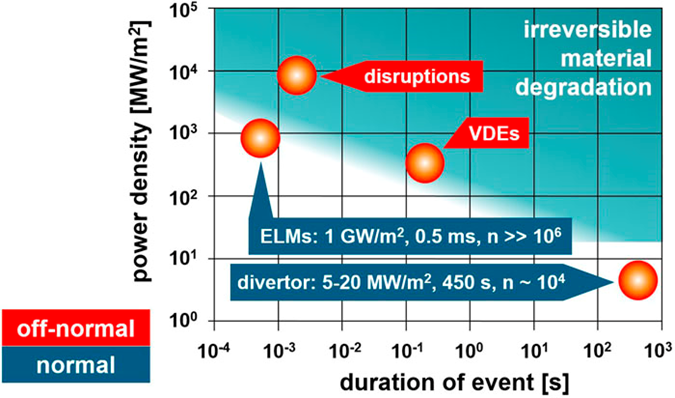
\includegraphics[scale=1]{Heat_loads_diagram.png}
    }
    \caption{Ожидаемые тепловые потоки, приходящие на ОПЭ в ИТЭР~\cite{Linke2019}. Бирюзова область соответствует области нанесения необратимого ущерба поверхности}\label{fig:ch1/Heat_loads_diagram}
\end{figure}

Значительную опасность представляют три типа событий: большие срывы тока, вертикальные смещения плазменного шнура и импульсно-периодические плазменные нагрузки во время ELM-событий. Большие срывы тока происходят при развитии глобальных магнитогидрониманических неустойчивостей. Они представляют наибольшую опасность, т.к. приводят к выбросу значительной части запасенной в плазме энергии на ОПЭ за времена порядка \SIrange{10}{100}{\milli\second}. Вертикальные смещения характерны для D-образного сечения плазменного шнура при утере устойчивости в вертикальном направлении за счет быстрых изменений параметров плазмы. События неконтролируемого вертикального смещения ведут к выходу за сепаратрису, создавая дополнительную тепловую нагрузку на ОПЭ за время порядка \SIrange{0.1}{1}{\second}. Возникновение импульсно-периодических плазменных нагрузок на ОПЭ характерно для плазменных разрядов в H-моде, переход в которую сопровождается формированием транспортного барьера на периферии плазмы. Образование транспортного барьера ведет к росту давления плазмы и его градиента на периферии пока не будет достигнут предел магнитогидрониманической устойчивости~\cite{Leonard2014}. Возникающая в результате неустойчивости (ELM-неустойчивости) вызывает быструю релаксацию давления с выбросом потока плазмы, содержащего порядка процента запасенной энергии в плазме, на ОПЭ за время \( \sim\SIrange{0.1}{1.0}{\milli\second} \). Согласно оценкам~\cite{Loarte2003, hender2007mhd, Pitts2017, Pitts2019}, потоки тепла во время переходных процессов в ИТЭР могут достигать $\sim\SI{10}{\giga\watt\per\meter\squared}$. Воздействие мощных плазменных потоков во время описанных переходных процессов может нанести серьезный ущерб поверхности (растрескивание, плавление, испарение и т.д.). Предотвращение возможного ущерба является приоритетной задачей, для решения которой разрабатываются соответствующие операционные системы и подходы~\cite{Lang2013,Evans2013,Lehnen2015}. Ввиду этого, далее в работе основное внимание будет уделено переходным процессам типа ELM-событий, последствия развития которых предполагаются либо допустимыми, либо могут быть минимизированы до приемлемого уровня.

Потоки частиц, приходящие на ОПЭ в действующих установках, в основном состоят из электронов, ионов и нейтралов перезарядки изотопов водорода. Возможно также наличие малой доли примеси более тяжелых атомов/ионов материалов ОПЭ, остаточного газа или примесей, вводимых в установку для кондиционирования стенок или распределения тепловых нагрузок. В проектируемых ТЯУ, в т.ч. и токамаке ИТЭР, корпускулярные нагрузки также будут включать продукты DT-реакции синтеза: высокоэнергетичные нейтроны (\SI{14.1}{\mega\electronvolt}) и альфа-частицы (\SI{3.5}{\mega\electronvolt}). Длительные режимы работы установок будут сопровождаться высокой дозой облучения ОПЭ, что также может приводить к модификации как поверхностной, так и объемной структуры. К тому же, важней задачей с точки зрения обеспечения радиационной безопасности является минимизация накопления радиоактивного трития в элементах установки на протяжении ее срока эксплуатации.

Плотность потока частиц на элементы первой стенки ИТЭР оценивается на уровне \SIrange{e18}{e20}{\particles\per\metre\squared\per\second}~\cite{DeTemmerman2021, Rivals2022}, когда для диверторных пластин "--- на уровне \SIrange{e23}{e24}{\particles\per\metre\squared\per\second}~\cite{Pitts2019,Orrico2023}, причем энергия приходящих ионов составляют величину порядка \SIrange{1}{100}{\electronvolt}. Оценка суммарной дозы облучения пластин дивертора в ИТЭР показывает, что за 5000 номинальных разрядов длительностью \SI{400}{\second} ее величина составит \( \sim \SIrange{e29}{e30}{\particles\per\metre\squared} \). Как показано на сравнительных диаграммах на рисунке~\cref{fig:ch1/fluxes_comparison}, условия эксплуатации ОПЭ в ИТЭР будут намного суровее, чем в действующих установках по исследованию магнитного удержания плазмы.
\begin{figure}[ht]
    \centerfloat{
        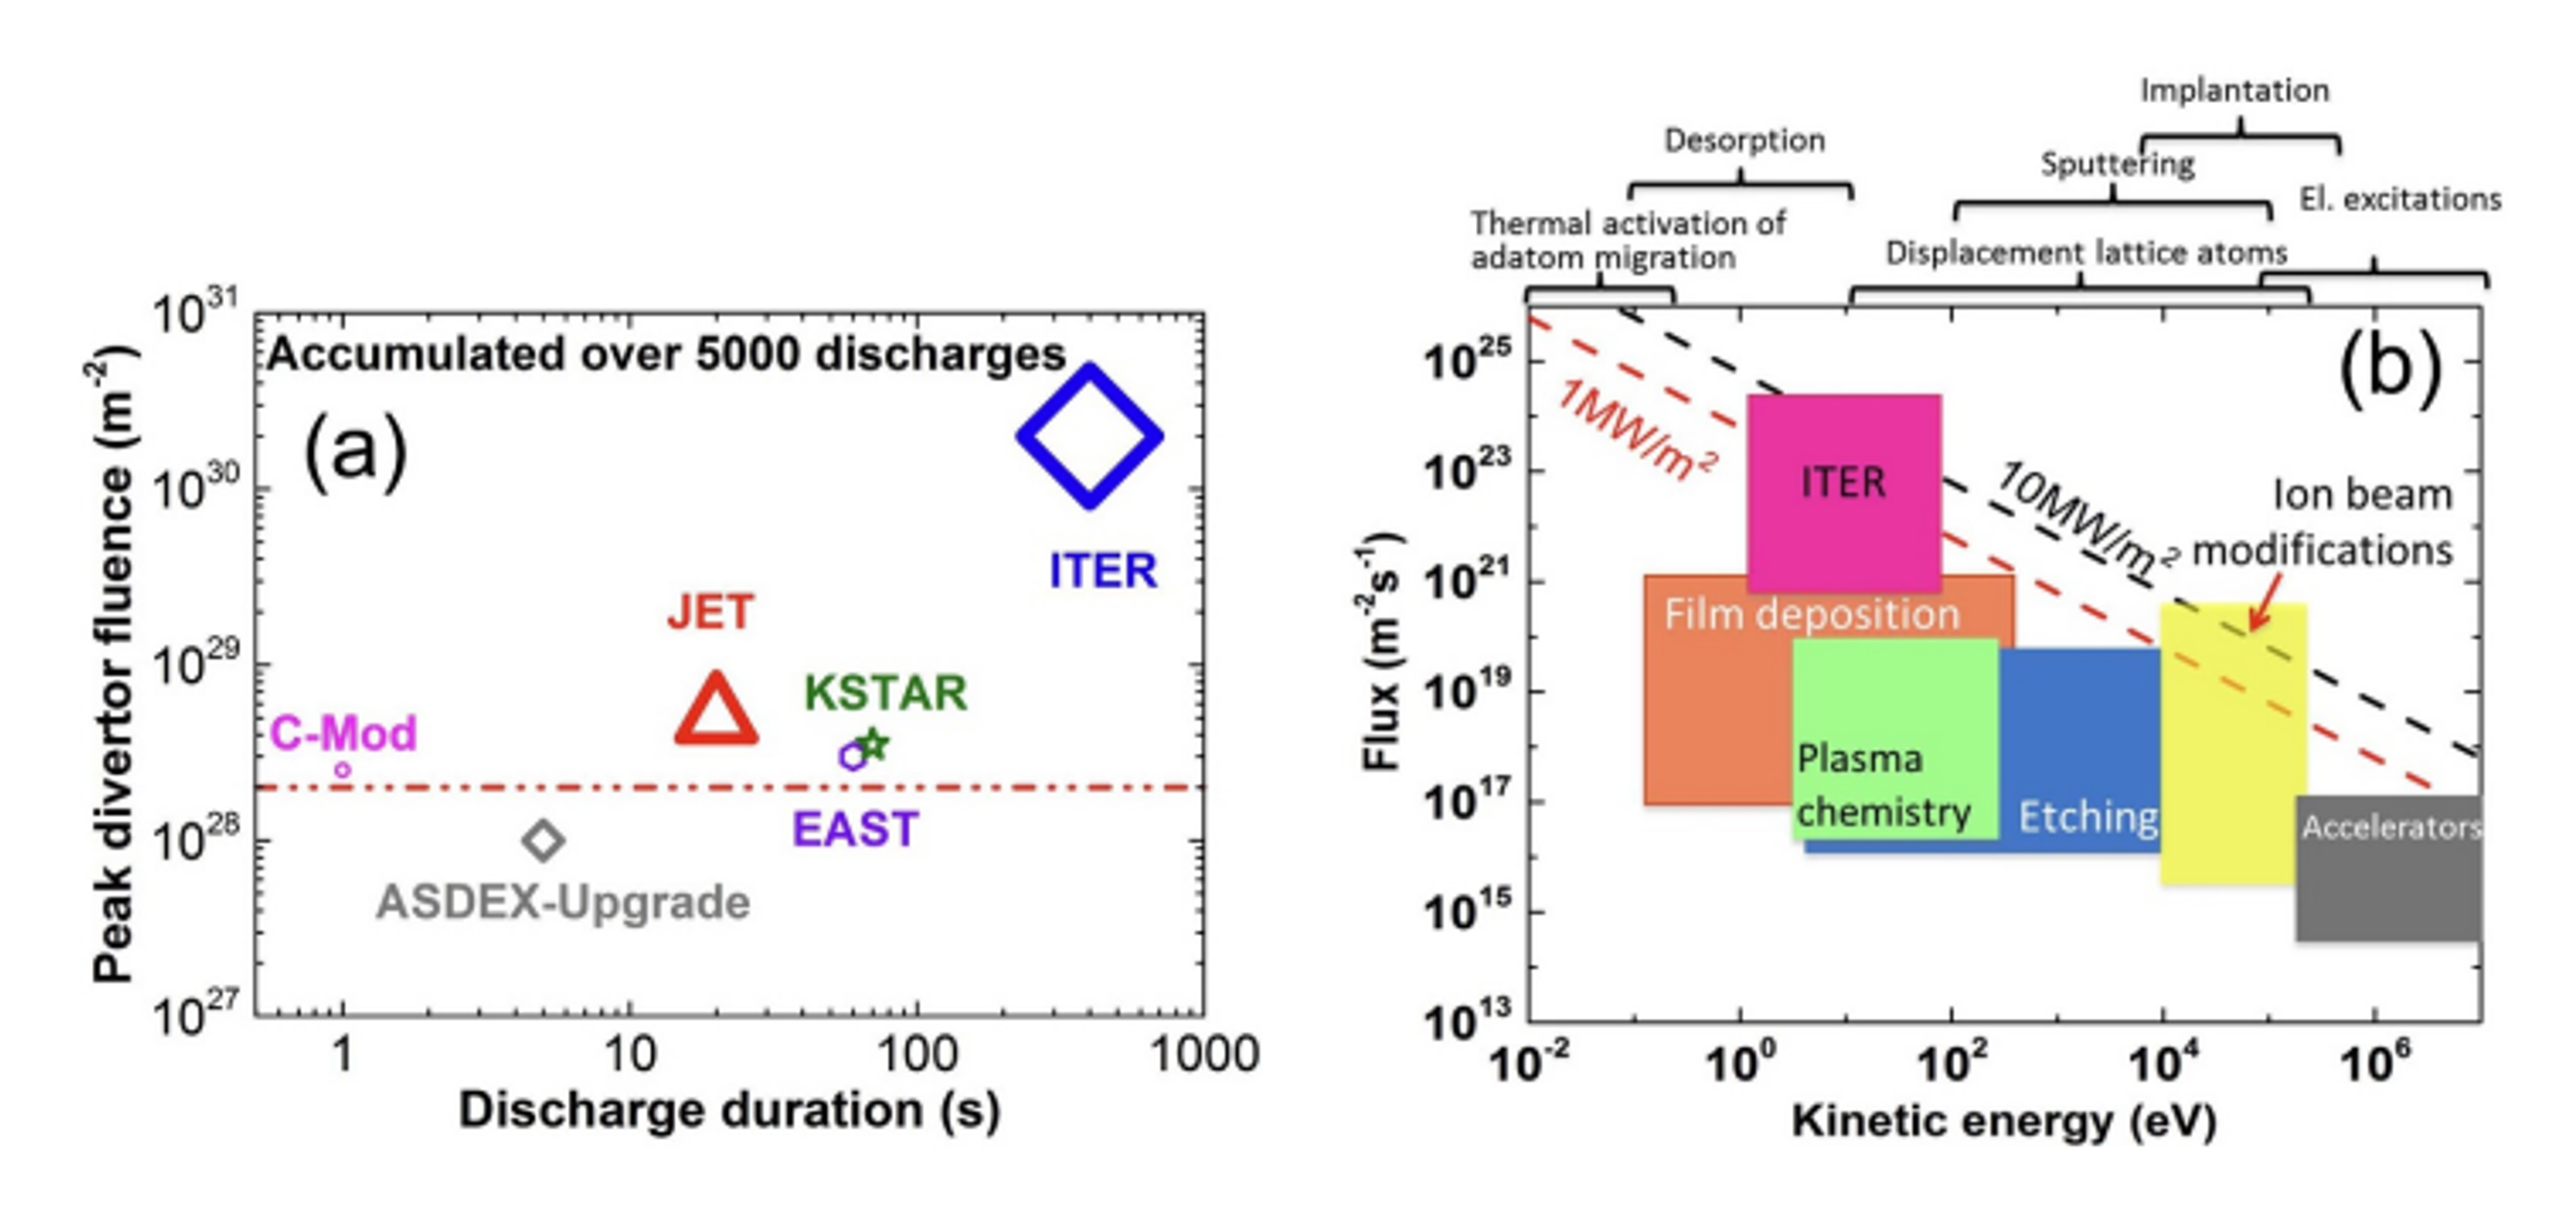
\includegraphics[scale=0.9]{fluxes_comparison.png}
    }
    \caption{Сравнение оцененной ионной дозы после 5000 тысяч нормальных плазменных разрядов в различных токамаках (слева) и характерных условий облучения в различных типах экспериментов~\cite{DeTemmerman2018}}\label{fig:ch1/fluxes_comparison}
\end{figure}
Энергии ионов в диверторе сопоставимы с энергиями, используемыми в различных методах плазменного осаждения и травления, однако плотности потока ионов и энергии на несколько порядков выше. Помимо этого, поток и энергия ионов, приходящих на поверхность ОПЭ, могут увеличиваться во время переходных процессов. Анализ данных с диагностических систем (зонды Ленгмюра и \(\mathrm{D}_\alpha\)-спектроскопия) токамака JET~\cite{Guillemaut2015,Guillemaut2018} демонстрирует кратное увеличение измерительных сигналов во время ELM-событий, что косвенно соответствуют пропорциональному росту потока частиц. Считается, что энергия частиц во время ELM-событий пропорциональна температуре плазмы на пьедестале~\cite{Eich2017}. При сохранении аналогичных зависимостей для токамака масштаба ИТЭР можно ожидать соответствующее превышение уровня стационарных нагрузок с энергия приходящих ионов порядка нескольких килоэлектронвольт.

Немаловажным остается влияние образования гелия и нейтронов на эксплуатацию ОПЭ. Генерируемы в ходе DT-реакции частицы гелия должны терять большую часть своей энергии в центре плазменного шнура, однако стационарное облучение материалов ионами гелия с низкой энергией также может оказывать существенное влияние. Известно, что облучение тугоплавких металлов ионами гелиевой плазмы индуцирует формирование гелиевых пузырей в объеме материала, а также может приводить к его структурным изменениям с образованием высокопостристых структур~\cite{Ueda2018,Kajita2018,Fedorovich2019}. Любые незапланированные структурные изменения морфологии поверхности ОПЭ будут влиять на процессы взаимодействия плазмы с ней, что может приводить к глобальным изменениям в режимах удержания плазмы.

Взаимодействие ионов с ОПЭ носит поверхностный характер. Падающий на поверхность поток частиц может приводить либо к обратной эмиссии частиц (отражение, распыление), либо к их имплантации. Средняя глубина внедрения частиц (за исключением эффектов каналирования) может достигать нескольких десятков нанометров в зависимости от состава и структуры мишени, сорта приходящих частиц и их энергии~\cite{eckstein2010penetration}. Ввиду гораздо большей глубины пробега нейтронов основные процессы взаимодействия происходят в объеме материалов. Облучение нейтронными потоками ведет к объемному нагреву материалов, их трансмутации, а также образованию дефектов кристаллической решетки за счет развития каскадов столкновений. Прогнозируемый уровень повреждений в конце срока службы токамака ИТЭР оценивается гораздо ниже инженерных ограничений~\cite{Villari2013}. Тем не менее, образование радиационных дефектов в материалах ОПЭ в ходе работы установки может влиять на удержание изотопов водорода.

\section{Материалы ОПЭ в ТЯУ}\label{sec:ch1/sec2}

Влияние описанных в предыдущим разделе отдельных типов нагрузок широко исследовалось в лабораторных условиях (исключением могут служить эффекты, связанные с облучением нейтронам с МэВ-ной энергии). В общем случае, они будут оказывать совместное влияние, что качественно проиллюстрировано на рисунке~\cref{fig:ch1/synergetic_diagram}. Синергетические эффекты воздействия на ОПЭ в не достижимых ранее условиях ТЯУ могут создавать новые вызовы для выбора их оптимальной конструкции.
\begin{figure}[ht]
    \centerfloat{
        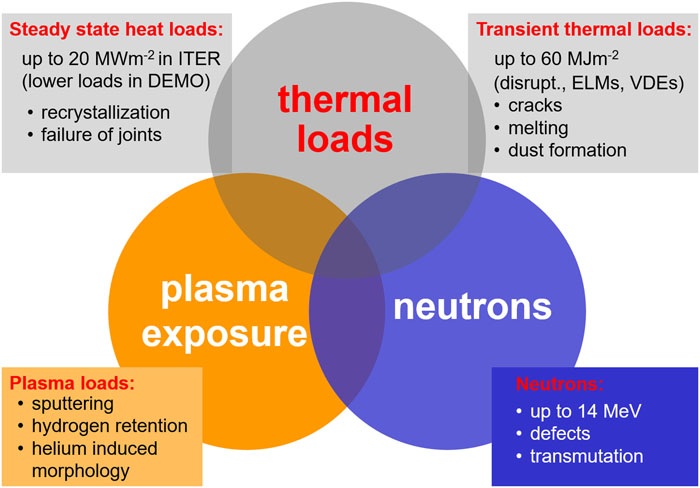
\includegraphics[scale=0.5]{synergetic_diagram.png}
    }
    \caption{Синергетические нагрузки и их основные последствия для ОПЭ при работе ТЯУ~\cite{Linke2019}}\label{fig:ch1/synergetic_diagram}
\end{figure}
Эти аспекты также накладывает совокупность требований и на выбор используемых материалов. К основным факторам, определяющим этот выбор, можно отнести термостойкость и теплопроводность, эрозионную устойчивость при ионном облучении, способность накапливать изотопов водорода, устойчивость и низкую активируемость при нейтронном облучении. Высокая термостойкость и теплопроводность, а также низкая эрозия при облучении легкими ионами характерны для тугоплавких металлов с большим зарядовым числом ядра ($Z$). Однако распыление и попадание в область горячей плазмы атомов таких материалов может приводить к увеличению потерь мощности на излучение из плазмы~\cite{Ptterich2019}. Более легкие материалы подвержены большей эрозии поверхности и могут влиять на динамику накопления изотопов водорода в ТЯУ. \nomenclature[P,00]{$Z$}{Атомный номер элемента}

Основными материалами, применяемыми в современных установках, являются графит (JT-60SA~\cite{Shirai2024}, T-15МД~\cite{Velikhov2024}), бериллий (JET~\cite{Maggi2024,Kappatou2025}), молибден(EAST~\cite{Gong2024}) и вольфрам (JET, EAST, WEST~\cite{Shi2025}, ASDEX-Upgrade~\cite{Rohde2009}). Углеродные материалы являются привлекательным выбором для ОПЭ ввиду ряда преимуществ. Проникновение углерода в плазму ведет к малым потерям мощности с излучением из-за его низкого зарядового числа ($Z=6$). Углеродные материалы характеризуются высокими теплостойкостью и значением теплопроводности ($\SIrange{100}{300}{\watt\per\meter\squared\per\kelvin}$ при комнатной температуре~\cite{Merola2004, Begrambekov2023}), сопоставимой с металлами. Помимо этого, нагрев поверхности до высоких температур (>\SI{3800}{\kelvin}) ведет к сублимации материала, а не плавлению, что предотвращает вероятность развития процессов взаимодействия расплава с приповерхностной плазмой и магнитным полем. Однако углеродные материалы более подвержены распылению при облучению легкими ионами, чем, например, вольфрам. а также характеризуются высоким коэффициентом химического распыления при облучении изотопами водорода. Для сравнения на рисунке~\cref{fig:ch1/sputerring_yields} приведены расчетные коэффициенты распыления углерода (физического и химического), бериллия и вольфрама. Влияние химического распыления может быть минимизировано обеспечением <<благоприятного>> режима облучения, но другим важным недостатком углеродных материалов является накопление изотопов водорода. Изотопы водорода образуют прочные C-H связи, что может приводить к чрезмерному накоплению трития в переосажденных пленках и затруднять извлечению трития из установки~\cite{Gasparyan2024}. Помимо этого, интенсивное облучение потоками нейтронов и компонентов плазмы может приводить к деградации теплофизических свойств~\cite{Wu1994} и структурным изменениям поверхностных слоев~\cite{Wang2018,Begrambekov2019,Seyedhabashi2025}.

\begin{figure}[ht]
    \centerfloat{
        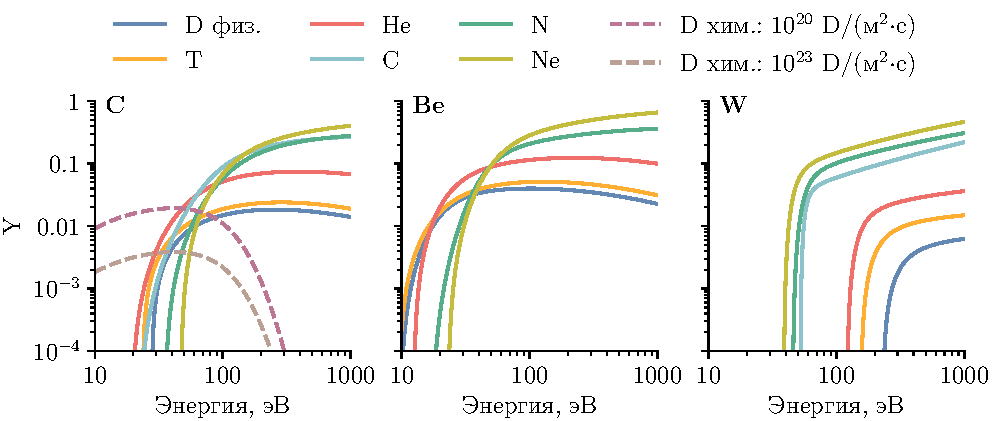
\includegraphics[scale=1]{sputerring_yields.pdf}
    }
    \caption{Расчетные зависимости коэффициентов физического распыления бериллия, углерода и вольфрама от энергии некоторых типов ионов при нормальном падении~\cite{international2001iaea, behrisch_2025}. Для углерода также приведены зависимости коэффициента химического распыления дейтерием при комнатной температуре и различных значениях потока~\cite{Roth1999,Roth2004}}\label{fig:ch1/sputerring_yields}
\end{figure}

Бериллий, как и углерод, обладает низким атомным номером ($Z=4$), что обеспечивает относительно хорошую совместимость за счет минимизации потерь мощности на излучения при проникновение бериллия в область горячей плазмы. Он также обладает высокой теплопроводностью (\SI{200}{\watt\per\meter\per\K}) и относительно высокой температурой плавления (\SI{1560}{\kelvin})~\cite{Ho1974}. По сравнению с углеродными материалами, скорость химического распыления~\cite{Brezinsek2014} и накопления изотопов водорода~\cite{DeTemmerman2021} в нем существенно меньше. Переход к металлической облицовке в токамаке JET привел к снижению интегральной эрозии ОПЭ и, как следствие, накоплению изотопов водорода~\cite{Brezinsek2015}. Бериллий также химически активен, что позволяет эффективно связывать кислород. Не смотря на явные преимущества бериллия как материала для ОПЭ, он обладает рядом существенных недостатков. Первым из них является токсичность бериллиевой пыли, что требует применения специальных мер по работе с ним~\cite{Strupp2011}. Вторым недостатком является низкая энергия связи атомов кристаллической решетки, что приводит к более высокому коэффициенту физического распыления по сравнению с графитом (рис.~\cref{fig:ch1/sputerring_yields}) и, соответственно, меньшему сроку службы под действием интенсивного ионного облучения. Следующим негативным свойством является деградация теплофизических свойств и охрупчивание бериллия, являющееся синергетическим эффектом облучения потоками нейтронов и гелия~\cite{Kesternich2003,Gilbert2012}. Последним является малая температура плавления по сравнению с иными материалами, что ограничивает использование бериллия в высоконагруженных областях установки без активного охлаждения. Совокупность этих и иных особенностей послужили причиной принятия решения об отказе от использования бериллия в качестве ОПЭ токамака ИТЭР~\cite{Barabaschi2025}, однако использование бериллия рассматривается для российского токамака ТРТ~\cite{Mazul2021,Piskarev2024}.

Молибден ($Z=42$) и вольфрам ($Z=74$) являются тугоплавкими металлами с высокими температурами плавления: \SI{2896}{\kelvin} и \SI{3695}{\kelvin}, соответственно. Однако вольфрам предпочтительнее по причине более высоких эксплуатационных характеристик, хоть и обладает рядом свойств усложняющих технологическое производство элементов облицовки с ним~\cite{Piskarev2024}. Исходя из этого, основное внимание будет уделено вольфраму. Помимо высокой теплостойкости, вольфрам характеризуется низким коэффициентом распыления легкими ионами (рис.~\cref{fig:ch1/sputerring_yields}), совместимостью с нейтронным облучением и низкой растворимостью изотопов водорода~\cite{Pintsuk2012,Rieth2019}. Явным недостатком вольфрама является вероятность распыления тяжелыми примесными ионами в плазме или ее легкими основными компонентами с высокой энергией, сопровождаемое загрязнением плазмы частицам с высоким атомным номером. Как отмечалось в разделе~\cref{sec:ch1/sec1}, потоки частиц плазмы с высокой энергией ожидаются в ходе различных переходных процессов. Известна также проблема образования трещин на поверхности вольфрама при циклических тепловых нагрузках, характерных для ELM-событий. Дополнительно необходимо отметить активно исследуемые в последнее время изменения поверхности вольфрама при облучении ионами гелиевой плазмы. В условиях, характерных для диверторной области токамаков, облучение ионами гелия ведет к формированию высокопористой наноструктуризованной морфологии, называемой <<пух>>~\cite{Ueda2018,Kajita2018,Fedorovich2019,hammond2017helium,Kajita2020,Wright2022}. Рост вольфрамового <<пуха>> на поверхности может повысить вероятность зажигания униполярных дуг с соответствующем увеличением уровня эрозии поверхности. Невзирая на недостатки вольфрама, он выбран в качестве основного материала ОПЭ для ИТЭР~\cite{Pitts2025} и находится в приоритетном списке как для ТРТ~\cite{Piskarev2024}, так и для других установок, проектируемых в настоящее время.


Учитывая риски появления тяжелой примеси в горячей плазме при распылении вольфрама, рассматривается применения различных материалов для нанесения кондиционирующих покрытий. Двумя распространенными материалами, применяемыми в действующих установках, являются литий ($Z=5$) и бор ($Z=3$). Оба материала обладают низким атомным номером и являются химически активными по отношению к кислороду и углероду, что позволяет снизить долю более тяжелой примеси в плазме~\cite{Winter1996,Wauters2020}. С другой стороны, более высокая скорость эрозии покрытий требует применения методов их регулярного обновления. Тем не менее, эксперименты на токамаках ASDEX-Upgrade~\cite{Krieger2023} и EAST~\cite{Yu2023} продемонстрировали, что применении легких материалов для кондиционирования стенок может обеспечить режимы плазменных разрядов с низким рециклингом изотопов водорода, что может привести к осуществлению длительных стабильных разрядов~\cite{Zakharov2019}. Помимо методов нанесения защитных покрытий, ведется активное развитие альтернативных вариантов, например самопассивируемые сплавы вольфрама с пониженным термоокислением~\cite{Litnovsky2020} и капиллярно-пористые системы с жидкими металлами~\cite{Lublinskii2015}, которые, возможно, решат проблемы, характерные для традиционных материалов.

\section{Накопление изотопов водорода в вольфраме}

Как показно в предыдущем разделе, вольфрам обладает совокупностью свойств, определяющим его применимость в качестве материала ОПЭ. Перспектива его использования инициировала всестороннее изучение закономерностей накопления изотопов водорода в условиях, ожидаемых в ТЯУ. Необходимость детального анализа во многом обусловлена необходимостью контроля за содержанием радиоактивного трития. Так, для токамака ИТЭР установлен административный лимит в \SI{700}{\gram} по интегральному накоплению в элементах вакуумной камеры с учетом возможных погрешностей и накопления в крионасосах~\cite{Roth1}. В данном разделе приведены основные механизмы и экспериментальные результаты исследования накопления изотопов водорода в вольфраме.

\subsection{Механизмы накопление изотопов водорода в ТЯУ}

Изотопы водорода могут накапливаться на поверхности ОПЭ за счет адсорбции низкоэнергетичных атомов или молекул. Совокупность каналов адсорбции является процессом динамического (краткосрочного) удержания и не представляет особой проблемы, т.к. дегазация поверхности протекает достаточно быстро при повышенных температурах. Выделяют два основных канала долгосрочного удержания изотопов водорода: захват в объеме материала и соосаждение~\cite{Gasparyan2024, Skinner2009}. Также можно отметить накопление изотопов на поверхности или в объеме пылевых микрочастиц, образующихся в процессе эрозии поверхностных слоев ОПЭ. Накопление в пылевых частицах сильно зависит от механизма их образования и во многом может описываться процессами, определяющими захват водорода в объеме ОПЭ или при соосаждении. В силу этого, основное внимание будет уделено двум другим процессам долгосрочного удержания изотопов водорода в ТЯУ.

Основные процессы, определяющие долгосрочное накопление, схематически представлены на рисунке~\cref{fig:ch1/retention_mechanisms}.
\begin{figure}[ht]
    \centerfloat{
        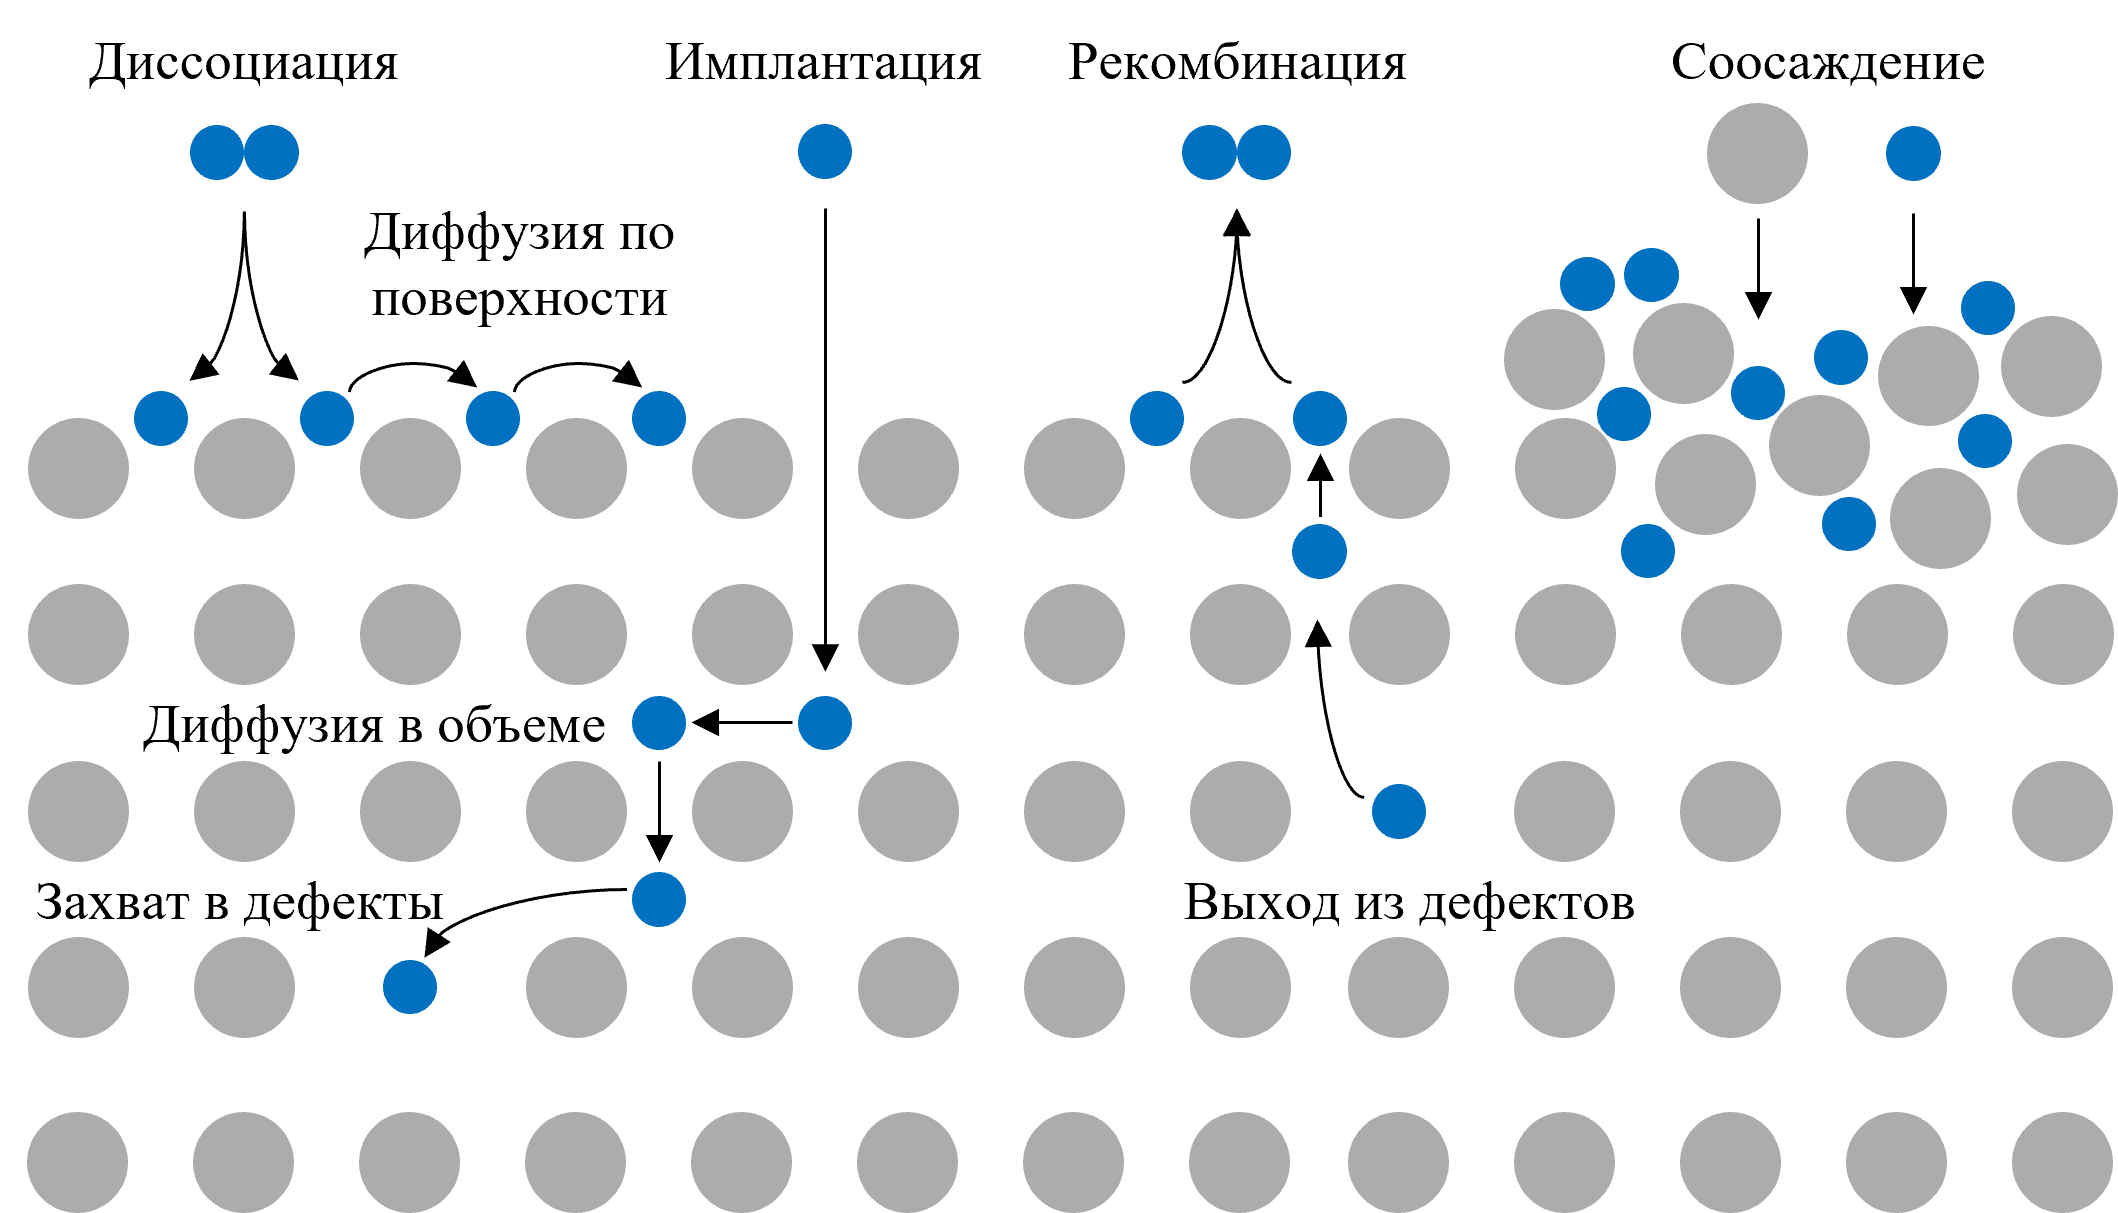
\includegraphics[scale=1]{retention_mechanisms.png}
    }
    \caption{Схематическое представление процессов захвата изотопов водорода при имплантации и соосаждении. Синие круги соответствуют атомам водорода, серые "--- атомам облучаемого материала}\label{fig:ch1/retention_mechanisms}
\end{figure}
Захват изотопов водорода при ионном облучении изначально происходит за счет имплантации частиц. Вероятность внедрения ионов определяется интегральным коэффициентом отражения, зависящим от параметров облучения и сортов взаимодействующих частиц. При попадании в объем внедренные частицы продолжают движение, теряя свою начальную энергию за счет упругих и неупругих потерь, пока не термализуются. Подвижность атомов водорода в металлах, как вольфрам, остается достаточно высокой при повышенных температурах, что позволяет им диффундировать обратно к поверхности и десорбироваться за счет различных процессов, например рекомбинации. С другой стороны, характерная глубина внедрения ионов в условиях токамака не превышает десятков нанометров. Интенсивное облучение поверхности приводит к быстрому насыщению водорода в зоне имплантации, что инициирует распространение водорода вглубь материала. В ходе диффузии подвижные атомы водорода могут захватываться различными дефектами кристаллической решетки, представляющие собой более глубокие потенциальные ямы по сравнению с межузельными положениями. Учитывая диффузионный характер накопления, величина интегрального накопления пропорциональна квадратному корню из времени (дозы) облучения, что наблюдается в многочисленных экспериментах~\cite{Ogorodnikova2003,Ogorodnikova2009,Sugiyama2014,Zhang2020}. Ввиду малой растворимости водорода в вольфраме, долгосрочное накопление будет определяться распределением и концентрацией дефектов, образование которых будет происходить при ионном и нейтронном облучении.

Процесс соосаждения водорода и материалов первой стенки в токамаках происходит в несколько итерационных этапов. Непрерывное распыление материалов ОПЭ приводит к попаданию примесных атомов в плазму, в которой они ионизуются. Ионы материалов стенки за счет процессов переноса в пристеночной плазме в итоге нейтрализуются и осаждаются на других элементах облицовки, инициируя рост поверхностных пленок. В то же время осаждаемые пленки подвергаются непрерывному облучению потоками частиц из плазмы. Совместное протекание обоих процессов ведет к практическому равномерному накоплению изотопов водорода, интегральная величина которого растет приблизительно линейно с временем. Важно заметить, что накопление изотопов водорода в процессе совместного соосаждения также сопровождается всеми процессами, характерными при имплантации в объем.

Результаты, полученные на современных токамаках, указывают на то, что соосаждение является доминирующим каналом накопления изотопов водорода. Параметры удержания водорода, физические свойства и скорость роста пленок сильно зависят от параметров совместного осаждения~\cite{Gasparyan2019,Krat2020,Krat2025}. Доля водорода в пленках может достигать десятков процентов для различных материалов (см. Рисунок~\cref{fig:ch1/codeposition_review}).
\begin{figure}[ht]
    \centerfloat{
        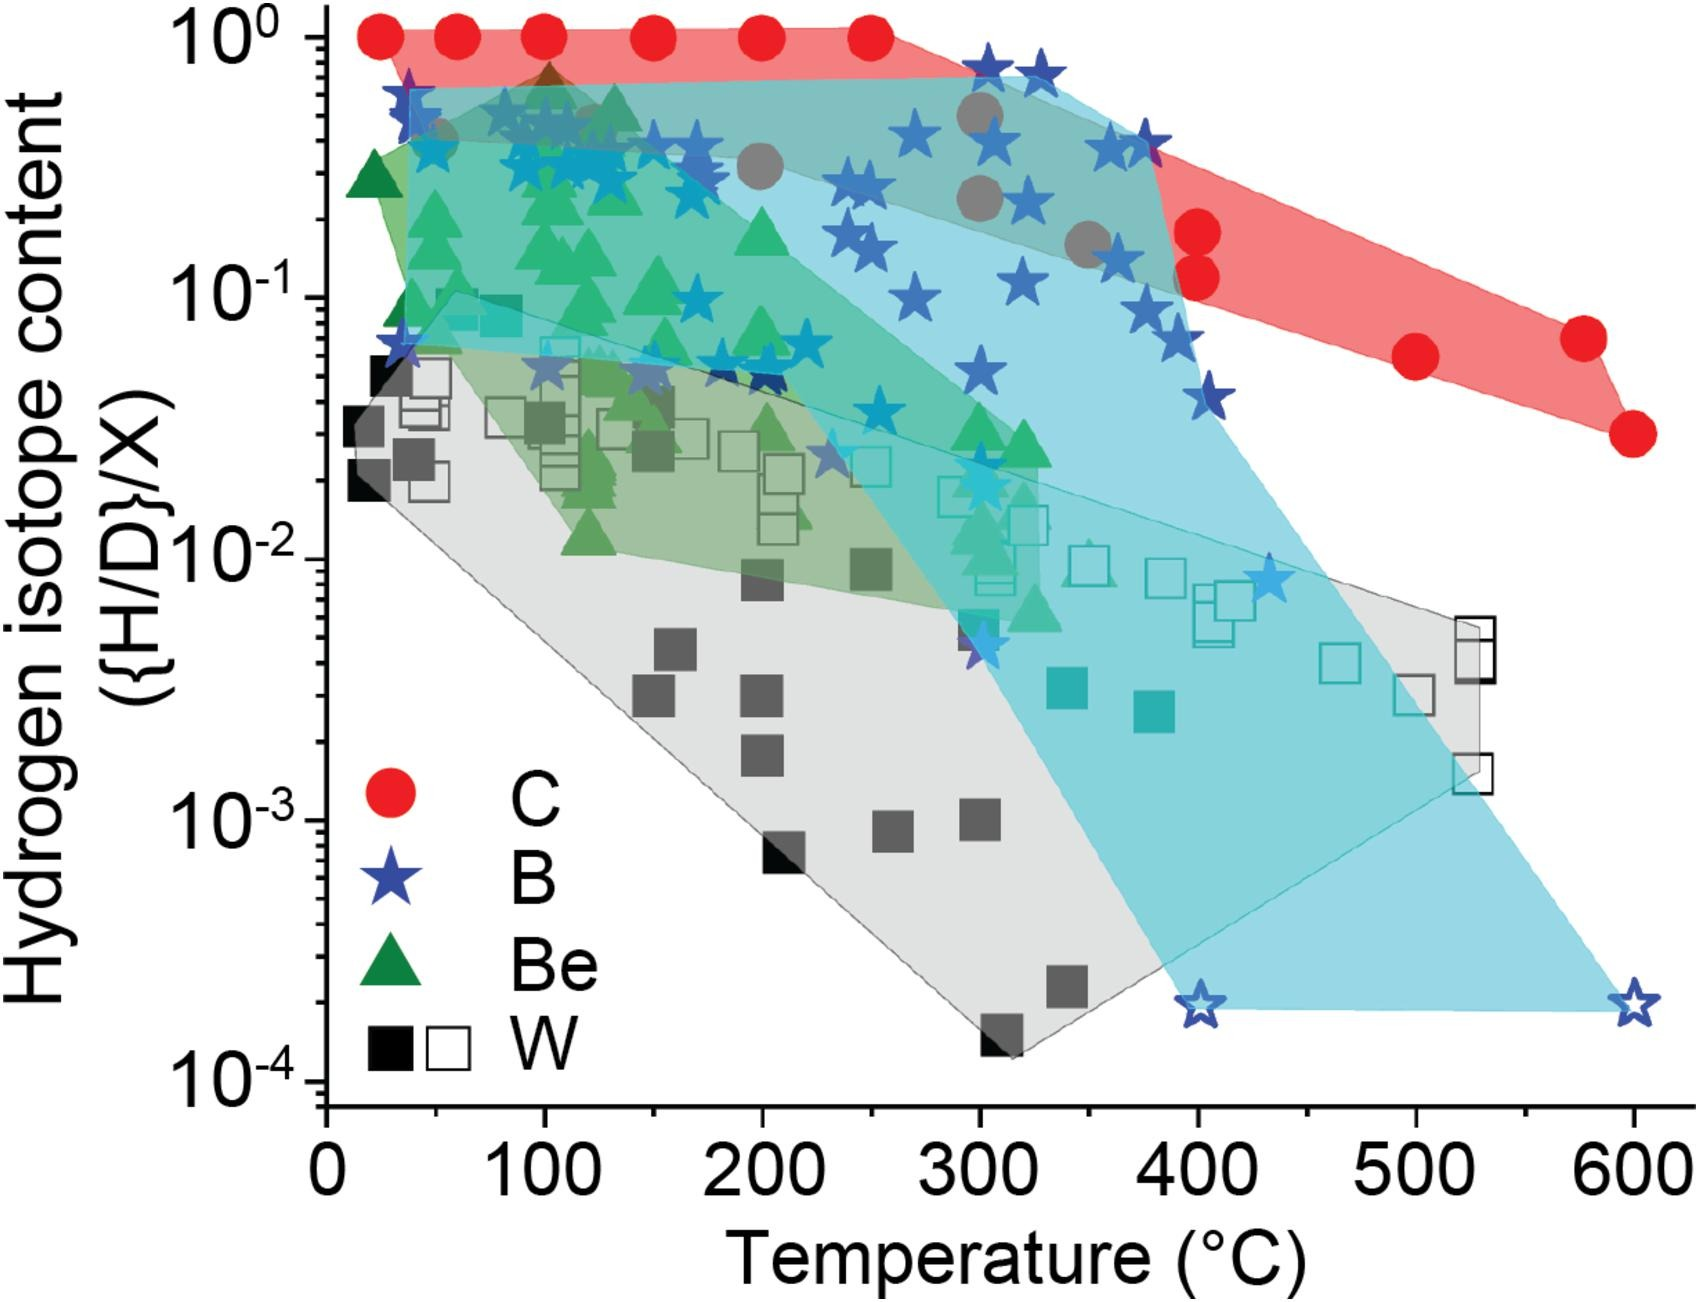
\includegraphics[scale=0.15]{codeposition_review.png}
    }
    \caption{Содержание изотопов водорода в зависимости от температуры совместного осаждения для пленок бора (голубая область), вольфрама (серая область), бериллия (зеленая область) и углерода (красная область)~\cite{Pitts2025}}\label{fig:ch1/codeposition_review}
\end{figure}
Примечательно, что содержание водорода оказывается систематически меньше в пленках вольфрама по сравнению с другими материалами. Помимо этого, скорость образования вольфрамовых пленок может быть меньше в ТЯУ из-за более высокого порога распыления. Однако недавний \textit{post-mortem} анализ образцов-свидетелей из токамака WEST указывает на образование переосажденных слоев с толщиной несколько микрометров~\cite{Bucalossi2024}.

\subsection{Взаимодействие изотопов водорода с вольфрамом}

Транспорт внедренных атомов водорода в вольфраме включает множество механизмов, которые можно разделить на несколько групп: диффузионные механизмы, взаимодействие с различными типами дефектов и поверхностные процессы. Качественное описание каждой из групп можно дать на основе одномерного представления пространственного распределения потенциальной энергии атомов водорода вблизи поверхности материала (см. рисунок~\cref{fig:ch1/potential_diagram_all}). Важно заметить, что в реальности ситуация оказывается гораздо сложнее, а распределение энергии водорода в материале с дефектами кристаллической решетки представляет из себя трехмерное пространство с совокупностью локальных экстремумов и седловых точек. Получение детальной информации о распределении потенциальной энергии возможно при помощи \textit{ab initio} методов, как теория функционала электронной плотности (DFT).

\nomenclature[A, 7]{DFT}{Теория функционала электронной плотности (Density functional theory)}

\begin{figure}[ht]
    \centerfloat{
        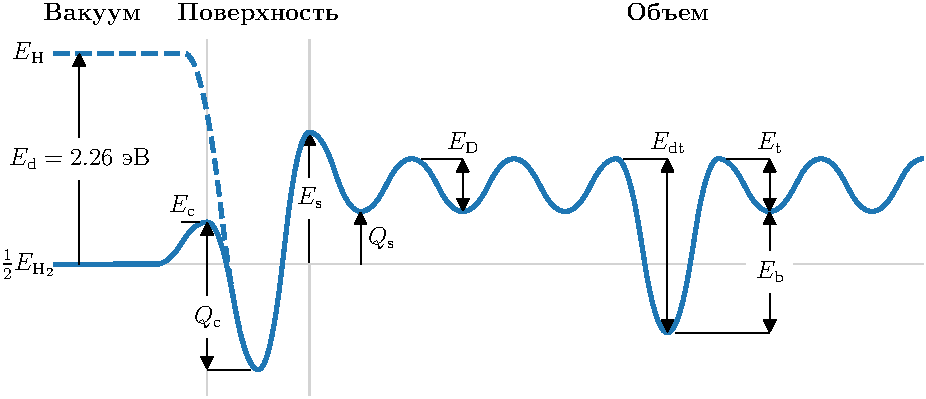
\includegraphics[scale=1]{potential_diagram_all.pdf}
    }
    \caption{Схематическая диаграмма потенциальной энергии водорода вблизи поверхности металла с положительной теплотой растворения. Уровни энергии отсчитываются от связанного состояния атома в молекуле водорода, расположенной далеко в вакууме}\label{fig:ch1/potential_diagram_all}
\end{figure}

\subsubsection{Диффузия}

Отталкивающий характер взаимодействия между атомами кристаллической решетки и водорода определяет предпочтительная оккупация последним межузульных положений, являющимися локальными минимумами потенциальной энергии. Для вольфрама с объемно-центрированной кубической решеткой наиболее устойчивыми положениями являются тетраэдрическое и октаэдрическое, причем первое является более энергетически выгодным со значение теплоты растворения $Q_\mathrm{c}$\nomenclature[P, 01]{$Q_\mathrm{s}$}{Теплота растворения [\si{\electronvolt}]} равным \SIrange{0.9}{1.0}{\electronvolt}~\cite{Heinola2010,Fernandez2015,Zhou2024}. В процессе колебаний атомы водорода могут перескакивать между равновесными положениями, распространясь стохастически по объему материала. Направления диффузионный поток атомов водорода $\mathbf{J}$ может быть обусловлен градиентами химического потенциала с вкладом $\mathbf{J}_c$ и температуры с вкладом $\mathbf{J}_T$~\cite{Longhurst1985, Krom1999, Martinez2021}:
\begin{equation}
    \mathbf{J}=\mathbf{J}_c+\mathbf{J}_T.
\end{equation}
В приближении малой концентрации растворенного водорода и отсутствия градиента напряжений в решетке вольфрама вклад от градиента химического потенциала можно редуцировать к влиянию градиента концентрации (закон Фика), определяющего поток $\mathbf{J}_{c}$:
\begin{equation}
    \mathbf{J}_{c} = -D \nabla \cm,
\end{equation}
где $D$ [\si{\meter\squared\per\second}] "--- коэффициент диффузии, $\cm$ [\si{\atoms\per\meter\cubed}] "--- концентрация атомов подвижного водорода. Диффузия, вызванная градиентом концентрации, является термоактивируемым процессом и в обычных условиях протекает быстрее с ростом температуры. Температурная зависимость коэффициента диффузии обычно описывается в соответствии с законом Аррениуса:
\begin{equation}
    D=D_0 \exp\left( -\frac{E_\mathrm{D}}{k_\mathrm{B}T} \right),
\end{equation}
где $E_\mathrm{D}$ [\si{\electronvolt}] "--- энергия активации диффузии, $k_\mathrm{B}=\SI{8.617e-5}{eV\per\kelvin}$ "--- постоянная Больцмана, $T$ [\si{\kelvin}] "--- абсолютная температура.

\nomenclature[P, 02]{$J$}{Поток атомов [\si{\atoms\per\meter\squared\per\second}]}
\nomenclature[P, 03]{$J_{c}$}{Поток атомов, индуцированный градиентом концентрации [\si{\atoms\per\meter\squared\per\second}]}
\nomenclature[P, 04]{$J_{T}$}{Поток атомов, индуцированный градиентом температуры (\si{\atoms\per\meter\squared\per\second})}
\nomenclature[P, 05]{$D$}{Коэффициент диффузии [\si{\meter\squared\per\second}]}
\nomenclature[P, 06]{$\cm$}{Концентрация подвижного водорода [\si{\atoms\per\meter\cubed}]}
\nomenclature[P, 07]{$E_\mathrm{D}$}{Энергия активация диффузии" [\si{\electronvolt}]}
\nomenclature[P, 08]{$k_\mathrm{B}$}{Постоянная Больцмана [\si{\electronvolt\per\kelvin}]}
\nomenclature[P, 09]{$T$}{Абсолютная температура [\si{\kelvin}]}

Определение коэффициента диффузии проводилось как посредством экспериментов, так и путем моделирования. Параметры коэффициента диффузии, определенные \textit{Р. Фраунфельдером} ($D_0=\SI{4.1e-7}{\metre\squared\per\second}$, $E_\mathrm{D}=\SI{0.39}{\electronvolt}$, $T=\SIrange{1100}{2400}{K}$)~\cite{frauenfelder1969solution}, продолжительное время считались наиболее надежными. Последующие результаты моделирования методом DFT~\cite{Heinola2010,Fernandez2015,Zhou2024} и недавние эксперименты~\cite{Holzner2020} указывают на большую подвижность атомов водорода в вольфраме с энергией активации диффузии в диапазоне \SIrange{0.2}{0.28}{\electronvolt}. Указанный диапазон согласуется с результатами Фраунфельдера при учете экспериментальных данных в высокотемпературной области, когда влиянием центров захвата на диффузию можно пренебречь~\cite{Heinola2010}. Тем не менее, значения коэффициента диффузии изотопов водорода сильно варьируются в литературе~\cite{remi_delaporte_mathurin_2024_13912922}, что значительно затрудняет проведение оценок накопления в материалах ОПЭ.

Облучение ОПЭ мощными тепловыми потоками неминуемо приведет к образованию температурных градиентов. Такая ситуация особо актуальна для конструкций элементов с активным водяным охлаждением, как диверторные моноблоки токамака ИТЭР. Градиент температур индуцирует поток термодиффузии $\mathbf{J}_T$ (эффект Соре):
\begin{equation}
    \mathbf{J}_{T} = -D\frac{\cm Q^*}{kT^2} \nabla T,
\end{equation}
направление которого определяется знаком теплоты переноса $Q^*$ [\si{\electronvolt}].
\nomenclature[P, 10]{$Q^*$}{Теплота переноса [\si{\electronvolt}]}

К сожалению, в настоящее время отсутствует общепринятое значение теплоты транспорта водорода в вольфраме. Экспериментальные измерения показывают, что теплота переноса в металлах с положительной теплотой растворения отрицательна и незначительно растет с температурой~\cite{Longhurst1985}. Оценки величины методом молекулярной динамики~\cite{Martinez2021,Dasgupta2023} также подтверждают отрицательное значение, но определенная функциональная зависимость обратно пропорционально квадрату температуры:
\begin{equation}
    \label{eq:ch1/heat_transport}
    Q^*=-0.0045 \kB T^2.
\end{equation}

\subsubsection{Центры захвата}

Дефекты в кристаллической решетке вольфрама, такие как вакансии, примеси, дислокации или пустоты, создают потенциальные энергетические ямы, более глубокие, чем для междоузлий. Такие дефекты являются потенциальными <<ловушками>> для подвижных атомов водорода. Захваченные в ловушки атомы становится <<иммобильным>> и могут покинуть ее, если тепловой энергии достаточно для преодоления потенциального барьера $E_\mathrm{dt}$ [\si{\electronvolt}]. Упрощенный процесс захвата можно представить в следующем виде~\cite{Drexler2020}:

\begin{equation*}
    \underset{\text{дефект}}{[\quad]} + \underset{\text{междоузлие}}{(\mathrm{H})} \mathop{\longleftrightarrows}^{\nu_\mathrm{t}}_{\nu_\mathrm{dt}}  \underset{\text{дефект}}{[\mathrm{H}]} +  \underset{\text{междоузлие}}{(\quad)},
\end{equation*}
где \( \nu_\mathrm{t} \) [\si{\metre\cubed\per\second}] и \( \nu_\mathrm{dt}\) [\si{\per\second}] скорости захвата и выхода из дефекта. Скорости обоих процессов определяются законом Аррениуса:
\begin{subequations}
    \begin{align}
        \nu_\mathrm{t} & = \nu_{\mathrm{t},0} \exp \left( -\frac{E_\mathrm{t}}{\kB T} \right); \\
        \nu_\mathrm{dt} & = \nu_{\mathrm{dt},0} \exp  \left( -\frac{E_\mathrm{dt}}{\kB T} \right),
    \end{align}
\end{subequations}
где \( E_\mathrm{t} \) [\si{\electronvolt}] "--- энергия активация захвата в дефект. Обычно полагается, что скорость захвата определяется диффузией: \( E_\mathrm{t} \approx E_\mathrm{D} \).

\nomenclature[P, 11]{\( \nu_\mathrm{t} \)}{Скорость захвата атомов в дефекты [\si{\metre\cubed\per\second}]}
\nomenclature[P, 12]{\( \nu_\mathrm{dt} \)}{Скорость выхода атомов из дефектов  [\si{\per\second}]}
\nomenclature[P, 13]{\( E_\mathrm{t} \)}{Энергия активация захвата в дефект [\si{\electronvolt}]}
\nomenclature[P, 14]{\( E_\mathrm{dt} \)}{Энергия активации выхода из дефекта}

Информацию о параметрах центров захвата можно получить экспериментально или путем моделирования. Моделирование позволяет рассчитать энергию связи атома с дефектом \( E_\mathrm{b} \), когда рамках экспериментов наиболее надежно определяют барьер выхода из ловушек \( E_\mathrm{dt}=E_\mathrm{} \). Широко распространенным методом определения параметров дефектов является термодесорбционная спектроскопия (ТДС). Энергия связи зависит от типа дефекта. Исчерпывающие обзоры ~\cite{Ogorodnikova2015,Persianova2024}

Дефекты в материале можно классифицировать на два типа. Первый тип, часто называемый внутренними дефектами (или естественными дефектами), является свойственным материалу, такими как примеси и границы зерен. Второй тип, внешние дефекты, возникают в результате внешних воздействий, включая повреждения от бомбардировки частицами (такими как ионы и нейтроны) или механического напряжения, и могут развиваться во времени и пространстве.


Внешние дефекты имеют решающее значение для характеристики термоядерных реакторов из-за высоких потоков нейтронов, с которыми компоненты, находящиеся поблизости от плазмы, вероятно, будут взаимодействовать. Интенсивная бомбардировка нейтронами в этих условиях может привести к значительным повреждениям, создавая высокую плотность внешних дефектов, которые могут повлиять на свойства и работу материала. Понимание формирования и эволюции этих дефектов имеет важное значение для прогнозирования срока службы и надежности компонентов реактора. Несмотря на их важность, динамика формирования внешних ловушек в результате взаимодействия с нейтронами не была широко исследована в литературе.

\nomenclature[A, 8]{ТДС}{Термодесорбционная спектроскопия}

\subsubsection{Поверхностные процессы}

\begin{figure}[ht]
    \centerfloat{
        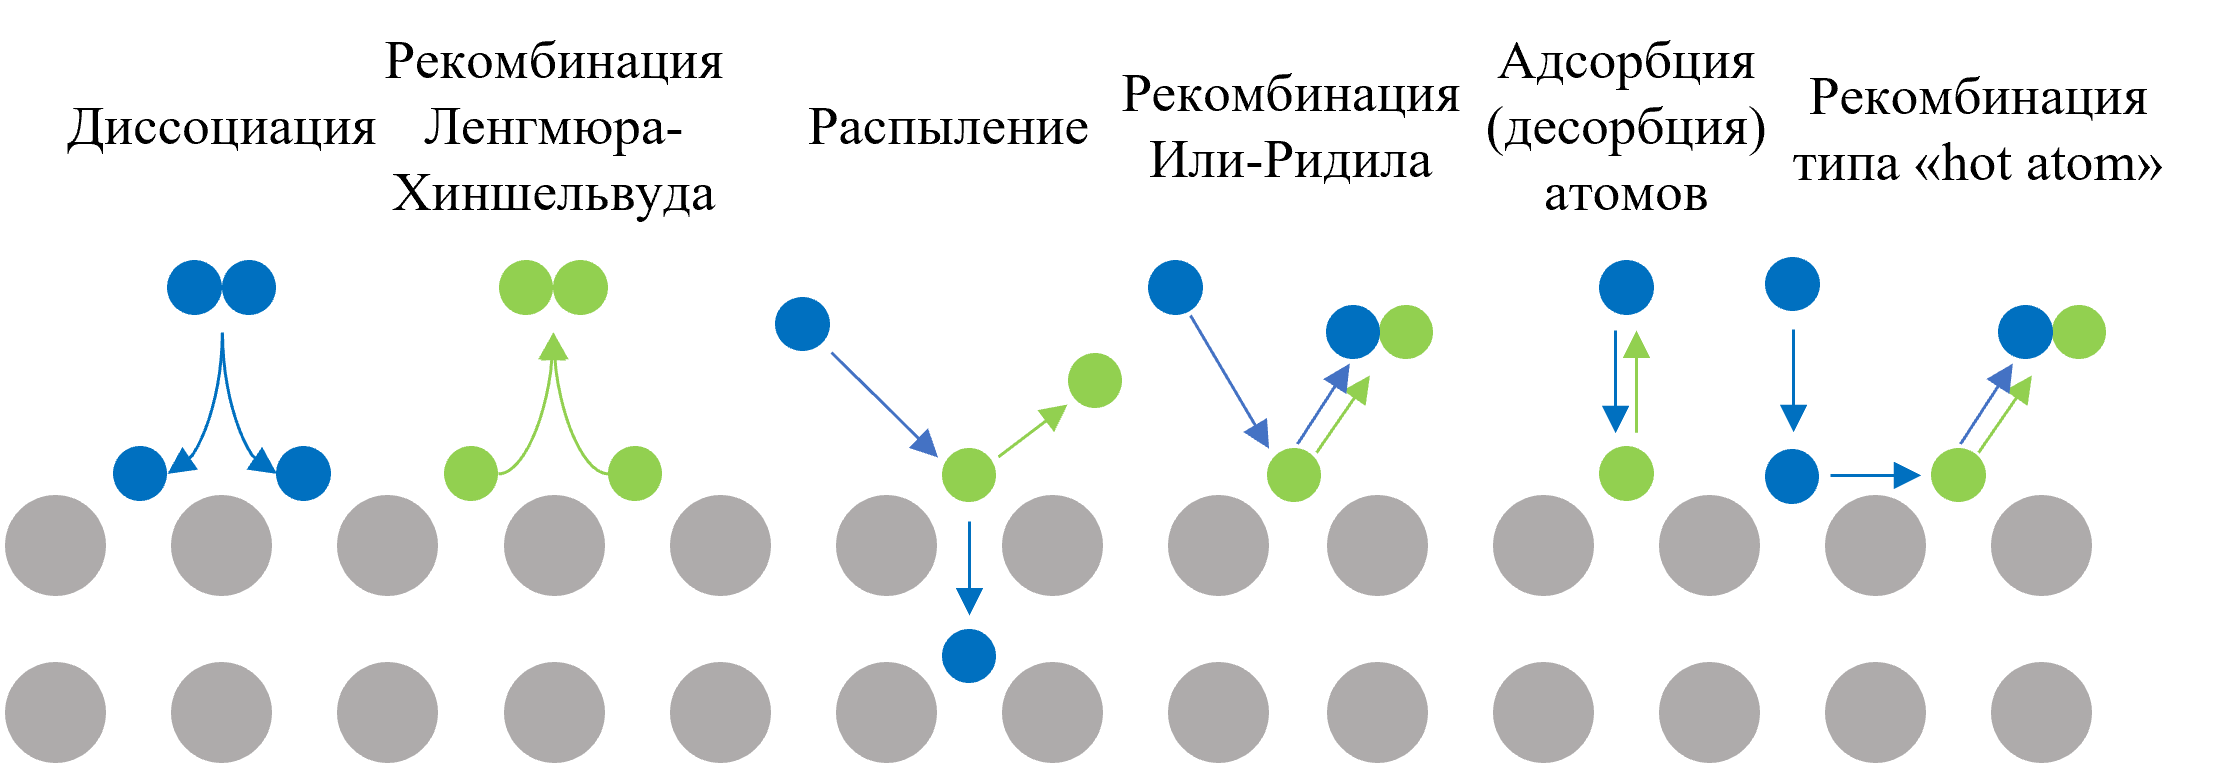
\includegraphics[scale=1]{surface_processes.png}
    }
    \caption{Схематическое представление некоторых процессы, происходящих на поверхности металла. Синие круги представляют падающие частицы (атомы или молекулы) из приповерхностной среды, зеленые круги соответствуют изначально адсорбированным атомам, серые "--- атомам материала поверхности}\label{fig:ch1/surface_processes}
\end{figure}

\begin{equation}
    K_\mathrm{S}=\cm \sqrt{P}
\end{equation}

\subsection{Закономерности накопления при стационарном плазменном облучении}

\subsubsection{Влияние потока}

\subsubsection{Влияние дозы}

\subsubsection{Влияние гелия}

\subsection{Влияние импульсных нагрузок на накопление}

\subsubsection{Импульсные тепловые нагрузки}

\subsubsection{Импульсные плазменные нагрузки}

\section{Методы дистанционного контроля содержания изотопов водорода в ОПЭ}\label{sec:ch1/sec5}

Стандартные методы контроля
Типы: ЛИД, ЛИДС, ЛИАС, ЛИИС
ЛИД
Апробация методик

\section{Выводы к Главе~\ref{ch:ch1}}\label{sec:ch1/sec6}

Для теста~\autocite{Kulagin2022a_rus}


\FloatBarrier
           % Глава 1
\chapter{Математическая модель и программный пакет для анализа динамики транспорта дейтерия в вольфраме}\label{ch:ch2}

Данная глава посвящена описанию основных математических уравнений, обобщающих раздел~\cref{subsec:ch1/sec4} и формирующих модель транспорта изотопов водорода в материалах. Кратко представлена схема численного решения использованных уравнений методом конечных элементов, реализованная в программном пакете FESTIM. Приведены детали имплементации кинетической модели, явно учитывающей поверхностные процессы, которая не была ранее реализована в коде. Также описаны результаты верификации и валидации, демонстрирующие корректность реализации и надежность имплементированной модели.

\section{Математическая модель}\label{sec:ch2/sec1}

\subsection{Транспорт изотопов водорода}

В разделе~\cref{sec:ch1/sec4} было продемонстрировано, что удержание изотопов водорода в материалах является сложным процессом, определяемым множеством элементарных процессов, как диффузия, взаимодействие с дефектами и т.д. Учет всех возможных процессов представляет из себя комплексную задачу, полноценная реализация которой маловероятна в настоящее время. В силу этого применяют методы и модели, позволяющие упростить рассмотрение, учитывая при этом наиболее важные механизмы взаимодействия.

Наиболее распространенный подход к анализу пространственно-временной эволюции концентрации изотопов водорода в материалах основан на модели Макнабба и Фостера~\cite{McNabb1963}. \fixme{В данном разделе представление теоретических аспектов для упрощения нотации будет ограничено случаем одного изотопа водорода.} Обобщение модели на случай нескольких изотопов проводится путем дублирования основных выражений для каждого типа атомов с незначительными изменениями в дефиниции процессов захвата и выхода из дефектов~\cite{Schmid2014}. В основе модели лежит разделение растворенного водорода на две фракции: подвижные атомы с концентрацией \( \cm(\mathbf{x},t) \), свободно диффундирующие по межузельным положениям, и неподвижные с концентрацией \( \ct(\mathbf{x},t) \), захваченные в дефекты разного сорта. Данный подход справедлив в приближении малой концентрации растворенного водорода и дефектов по сравнению с концентрацией атомов решетки материала, что позволяет рассматривать диффузию независимо от остальных процессов. 

В общем виде распределение концентрации подвижных атомов в момент времени \( t \) в точке \( \mathbf{x} \) геометрической области \( \Omega \), соответствующей объему материала, удовлетворяет следующей системе уравнений:
\begin{subequations}
    \label{eq:ch2/mobile_conc}
    \begin{align}
        \frac{\partial \cm}{\partial t} & = -\nabla \cdot \mathbf{J} - \sum \limits_i \frac{\partial \cti}{\partial t} + \sum \limits_j S_j, \label{eq:ch2/mobile_conc_a} \\
        \mathbf{J}                      & = -D \left( \nabla \cm + \frac{\cm Q^*}{\kBT^2} \nabla T \right). \label{eq:ch2/mobile_conc_b}
    \end{align}
\end{subequations}
Первое слагаемое в правой части уравнения~\eqref{eq:ch2/mobile_conc_a} определяет массоперенос за счет совместного влияния градиентов концентрации (закон Фика) и температуры (эффект Соре). Второй член является реакционным слагаемым, характеризующим обменный процесс между фракциями подвижных атомов и захваченных в дефекты \(i\)-типа. Последнее слагаемое учитывает совокупность объемных источников/стоков подвижных атомов со скоростью генерации/поглощения (\( S_j(\mathbf{x},t) \) в \si{\per\meter\cubed\per\second}) за счет таких процессов, как имплантация, распад/генерация трития и т.д. В уравнении массопереноса возможно также учесть адвекцию, которая играет ключевую роль при моделировании распространения водорода в движущейся жидкости~\cite{Dark2021} или в процессе формирования пленок соосаждения~\cite{Krat2020_2}. Однако в настоящей работе данный эффект не рассматривается. Параметры термоактивируемых процессов определяются из пространственно-временной эволюции поля температуры \( T(\mathbf{x},t) \).

\fixme{Для проведения основной части расчетов в данной диссертации был использован коэффициент диффузии протия в вольфраме, определенный Фернандезом и др. на основе моделирования методом DFT~\cite{Fernandez2015}. Для применения в случае транспорта дейтерия коэффициент диффузии был масштабирован на основе отношения масс изотопов (\(m_\mathrm{D}/m_\mathrm{H}\approx2\)). Итоговое выражение для коэффициента диффузии (в \si{\meter\squared\per\second}) выглядит следующим образом:
    \begin{equation}
        \label{eq:ch2/fernandez_diffusivity}
        D(T) = \frac{\num{1.93e-7}}{\sqrt{2}} \exp \left( -\frac{0.2 \, [\text{эВ}]}{\kBT} \right).
    \end{equation}
Теплота переноса дейтерия в вольфраме задавалась на основе выражения~\cref{eq:ch1/heat_transport}.} В ряде расчетов также учитывался процесс имплантации при облучении поверхности потоком частиц с плотностью \( \Gamma \) (в \si{\per\meter\squared\per\second}), который в общем виде описывается следующим выражением:
\begin{equation}
    \label{eq:ch2/impl_source}
    S(\mathbf{x},t)=\Gamma(t)\varphi(\mathbf{x}),
\end{equation}
где \( \varphi(\mathbf{x}) \) "--- пространственное распределение внедренных частиц, \si{\per\meter}.
\nomenclature[P, 31]{\( S \)}{Объемный источник/сток подвижных атомов, \si{\per\meter\cubed\per\second}}
\nomenclature[P, 32]{\(\Gamma\)}{Плотность потока атомов во время облучения, \si{\per\meter\squared\per\second}}
\nomenclature[P, 33]{\(\varphi\)}{Пространственное распределение внедренных частиц, \si{\per\meter}}

Реакционное слагаемое в выражении~\eqref{eq:ch2/mobile_conc_a} определяется процессами захвата и выхода из ловушек. Рассматриваются насыщаемые неподвижные центры захвата, вмещающие один атом водорода. Предполагается, что дефекты изолированы, то есть они не образуют протяженную сеть, а транспорт водорода между ними осуществляется посредством диффузии. Влиянием подвижности дефектов, временной эволюции их концентрации~\cite{Dark2024} и наличия ненасыщаемых дефектов ~\cite{Zibrov2024} на транспорт водорода пренебрегается.

Каждому типу дефектов ставится в соответствие концентрация захваченных в него атомов водорода (\( \cti(\mathbf{x},t) \)), концентрация дефектов (\( n_{\mathrm{t},i}(\mathbf{x}) \) в \si{\per\meter\cubed}), константы скорости захвата (\( \nu_{\mathrm{t},i}(T) \)) и освобождения (\( \nu_{\mathrm{dt},i}(T) \)). Временная эволюция концентрации атомов водорода, захваченных в тип дефекта \( i \), определяется из:
\begin{equation}
    \frac{\partial \cti}{\partial t} = \nu_{\mathrm{t},i} \cm (n_{\mathrm{t},i} - \cti) - \nu_{\mathrm{dt},i} \cti, \label{eq:ch2/trapped_conc}
\end{equation}
Первое слагаемое в правой части уравнения определяет объемный сток подвижных атомов за счет захвата в дефекты типа \( i \), величина которого зависит от локальной концентрации подвижных атомов и количества незанятых дефектов. Источником подвижных атомов является второе слагаемое, характеризующее скорость выхода атомов из дефекта типа \( i \). Важно заметить, что во втором слагаемом отсутствуют факторы, учитывающие число свободных межузельных положений или наличие соседних дефектов, что обосновывается рассмотрением малой концентрации изолированных дефектов по сравнению с плотностью атомов в решетке материала. Помимо этого, дифференциальное уравнение не учитывает переходы между энергетическими уровнями в одном дефекте, так называемый многочастичный захват. Как показывают результаты численного моделирования~\cite{Schmid2017}, в случае рассмотрения проблемы для одного изотопа водорода совокупность энергетических уровней в центре захвата может быть заменена равным количеством абстрактных дефектов с разными барьерами выхода из них. 

\fixme{Описанное представление процесса взаимодействия с дефектами позволяет качественно учитывать влияние гелия на накопление изотопов водорода. Захват большого количества атомов гелия ведет к образованию их кластеров и нанопузырей, занимающих дефекты кристаллической решетки вольфрама. Эти эффекты в свою очередь можно рассматривать как отдельные типы центров захвата для изотопов водорода, взаимодействие с которым описывается аналогичным образом, что и выше~\cite{Zibrov2024}.}

Константы скорости процессов задаются на основе закона Аррениуса с соответствующими энергиями активации захвата в дефект (\( E_{\mathrm{t},i} \)) и освобождения из него (\( E_{\mathrm{dt},i} \)):
\begin{subequations}
    \label{eq:ch2/trapping_detrapping_rates}
    \begin{align}
        \nu_{\mathrm{t},i}(T)  & = \nu_{\mathrm{t},0}^i \exp \left( -\frac{E_{\mathrm{t},i}}{\kB T} \right),    \\
        \nu_{\mathrm{dt},i}(T) & = \nu_{\mathrm{dt},0}^i \exp  \left( -\frac{E_{\mathrm{dt},i}}{\kB T} \right).
    \end{align}
\end{subequations}
Классическим подходом, позволяющим минимизировать число свободных параметров в модели, является определение константы скорости захвата на основе коэффициента диффузии и параметров кристаллической решетки материала:
\begin{equation}
    \nu_\mathrm{t}(T) \approx \frac{D(T)}{\lambda_\mathrm{IS}^2n_\mathrm{IS}},
\end{equation}
где \( n_\mathrm{IS} \) "--- объемная концентрация межузельных положений, \si{\per\meter\cubed}; \( \lambda_\mathrm{IS} \) "---  характерное расстояние между межузельными положениями, \si{\meter}. Для объемно-центрированной кубической решетки вольфрама наиболее энергетически выгодными межузельными положениями являются тетраэдрические положения, число которых вблизи атома решетки равно 6, соответственно концентрация межузельных положений \( n_\mathrm{IS} \approx \SI{3.79e29}{\per\meter\cubed} \) при концентрации вольфрама \( n_\mathrm{W}\approx\SI{6.31e28}{\per\meter\cubed} \). Характерное расстояние между такими положениями \( \lambda_\mathrm{IS}=\SI{1.1e-10}{\meter} \). Предэкспоненциальный множитель константы скорости выхода из дефектов обычно полагается равным характерной частоте тепловых колебаний атомов водорода: \( \nu_{\mathrm{dt},0} \approx \nu_0 \approx \SI{e13}{\per\second} \)~\cite{Heinola2010, Fernandez2015}.

\nomenclature[P, 34]{\( n_\mathrm{t} \)}{Концентрация дефектов, \si{\per\meter\cubed}}
\nomenclature[P, 35]{\( n_\mathrm{IS} \)}{Концентрация межузельных положений атома водорода в решетке материала, \si{\per\meter\cubed}}
\nomenclature[P, 36]{\( \nu_0 \)}{Частота тепловых колебаний атома водорода в межузельном положении или дефекте, \si{\per\second}}
\nomenclature[P, 37]{\( \lambda_\mathrm{IS} \)}{Расстояние между двумя межузельными положениями, \si{\meter}}
\nomenclature[P, 38]{\( \Omega \)}{Геометрическая область пространства}
\nomenclature[P, 39]{\( \partial\Omega \)}{Граница геометрической области}
\nomenclature[P, 40]{\( t \)}{Время, \si{\second}}

Наиболее детальное описание процессов, происходящих на открытых поверхностях исследуемого объема (границе геометрической области \( \partial\Omega \)), дается в рамках модели, явно учитывающей эволюцию концентрации адсорбированного водорода~\cite{Pisarev1997,Pick1985,Guterl2019,Hodille2017}. Пространственно-временное распределение концентрации на поверхности может быть получено на основе аналогичной реакционно-диффузионной модели, определенной в геометрической области коразмерности 1\footnote{В зависимости от размерности геометрической области, в которой рассматривается задача транспорта водорода, размерность соответствующей области для задачи об эволюции концентрации атомов на поверхности будет на единицу меньше.}. Однако в условиях взаимодействия плазмы с материалами нет необходимости учитывать все процессы. В частности, экспериментальные и теоретические работы показывают, что диффузия водорода по поверхности различных материалов энергетически более выгодна и происходит быстрее, чем другие механизмы в объеме и на поверхности~\cite{Gomer1957,Heinola2010_2,Stihl2021}. В связи с этим предполагается, что диффузия будет приводить к распределению концентрации адсорбированных атомов значительно быстрее, чем характерное время изменения других величин. Также делается допущение о неявном влиянии центров захвата на поверхности, учет которых осуществляется за счет энергетических барьеров, определяющих вероятности процессов. Исходя из этого, основное уравнение, описывающее изменение поверхностной концентрации, сводится к:
\begin{equation}
    \dfrac{d \csurf}{d t} = J_{\mathrm{bs}} - J_{\mathrm{sb}} + \Jvs, \label{eq:ch2/adsorbed_conc}
\end{equation}
где \( J_{\mathrm{bs}} \) "--- плотность потока атомов из приповерхностной области на поверхность, \si{\per\meter\squared\per\second}; \( J_{\mathrm{sb}} \)  "--- плотность потока атомов с поверхности в приповерхностную область, \si{\per\meter\squared\per\second}; \( J_{\mathrm{vs}}=J_{\mathrm{vs}}(T, \csurf, \cm) \) "--- плотность результирующего потока атомов из вакуума на поверхность, \si{\per\meter\squared\per\second}. Последнее слагаемое включает в себя все рассматриваемые механизмы адсорбции и десорбции, в которых участвуют адсорбированные атомы: \( \Jvs = \sum \limits_i J_{\mathrm{ads},i}^s - \sum \limits_i J_{\mathrm{des},i}^s \). В зависимости от порядка процесса, соответствующие потоки можно представить в общем виде: \( J_i = C_i \nu_i \csurf^j \cm^k \), где индексы \( j \) и \( k \) определяют число адсорбированных и/или растворенных атомов, участвующих в десорбции. В случае механизмов адсорбции, коэффициенты \( C_i \) будут иметь вид \( \left( 1 - c/c_{\max} \right) \) для учета возможности насыщения соответствующей области.

Уравнение связи между поверхностными и объемными процессами представляет собой граничное условие Робина для задачи транспорта водорода:
\begin{equation}
    \label{eq:ch2/surfaceBC}
    \mathbf{J} \cdot \mathbf{n} = \lambda_{\mathrm{IS}}\dfrac{\partial \cm}{\partial t} + J_{\mathrm{bs}} - J_{\mathrm{sb}} - \Jvb,
\end{equation}
где \( \mathbf{n} \) "--- внешняя нормаль к поверхности (границе \( \partial\Omega \)), \( J_{\mathrm{vs}}=J_{\mathrm{vs}}(T, \csurf, \cm) \) "--- плотность результирующего потока атомов из вакуума в приповерхностную область, \si{\per\meter\square\per\second}. Дефиниция этой величины аналогична предыдущему случаю: \( J_\mathrm{vb} = \sum \limits_i J_{\mathrm{ads},i}^b - \sum \limits_i J_{\mathrm{des},i}^b \). Качественным отличием является то, что величина \( \Jvs \) приводит к изменению концентрации атомов на поверхности, когда \( \Jvb \) влияет на концентрацию в приповерхностной области.

Плотности потоков атомов мигрирующих на поверхность и обратно определяются следующим образом~\cite{Hodille2017}:
\begin{subequations}
    \label{eq:ch2/bs_sb_fluxes}
    \begin{align}
        J_\mathrm{bs} & = \nu_{\mathrm{bs}} c_\mathrm{m} \, \left(1-\dfrac{\csurf}{n_\mathrm{s}}\right), \\
        J_\mathrm{sb} & = \nu_{\mathrm{sb}} \csurf \, \left(1-\dfrac{\cm}{n_\mathrm{IS}}\right),
    \end{align}
\end{subequations}
где \( n_\mathrm{s} \) "--- концентрация адсорбционных положений, \si{\per\meter\squared}. Эту величину можно оценить на основе концентрации атомов вольфрама: \(n_\mathrm{s}\approx (n_\mathrm{W})^{2/3}\approx \SI{1.59e19}{\per\meter\squared}\), однако более точные значения для отдельной ориентации поверхности можно получить на основе DFT расчетов~\cite{Hodille2021}. Константы скорости процессов определяются на основе закона Аррениуса:
\begin{subequations}
    \label{eq:ch2/bs_sb_nus}
    \begin{align}
        \nubs(T) = \nu_{\mathrm{bs},0} \exp \left( -\frac{E_\mathrm{bs}}{\kB T} \right), \label{eq:ch2/nu_bs} \\
        \nusb(T) = \nu_{\mathrm{sb},0} \exp \left( -\frac{E_\mathrm{sb}}{\kB T} \right). \label{eq:ch2/nu_sb}
    \end{align}
\end{subequations}
Стандартным приближением является определение константы скорости выхода на поверхность через коэффициент диффузии. В случае чистой поверхности (\( E_\mathrm{bs}\approx E_\mathrm{D}) \) можно получить достаточно компактное выражение: 
\begin{equation}
    \nu_\mathrm{bs} \approx D \lambda_\mathrm{abs} / \lambda_\mathrm{IS}^2,        
\end{equation}
где \( \lambda_\mathrm{abs} = n_\mathrm{s} / n_\mathrm{IS} \) "--- характерное расстояние между адсорбционным и межузельным положениями, \si{\meter}. Предэкспоненциальный множитель в уравнении~\cref{eq:ch2/nu_sb} полагается равным частоте колебаний атомов водорода \( \nu_0 \). В выражениях~\cref{eq:ch2/bs_sb_fluxes} члены, заключенные в скобки, учитывают возможное достижение предельной концентрации атомов водорода на поверхности и в приповерхностной области. Эти эффекты удобно описывать степенью покрытия поверхности (\( \theta \)) и степенью заполнения приповерхностной области (\( \omega \)):
\begin{subequations}
    \label{eq:ch2/theta_omega}
    \begin{align}
        \theta & = \frac{\csurf}{n_\mathrm{s}}, \\
        \omega & = \frac{\cm}{n_\mathrm{IS}}.
    \end{align}
\end{subequations}

\nomenclature[P, 41]{\( J_{\mathrm{bs}} \)}{Плотность потока атом из приповерхностной области на поверхность, \si{\per\meter\squared\per\second}}
\nomenclature[P, 42]{\( J_{\mathrm{sb}} \)}{Плотность потока атомов с поверхности в приповерхностную область, \si{\per\meter\squared\per\second}}
\nomenclature[P, 43]{\( J_{\mathrm{vs}} \)}{Плотность результирующего потока атомов из вакуума на поверхность, \si{\per\meter\squared\per\second}}
\nomenclature[P, 44]{\( J_{\mathrm{vb}} \)}{Плотность результирующего потока атомов из вакуума в приповерхностную область, \si{\per\meter\squared\per\second}}
\nomenclature[P, 45]{\( \lambda_\mathrm{abs} \)}{Характерное расстояние между адсорбционным и межузельным положениями в кристаллической решетке материала, \si{\meter}}
\nomenclature[P, 46]{\( n_\mathrm{s} \)}{Поверхностная концентрация адсорбционных положений, \si{\per\meter\squared}}
\nomenclature[P, 47]{\( \theta \)}{Степень покрытия повехности}
\nomenclature[P, 48]{\( \omega \)}{Степень заполнения приповерхностной области}

Математическое описание всех возможных процессов адсорбции и десорбции представляется нецелесообразным в настоящем разделе, так как выбор доминирующих механизмов, регулирующих эволюцию концентрации атомов, зависит от условий проведения конкретного эксперимента. Детальная информация об учитываемых механизмах в рамках каждого модельного случая приводится в соответствующих частях работы. \fixme{Однако важно отметить эффект, непосредственно определяющий вероятность десорбции адсорбированных частиц. Результаты расчетов методом DFT указывают на зависимость энергетического барьера десорбции от концентрации адсорбированных атомов (степени покрытия поверхности)~\cite{Piazza2018,Ajmalghan2019,Ferro2023}. Анализ полученных данных для случая рекомбинации молекул водорода на простейших (с низким кристаллографическими индексами Миллера) поверхностях вольфрама позволил получить выражение для аппроксимации данной зависимости в виде~\cite{Hodille2021}:
    \begin{equation}
        \label{eq:ch2/Edes_coverage}
        E_\mathrm{des}(\theta_\mathrm{D}) = E_0 + \dfrac{\Delta E}{1+\exp\left( \dfrac{\theta-\theta_0}{\delta\theta} \right)},
    \end{equation}
    где параметры $E_0$, $\Delta E$, $\theta_0$ и $\delta\theta$ являются подгоночными. Напомним, что барьер десорбции можно выразить через энергию активации и теплоту хемосорбции: \( E_\mathrm{des} = 2(E_\mathrm{c}-Q_\mathrm{c}) \). Если на поверхности отсутствует барьер хемосорбции (обычно полагается для <<чистой>> поверхности), то приведенное выражение также описывает соответствующую зависимость теплоты хемосорбции, что позволяет задавать вероятности других процессов, как прямая десорбция атомов.}

\fixme{Использование детальной модели, явно учитывающей кинетику процессов, требует задания большого числа параметров, определяющих вероятности процессов, точное значение которых известно либо для идеализированных случаев, либо неизвестно вовсе.} Часто используемым приближением является случай локального равновесия процессов вблизи поверхности (см. раздел~\cref{subsec:ch1/sec4/subsec3}). В рамках данного приближения оправдано применение коэффициента рекомбинации \( K_\mathrm{r} \) на поверхности, определяющего плотность потока десорбирующихся частиц с поверхности (граничное условие Неймана). Когда скорость рекомбинации на поверхности происходит значительно быстрее процессов в объеме, возможна редукция к граничному условию Дирихле с нулевым значением концентрации подвижных атомов на границе. Помимо этого, в части задач применялось однородное граничное условие Неймана. В совокупности были использованы три дополнительных типа граничных условий, применение которых определялось условиями рассматриваемой проблемы:
\begin{subequations}
    \begin{align}
        \mathbf{J} \cdot \mathbf{n} & = K_\mathrm{r} \cm^2 \label{eq:ch2/recombination_BC}, \\
        \mathbf{J} \cdot \mathbf{n} & = 0 \label{eq:ch2/zero_flux_BC},                      \\
        \cm                         & = 0 \label{eq:ch2/zero_conc_BC}.
    \end{align}
\end{subequations}
Уравнения~\cref{eq:ch2/mobile_conc,eq:ch2/trapped_conc,eq:ch2/adsorbed_conc} дополнялись соответствующими начальными условиями.

\subsection{Перенос тепла}

Учет температурного распределения имеет принципиальное значение, поскольку скорость протекания многих физические процессов увеличивается с температурой. Конструкционные элементы первой стенки, взаимодействующие с плазмой, испытывают воздействие интенсивных тепловых потоков и требуют активного охлаждения, что создает существенные температурные градиенты в материалах. Поэтому неотъемлемой частью моделирования транспорта водорода является определение пространственно-временной эволюции поля температур \( T(\mathbf{x},t) \). Уравнение, описывающее перенос тепла в геометрической области \( \Omega \), определяется следующим образом:
\begin{align}
    \label{eq:ch2/heat_equation}
    \rho C_p \frac{\partial T}{ \partial t} & = -\nabla \cdot \mathbf{J}_q + \sum \limits_i Q_i, \\
    \mathbf{J}_q                            & = -\kappa \nabla T,
\end{align}
где \( \rho \) "--- плотность материала, \si{\kilo\gram\per\meter\cubed}; \( C_p=C_p(T) \) "--- удельная теплоемкость материала, \si{\joule\per\kilo\gram\per\kelvin}; \( \kappa=\kappa(T) \) "--- теплопроводность материала, \si{\watt\per\meter\per\kelvin}; \( Q_i \) "--- объемный источник мощности, \si{\watt\per\meter\cubed}. Теплофизические свойства в общем случае полагаются зависящими от температуры. Все температурные зависимости физических свойств материалов, использованные в настоящей работе, приведены в Приложении~\cref{app:A}. В уравнении~\cref{eq:ch2/heat_equation} перенос тепла определяется исключительно законом Фурье, так как эффекты, связанные с переносом тепла за счет диффузионной теплопроводности, вносят гораздо меньший вклад~\cite{Martinez2021}.

В работе используются неоднородные граничные условия типа Дирихле и Неймана для определения температуры и плотности потока тепла на границе области \( \partial \Omega \):
\begin{subequations}
    \begin{align}
        \mathbf{J}_q \cdot \mathbf{n} & = q(\mathbf{x}, t) \label{eq:ch2/heat_bc_Neumann},  \\
        T                             & = f(\mathbf{x},t) \label{eq:ch2/heat_bc_Dirichlet},
    \end{align}
\end{subequations}
где \(q\) и \(f\) произвольные функции пространственных координат и времени. В каждой задаче также задавалось начальное распределение температуры.

\nomenclature[P, 49]{\( \rho \)}{Плотность, \si{\kilo\gram\per\meter\cubed}}
\nomenclature[P, 50]{\( C_p \)}{Удельная теплоемкость, \si{\joule\per\kilo\gram\per\kelvin}}
\nomenclature[P, 51]{\( \kappa \)}{Теплопроводность, \si{\watt\per\meter\per\kelvin}}
\nomenclature[P, 52]{\( Q \)}{Объемный источник/сток мощности, \si{\watt\per\meter\cubed}}
\nomenclature[P, 53]{\( q \)}{Плотность мощности на границе, \si{\watt\per\meter\squared}}

\section{Программный пакет FESTIM}\label{sec:ch2/sec2}

Рассматриваемая система дифференциальных уравнений в частных производных является нелинейной. Получение аналитического решения возможно только в отдельных случаях, зачастую требующих упрощения математической проблемы. Проведение подробного анализа возможно на основе численного моделирования. Существует ряд программных пакетов, разработанных непосредственно для решения задачи транспорта водорода, дополненной уравнением теплопроводности. В таблице~\cref{tab:codes} приведена краткая характеристика наиболее известных программных пакетов, разработанных для анализа транспорта изотопов водорода в материалах.
\begin{table}[ht]
    \centering
    \begin{threeparttable}
        \caption{Сравнение программных пакетов для моделирования транспорта изотопов водорода в материалах}
        \label{tab:codes}
        \small
        \renewcommand{\arraystretch}{1.2}%% Увеличение расстояния между рядами, для улучшения восприятия.
        \begin{tabularx}{\linewidth}{@{}>{\raggedright}X>{\centering\arraybackslash}X>{\centering\arraybackslash}X>{\centering\arraybackslash}X>{\centering\arraybackslash}X>{\centering\arraybackslash}X>{\centering\arraybackslash}X}
            \toprule
                                           & Перенос тепла & Процессы на поверхности & Размерность геометрии & Несколько изотопов & Язык программирования & Открытое ПО  \\
            \hline
            \hline
            TMAP7                          & $\checkmark$  & $\checkmark$            & 1D                    & $\checkmark$       & Fortran               &              \\
            \cite{GlenRLonghurst2008}      &               &                         &                       &                    &                       &              \\
            MHIMS                          &               & $\checkmark$            & 1D                    & $\checkmark$       & Fortran               &              \\
            \cite{Hodille2024}             &               &                         &                       &                    &                       &              \\
            CRDS                           & $\checkmark$  & $\checkmark$            & 1D                    & $\checkmark$       & Mathematica           &              \\
            \cite{Matveev2018}             &               &                         &                       &                    &                       &              \\
            TESSIM-X                       &               & $\checkmark$            & 1D                    & $\checkmark$       & Mathematica           &              \\
            \cite{Schmid2023_2}            &               &                         &                       &                    &                       &              \\
            FACE                           & $\checkmark$  & $\checkmark$            & 1D                    & $\checkmark$       & Python/Fortran        &              \\
            \cite{Smirnov2017,Smirnov2024} &               &                         &                       &                    &                       &              \\
            mHIT                           & $\checkmark$  &                         & 1D "--- 3D            &                    & COMSOL                &              \\
            \cite{Candido2021}             &               &                         &                       &                    &                       &              \\
            TMAP8                          & $\checkmark$  &                         & 1D "--- 3D            & $\checkmark$       & Python/C++            & $\checkmark$ \\
            \cite{Simon2025}               &               &                         &                       &                    &                       &              \\
            FESTIM                         & $\checkmark$  & $\checkmark$            & 1D "--- 3D            &                    & Python                & $\checkmark$ \\
            \cite{Kulagin2024}             &               &                         &                       &                    &                       &              \\
            \bottomrule
        \end{tabularx}

    \end{threeparttable}
\end{table}
\fixme{В зависимости от изначальной цели разработки, данные коды поддерживают разную степень детализации модели транспорта, размерность пространства, в котором ставится задача, и используют разные методы численного решения. Наиболее распространенным программным пакетом является TMAP7, надежность которого была продемонстрирована в десятках исследовательских работ. Существенное ограничение TMAP7 заключается в максимальном числе дефектов, которое можно учесть в расчетах. Как и большинство других кодов, приведенных в таблице~\cref{tab:codes}, TMAP7 допускает рассмотрение исключительно одномерных задач. Применительно к настоящей работе, в TMAP7 также не реализован подходящий функционал для проведения моделирования накопления изотопов водорода при длительном воздействии импульсно-периодических нагрузок.} 

\fixme{Важной особенностью также является доступность вычислительного инструмента. Большинство приведенных программных пакетов применяется внутри отдельных исследовательских групп и свободно не распространяются. Программный пакет FESTIM (Finite element simulation of tritium in materials) является одним из немногих свободно распространяемых кодов (лицензия Apache-2.0), позволяющих моделировать транспорт изотопов водорода в одно-/дву-/трехмерной геометрии, включающей несколько материалов, и с возможностью учета физических эффектов, не ограниченных списком, приведенным в предыдущем разделе~\cite{Kulagin2024}. Функционал действующей версии FESTIM не уступает новой восьмой итерации кода TMAP, которая также свободно распространяется, но, в свою очередь, позволяет учитывать все необходимые физические процессы, рассматриваемые в настоящей работе.}

Численное решение системы уравнений в частных производных в коде FESTIM основано на методе конечных элементов (МКЭ). Этот подход обеспечивает высокую точность моделирования как на микро-, так и на макроскопических пространственно-временных масштабах для объектов сложной геометрии~\cite{Nordlund2014}. Вычислительная реализация МКЭ выполняется с использованием открытой библиотеки FEniCS~\cite{FEniCS}, предоставляющей эффективные инструменты формулировки и решения дифференциальных уравнений в частных производных на языках Python и C++. FESTIM обеспечивает более высокий уровень абстракции, чем FEniCS, предоставляя окружение для специализированного решения задач транспорта изотопов водорода и теплопереноса, реализованное на языке программирования Python. Открытость исходного кода и гибкость используемых библиотек позволяет адаптировать FESTIM для решения конкретной задачи при учете физических процессов, не реализованных в действующей версии.

\nomenclature[A, 13]{МКЭ}{Метод конечных элементов}
\nomenclature[A, 14]{FESTIM}{Код для моделирования транспорта трития в материалах (Finite element simulation of tritium in materials)}

Основная идея МКЭ заключается в дискретизации рассматриваемой области \( \Omega \) на совокупность конечных элементов, в каждом из которых искомое решение уравнения в частных производных аппроксимируется гладкой функцией. Учитывая, что задачи~\cref{eq:ch2/mobile_conc,eq:ch2/heat_equation} относятся к параболическому типу, далее будет приведено краткое описание подхода к решению только задачи транспорта изотопов водорода, реализованном в коде FESTIM. Переход к дискретному представлению проблемы осуществляется с рассмотрения слабой формулировки (вариационной формы), позволяющей расширить класс функций в котором ищется приближенное решение начально-краевой задачи. Вариационная форма получается умножением обеих частей уравнения~\cref{eq:ch2/mobile_conc_a} на тестовую функцию \( v_\mathrm{m} \), обращающуюся в нуль на участке \( \partial \Omega_\mathrm{D} \subset \partial \Omega \), где определены условия типа Дирихле, и последующим интегрированием по области \( \Omega \)~\cite{FEniCS_book}:
\begin{equation}
    \label{eq:ch2/mobile_form}
    \int\limits_\Omega \frac{\partial \cm}{\partial t} v_\mathrm{m} \, dx = \int\limits_\Omega \mathbf{J} \cdot \nabla v_m \, dx - \int\limits_{\partial \Omega_\mathrm{N}} (\mathbf{J}\cdot \mathbf{n}) v_\mathrm{m} \, ds + \int\limits_\Omega S_\Sigma v_\mathrm{m} \, dx,
\end{equation}
где \( dx \) "--- элемент объема; \( ds \) "--- элемент поверхности; \( \Omega_\mathrm{N} \) "--- участок границы области, где заданы условия типа Неймана и Робина: \( \partial \Omega = \partial \Omega_\mathrm{D} \cup \partial \Omega_\mathrm{N} \), \( \partial \Omega_\mathrm{D} \cap \partial \Omega_\mathrm{N} = \varnothing \); \( S_\Sigma \) обозначает совокупность всех объемных источников. Дискретизация производной по времени проводится на основе неявного метода Эйлера:
\[
    \frac{\partial \cm}{\partial t} \approx \frac{\cm(t) - \cm(t-\Delta t)}{\Delta t},
\]
где \( \Delta t \) "--- шаг дискретизации по времени, \( \cm(t-\Delta t) \) "--- известное значение функции на предыдущем шаге. Далее будем считать, что вариационная форма справедлива в дискретном подпространстве конечных элементов, формируемом разбиением области \( \Omega \). В качестве базовых элементов для концентрации подвижных атомов водорода в коде FESTIM используются линейные непрерывные элементы Лагранжа (CG1).

При учете взаимодействия с дефектами (уравнение~\cref{eq:ch2/trapped_conc}) создается отдельная тестовая функция \( v_{\mathrm{t},i} \) для концентрации водорода, захваченного в дефект каждого типа. Соответствующая вариационная форма определяется аналогично предыдущему случаю:
\begin{equation}
    \label{eq:ch2/trapped_form}
    \int\limits_\Omega \frac{\partial \cti}{\partial t} v_\mathrm{t} \, dx = \int\limits_\Omega \left( \nu_{\mathrm{t},i} \cm (n_{\mathrm{t},i} - \cti) - \nu_{\mathrm{dt},i} \cti \right) v_{\mathrm{t},i} \, dx.
\end{equation}
Предусматривается возможность использования как линейных непрерывных элементов Лагранжа (CG1), так и линейных разрывных элементов Лагранжа (Галеркина, DG1). Снятие условия на непрерывность функции позволяет иногда избежать развития осцилляций численного решения вблизи границ элементов, например, при рассмотрении кусочно-гладких профилей дефектов.

Имплементация модели, учитывающая кинетику процессов на поверхности, была проведена в рамках настоящей диссертации. В текущей версии кода (1.4) моделирование процессов на поверхности возможно только в нульмерном приближении при совместном решении задачи транспорта в одномерном приближении. Однако это упрощение не ограничивает существенно применимость модели, поскольку большинство лабораторных экспериментов (ТДС, эксперименты по наводораживанию, эксперименты по проницаемости и т.д.) обычно могут быть описаны в рамках одномерного приближения. Переход к слабой формулировке возможен путем умножения уравнения~\cref{eq:ch2/adsorbed_conc} на тестовую функцию \( v_\mathrm{s} \) и интегрирования по границе области:
\begin{equation}
    \label{eq:ch2/adsorbed_form}
    \int\limits_{\partial \Omega_\mathrm{N}} \frac{\partial \csurf}{\partial t} v_\mathrm{s} \, ds = \int\limits_{\partial \Omega_\mathrm{N}} \left( \Jbs - \Jsb + \Jvs \right) v_\mathrm{s} \, ds.
\end{equation}
Данная процедура повторяется для каждой из границ расчетной области, на которой рассматривается эволюция концентрации адсорбированных атомов. Учитывая нульмерность модели, пробная и тестовые функции определены в пространстве вещественных чисел.

Объединение выражений~\cref{eq:ch2/mobile_form,eq:ch2/trapped_form,eq:ch2/adsorbed_form} приводит в общем случае к нелинейной вариационной задаче вида:
\[
    F(\mathbf{c};\mathbf{v})=0,
\]
где \( \mathbf{c}=(\cm,c_{\mathrm{t},1},c_{\mathrm{t},2},\ldots,c_{\mathrm{t},n},c_{\mathrm{s},1},c_{\mathrm{s},2}) \); \( \mathbf{v}=(v_\mathrm{m},v_{\mathrm{t},1},v_{\mathrm{t},2},\ldots,v_{\mathrm{t},n},v_{\mathrm{s},1},v_{\mathrm{s},2}) \). Равенство выполняется для любых тестовых функций из соответствующего подпространства. Разложение искомых и тестовых функций по базису подпространства конечных элементов приводит к системе нелинейных алгебраических уравнений относительно коэффициентов разложения. Решение системы уравнений в коде FESTIM осуществляется итерационным методом Ньютона. Стоит отметить, что со стороны пользователя требуется только поставить начально-краевую задачу, когда выбор базисных функций, построение вариационной формы, решение системы нелинейных уравнений и экспорт полученных результатов осуществляются внутри программного пакета.

Проверка корректности реализации численной схемы решения рассматриваемой задачи (верификация) и анализ применимости модели для описания эмпирически наблюдаемых процессов (валидация) являются необходимыми условиями использования любого программного пакета, предназначенного для исследования физических явлений. Любые изменения в коде FESTIM проходят тщательную проверку благодаря системе непрерывной интеграции, включающей сотни автоматических тестов как отдельных модулей, так всего пакета. Набор тестов также проводит верификационные проверки отдельных физических модулей, например блок решения уравнения теплопроводности, методами точных и построенных решений. Валидация кода FESTIM проводится на основе литературных данных. Ключевые тестовые задачи представлены в свободно распространяемой книге по верификации и валидации кода FESTIM~\cite{FESTIM_VV}.

\section{Верификация и валидация модели, учитывающей процессы на поверхности}\label{sec:ch2/sec3}

Раннее отмечалось, что модель~\cref{eq:ch2/adsorbed_conc}, явно учитывающая эволюцию концентрации адсорбированного водорода, была внедрена в код FESTIM в рамках настоящей работы. Как и все основные модули кода, модель требовала проведения верификации и валидации для демонстрации надежности и корректности реализации. Верификация модели проводилась с помощью метода построенных решений (Method of manufactured solutions, MMS), когда валидация осуществлялась путем воспроизведения результатов четырех экспериментальных работ по накоплению изотопов водорода в различных материалах~\cite{Kulagin2025_IJHE}. Все исходные коды, использованные для проверки корректности имплементации модели, распространяются свободно~\cite{vladimir_kulagin_2025_14738004, Kulagin_PhD_2025} и включены в онлайн-книгу с результатами верификации и валидации кода FESTIM~\cite{FESTIM_VV}. В рамках данного раздела приведены краткие результаты проведенной проверки.

\subsection{Верификация модели}\label{sec:ch2/sec3/subsec1}
Верификация модели~\cref{eq:ch2/adsorbed_conc}, учитывающей процессы на поверхности, проводилась с помощью метода построенных решений решений. MMS широко используется для оценки точности численных методов решения систем дифференциальных уравнений в частных производных~\cite{Roache2002,Oberkampf_Roy_2010}. Подход заключается в выборе аналитической функции, лежащей в области определения решения системы заданных уравнений. Затем на основе данной функции определяются параметры объемных источников, начальные и граничные условия, при которых функция становится решением системы. На основе определенных параметров и начально-краевых условий требуется получить численное решение рассматриваемой проблемы. Ошибка между <<построенным>> и численным решениями характеризует точность численного метода.

Рассмотрим упрощенную задачу диффузии в области \( \Omega: x \in [0,L] \cup t \in [0,t_f], \, L=1, \, t_\mathrm{f}=5 \):
\begin{equation}
    \label{eq:ch2/manufactured_diffusion}
    \frac{\partial \cm}{\partial t} = D \frac{\partial^2 \cm}{\partial x^2} + S,
\end{equation}
наряду с которой будем также рассматривать дифференциальное уравнение~\cref{eq:ch2/adsorbed_conc}. Взаимодействие с дефектами не влияет на процессы на поверхности, поэтому этот эффект не учитывается. В качестве <<построенного>> решения выберем следующую функцию:
\begin{equation}
    \label{eq:ch2/manufactured_solution}
    c_\mathrm{m, exact}=1+2x^2+x+2t.
\end{equation}
На левой границе области (\( x=0 \)) зададим уравнение~\cref{eq:ch2/surfaceBC}, а на правой (\( x=L \)) потребуем выполнения равенства:
\begin{equation}
    \cm(x=L, t)=c_\mathrm{m, exact}(x=L, t).
\end{equation}
В качестве параметров модели выберем: \( D=7 \), \( \nubs=3 \), \( \nusb = 2n_\mathrm{IS}/n_\mathrm{s} \), \(n_\mathrm{IS}=20 \), \(n_\mathrm{s}=5 \), \( \lambda_\mathrm{IS}=2\).

Подстановка выбранных функции и параметров в выражения~\cref{eq:ch2/manufactured_diffusion,eq:ch2/adsorbed_conc} позволяет получить выражение для объемного источника, концентрации адсорбированных атомов (\( c_{\mathrm{s,exact}} \)) и плотности потока из вакуума на поверхность:
\begin{subequations}
    \begin{align}
        S                   & = 2(1-2D),                                                                                                         \\
        c_\mathrm{s, exact} & = n_\mathrm{s} \dfrac{3(1+2t) + 2\lambda_\mathrm{IS}-D}{2n_\mathrm{IS}+1+2t},                                      \\
        J_{\mathrm{vs}}     & = 2n_\mathrm{s} \dfrac{6n_\mathrm{IS} - 2\lambda_\mathrm{IS}+D}{(2n_\mathrm{IS}+1+2t)^2} + 2\lambda_\mathrm{IS}-D.
    \end{align}
\end{subequations}
В качестве начальных условий полагаем:
\begin{subequations}
    \begin{align}
        \cm(x, t=0) & = c_\mathrm{m, exact}(x, t=0) \\
        \csurf(t=0) & = c_\mathrm{s, exact}(t=0)
    \end{align}
\end{subequations}
Моделирование проводится на равномерной сетке, состоящей из 1000 элементов, с фиксированным размером временного шага. Оценка точности численного решения (\( c_\mathrm{m, computed} \), \( c_\mathrm{s, computed} \)) проводилась на основе \( L^2 \)-нормы:
\begin{subequations}
    \begin{align}
        E_\mathrm{m} & = \sqrt{ \int\limits_\Omega \left(c_\mathrm{m, exact}-c_\mathrm{m, computed}\right)^2 d\Omega },      \\
        E_\mathrm{s} & = \sqrt{ \int\limits_0^{t_\mathrm{f}} \left(c_\mathrm{s, exact}-c_\mathrm{s, computed}\right)^2 dt }.
    \end{align}
\end{subequations}

На рисунке~\cref{fig:ch2/MMS_a,fig:ch2/MMS_b} приведено сравнение результатов. Численные решения хорошо согласуются с точными: \(E_\mathrm{m} = \num{2.28e-5} \) и \( E_\mathrm{s}= \num{4.36e-5} \).
\begin{figure}[ht]
    \centerfloat{
        \hfill
        \subcaptionbox[List-of-Figures entry]{\label{fig:ch2/MMS_a}}{%
            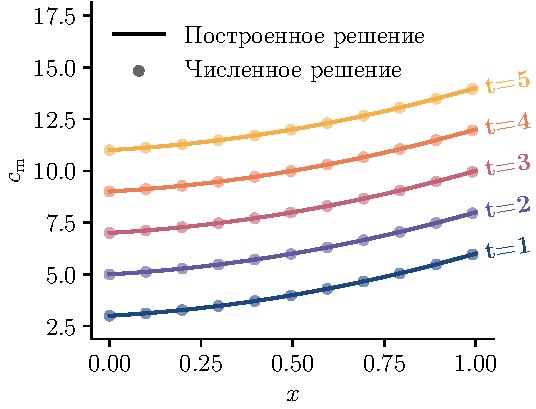
\includegraphics[scale=1]{MMS_a.pdf}}
        \hfill
        \subcaptionbox{\label{fig:ch2/MMS_b}}{%
            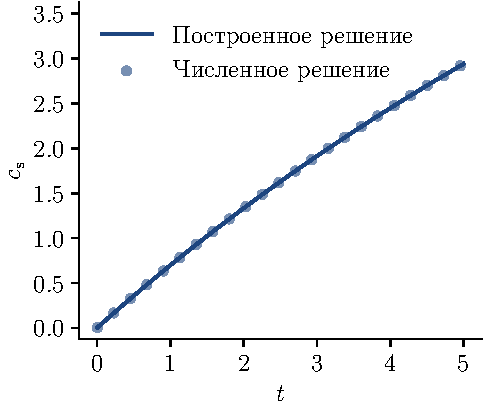
\includegraphics[scale=1]{MMS_b.pdf}} \\
        \subcaptionbox{\label{fig:ch2/MMS_c}}{%
            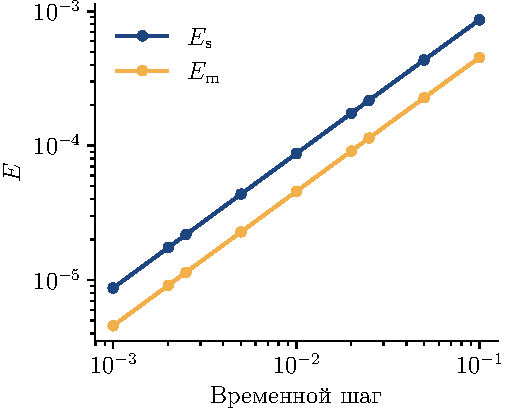
\includegraphics[scale=1]{MMS_c.pdf}}
    }
    \caption{Эволюция профиля концентрации подвижных атомов (a) и временная эволюция концентрации адсорбированных атомов (б) при временном шаге \num{5e-3}; (в) зависимость отклонения численных решений от аналитических}\label{fig:ch2/MMS}
\end{figure}
Учитывая нульмерность уравнения~\cref{eq:ch2/adsorbed_conc}, интерес представляет анализ сходимости по временной дискретизации. Из рисунка~\cref{fig:ch2/MMS_c} видно, что ошибки для обеих переменных линейно уменьшаются совместно с размером шага по времени, что ожидаемо ввиду использования схемы Эйлера для аппроксимации временных производных.

\subsection{Валидация модели}\label{sec:ch2/sec3/subsec2}

В этом разделе представлены четыре валидационных теста, использованных для проверки реализованной модели~\cref{eq:ch2/adsorbed_conc}. \fixme{Они воспроизводят эксперименты по накоплению изотопов водорода в титане, вольфраме и стали EUROFER при облучении поверхности потоками атомов или молекул с низкой энергией. Данные эксперименты были проанализированы ранее в иных работах, поэтому далее будет представлено краткое описание экспериментальных условий.} Три тестовых случая дополнительно включают сравнение с результатами моделирования, проведенного ранее с помощью кодов MHIMS~\cite{Hodille2024} или TESSIM-X~\cite{Schmid2023_2}. Во всех случаях рассматривается транспорт водорода в одномерном приближении, определяемый законом Фика, а эволюция температуры задается по известному закону. С точки зрения моделирования, основным отличием являются разные предположения о процессах, протекающих на поверхности в частном эксперименте.

\subsubsection{Эксперимент по абсорбции протия в титане}
Первый тестовый случай воспроизводит эксперименты по абсорбции протия в титане при различных значениях температуры~\cite{Hirooka1981}. Эксперименты по абсорбции проводились в вакуумной камере при базовом давлении $p_\mathrm{H_2}=\SI{1.3e4}{\pascal}$ с образцами размером $10\times13\times1$\,мм. Образцы поддерживались при постоянной температуре в диапазоне от \SI{473}{K} до \SI{923}{K}. \fixme{Содержание протия в титане оценивалось по изменению парциального давления в камере.}

\fixme{Учитывая низкую энергию тепловых молекул, естественно полагать, что основным процессом, определяющим накопление, будет адсорбция на поверхности. Также стоит заметить, что эксперименты проводились при относительно высоком давлении, что позволяет ожидать быстрого насыщения поверхности.} Соответственно, в моделировании полагается, что эволюция поверхностной концентрации протия определяется ​​адсорбцией ($J_{\mathrm{ads}}^{\mathrm{H_2}}$) и рекомбинацией ($J_\mathrm{des}^{\mathrm{H_2}}$) молекул~\cite{Shimohata2021}. Таким образом, результирующая плотность потока из вакуума на поверхность в уравнении~\cref{eq:ch2/adsorbed_conc} определяется следующими выражениями:
\begin{subequations}
    \label{eq:ch2/case1_surf_proc}
    \begin{align}
        \Jvs                          & = J_\mathrm{ads}^{\mathrm{H_2}}-J_\mathrm{des}^{\mathrm{H_2}},                                 \\
        J_\mathrm{ads}^{\mathrm{H_2}} & = 2 \, \nu_{\mathrm{ads}}^{\mathrm{H_2}} p_\mathrm{H_2} \, \left(1-\theta_\mathrm{H}\right)^2, \\
        J_\mathrm{des}^{\mathrm{H_2}} & = 2 \, \nu_\mathrm{des}^{\mathrm{H_2}} \, \csurf^2, \label{eq:ch2/molecular_desortion}
    \end{align}
\end{subequations}
где \( \theta_\mathrm{H}=\csurf/n_\mathrm{s} \) "--- степень покрытия поверхности титана протием; \( \nu_\mathrm{des}^{\mathrm{H_2}}=\nu_\mathrm{des,0}^{\mathrm{H_2}} \exp(-E_\mathrm{des}/k_\mathrm{B} T) \) "--- константа скорости десорбции за счет рекомбинации двух атомов на поверхности. Константа скорости адсорбции определяется как:
\begin{equation}
    \label{eq:ch2/nu_ads_P}
    \nu_{\mathrm{ads}}^{\mathrm{H_2}} = \dfrac{\Phi}{\sqrt{2\pi m_\mathrm{H_2}k_\mathrm{B} T}},
\end{equation}
где \( \Phi = \Phi_0 \exp \left( -E_\mathrm{diss}/\kBT \right) \) "--- коэффициент прилипания; $m_\mathrm{H_2}$ "--- масса молекулы протия, \si{\kilo\gram}. Давление в камере рассчитывается из уравнения состояния идеального газа:
\begin{equation}
    p_\mathrm{H_2} = \left( \frac{p_\mathrm{H_2,0} V_\mathrm{ch}}{k_\mathrm{B} T} + \frac{N_0-N}{2} \right) \frac{k_\mathrm{B} T}{V_\mathrm{ch}},
\end{equation}
где \( p_\mathrm{H_2,0} \) "--- начальное давление в камере, \si{\pascal}; \( V_\mathrm{ch} \) "--- объем камеры, \si{\meter\cubed}; \( N_0 \) "--- начальное число атомов протия в титане; \( N \) "--- действующее число атомов протия в титане. Содержание протия в титане определяется как сумма интегрального числа атомов на поверхности и в объеме.

\nomenclature[P, 54]{\( \nu_\mathrm{ads}^{\mathrm{I_2}} \)}{Константа скорости адсорбции молекул изотопа водорода I из газовой фазы, \si{\per\meter\squared\per\second\per\pascal}}
\nomenclature[P, 55]{\( \nu_\mathrm{des}^{\mathrm{I_2}} \)}{Константа скорости десорбции атомов изотопа водорода I по каналу Ленгмюра"--~Хиншельвуда, \si{\meter\squared\per\second}}
\nomenclature[P, 56]{\( \nu_\mathrm{des}^{\mathrm{I}} \)}{Константа скорости десорбции атомов изотопа водорода I по каналу Или"--~Ридила, \si{\per\second}}
\nomenclature[P, 57]{\( \Phi \)}{Коэффициент прилипания}
\nomenclature[P, 58]{\( m_{\mathrm{I}} \)}{Масса молекулы изотопа водорода I, \si{\kilo\gram}}
\nomenclature[P, 59]{\( V \)}{Объем, \si{\meter\cubed}}
\nomenclature[P, 60]{\( N \)}{Число атомов изотопа водорода}
\nomenclature[P, 61]{\( L \)}{Толщина геометрии, \si{\meter}}

Константы скорости переходов между поверхностью и приповерхностной областью определяются в соответствии с законом Аррениуса (уравнения \cref{eq:ch2/bs_sb_nus}). Взаимодействие с центрами захвата не учитывается. Количество межузельных и адсорбционных положений оценивается через объемную концентрацию атомов титана ($n_\mathrm{Ti}$ в \si{\per\meter\cubed}). Начальное содержание протия в титане принимается равным нулю. Моделирование проводилось только для половины геометрии на сетке, состоящей из 1000 равных элементов, с условием симметрии (нулевым потоком) на правой границе и моделью, учитывающей процессы на поверхности, определенной на левой границе.

Для воспроизведения экспериментальных зависимостей была проведена процедура автоматической оптимизации параметров~\cite{Delaporte-Mathurin2021}. Процедура заключается в построении функции ошибки, характеризующей отклонение численных результатов от экспериментальных. В качестве функции ошибки использовалось cреднеквадратическое отклонение по всей выборке. Затем проводится оптимизация параметров для минимизации ошибки между данными. В рамках работы для этой процедуры применялся алгоритм Недлера-Мида. Параметры $\nu_\mathrm{des,0}$, $E_\mathrm{des}$, $\nu_\mathrm{bs,0}$, $E_\mathrm{bs}$, $\nu_\mathrm{sb,0}$ и $E_\mathrm{sb}$ рассматривалась как свободные. Для первоначального предположения использовались соответствующие значения, представленные в работе~\cite{Shimohata2021}. Совокупность входных параметров обобщена в таблице~\cref{tab:case1_inputs}.

Степень согласия между результатами моделирования и эксперимента количественно определялась с помощью среднеквадратической ошибки:
\begin{equation}
    \mathrm{RMSE} = \sqrt{\dfrac{1}{N} \sum \limits_{i=1}^N(x_{\mathrm{sim},i}-x_{\mathrm{exp},i})^2},
\end{equation}
где $x_{\mathrm{sim},i}$ и $x_{\mathrm{exp},i}$ представляют собой рассчитанные и экспериментальные значения анализируемой величины (в данном случае содержание протия в титане).

Сравнение результатов приведено на рисунке~\cref{fig:ch2/val1}. Достигнуто разумное согласие (\( \mathrm{RMSE}=\num{2.915e-2} \)) между результатами моделирования в коде FESTIM и экспериментальными данными во всем диапазоне температур при использовании одного набора параметров.
\begin{figure}[ht]
    \centerfloat{
        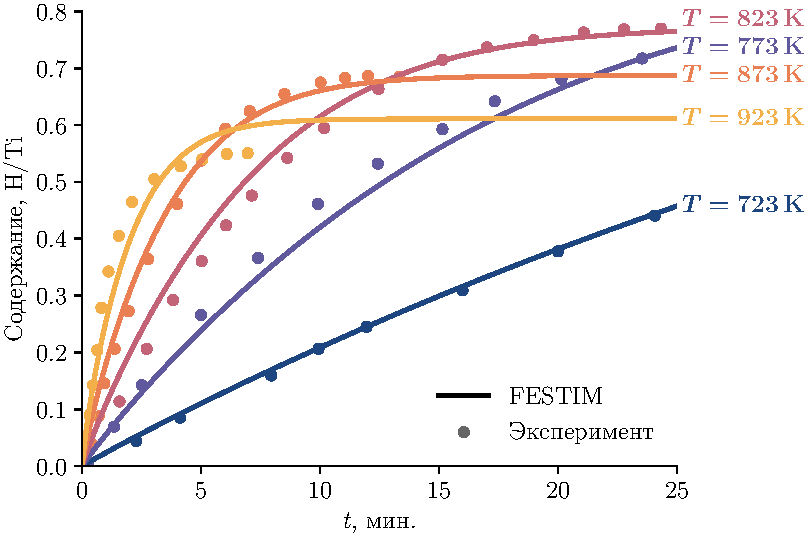
\includegraphics[scale=1]{val1.pdf}
    }
    \caption{Временные зависимости содержания протия в титане при различных температурах}\label{fig:ch2/val1}
\end{figure}

\subsubsection{Эксперимент по адсорбции дейтерия на поверхности вольфрама, покрытой атомами кислорода}
\fixme{Второй валидационный тест воспроизводит экспериментальные результаты по десорбции дейтерия с поверхности вольфрама, покрытой атомами кислорода~\cite{Dunand2022}. Вся серия экспериментов проводилась \textit{in situ} при сверхнизком базовом давлении в камера \( \approx \SI{5e-8}{\pascal} \). Три монокристаллических образца (толщиной \(L=\SI{2}{\milli\meter}\)) были подготовлены с различной степенью покрытия поверхности кислородом \( \theta_\mathrm{O}=0;~0.5;~0.75 \). Получение атомарно чистой поверхности происходило за счет цикличного повторения (\(\approx\)500 раз) двух процедур: нагрева поверхности лазерным импульсом в атмосфере кислорода с целью удаления углерода (за счет образовании CO-молекул) с последующим нагревом образца до температуры выше \SI{2000}{\kelvin} для инициирования десорбции кислорода. Достижение заданной степени покрытия поверхности кислородом осуществлялось при выдержке в атмосфере кислорода. Состояние поверхности контролировалось при помощи метода дифракции медленных электронов на всех этапах подготовки образцов. Полученные образцы затем подвергались экспозиции в атмосфере дейтерия при давлении в камере $p_\mathrm{D_2}=\SI{2e-5}{\pascal}$ и комнатной температуре (\SI{300}{K}). Экспозиция длилась \SI{3000}{\second}, за которой следовала фаза хранения в течение \SI{1}{\hour}. После этого были проведены ТДС-измерения потока десорбированных частиц с постоянной скоростью нагрева равной \SI{5}{\kelvin\per\second}. Отмечается, что в ходе экспозиции в атмосфере дейтерия происходила аморфизация изначальной поверхностной конфигурации атомов, однако степень покрытия поверхности кислородом оставалась высокой. Также в ходе ТДС не наблюдался выход молекул тяжелой воды.}

Следуя работе~\cite{Hodille2024}, предполагается, что эволюция поверхностной концентрации $\csurf$ определяется адсорбцией дейтерия из газовой фазы и десорбцией молекул с поверхности, аналогично первому тестовому случаю (уравнения~\eqref{eq:ch2/case1_surf_proc}). Константа скорости адсорбции рассчитывается согласно уравнению~\cref{eq:ch2/nu_ads_P} с использованием массы молекулы и парциального давления дейтерия в камере. Полагается, что наличие кислорода на поверхности вольфрама влияет на распределение потенциальной энергии и на количество доступных мест для адсорбции:
\begin{equation}
    n_\mathrm{s}(\theta_\mathrm{O}) = n_\mathrm{s}(0)(1-\theta_\mathrm{O}).
\end{equation}

Согласно расчетам методом DFT, энергия активации десорбции зависит от степени покрытия поверхности~\cite{Piazza2018,Ajmalghan2019,Ferro2023}. Чтобы учесть этот эффект, в работе~\cite{Hodille2024} использовалась следующая константа скорости десорбции:
\begin{subequations}
    \label{eq:ch2/nu_des_mol_s}
    \begin{align}
        \nu_\mathrm{des}^{\mathrm{D_2}}   & = \nu_\mathrm{des,0}^{\mathrm{D_2}} \exp \left( -\frac{E_\mathrm{des}(\theta)}{k_\mathrm{B} T} \right), \\
        \nu_\mathrm{des,0}^{\mathrm{D_2}} & = \nu_0\lambda_\mathrm{des}^2,
    \end{align}
\end{subequations}
где $\nu_0$ "--- характерная частота колебаний атомов дейтерия, \si{\per\second}; $\lambda_\mathrm{des}=1/\sqrt{n_\mathrm{s}}$ "--- характерное расстояние между адсорбционными положениями, \si{\meter}. Зависимость энергии активации для десорбции($E_\mathrm{des}$ в \si{\electronvolt}) была аппроксимирована следующим выражением:
\begin{subequations}
    \begin{align}
        E_\mathrm{des}(\theta_\mathrm{D}) & = E_\mathrm{1}(\theta_\mathrm{D})\left( 1-a \exp\left( -b (1-\theta_\mathrm{D}) \right) \right), \label{eq:ch2/case2_Edes} \\
        E_\mathrm{1}(\theta_\mathrm{D})   & = E_0 + \dfrac{\Delta E}{1+\exp\left( \dfrac{\theta_\mathrm{D}-\theta_\mathrm{D,0}}{\delta\theta_\mathrm{D}} \right)}.
    \end{align}
\end{subequations}
Данная совокупность выражений является модификацией уравнения~\cref{eq:ch2/Edes_coverage}. В данном случае $E_\mathrm{1}$ определяет изменение энергии десорбции ниже насыщения. Множитель в скобках в уравнении (\ref{eq:ch2/case2_Edes}) отвечает за экспоненциальное уменьшение энергии десорбции выше насыщения~\cite{Ferro2023, Matveev2018}.

\nomenclature[P, 62]{\( \lambda_\mathrm{des} \)}{Характерное расстояние между адсорбционными положениями, \si{\meter}}

Используются зависящие от температуры (уравнения~\eqref{eq:ch2/bs_sb_nus}) скорости переходов атомов дейтерия между поверхностью и приповерхностной областью. Энергия активации выхода на поверхность задается на основе диффузионного барьера: $E_\mathrm{bs}\approx E_\mathrm{D}$, с предэкспоненциальным множителем: $\nu_\mathrm{bs,0}=\nu_0 n_\mathrm{s} / n_\mathrm{IS}$. Константа скорости абсорбции полагается зависящей от концентрации дейтерия на поверхности:
\begin{subequations}
    \begin{align}
        \nusb                 & = \nu_\mathrm{sb,0}\exp\left( -\frac{E_\mathrm{sb}(\theta)}{k_\mathrm{B} T} \right),                          \\
        E_\mathrm{sb}(\theta) & = \frac{E_\mathrm{des}(\theta) - E_\mathrm{diss}}{2} + E_\mathrm{bs} + Q_\mathrm{s}, \label{eq:ch2/case2_Esb}
    \end{align}
\end{subequations}
где $\nu_\mathrm{sb,0} = \nu_0$; $Q_\mathrm{s}=\SI{1}{\electronvolt}$~\cite{Fernandez2015} "--- теплота раствора дейтерия в вольфраме.

Поскольку вероятность абсорбции при комнатной температуре пренебрежимо мала, центры захвата в текущем случае не рассматриваются, \fixme{а все основные процессы происходят на поверхности}. Однако для полной постановки задачи транспорта в коде FESTIM требуется задать параметры объемных процессов. Коэффициент диффузии дейтерия в вольфраме определяется путем масштабирования соответствующего коэффициента для протия (выражение~\cref{eq:ch2/fernandez_diffusivity}). Как и в предыдущем случае, количество межузельных и адсорбционных положений оценивается через объемную концентрацию атомов вольфрама ($n_\mathrm{W}$).

Моделирование проводилось на равномерной сетке из 500 элементов с условием~\cref{eq:ch2/adsorbed_conc} на левой границе ($x=0$) и однородным граничным условием Дирихле на правой ($\cm(x=L)=0$). В начале моделирования предполагается, что концентрация дейтерия в вольфраме равна нулю. Все входные параметры моделирования обобщены в таблицах~\cref{tab:case2_inputs,tab:case2_Edes_params}. Сравнение результатов численных расчетов приведено на рисунке~\cref{fig:ch2/val2}.

\begin{figure}[ht]
    \centerfloat{
        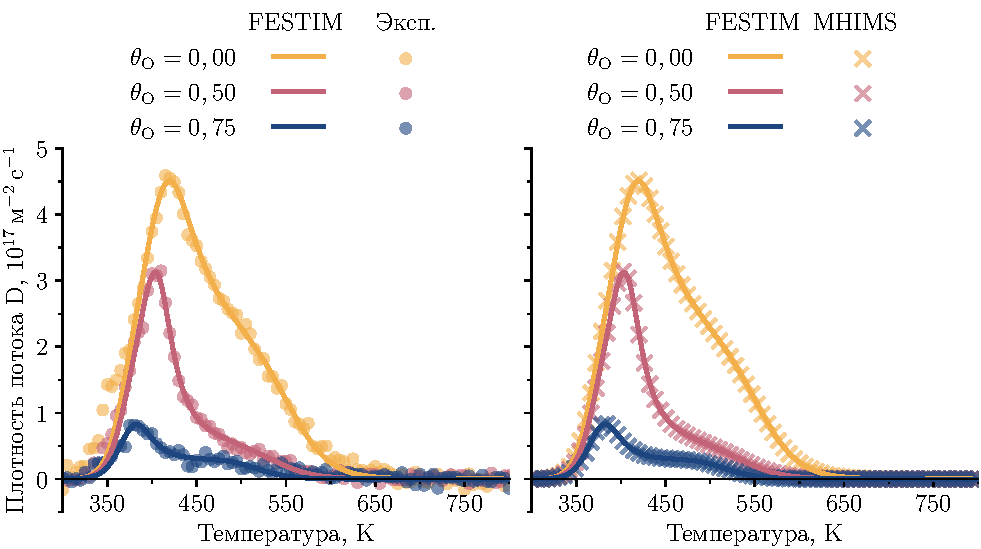
\includegraphics[scale=1]{val2.pdf}
    }
    \caption{ТДС-спектры дейтерия, десорбированного с поверхности вольфрама при различным значениях степени покрытия поверхности кислородом. Сравнение с экспериментальными данными (слева) и численными результатами, полученными в коде MHIMS (справа)}\label{fig:ch2/val2}
\end{figure}

Все зависимости демонстрируют пик в области низких температур с затяжным высокотемпературным плечом. С увеличением концентрации кислорода на поверхности пик смещается в область более низких температур, а общее количество вышедшего дейтерия спадает из-за меньшего числа доступных мест для адсорбции. Смоделированные зависимости демонстрируют хорошее согласие с экспериментальными данными и совпадают с результатами, полученными в коде MHIMS. Среднеквадратические отклонения между численными результатами и экспериментальными данными находятся на уровне шума и равны \SI{2.1e16}{\per\meter\squared\per\second} при \( \theta_\mathrm{O}=0 \); \SI{8.8e15}{\per\meter\squared\per\second} при \( \theta_\mathrm{O}=0,5 \); \SI{7.2e15}{\per\meter\squared\per\second} при \( \theta_\mathrm{O}=0,75 \). \fixme{Следует отметить, что полученное согласие не позволяет получить детальное представление о протекающих на поверхности процессах. Учитывая то, что в эксперименте было обнаружено изменение атомарной конфигурации на поверхности, можно предположить, что кинетика процессов, определяющих, десорбцию также менялась в течение облучения.}

\subsubsection{Эксперимент по облучению вольфрама низкоэнергетичными атомами дейтерия}
Третий случай проверки воспроизводит результаты МЯР-измерений распределения дейтерия в вольфраме после облучения потоком атомов с низкой энергией~\cite{Markelj2016}. Экспериментальная процедура включала три основные фазы. Поликристаллический образец вольфрама толщиной \(L=\SI{0.8}{\milli\meter}\) был предварительно облучен ионами вольфрама с энергией \SI{20}{\mega\electronvolt} до дозы \SI{7.8e17}{\per\meter\squared} для создания дефектов в приповерхностном слое. Затем образец был подвергнут облучению низкоэнергетическими (\(\approx\SI{0.3}{\electronvolt}\)) атомами дейтерия с плотностью потока \(\Gamma_\mathrm{D}=\SI{5.8e18}{\per\meter\squared\per\second}\) при температуре образца \SI{600}{\kelvin}. Облучение длилось до тех пор, пока не была достигнута доза \SI{e24}{\per\meter\squared}. На финальном этапе проводилось обезгаживание образца в течение \SI{43}{\hour} при температуре равной \SI{600}{K}. Все этапы экспериментов проводились \textit{in situ}.

Численная модель учитывает три процесса на поверхности: адсорбция низкоэнергетических атомов ($J_\mathrm{ads}^\mathrm{D}$), десорбция по механизму Ленгмюра"--~Хиншельвуда ($J_\mathrm{des}^\mathrm{D_2}$) и десорбция по механизму Эли-Ридила ($J_\mathrm{des}^{\mathrm{D}}$). Плотности потока атомов, обусловленные упомянутыми механизмами, определяются на основе выражений:
\begin{subequations}
    \label{eq:ch2/case3_Jvs}
    \begin{align}
        \Jvs                        & = J_\mathrm{ads}^\mathrm{D}-J_\mathrm{des}^\mathrm{D_2}-J_\mathrm{des}^\mathrm{D}, \\
        J_\mathrm{ads}^\mathrm{D}   & = \Gamma_\mathrm{D} \Phi \, \left( 1 - \theta_\mathrm{D} \right),                  \\
        J_\mathrm{des}^\mathrm{D_2} & = 2 \, \nu_\mathrm{des}^\mathrm{D_2} \, \csurf^2,                                  \\
        J_\mathrm{des}^\mathrm{D}   & = \nu_\mathrm{des}^\mathrm{D} \, \csurf,
    \end{align}
\end{subequations}
где \( \nu_\mathrm{des}^\mathrm{D} = \Gamma_\mathrm{D} \sigma_\mathrm{ER} \) "--- константа скорости десорбции за счет рекомбинации адсорбированного и приходящего атомов дейтерия, \si{\per\second}; \( \sigma_\mathrm{ER} \) "--- поперечное сечение процесса, \si{\meter\squared}. Константы скорости остальных процессов задаются в соответствии с законом Аррениуса. Соответствующие предэкспоненциальные множители: $\nu_\mathrm{des,0}=\nu_0 \lambda_\mathrm{des}^2$; $\nu_\mathrm{bs,0}=\nu_0 n_\mathrm{s} / n_\mathrm{IS}$; $\nu_\mathrm{bs,0}=\nu_0$.

\nomenclature[P, 63]{\( \sigma_\mathrm{ER} \)}{Сечение процесса десорбции по каналу Или"--~Ридила, \si{\meter\squared}}

Для этой задачи используется тот же коэффициент диффузии дейтерия, что и в предыдущем валидационном тесте. Для воспроизведения экспериментальных данных включены пять типов центров захвата: два естественных, равномерно распределённые по всему объему образца, и три индуцированных МэВ-нми ионами вольфрама с сигмоидальным распределением ($\varphi$) внутри поврежденного слоя:
\begin{equation}
    \varphi(x)=\frac{1}{1+\exp\left( \dfrac{x-x_0}{\Delta x} \right)}
\end{equation}
где $x_0=\SI{2.2}{\micro\meter}$, $\Delta x=\SI{0.154}{\micro\meter}$. Скорость захвата во все типы дефектов полагается определяемой диффузией.

На передней поверхности ($x=0$) задается модель, учитывающая все процессы на поверхности, тогда как на противоположной стороне ($x=L$) учитываются только десорбционные члены в системе~\eqref{eq:ch2/case3_Jvs}. Моделирование проводилось на неоднородной сетке (шаг дискретизации меньше у левой границы), включающей 800 элементов. Использовались нулевые начальные условия для концентраций подвижного и адсорбированного дейтерия. Чтобы сравнить результаты моделирования с более ранними данными~\cite{Hodille2017}, полученными с помощью кода MHIMS, моделируются только изотермические фазы облучения и десорбции, опуская промежуточные этапы охлаждения/повторного нагрева. Все входные параметры приведены в таблицах~\cref{tab:case3_inputs,tab:case3_traps_params}. Сравнение результатов с данными экспериментов и MHIMS представлено на рисунке~\cref{fig:ch2/val3}.

\begin{figure}[ht]
    \centerfloat{
        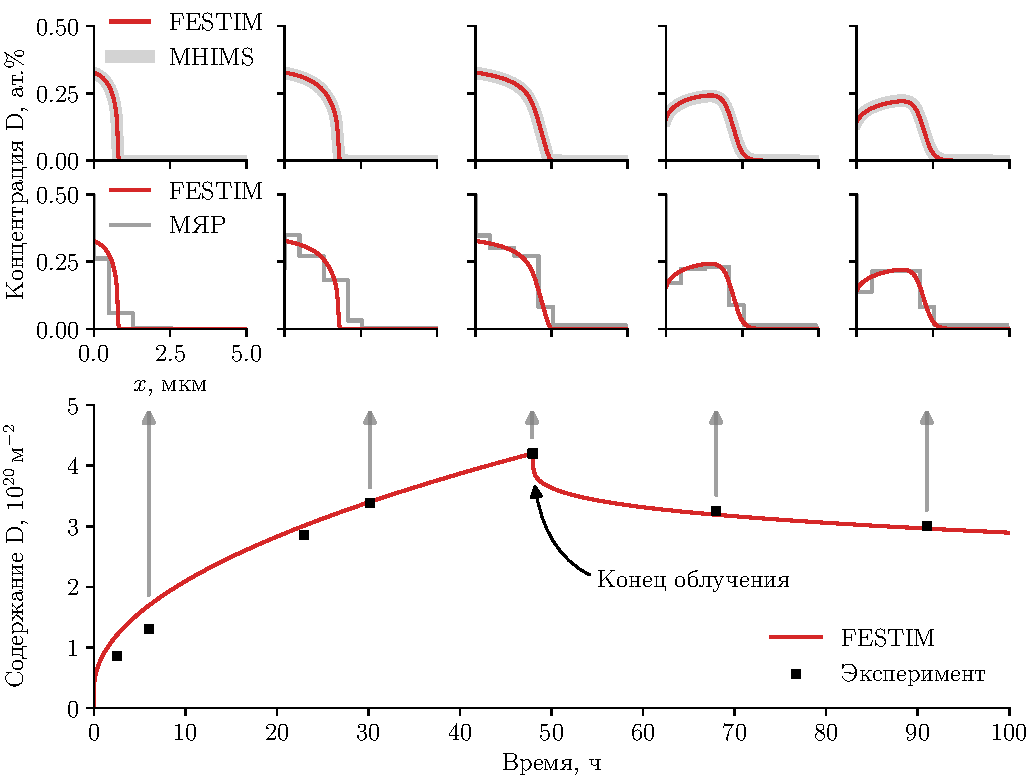
\includegraphics[scale=1]{val3.pdf}
    }
    \caption{Временная эволюция содержания дейтерия в вольфраме (внизу). Сравнение между данными FESTIM и МЯР (в середине) и между данными FESTIM и MHIMS (вверху)}\label{fig:ch2/val3}
\end{figure}

Во время фазы экспозиции содержание дейтерия увеличивается (см. нижний график на рис.~\ref{fig:ch2/val3}), профиль концентрации расширяется по мере заполнения более глубоколежащих дефектов (см. верхний/средний ряд графиков). Во время фазы десорбции наблюдается более медленное снижение накопления из-за наличия ловушек с высокой ($>$\SI{1.5}{\electronvolt}) энергией активации освобождения. Результаты, полученные в коде FESTIM, хорошо согласуются с экспериментальными данными (среднеквадратическое отклонение в величине интегрального накопления \SI{2.1e19}{\per\meter\squared}) и совпадают с данными MHIMS.

\subsubsection{Эксперимент по облучению стали EUROFER ионами дейтерия}
Последний валидационный тест посвящен накоплению дейтерия при облучении стали EUROFER ионами с низкой энергией~\cite{Schmid2023_1}. Эксперименты проводились с тремя типами образцов толщиной \(L=\SI{0.8}{\milli\meter}\): неповрежденными; предварительно поврежденными ионами вольфрама с энергией \SI{20}{\mega\electronvolt}; предварительно облученными дейтерием и затем поврежденными ионами вольфрама. Эти образцы облучались потоком дейтерия $\Gamma_\mathrm{D}\approx\SI{9e19}{\per\meter\squared\per\second}$ с энергией \SI{5}{\text{эВ/ион}} при давлении газа $p_\mathrm{D_2}=\SI{1}{\pascal}$ и температуре \SI{370}{K}. \fixme{При указанном давлении в камере поток атомов в составе тепловых молекул из газовой фазы сопоставим с потоком ионов, что указывает на необходимость явного учета кинетики процессов на поверхности.} Время облучения дейтерием в этих экспериментах варьировалось от \num{48} до \SI{143}{\hour}, что приводит к четырем модельным случаям:
\begin{enumerate}[beginpenalty=10000]
    \item Неповрежденный образец $\rightarrow$ облучение дейтерием длительностью \SI{143}{\hour}.
    \item Поврежденный образец $\rightarrow$ облучение дейтерием длительностью \SI{48}{\hour}.
    \item Поврежденный образец $\rightarrow$ облучение дейтерием длительностью \SI{143}{\hour}.
    \item Предоблученный дейтерием поврежденный образец $\rightarrow$ облучение дейтерием длительностью \SI{48}{\hour}.
\end{enumerate}
После облучения образцы хранились в течение \SI{24}{\hour} при \SI{290}{\kelvin}. Затем были проведены \textit{ex situ} ТДС-измерения со скоростью нагрева \SI{3}{\kelvin\per\minute} до температуры \SI{800}{\kelvin}. \fixme{Вынос образцов на атмосферу вносит неопределенность о состоянии поверхности, что существенно усложняет проведение моделирования. В оригинальной работе однако отмечается, что в ходе ТДС поток десорбированных частиц в основном состоял из молекул дейтерия, когда десорбция молекул, содержащих протий и кислород, была незначительной.}

Подобно предыдущему случаю моделирования, в кинетическую модель поверхности включены три механизма: диссоциативная адсорбция молекул ($J_\mathrm{ads}^{\mathrm{D_2}}$), рекомбинация молекул ($J_\mathrm{des}^{\mathrm{D_2}}$) и десорбция за счет мгновенной рекомбинации с приходящими ионами ($J_\mathrm{des}^{\mathrm{D}}$). Результирующая плотность потока атомов равна:
\begin{subequations}
    \label{eq:ch2/case4_Jvs}
    \begin{align}
        \Jvs                          & = J_\mathrm{ads}^{\mathrm{D_2}}-J_\mathrm{des}^{\mathrm{D_2}}-J_\mathrm{des}^{\mathrm{D}}, \\
        J_\mathrm{ads}^{\mathrm{D_2}} & = 2 \, \nu_\mathrm{ads}^{\mathrm{D_2}} p_\mathrm{D_2} \, \left( 1 - \theta \right)^2,      \\
        J_\mathrm{des}^{\mathrm{D_2}} & = 2 \, \nu_\mathrm{des}^{\mathrm{D_2}} \, \csurf^2,                                        \\
        J_\mathrm{des}^{\mathrm{D}}   & = \nu_\mathrm{des}^{\mathrm{D}} \, \csurf.
    \end{align}
\end{subequations}
Константа скорости адсорбции молекул рассчитывается как во втором и третьем валидационных тестах (уравнение~\cref{eq:ch2/nu_ads_P}). Константа скорости десорбции по каналу Или"--~Ридила определяется аналогично прошлому тесту, но на основе потока внедренных частиц: \( \Gamma_\mathrm{D}^{\mathrm{impl}}=\Gamma_\mathrm{D}(1-r) \), где \( r \) "--- коэффициент отражения частиц от поверхности.

Переход из растворенного в адсорбированное состояние полагается определяемым диффузией: $E_\mathrm{bs}=E_\mathrm{D}$ и $\nu_\mathrm{bs,0}=D_0/\lambda_\mathrm{IS}$. Количество межузельных и адсорбционных положений рассчитываются на основе концентрации атомов стали ($n_\mathrm{EFe}$). Константа скорости перехода из адсорбированного в растворенное состояние выбирается таким образом, чтобы выполнялся закон Сивертса:
\begin{flalign}
    \label{eq:ch2/case4_ksb}
    \nusb = \nubs \, K_\mathrm{S} \, \sqrt{\frac{\nu_\mathrm{des}^{\mathrm{D_2}}}{\nu_\mathrm{ads}^{\mathrm{D_2}}}}.
\end{flalign}

Во всех модельных случаях учитываются естественные центры захвата ($n_{\mathrm{t,1}}$) с равномерным распределением в объеме образца. Для поврежденных образцов добавляются индуцированные дефекты ($n_\mathrm{t,2}$) со следующим распределением в пределах поврежденной зоны:
\begin{equation}
    f(x)=0.5 \, \left( 1-\tanh \left( \frac{x-x_0}{\Delta x} \right)\right),
\end{equation}
где $x_0=\SI{3.3}{\micro\meter}$ и $\Delta x = \SI{0.01}{\micro\meter}$. Концентрация индуцированных центров захвата варьировалась в зависимости от присутствия дейтерия во время повреждения. Предполагается, что захват в каждый тип дефекта определяется диффузией.

В силу того, что левая поверхность ($x=0$) подвержена потоку ионов дейтерия, на ней рассматривается полная кинетическая модель поверхности. В расчетах также учитывается объемный источник подвижных атомов дейтерия вблизи открытой поверхности:
\begin{subequations}
    \label{eq:ch2/norm_impl_flux}
    \begin{align}
        S(x)       & = \Gamma_\mathrm{D}^{\mathrm{impl}} \varphi(x),                                      \\
        \varphi(x) & = \dfrac{N}{\sqrt{2\pi} \sigma} \, \exp \left( -\dfrac{(x-X)^2}{2\sigma^2}  \right), \\
        N          & = \dfrac{2}{1 + \erf \left( \dfrac{X}{\sqrt{2}\sigma} \right)},
    \end{align}
\end{subequations}
где \( \mathrm{erf}(x) \) "--- функция ошибок, \( X \) "--- глубина внедрения, \si{\meter}; \( \sigma \) "--- стандартное отклонение распределения. На правой границе ($x=L$) учитывается только десорбция за счет рекомбинации на поверхности. Моделирование проводилось на неоднородной сетке (шаг дискретизации меньше у левой границы), состоящей из 650 элементов, с нулевыми начальными условиями как для подвижного, так и для адсорбированного дейтерия. Список входных параметров указан в таблицах~\cref{tab:case4_inputs,tab:case4_traps_params}. На рисунке~\cref{fig:ch2/val4} приведено сравнение с результатами экспериментальных измерений и расчетов в коде TESSIM-X~\cite{Schmid2023_2}.

\nomenclature[P, 64]{\( r \)}{Коэффициент отражения частиц}
\nomenclature[P, 64]{\( X \)}{Глубина внедрения частиц, \si{\meter}}
\nomenclature[P, 64]{\( \sigma \)}{Стандартное октлонение профиля внедренных частиц, \si{\meter}}
\nomenclature[P, 64]{\( q \)}{Плотность потока тепла, \si{\watt\per\meter\squared}}

\begin{figure}[ht]
    \centerfloat{
        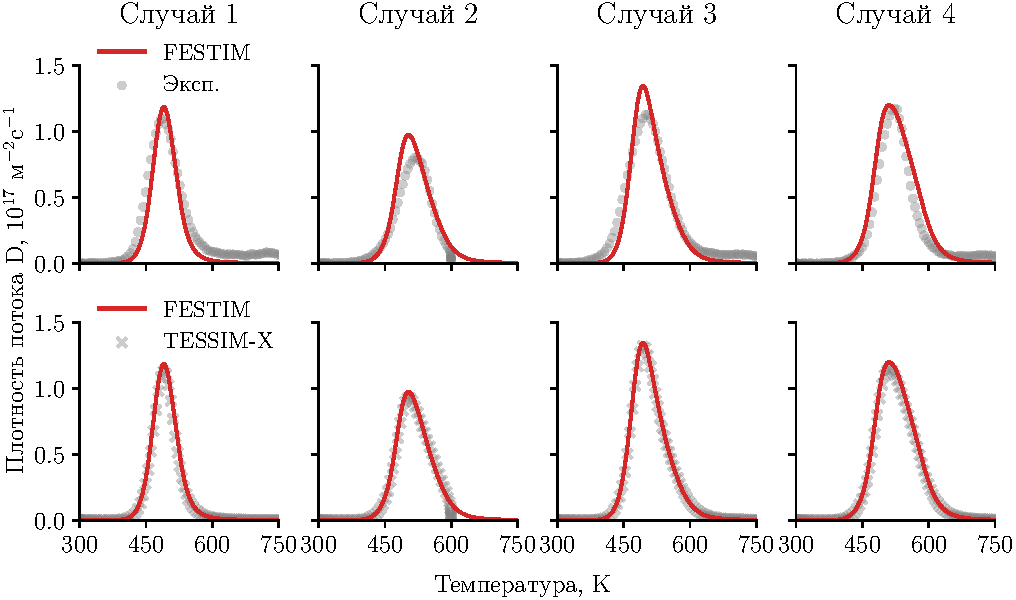
\includegraphics[scale=1]{val4.pdf}
    }
    \caption{ТДС-спектры дейтерия из разных образцов стали EUROFER. Сравнение с экспериментальными данными (вверху) и результатами моделирования в коде TESSIM-X (внизу)}\label{fig:ch2/val4}
\end{figure}

Наличие индуцированных центров захвата немного сдвигает основные пики ТДС-спектров в область более высоких температур. Их присутствие также приводит к уширению профиля, характеризующегося более плавно спадающим высокотемпературным плечом. Хотя согласие между результатами FESTIM и экспериментальными данными (верхний ряд на рис.~\ref{fig:ch2/val4}) является удовлетворительным (среднеквадратическое отклонение составляет \SI{7.9e15}{\per\meter\squared\per\second}), корреляция с TESSIM-X (нижний ряд на рисунке) гораздо лучше. Незначительные расхождения можно отнести к отличиям в реализациях модели, учитывающей процессы на поверхности, а также в некоторых входных параметрах, которые восстановить не удалось.

\section{Выводы к главе 2}

Программный пакет FESTIM является апробированным инструментом для моделирования транспорта изотопов водорода в материалах на основе модели Макнабба и Фостера. При определяющем участии автора в коде была реализована гибкая модель, которая позволяет явно учитывать эволюцию концентрации адсорбированного водорода за счет обратимых процессов перехода между растворенным и адсорбированным состояниями, а также различных каналов адсорбции и десорбции.

Возможности модели, учитывающей процессы на поверхности, были продемонстрированы успешным воспроизведением результатов четырех экспериментальных работ. Моделирование показало хорошее согласие с экспериментальными данными при различных предположениях относительно процессов в объеме и на поверхности, определяющих динамику водорода в материалах, что существенно расширяет область применения кода FESTIM. Верификация и высокая корреляция результатов с другими расчетными кодами (MHIMS и TESSIM-X), \fixme{разработанными независимыми исследовательскими группами, подтвердили аккуратность имплементации модели.}

\nomenclature[A, 13]{MMS}{Метод построенных решений (Method of manufactured solutions)}

\FloatBarrier
           % Глава 2
\chapter{Захват дейтерия в вольфраме под действием импульсно-периодических плазменных нагрузок}\label{ch:ch3}

В действующих токамаках наилучшие параметры удержания энергии в плазме достигаются в H"=моде, переход в которую сопровождается периодическим развитием краевых неустойчивостей (ELM-событий). Данные неустойчивости в основном возникают в области пьедестала и приводят к отрыву плазменных филаментов с их последующим попаданием в скреп-слой. Распространяясь вдоль силовых магнитных линий в скреп-слое, пламенные филаменты в итоге приходят на ОПЭ, вызывая мощное кратковременное (\( \leq \SI{1}{\milli\second} \)) облучение поверхности интенсивными потоками тепла и высокоэнергетичных частиц.

Анализ устойчивости вольфрама к мощным импульсно-периодическим нагрузкам проводился достаточно активно с целью определения допустимых рабочих условий и предельных ресурсных возможностей~\cite{Pintsuk2012,Budaev2015,Rieth2019}. С другой стороны, в главе~\cref{ch:ch2} было показано, что гораздо меньшее внимание было уделено вопросу накопления изотопов водорода под действием мощных потоков тепла и высокоэнергетичных частиц, соответствующих ELM-событиям. Немногочисленные эксперименты были проведены на линейных импульсных установках~\cite{Poskakalov2020,Ogorodnikova,Nishijima2011}, которые способны воспроизвести ожидаемую величину тепловых потоков во время ELM-событий в крупных токамаках, как ИТЭР, но при большей плотности потока (\(\sim\SI{e26}{\per\meter\squared\per\second}\)) и значительно меньшей энергии частиц (\(\sim\SI{10}{\electronvolt}\)). 

Данная глава посвящена анализу влияния импульсно-периодических плазменных нагрузок, соответствующих ELM-событиям в крупных токамаках, на длительное накопление дейтерия в вольфраме. Анализ был проведен на основе численного моделирования захвата дейтерия в вольфрамовых ОПЭ в условиях, ожидаемых в режиме плазменных разрядов с \(Q_\mathrm{fus}=\num{10}\) токамака ИТЭР~\cite{Kulagin2025_JNM}. Перед представлением основных результатов моделирования в данной главе проводится оценка применимости используемого подхода на основе сравнения с экспериментальными данными, полученными в экспериментах на КСПУ-Т~\cite{Poskakalov2020}. Все исходные коды в программном пакете FESTIM и результаты проведенных расчетов распространяются свободно~\cite{Kulagin_PhD_2025}.

\section{Моделирование захвата дейтерия при импульсном плазменном облучении в установке КСПУ-Т}\label{sec:ch3/sec1}
\subsection{Детали эксперимента}\label{sec:ch3/sec1/subsec1}
Эксперименты по исследованию накопления дейтерия при импульсном плазменном воздействии на КСПУ-Т проводились с поликристаллическими образцами вольфрама ($10\times13\times2$\,мм). Исследуемый образец помещался в композитную мишень (см. рисунок~\cref{fig:ch3/QSPA_target}), состоящую из двух частей: 8 одинаковых вольфрамовых элементов, окружающих центральный образец, и 4 внешних молибденовых пластины.
\begin{figure}[ht]
	\centerfloat{
		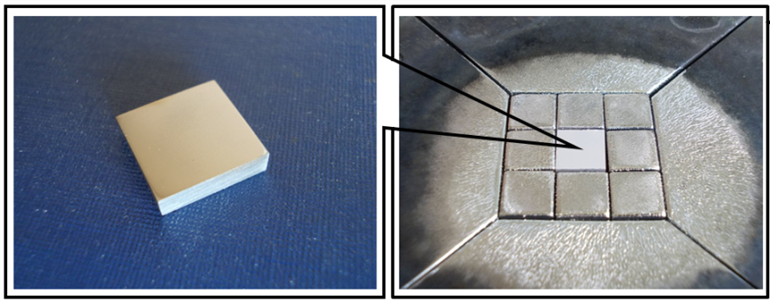
\includegraphics[scale=1]{QSPA_target.png}
	}
	\caption{Фотография образца вольфрама отдельно и в составе композитной мишени~\cite{Poskakalov2020}}\label{fig:ch3/QSPA_target}
\end{figure}
Композитная мишень помещалась в вакуумную камеру установки при остаточном давлении менее \SI{5e-3}{\pascal}. Образцы облучались импульсными потоками дейтериевой плазмы с длительностью около \SI{1}{\milli\second}. Характерный диаметр плазменного потока составил \SI{6}{\centi\meter}, что обеспечивало равномерное облучение центрального образца. Плотность поглощенной энергии измерялась предварительно с помощью калориметрической системы в зависимости от напряжения зарядки батареи ускорителя. 

В рамках экспериментов величина тепловых нагрузок варьировалась от \num{0.4} до \SI{3.7}{\mega\joule\per\meter\squared}, что позволило исследовать захват в двух режимах: без плавления (\( \lesssim \SI{1.4}{\mega\joule\per\meter\squared} \)) и с плавлением (\( \gtrsim \SI{1.4}{\mega\joule\per\meter\squared} \)). В рамках данного раздела будет рассмотрен только случай облучения при плотности поглощенной энергии равной \SI{0.7}{\mega\joule\per\meter\squared}, для которого представлено больше всего информации в оригинальной работе. Величина тепловой нагрузки соответствует напряжению зарядки конденсаторных батарей в \SIrange{1.6}{1.7}{\kilo\volt}. При таком напряжении скорость свободного потока дейтериевой плазмы на плато разряда составляет \(\approx \SI{40}{\kilo\meter\per\second} \), что соответствует \(\approx \SI{17}{\electronvolt} \) энергии направленного движения ионов~\cite{Yaroshevskaya2024}. Максимальная плотность потока частиц в ходе облучения была оценена на основе массового расхода рабочего газа и составила \( \Gamma_\mathrm{D}=\SI{7.5e26}{\per\meter\squared\per\second} \).

Образец вольфрама подвергался воздействию плазменного потока только один раз и охлаждался до комнатной температуры внутри установки за счет теплообмена с элементами мишени и излучения. На тыльной стороне мишени крепилась термопара, которая позволила фиксировать изменение температуры поверхности с разрешением в одну секунду. Содержание дейтерия определялось методом ТДС при скорости нагрева \SI{2}{\kelvin\per\second} после извлечения образца из вакуумной камеры и выноса на атмосферу. Идентичный образец, облученный при таких же параметрах плазменного импульса, был исследован с помощью МЯР для определения распределения захваченного дейтерия в приповерхностном слое.

\subsection{Расчетная модель}\label{sec:ch3/sec1/subsec2}
Моделирование захвата дейтерия при импульсном воздействии проводилось на основе численного решения уравнений~\cref{eq:ch2/mobile_conc,eq:ch2/heat_equation} в одномерном приближении (толщина области \( L=\SI{2}{\milli\meter} \)). Расчеты проводились в два этапа. Первый этап включал в себя фазы облучения (\(\sim \SI{1}{\milli\second}\)) и последующего хранения образца (\SI{e4}{\second}) до проведения ТДС-измерений. На данном этапе совместно решались задачи транспорта дейтерия и переноса тепла. Второй этап имитировал ТДС-эксперимент, в котором температура материала была однородна и линейно изменялась со временем.

Для решения задачи переноса тепла были использованы температурно-зависимые параметры вольфрама, определяемыми выражениями~\cref{eq:app/W_props}. Как в работе~\cite{Poskakalov2020}, полагалось, что временная зависимость теплового потока, приходящего на облучаемую поверхность, пропорциональна зависимости тока разряда, которая была аппроксимирована кусочно-гладкой функцией:
\begin{subequations}
	\label{eq:ch3/pulse_form}
	\begin{align}
		q(t) & =\frac{E_0}{\tau_\mathrm{imp}} \, w(t), \\
		w(t) & : \left\{
		\begin{alignedat}{2}
			w_1(t) & = 1 - \exp \left( -\frac{t}{\tau_\mathrm{le}} \right), & 0 \leq t \leq t_1, \\
			w_2(t) & = w_1(t) \, \left( 1 + \Delta \frac{t-t_1}{t_2 - t_1} \right), & \quad t_1 < t \leq t_2, \\
			w_3(t) & = w_2(t) \, \exp \left( -\frac{t-t_2}{\tau_\mathrm{te}} \right), & t > t_2,
		\end{alignedat}
		\right.
	\end{align}
\end{subequations}
где \( \tau_\mathrm{imp}=\int w(t')dt' \);  \( \tau_\mathrm{le}\) и \( \tau_\mathrm{te}\) "--- постоянные времени (измеряемые в секундах), характеризующие передний и задний фронты импульса; \( \Delta \) "--- постоянная, характеризующая нарастание (если положительна) или затухание (если отрицательна) импульса. Полученная временная зависимость представлена на рисунке~\cref{fig:ch3/QSPA_pulse}.
\begin{figure}[ht]
	\centerfloat{
		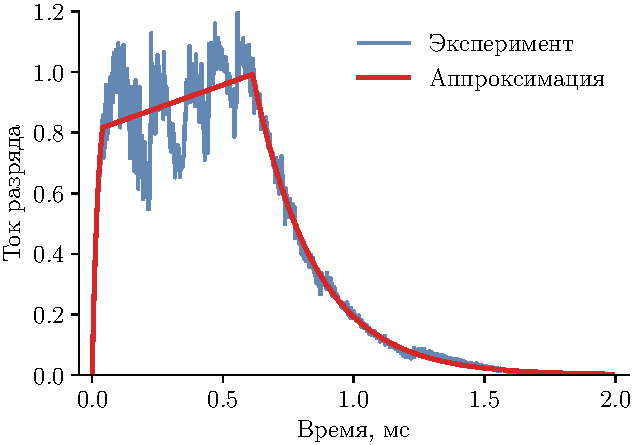
\includegraphics[scale=1]{QSPA_pulse.pdf}
	}
	\caption{Характерная временная зависимость тока разряда (условные единицы) в КСПУ-Т и ее аппроксимация кусочно-гладкой функцией}\label{fig:ch3/QSPA_pulse}
\end{figure}
На обеих границах расчетной области также задавались тепловые потери за счет излучения по закону Стефана-Больцмана с коэффициентом серости вольфрама \( \epsilon_\mathrm{W} \) равным \num{0.4}~\cite{weast1975crc}. Итоговое граничное условие (\( x=0 \)), определяющее нагрев материала выглядит следующим образом:
\begin{equation}
	-\kappa \left. \frac{\partial T}{\partial x} \right\vert_{x=0} = q(t) - \epsilon_\mathrm{W} \sigma_\mathrm{SB} (T^4-T_0^4),
\end{equation}
где \( \sigma_\mathrm{SB} = \SI{5.67e-8}{\watt\per\meter\squared\kelvin}^{4} \) "--- постоянная Стефана"--~Больцмана. На обратной поверхности учитывались только потери тепла за счет излучения. Расчет проводился на неоднородной сетке, состоящей из \num{2250} элементов (размер элементов вблизи левой границы был равен \SI{e-9}{\meter}), с использованием переменного временного шага для достижения большего временного разрешения в ходе импульса. Начальная температура была равна комнатной: \( T_0 = \SI{300}{\kelvin} \).

Первоначальный анализ решения однородного уравнения теплопроводности показал, что тыльная поверхность охлаждается гораздо медленнее, чем это наблюдалось в эксперименте (см. широкие линии на верхнем графике рисунка~\cref{fig:ch3/QSPA_T_ret}). Это вполне ожидаемо, так как в одномерном приближении не учитывается теплообмен с элементами мишени, окружающими центральный образец. Для воспроизведения экспериментальной эволюции температуры на правой границе уравнение теплопроводности было рассмотрено неоднородное уравнение теплопроводности со стоком мощности:
\begin{equation}
	\label{eq:ch3/QSPA_heat_transfer}
	\rho C_p \frac{\partial T}{ \partial t} = \frac{\partial}{\partial x}\left( \kappa \frac{\partial T}{\partial x} \right)  - k_\mathrm{loss} \kappa \left( T-T_0 \right),
\end{equation}
где \( k_\mathrm{loss}=\SI{1.2e3}{\per\meter\squared} \) "--- подгоночный коэффициент. Решение данного уравнения на обеих границах также приведено на рисунке~\cref{fig:ch3/QSPA_T_ret}. Эволюция температуры на левой границе во время плазменного импульса совпадает со случаем однородного уравнения, однако дальнейший спад на обеих поверхностях лучше согласуется с экспериментальными данными после первой секунды эксперимента.

\begin{figure}[ht]
	\centerfloat{
		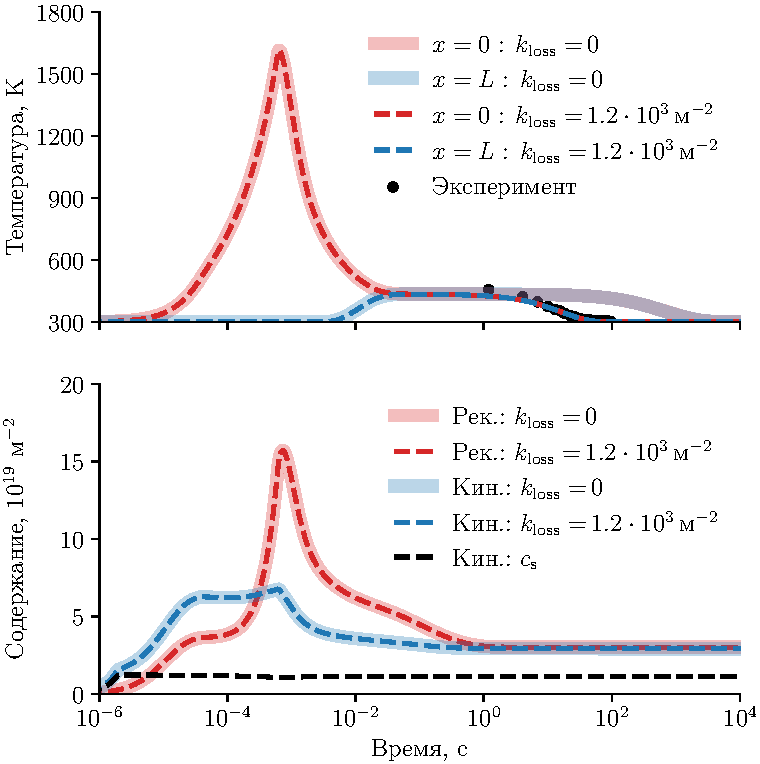
\includegraphics[scale=1]{QSPA_T_ret.pdf}
	}
	\caption{Верхний график: временные зависимости температуры на лицевой и тыльной сторонах образца для двух значений коэффициента, определяющего объемный сток тепла. Черные маркеры соответствуют экспериментальным данным~\cite{Poskakalov2020}; нижний график: временные зависимости интегрального содержания в образце при использовании коэффициента рекомбинации и полной модели, учитывающей кинетику процессов на поверхности. Пунктирной линией приведена временная зависимость концентрации адсорбированных атомов, рассчитанная в рамках второго подхода }\label{fig:ch3/QSPA_T_ret}
\end{figure}

Рассматривалась одномерная задача транспорта дейтерия в вольфраме:

\begin{equation}
	\label{eq:ch3/QSPA_diffusion}
	\frac{\partial \cm}{\partial x} = \frac{\partial }{\partial x} \left( D \left[ \frac{\partial \cm}{\partial x} + \frac{\cm Q^*}{\kBT^2} \frac{\partial T}{\partial x} \right] \right) - \sum\limits_i \frac{\partial \cti}{\partial t} + \Gamma_\mathrm{D} (1-r) \varphi(x),
\end{equation}
где источник подвижных атомов за счет имплантации задавался на основе нормированного распределения Гаусса:
\begin{subequations}
	\label{eq:ch3/norm_impl_flux}
	\begin{align}
		\varphi(x) & = \dfrac{N}{\sqrt{2\pi} \sigma} \, \exp \left( -\dfrac{(x-X)^2}{2\sigma^2}  \right),                         
	\end{align} 	
	\begin{align}
		N          & = \dfrac{2}{\erf \left( \dfrac{L-X}{\sqrt{2}\sigma} \right) + \erf \left( \dfrac{X}{\sqrt{2}\sigma} \right)}.
	\end{align}
\end{subequations}
Коэффициент отражения и параметры профиля имплантированных ионов определялись на основе расчетов в коде SDTrimSP~\cite{mutzke2024sdtrimsp}: \(r=0.78\); \(X=\SI{1.46e-9}{\meter} \); \(\sigma=\SI{0.81e-9}{\meter}\). Коэффициент диффузии определялся уравнением~\cref{eq:ch2/fernandez_diffusivity}, теплота переноса "--- в соответствии с уравнением~\cref{eq:ch1/heat_transport}. Сперва был проведен расчет, повторяющий оригинальную работу~\cite{Poskakalov2020}, где рассматривалось приближение равновесия на поверхности, при котором выход дейтерия определяется рекомбинацией с коэффициентом Пика и Сонненберга (выражение~\cref{eq:ch1/Kr_PS}). На правой границе задавалась нулевая концентрация подвижных атомов. Был использован один тип центров захвата с барьером выхода \( E_\mathrm{dt}=\SI{1.5}{\electronvolt} \), равномерно распределенный по объему образца. Концентрация дефектов была выбрана равной \SI{e-3}{\text{ат.}\percent} в соответствии с данными МЯР.

С целью получения лучшего согласия с результатами ТДС-измерений был также рассмотрен случай наличия двух типов дефектов в материале с равномерным распределением по объему и суммарной концентраций равной \SI{e-3}{\text{ат.}\percent}. В обоих подходах временная эволюция неподвижных атомов дейтерия определялась на основе уравнения~\cref{eq:ch2/trapped_conc}. На левой границе задавалась полная модель (выражение~\cref{eq:ch2/adsorbed_conc}), описывающая кинетику процессов на поверхности. В рамках модели учитывалась только десорбция молекул (уравнения \cref{eq:ch2/molecular_desortion, eq:ch2/nu_des_mol_s}) при энергии активации процесса, определяемой уравнением~\cref{eq:ch2/Edes_coverage}. Параметры центров захвата дейтерия и функциональной зависимости барьера десорбции были определены путем автоматической оптимизации параметров~\cite{Delaporte-Mathurin2021}. Начальная концентрация дейтерия в обоих случаях моделирования полагалась равной нулю. Параметры расчетов, не представленные в настоящем разделе, обобщены в таблице~\cref{tab:W_props}.

На нижнем графике рисунка~\cref{fig:ch3/QSPA_T_ret} приведены временные зависимости интегрального содержания дейтерия в образце, рассчитанные в рамках двух предположений о протекании процессов на поверхности и двух значений коэффициента, определяющего объемный сток тепла. Можно заметить, что для обоих типов граничных условий влияния диссипативного слагаемого в уравнении теплопроводности не наблюдается, так как все процессы достигают равновесия за время \( \approx \SI{1}{\second} \). Примечательно, что содержание в обоих случаях оказывается приблизительно равным. Существенное отличие наблюдается во временной эволюции содержания, определяемой процессами на облучаемой поверхности. При учете эволюции концентрации адсорбированных атомов значительная часть дейтерия остается на поверхности.

\subsection{Сравнение результатов моделирования и эксперимента}\label{sec:ch3/sec1/subsec3}
Сравнение результатов расчетов в коде FESTIM и оригинальных результатов работы~\cite{Poskakalov2020} приведено на рисунке~\cref{fig:ch3/QSPA_TDS}. На левом графике приведены расчетные данные в приближении равновесия процессов на поверхности. Учитывая отличия в параметрах моделирования (коэффициент диффузии, константа скорости захвата в дефекты и т.д.) предыдущие результаты расчетов в коде TMAP7 удалось воспроизвести с энергией активации хемосорбции \(E_\mathrm{c}=\SI{0.83}{\electronvolt} \), что отличается от значения в оригинальной работе на \SI{0.1}{\electronvolt}. Численные результаты в обоих случаях не воспроизводят все особенности экспериментального ТДС-спектра, но дают представление о том, какие типы дефектов вносят основной вклад в условиях импульсного плазменного облучения.
\begin{figure}[ht]
	\centerfloat{
		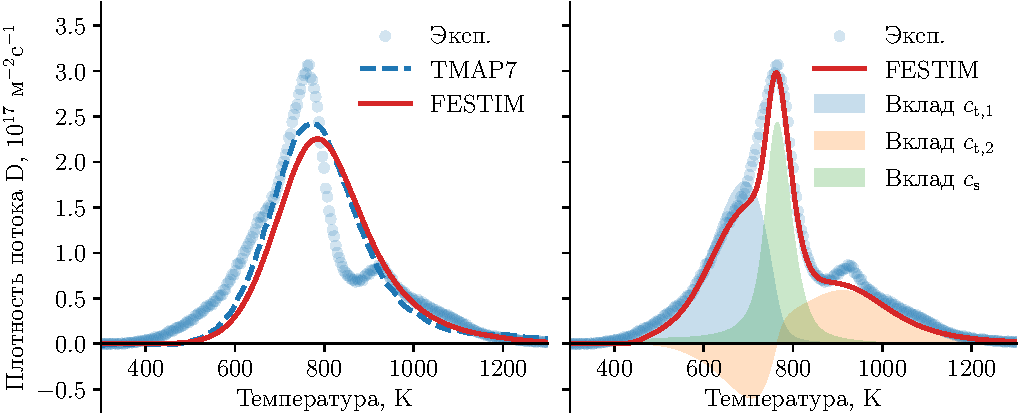
\includegraphics[scale=1]{QSPA_TDS.pdf}
	}
	\caption{Сравнение ТДС-спектров дейтерия из вольфрама, рассчитанных в коде FESTIM при двух предположениях о протекании процессов на поверхности, с данными, полученными в эксперименте и рассчитанными ранее в коде TMAP7~\cite{Poskakalov2020}}\label{fig:ch3/QSPA_TDS}
\end{figure}

Лучшее согласие было получено при явном учете процессов на поверхности с барьером десорбции, зависящем от концентрации атомов на поверхности. В ходе оптимизации были определены параметры центров дефектов: \(E_\mathrm{dt,1}=\SI{1.41}{\electronvolt}\), \(E_\mathrm{dt,2}=\SI{1.86}{\electronvolt}\), \(n_\mathrm{t,1}=\SI{0.79e-3}{\text{ат.\percent}}\) и \(n_\mathrm{t,2}=\SI{0.21e-3}{\text{ат.\percent}}\). Энергетический барьер выхода из дефектов первого типа близок к использованному в предыдущем случае (\SI{1.5}{\electronvolt}). Эти дефекты также можно связать с захватом в моновакансии, когда второй тип можно отнести к захвату в вакансионных кластерах. Также были получены параметры, определяющие зависимость барьера десорбции от концентрации атомов на поверхности (уравнение~\ref{eq:ch2/Edes_coverage}): \( E_\mathrm{c}=0 \), \( E_0 = 0 \), \( \Delta E = \SI{2.124}{\electronvolt} \), \( \theta_0 = \num{0.580} \) и \( \delta\theta=\num{0.026} \).

Вклад в поток десорбированных частиц от каждого типа атомов проиллюстрирован на правом графике рисунка~\cref{fig:ch3/QSPA_TDS}. Вклад от захваченных в дефекты атомов качественно определяется как изменение их интегральной концентрации, взятое со знаком минус (вклад в поток десорбированных частиц положителен при выходе атомов из дефектов и отрицателен при обратном захвате). Вклад от концентрации адсорбированных атомов, определяется ее производной по времени, взятой со знаком минус. Из сравнения можно заметить, что основной пик спектра воспроизводится за счет эволюции концентрации адсорбированных атомов, когда начало левого плеча и правое плечо спектра определяются взаимодействием с дефектами. В рамках данного эксперимента учет концентрации атомов на поверхности может быть необходим в виду того, что доза захваченного дейтерия сравнительно мала. При насыщении поверхности концентрация адсорбированных атомов составит \( \approx \SI{2e19}{\per\meter\squared} \), что соизмеримо с измеренным содержания дейтерия \( \approx \SI{3e19}{\per\meter\squared}\).

В рамках обоих предположений о протекании процессов вблизи поверхности было получено косвенное подтверждение ограниченной скорости выхода дейтерия (наличие большого барьера для десорбции) после импульсного облучения. Однако фактическая подгонка спектра не позволяет сделать однозначные выводы о природе полученного спектра. При интенсивном облучении с высоким потоком атомов, как в КСПУ-Т, возможно образование полей напряжений и дефектов вблизи поверхности, которые будут препятствовать выходу дейтерия из образца. Важно также отметить, что в обоих модельных случаях глубина проникновения дейтерия за один импульс составляет десятки микрометров (см. рисунок~\cref{fig:ch3/QSPA_conc}). Большая подвижность в приповерхностном слое определяется достижением высоких температур при импульсном плазменном нагреве.
\begin{figure}[ht]
	\centerfloat{
		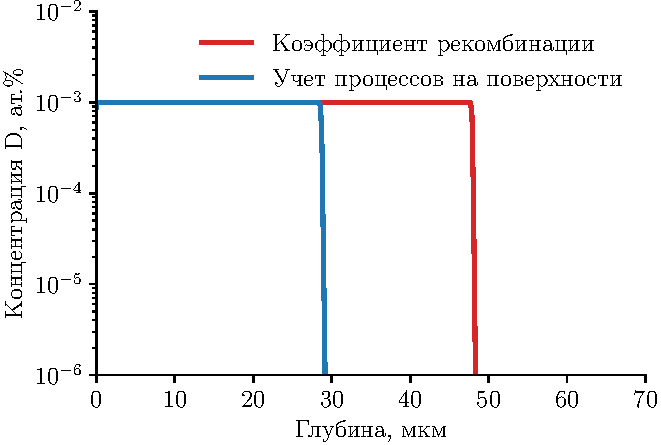
\includegraphics[scale=1]{QSPA_conc.pdf}
	}
	\caption{Рассчитанные распределения концентрации дейтерия в вольфраме после стадии хранения образца при двух предположениях о протекании процессов на поверхности}\label{fig:ch3/QSPA_conc}
\end{figure}

Таким образом, численные расчеты с использованием описанных в главе~\cref{ch:ch2} моделей позволяет добиться разумного согласия с экспериментальными данными, полученными на КСПУ-Т. Необходимо, однако, подчеркнуть, что более точный анализ возможен при проведении дополнительных экспериментальных измерений, которые могли бы позволить сократить число свободных параметров.

\section{Моделирование накопления дейтерия в вольфраме под действием импульсно"=периодических плазменных нагрузок}\label{sec:ch3/sec2}
Описанные экспериментальные условия в плазменном ускорителе КСПУ-Т не воспроизводят всех особенностей облучения, ожидаемых в крупных установках с магнитным удержанием плазмы. В силу этого, результаты предыдущего раздела нельзя напрямую экстраполировать на случай облучения ОПЭ в токамаках, но они иллюстрируют применимость используемых подходов к анализу накопления изотопов водорода при импульсном воздействии. В данном разделе проводится численное моделирование накопления дейтерия в условиях, приближенных к случаю облучения ОПЭ в диверторе ИТЭР во время ELM"=событий.

\subsection{Постановка задачи}
Дивертор токамака ИТЭР будет изготовлен из композитных моноблоков, состоящих из слоя вольфрама (W) с минимальной толщиной \SIrange{6}{8}{\milli\meter}, цилиндрической медной (Cu) прослойки с толщиной \SI{1}{\milli\meter} и охлаждающей трубки из сплава бронзы (CuCrZr) с внутренним диаметром \SI{12}{\milli\meter} и толщиной \SI{1.5}{\milli\meter} (см. рисунок~\cref{fig:ch3/ITER_monoblock}). Для качественного анализа влияния переходных событий на удержание дейтерия было рассмотрено одномерное приближении самой тонкой области моноблока между обращенной к плазме и охлаждаемой водой сторонами (выделена красной линией на оси симметрии на рисунке~\cref{fig:ch3/ITER_monoblock}). Итоговая геометрическая модель также показана на рисунке~\cref{fig:ch3/ITER_monoblock} и включает слой вольфрама толщиной \SI{6}{\milli\meter}, миллиметровый слой меди и полуторамиллиметровый слой сплава бронзы.

\begin{figure}[ht]
	\centering
	\begin{overpic}[scale=1]
		{ITER_monoblock.pdf}
		%\put(6, 75){ \textbf{(а)}}
		%\put(56.5, 75){ \textbf{(б)}}
		\put(74.2, 61.2){ $S_{\mathrm{ELM}}$}
		\put(71.2, 65.2){ $S_{\mathrm{stat}}$}
		\put(24.7, 77.4){$q_{\mathrm{heat}}$}
		\put(74.0, 77.4){$q_{\mathrm{heat}}$}
		\put(74.0, 5.2){$q_{\mathrm{loss}}$}
		\put(58.3, 40.4){$x$}
	\end{overpic}
	\caption{Полоидальное сечение диверторного моноблока ИТЭР (слева) и одномерное представление кратчайшего расстояния от облучаемой до водоохлаждаемой поверхности, соответствующее красной линии на левом рисунке. Размеры указаны в мм. \cruleme[customgrey]{0.5cm}{0.5cm}~---~W; \cruleme[customorange]{0.5cm}{0.5cm} "--- Cu; \cruleme[customyellow]{0.5cm}{0.5cm} "--- CuCrZr. }\label{fig:ch3/ITER_monoblock}
\end{figure}

Этот подход использовался в недавнем исследовании~\cite{Dasgupta2023} влияния эффекта Соре на удержание легких атомов в вольфраме при тепловых нагрузках (без учета изменения потока частиц), соответствующих ELM"=событиям. На основе расчетов эволюции температуры было показано, что приближение качественно соответствует двумерному моделированию нагрева поверхности вольфрама~\cite{VandenKerkhof2021}. Однако тороидальное (горизонтальное на рисунках) распределение температуры по глубине моноблока может отклоняться от равномерного в зависимости от условий облучения~\cite{Delaporte-Mathurin2020, Delaporte-Mathurin2023}. Такой профиль температуры соответственно приведет к неоднородному пространственному распределению захваченных изотопов водорода в моноблоке. Принципиальным ограничением рассмотрения упрощенной геометрии (1D "--- 2D) также является невозможность учета влияния эффектов на свободных поверхностях (охлаждение за счет излучения, десорбция). Данные упрощения, очевидно, не позволяют проводить точные количественные оценки содержания, но не должны влиять на качественные закономерности накопления.

Изменение температуры вдоль упрощенной геометрии было получено с помощью однородного одномерного уравнения теплопроводности в приближении идеального теплового контакта на границах раздела материалов (аналогично уравнению~\cref{eq:ch3/QSPA_heat_transfer} без учета диссипативного слагаемого). Температурные зависимости физических свойств материалов приведены в приложении~\cref{app:A}. Полагалось, что нагрев материала определяется стационарными потоками тепла (\( q_\mathrm{stat} \)), приходящими на поверхность вольфрама на протяжении всего облучения, импульсно-периодическими потоками тепла во время ELM"=событий (\( q_\mathrm{ELM} \)) и излучением:
\begin{equation}
	\label{eq:ch3/left_BC_ITER}
	\left.-\kappa\frac{\partial T}{\partial x}\right\vert_{x=0}=q_{\mathrm{stat}}+q_{\mathrm{ELM}}(t)-\epsilon_{\mathrm{W}}\sigma_\mathrm{SB}(T^4-T_0^4),
\end{equation}
где температура окружающей среды, как и начальная, полагалась равной комнатной (\SI{300}{\kelvin}). Коэффициент серости вольфрама выбран равным 0,4~\cite{weast1975crc}. На обратной границе геометрической области были заданы потери тепла за счет водяного охлаждения:
\begin{equation}
	\label{eq:ch3/right_BC_ITER}
	\left.-\kappa\frac{\partial T}{\partial x}\right\vert_{x=L}=q_{\mathrm{loss}}(T),
\end{equation}
где \( L=\SI{8.5}{\milli\meter} \) "--- полная длина геометрической области. Зависимость тепловых потерь от температуры со стороны охлаждающей жидкости задавалось с помощью линейной интерполяции данных, представленных Маршаллом и др.~\cite{Marshall2001} на основе спецификации ИТЭР~\cite{komarov2013thermal}.

Моделирование транспорта дейтерия в композитной геометрии требует обеспечения непрерывности химического потенциала на границе раздела материалов~\cite{Delaporte-Mathurin2021_3}. Для упрощения анализа моделирование проводилось только для вольфрамового слоя толщиной \( L_\mathrm{W}=\SI{6}{\milli\meter} \). На таких временных масштабах, когда дейтерий не достигает границы раздела W-Cu, полученные результаты будут воспроизводить результаты для композитной геометрии. Согласно предыдущим расчетам~\cite{Delaporte-Mathurin2019, Delaporte-Mathurin2021_3}, достижение границы раздела происходит за тысячи секунд (десятки плазменных циклов, подобных ИТЭР). Учитывая это, плазменное облучение в настоящих расчетах было ограничено случаем \SI{1000}{\second}, что соответствует \( \approx \SIrange{2.0}{2.5}{} \) разрядам в ИТЭР. Чтобы сохранить распределение температуры неизменным по сравнению со случаем композитной геометрии, температурные зависимости теплового потока, протекающего через границу раздела W-Cu, были параметризованы в зависимости от условий облучения. Полученные зависимости затем задавались на задней поверхности вольфрама в качестве граничного условия. Обоснование данного приближения приводится в разделе~\cref{subsec:ch3/sec2/subsec3}.

В задаче транспорта учитывались два источника атомов, внедряемых в объем во время стационарных (\( S_\mathrm{stat} \)) и импульсно-периодических нагрузок (\( S_\mathrm{ELM} \)). Рассматривался один тип центров захвата, равномерно распределенный в образце с концентрацией (\( n_\mathrm{t} \)) и барьером освобождения \(E_\mathrm{dt} \).
\begin{subequations}
	\label{eq:ch3/diffusion_equation_ITER}
	\begin{align}
		\dfrac{\partial c_{\mathrm{m}}}{\partial t} & =-\dfrac{\partial J_x}{\partial x} - \dfrac{\partial c_{\mathrm{t}}}{\partial t} + S_{\mathrm{stat}}(x)+S_{\mathrm{ELM}}(x,t),
	\end{align}
\end{subequations}
где диффузионный поток вдоль оси \( x \) определяется градиентами концентрации и температуры (см. уравнение~\cref{eq:ch3/QSPA_diffusion}). Объемные источники задавались аналогично уравнениям~\cref{eq:ch3/norm_impl_flux}. Параметры, характеризующие их пространственное распределение, были получены в коде SDTrimSP~\cite{mutzke2024sdtrimsp} в зависимости от энергии приходящих частиц. Временная эволюция захваченных в дефекты атомов определялась из уравнения~\cref{eq:ch2/trapped_conc}. 

Для анализа влияния свойств центров захвата на удержание дейтерия барьер выхода из них варьировался в диапазоне от \num{1} до \SI{2}{\electronvolt} при фиксированной концентрации дефектов \SI{e-2}{\text{ат.}\percent}, в то время как концентрация дефектов "--- в диапазоне от \num{e-3} до \SI{1}{\text{ат.}\percent} при барьере выхода \SI{1.5}{\electronvolt}. В иных случаях $E_{\mathrm{dt}}=\SI{1.5}{\electronvolt}$ и $n_{\mathrm{t}}=\SI{e-2}{\text{ат.}\percent}$ использовались в качестве базовой комбинации параметров, которую можно отнести к естественной концентрации дефектов вакансионного типа в вольфраме~\cite{DeTemmerman2018}. Параметры, определяющие транспорт дейтерия, обобщены в таблице~\cref{tab:W_props}. Теплота переноса задавалась на основе уравнения~\cref{eq:ch1/heat_transport}. Расчетная геометрия была дискретизирована с использованием неоднородной сетки из 750 элементов, в которой положение узлов определялось на основе геометрической прогрессии:
\[
	\forall n\in(0,750):\,x_{n}=x_{n-1}+\Delta x\,b^{n-1},
\]
где $\Delta x=\SI{0.1}{\nano\meter}$ и $b=1,0188$. Был использован переменный временной шаг, не превышающей величины \SI{50}{\micro\second}.

В качестве граничных условий в базовом сценарии моделирования задавалась нулевая концентрация подвижных атомов на обеих поверхностях. На основе результатов, полученных в ходе моделирования экспериментов в КСПУ-Т, а также учитывая особенности экспериментальной методики (например, вынос образцов на атмосферу), нельзя сделать однозначных выводов о влиянии процессов на поверхности. Для оценки роли скорости рекомбинации на поверхности в настоящей работе рассматривался случай конечной скорости рекомбинации, определяемой коэффициентом Пика и Сонненберга (уравнение~\cref{eq:ch1/Kr_PS}) с барьером активации хемосорбции \( E_\mathrm{c} \), варьируемым в диапазоне от \num{0.00} до \SI{0.83}{\electronvolt}.

\subsection{Параметры потоков тепла и частиц}
Влияние ELM-событий на накопление в вольфраме рассматривалось для трех модельных сценариев. Параметры потоков тепла и частиц были определены в соответствии с расчетами в коде SOLPS для базового режима ИТЭР при $Q_\mathrm{fus}=\num{10}$ (\SI{15}{\mega\ampere}/\SI{5.3}{\tesla}), хотя и предполагая дейтериевую плазму~\cite{Pitts2019, Orrico2023}. Основное внимание уделяется условиям облучения, ожидаемым на внешней мишени дивертора. В следующем подразделе будет дополнительно подчеркнуто, что используемые приближение для параметров нагрузок во время ELM-событий также справедливы для внешней мишени дивертора. Стационарные тепловые нагрузки были выбраны равными 1; 5 и \SI{10}{\mega\watt\per\meter\squared}. Согласно моделированию SOLPS~\cite{Pitts2019, Orrico2023}, такие тепловые потоки можно ожидать вблизи точки удара (strike-point) в режимах без или с частичным отрывом (partial detachment) плазмы дивертора.

Стационарный поток частиц для каждого сценария выражается через плотность тепловой мощности и электронную температуру на мишени дивертора ($T_{\mathrm{e,t}}$ в \si{\electronvolt}), предполагая равновесие между ионными и электронными компонентами плазмы~\cite{Brida2017, Stangeby2000}:
\begin{subequations}
	\label{eq:ch3/particle_flux_link}
	\begin{align}
		\Gamma_{\mathrm{stat}} & =\frac{q_{\mathrm{stat}}}{\gamma T_{\mathrm{e,t}} + E_{\mathrm{rec}}}, \\
		\gamma                 & =4.85\,(1-r_{\mathrm{stat}}^{\mathrm{E}})+2.15,
	\end{align}
\end{subequations}
где $\gamma$ "--- коэффициент пропорциональности (sheath heat transmission factor), учитывающий изменение энергии частиц при прохождении пристеночного слоя и снижение доли принесенной энергии при отражении частиц; $r_{\mathrm{stat}}^{\mathrm{E}}$ "--- коэффициент отражения энергии низкоэнергетичных ионов; $E_{\mathrm{rec}}=\SI{13.6}{\electronvolt}$ "--- энергия, выделяемая на мишени при нейтрализации ионов. Численные значения в уравнении~\cref{eq:ch3/particle_flux_link} получены для ионов дейтерия. Кинетическая энергия ионов дейтерия на мишени приблизительно равна~\cite{Brida2017}:
\begin{equation}
	\label{eq:ch3/stat_energy}
	E_{\mathrm{stat}}\approx 4.85\, T_{\mathrm{e,t}}.
\end{equation}

Для получения значений потоков дейтерия и их энергии температуры электронов на мишени были выбраны равными \num{10.5}; \num{15.5} и \SI{20.0}{\electronvolt}, что согласуется с результатами моделирования пристеночной плазмы в ИТЭР~\cite{Pitts2019, Orrico2023}. Параметры стационарных нагрузок обобщены в таблице~\ref{tab:stat_exposure} и близки к тем, которые применялись в других работах по моделированию накопления водорода в элементах дивертора ИТЭР~\cite{Delaporte-Mathurin2019, Delaporte-Mathurin2021_3, Delaporte-Mathurin2020, Delaporte-Mathurin2023, Hodille2021_2}.
\begin{table}[ht]
	\centering
	\caption{Параметры стационарных потоков тепла и частиц} \label{tab:stat_exposure}
	\begin{threeparttable}
		\renewcommand{\arraystretch}{1.2}%% Увеличение расстояния между рядами, для улучшения восприятия.
		\begin{tabularx}{\linewidth}{>{\centering\arraybackslash}X>{\centering\arraybackslash}X>{\centering\arraybackslash}X>{\centering\arraybackslash}X>{\centering\arraybackslash}X>{\centering\arraybackslash}X>{\centering\arraybackslash}Xc}
			\toprule
			$q_{\mathrm{stat}}$,
			   & $T_{\mathrm{e,t}}$,
			   & $\Gamma_{\mathrm{stat}}$,
			   & $E_{\mathrm{stat}}$,
			   & $r_{\mathrm{stat}}$
			   & $r_{\mathrm{stat}}^{\mathrm{E}}$
			   & $X_{\mathrm{stat}}$,
			   & $\sigma_{\mathrm{stat}}$,                                                                                             \\
			\si{\mega\watt\per\meter\squared}
			   & \si{\electronvolt}
			   & \SI{e23}{\per\meter\squared\per\second}
			   & \si{\electronvolt}
			   &
			   &
			   & \si{\nano\meter}
			   & \si{\nano\meter}                                                                                                      \\
			\hline
			\hline
			1  & \num{1.0}                               & \num{10.5} & \num{51} & \num{0.685} & \num{0.484} & \num{2.64} & \num{1.42} \\
			5  & \num{3.6}                               & \num{15.5} & \num{75} & \num{0.666} & \num{0.461} & \num{3.27} & \num{1.76} \\
			10 & \num{5.7}                               & \num{20.0} & \num{97} & \num{0.654} & \num{0.447} & \num{3.76} & \num{2.03} \\
			\bottomrule
		\end{tabularx}
	\end{threeparttable}
\end{table}

К настоящему времени разработано несколько моделей, позволяющих моделировать нагрузки на ОПЭ во время ELM-событий и исследовать соответствующие процессы взаимодействия~\cite{Krieger2025,Leonard2014,zohm1996edge}. Доминирующая часть из них требует проведения ресурсоемких расчетов динамики пристеночной плазмы, что затрудняет проведение анализа в широком диапазоне параметров. Упростить задачу можно с помощью модели <<свободного потока>> (FSM " --- free streaming model). В рамках модели ELM-событие рассматривается как отрыв плазменного филамента от области пьедестала с последующим его попаданием в скреп-слой. В приближении квазинейтральности решается одномерное уравнение Власова-Пуассона для бесстолкновительного адиабатического расширения этого филамента. Полученное решение позволяет определить временные зависимости потоков тепла и частиц в процессе таких событий~\cite{Fundamenski2006, Moulton2013}. Данная модель широко применялась для оценки общей эрозии ОПЭ~\cite{Abrams2018, Wang2024}, накопления легких ионов~\cite{Dasgupta2023} и поведения ОПЭ под действием тепловых нагрузок~\cite{VandenKerkhof2021} во время ELM-событий в токамаках.

Временные зависимости плотности потоков тепла (\( q_\mathrm{ELM} \)) и частиц (\( \Gamma_\mathrm{ELM} \)) в рамках FSM определены следующим образом:
\begin{subequations}
	\label{eq:ch3/elm_fluxes}
	\begin{align}
		\frac{q_{\mathrm{ELM}}(t)}{q_{\mathrm{ELM,0}}}           & =\left(1+\left(\frac{\tau}{t}\right)^2\right)\left(\frac{\tau}{t}\right)^2\exp\left(-\left(\frac{\tau}{t}\right)^2\right),\label{eq:elm_heat_flux} \\
		\frac{\Gamma_{\mathrm{ELM}}(t)}{\Gamma_{\mathrm{ELM,0}}} & =\left(\frac{\tau}{t}\right)^2\exp\left(-\left(\frac{\tau}{t}\right)^2\right), \label{eq:elm_part_flux}
	\end{align}
\end{subequations}
где $\tau=\num{0.8}\tau_{\mathrm{IR}}$; $\tau_{\mathrm{IR}}=$~\SI{250}{\micro\second} является постоянной времени фазы нарастания~\cite{Eich2017}. В соответствии с подходом, описанным в~\cite{VandenKerkhof2021}, нормировка теплового потока проводится на основе плотности потока энергии в плазменном филаменте, уносимой вдоль магнитных линий ($\varepsilon_\parallel$ в \si{\joule\per\meter\squared}):
\begin{equation}
	\label{eq:ch3/norm_elm_hf}
	\varepsilon_\parallel=\sin^{-1}(\alpha)\,\int\limits_{\tau_{\mathrm{ELM}}}q_{\mathrm{ELM}}(t)dt,
\end{equation}
где $\tau_{\mathrm{ELM}}$ "--- период повторения ELM-событий, с; $\alpha=4.2^{\circ}$ "--- полный угол наклона магнитных линий к поверхности мишени~\cite{Pitts2019, Eich2017, Pitts2017}. Плотность потока энергии на внешней мишени оценивается с помощью скейлинга Эйха и др.~\cite{Eich2017}, полученного путем обработки массива данных на внешней мишени диверторов современных токамаков во время ELM-событий первого типа:
\begin{equation}
	\label{eq:ch3/parallel_elm_fluence}
	\varepsilon_\parallel=0.28\times n_{\mathrm{e,ped}}^{0.75}\, T_{\mathrm{e,ped}}^{0.98}\, \delta_{\mathrm{ELM}}^{0.52}\, R_{\mathrm{geo}}^{1},
\end{equation}
где $\varepsilon_\parallel$ выражена в \si{\mega\joule\per\meter\squared}; $n_{\mathrm{e,ped}}$ "--- электронная плотность в области пьедестала, \SI{e20}{\per\meter\cubed}; $T_{\mathrm{e,ped}}$ "--- электронная температура в области пьедестала, \si{\kilo\electronvolt}; $\delta_{\mathrm{ELM}}=\Delta W_{\mathrm{ELM}}/W_{\mathrm{plasma}}$ "--- потери энергии в ходе ELM-событий относительно запасенной энергии в плазме, \si{\percent}; $R_{\mathrm{geo}}$ "--- большой радиус установки, \si{\meter}. Потери энергии в ходе ELM-событий определяются эмпирическим соотношением~\cite{Loarte2002} на основе мощности плазмы, в скреп-слое ($P_{\mathrm{SOL}}$~в~\si{\watt}):
\begin{equation}
	\Delta W_{\mathrm{ELM}} f_{\mathrm{ELM}}=0.3\pm 0.1 \, P_{\mathrm{SOL}},
\end{equation}
где $f_{\mathrm{ELM}}$ "--- средняя частота повторения ELM-событий. В рамках настоящей работы полагается, что ELM-события уносят 30\% от мощности и приводят к импульсным нагрузкам на поверхность с фиксированным периодом.

Аналогично стационарным нагрузкам, плотность потока частиц на поверхность во время ELM"-событий выражается через плотность потока тепла. Для получения нормирующего множителя можно использовать оригинальное выражение из~\cite{Fundamenski2006, Moulton2013}, модифицированное для учета уменьшения энерговыделения из-за отражения частиц:
\begin{equation}
	\label{eq:ch3/elm_heat_flux_red}
	q_{\mathrm{ELM}}(t)=\Gamma_{\mathrm{ELM}}(t)\,T_{\mathrm{e,ped}}\,(1-r_{\mathrm{ELM}}^{\mathrm{E}})\left(1+\left(\frac{\tau}{t}\right)^2\right).
\end{equation}
Сопоставляя уравнения~\cref{eq:ch3/elm_fluxes, eq:ch3/elm_heat_flux_red}, в итоге можно получить следующее выражение:
\begin{equation}
	\Gamma_{\mathrm{ELM,0}}=\frac{q_{\mathrm{ELM,0}}}{T_{\mathrm{e,ped}}(1-r_{\mathrm{ELM}}^{\mathrm{E}})}.
\end{equation}

Полагается, что импульсные нагрузки приходят в ту же область, что и стационарные нагрузки, однако в обоих случаях в экспериментах наблюдается широкое распределение по поверхности~\cite{Pitts2019, Orrico2023, Eich2017}. Также допускается, что представленные выше выражения справедливы для ELM-событий с частотой повторения $\sim\SI{10}{\hertz}$. Для расчетов были использованы параметры плазмы, соответствующей базовому сценарию работы ИТЭР при $Q_\mathrm{fus}=10$: $n_{\mathrm{e,ped}}=\SI{8e19}{\per\meter\cubed}$; $T_{\mathrm{e,ped}}=\SI{4.7}{\kilo\electronvolt}$; $W_{\mathrm{plasma}}=\SI{350}{\mega\joule}$; $P_{\mathrm{SOL}}=\SI{100}{\mega\watt}$; $R_{\mathrm{geo}}=\SI{6.2}{\meter}$. Были рассмотрены частоты повторения ELM-событий от \num{10} до \SI{100}{\hertz}. Возможное изменение во времени параметров плазмы во время ELM-событий не учитывалось.

Точное определение энергии ионов, приходящих на мишень, во время переходных процессов является открытым вопросом. На основе измерений в токамаке JET~\cite{Guillemaut2015, Guillemaut2018} был сделан вывод, что электроны передают большую часть своей энергии ионам в процессе распространения филамента в скреп-слое. Ввиду этого, максимальное значение энергии ионов было оценено как: $E_{\mathrm{ELM}}^{\mathrm{max}}=4.23\,T_{\mathrm{e,ped}}$. Более поздние измерения на токамаке COMPASS~\cite{Adamek2020} и повторный анализ данных с JET~\cite{Horacek2023}, однако, указывают на более высокие температуры электронов в области дивертора во время ELM-событий, что предполагает отсутствие значительного ускорения ионов во время распространения в скреп-слое. Учитывая описанную неопределенность, в большинстве модельных случаев параметры имплантации и отражения рассчитывались, предполагая, что моноэнергетические ионы дейтерия достигают поверхности вольфрама с фиксированной энергией $E_{\mathrm{ELM}}=2\,T_{\mathrm{e,ped}}$ под нормальным углом падения. Рассчитанные параметры и полученные временные зависимости плотности потоков тепла и частиц проиллюстрированы на рисунке~\ref{fig:ch3/ELM_fluxes}.

\begin{figure}[ht]
	\centerfloat{
		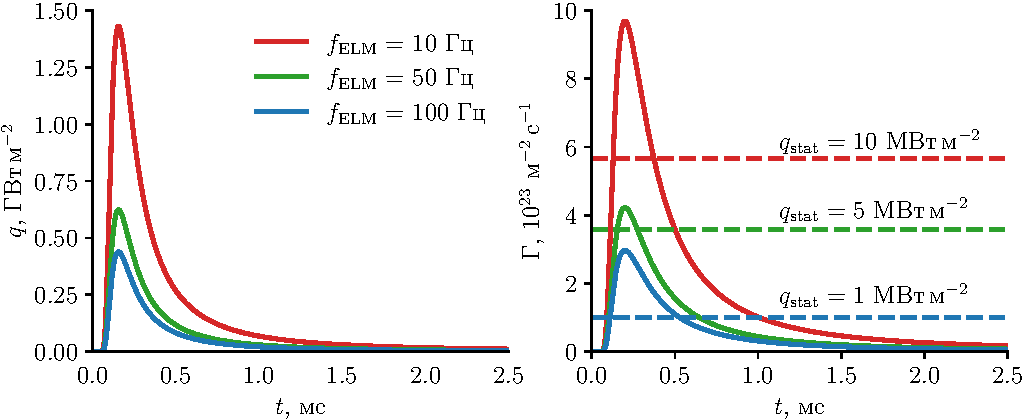
\includegraphics[scale=1]{ELM_fluxes.pdf}
	}
	\caption{Временные зависимости плотности потоков тепла (слева) и частиц (справа) во время ELM-событий при различных частотах повторения. Пунктирные линии соответствуют плотности потока частиц при стационарном облучении}\label{fig:ch3/ELM_fluxes}
\end{figure}

Исключение сделано в подразделе~\ref{subsec:ch3/sec2/subsec5}, где анализируется влияние отношения потока частиц к их энергии во время ELM-событий. Для этой части работы плотность потока частиц во время ELM масштабируется в $\beta$ раз, а энергия ионов "--- в $1/\beta$ раз, сохраняя плотность тепловой мощности. Таким образом, отношение плотности потока частиц к энергии увеличивается в $\beta^2$ раз. Параметры имплантации и отражения были рассчитаны для каждого случая и представлены в таблице~\cref{tab:flux_var_params}.
\begin{table}[ht]
	\caption{Параметры профиля внедренных частиц и коэффициент отражения ионов дейтерия при различных значениях энергии, соответствующих ELM-событиям} \label{tab:flux_var_params}
	\renewcommand{\arraystretch}{1.2}%% Увеличение расстояния между рядами, для улучшения восприятия.
	\begin{tabularx}{\linewidth}{>{\centering\arraybackslash}X>{\centering\arraybackslash}X>{\centering\arraybackslash}X>{\centering\arraybackslash}X>{\centering\arraybackslash}X>{\centering\arraybackslash}X}
		\toprule
		$\beta$ & $E$, \si{\electronvolt} & $r_{\mathrm{ELM}}$ & $r_{\mathrm{ELM}}^{E}$ & $X_{\mathrm{ELM}}$, \si{\nano\meter} & $\sigma_{\mathrm{ELM}}$, \si{\nano\meter} \\
		\hline
		\hline
		1,00    & 9400                    & 0,298              & 0,139                  & 73,4                                 & 38,2                                      \\
		1,33    & 7050                    & 0,334              & 0,164                  & 58,8                                 & 31,0                                      \\
		2,00    & 4700                    & 0,382              & 0,200                  & 43,4                                 & 23,2                                      \\
		2,50    & 3760                    & 0,407              & 0,218                  & 36,9                                 & 19,8                                      \\
		5,00    & 1800                    & 0,474              & 0,273                  & 22,7                                 & 12,3                                      \\
		10,00   & 940                     & 0,529              & 0,322                  & 14,4                                 & 7,8                                       \\
		\bottomrule
	\end{tabularx}
\end{table}

\subsection{Эволюция температуры}\label{subsec:ch3/sec2/subsec3}
Динамика температуры поверхности при $q_{\mathrm{stat}}=\SI{10}{\mega\watt\per\meter\squared}$ показана на рисунках~\cref{fig:ch3/ELM_T_a, fig:ch3/ELM_T_b} для нескольких частот ELM-событий. Временные зависимости быстро достигают квазиплато за время $\approx\SI{3}{\second}$, что намного короче ожидаемой продолжительности разряда ($\sim\SI{100}{\second}$) в ИТЭР. Квазиплато характеризуется индуцированными ELM-событиями колебаниями температуры, которая не превышает точку плавления вольфрама. В рамках описанной модели переходные нагрузки с более низкими частотами соответствуют более высоким колебаниям температуры (см. рисунок~\cref{fig:ch3/ELM_T_b}), но усредненная по длительности ELM-события температура поверхности растет противоположным образом, что показано пунктирными линиями.

\begin{figure}[ht]
	\centerfloat{
		\hfill
		\subcaptionbox[List-of-Figures entry]{\label{fig:ch3/ELM_T_a}}{%
			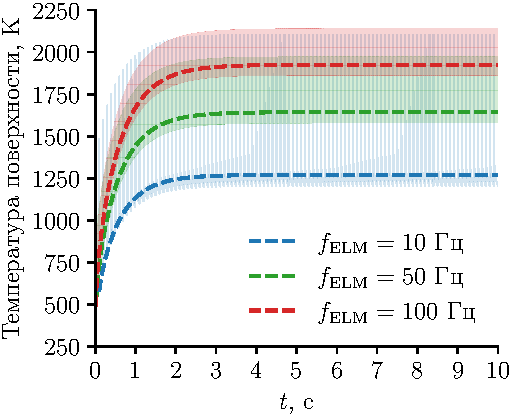
\includegraphics[scale=1]{T_surf.pdf}}
		\hfill
		\subcaptionbox{\label{fig:ch3/ELM_T_b}}{%
			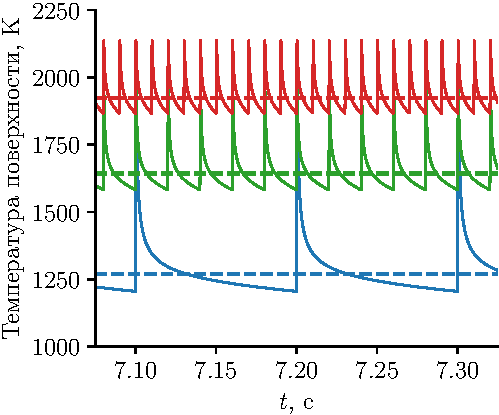
\includegraphics[scale=1]{T_surf_cut.pdf}} \\
		\subcaptionbox{\label{fig:ch3/ELM_T_c}}{%
			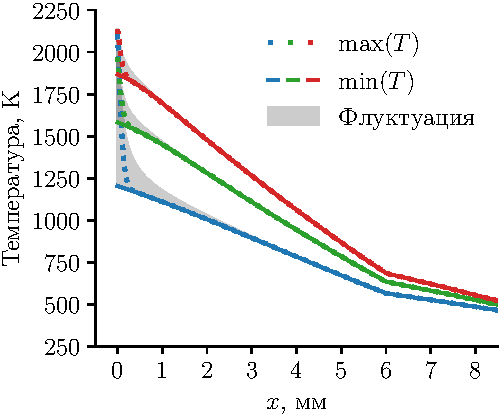
\includegraphics[scale=1]{T_profile.pdf}}
	}
	\caption{(а) Временная эволюция температуры передней поверхности при комбинированном нагреве с $q_{\mathrm{stat}}=\SI{10}{\mega\watt\per\meter\squared}$ и различных частотах ELM-событий. Пунктирные линии показывают зависимости, усредненные по длительности ELM-событий. Затененные области представляют собой отдельные колебания температуры, явно показанные на рисунке (б). (в) Область изменения температуры вдоль композитной геометрии за один период колебаний из рисунка (б). Сплошные и пунктирные линии показывают распределения температуры по глубине при достижении максимального и минимального значений на поверхности}
\end{figure}

После наступления квазиплато пространственное изменение температуры локализовано в объеме вольфрама. Это можно заметить на рисунке~\cref{fig:ch3/ELM_T_c}, где затененные области определяют рассчитанные изменения температуры за один период. Более глубокая часть композитной геометрии остается в пределах квазистационарного режима, что согласуется с более ранним анализом~\cite{Marenkov2012a}. Более того, размер возмущенной зоны уменьшается с частотой ELM-событий. Данное наблюдение позволяет ограничить рассмотрение только областью вольфрама. Для сохранения временной эволюции температуры неизменной тепловой поток на границе раздела W-Cu был параметризован:
\begin{subequations}
	\label{eq:ch3/heat_WCu}
	\begin{align}
		q^*_{\mathrm{loss}}         & =\overline{q}_{\mathrm{tot}}\,\left(a+b(T-T_0)-c\,\exp\left( -\dfrac{T-T_0}{d}\right)\right),\label{eq:ch3/heat_WCu1} \\
		\overline{q}_{\mathrm{tot}} & =q_{\mathrm{stat}}+f_{\mathrm{ELM}}\int\limits_{\tau_{\mathrm{ELM}}}q_{\mathrm{ELM}}dt. \label{eq:ch3/heat_WCu2}
	\end{align}
\end{subequations}
Второй член в уравнении~\cref{eq:ch3/heat_WCu2} представляет собой среднюю по длительности ELM-события плотность мощности и, принимая во внимание уравнении~\cref{eq:ch3/norm_elm_hf}, просто равен $\overline{q}_{\mathrm{ELM}}=f_{\mathrm{ELM}}\varepsilon_{\parallel}\sin(\alpha)$. Параметры, определяющие выражения~\cref{eq:ch3/heat_WCu} приведены в таблице~\cref{tab:fit_params}. Эти выражения затем использовались в граничном условии для уравнения теплопроводности.

\subsection{Влияние параметров импульсно-периодических нагрузок}\label{subsec:ch3/sec2/subsec5}

Накопление дейтерия при комбинированном (стационарном и импульсно-периодическом) облучении было проанализировано в зависимости от частоты ELM-событий и параметров стационарного (фонового) облучения при $E_{\mathrm{dt}}=\SI{1.5}{\electronvolt}$; $n_{t}=\SI{e-2}{\text{ат.}\percent}$; $E_{\mathrm{ELM}}=2\, T_{\mathrm{e,ped}}$. Сплошными линиями на рисунке~\cref{fig:ch3/ELMs_frequency} показаны временные зависимости температуры поверхности и интегрального содержания дейтерия ($\int \left(c_{\mathrm{m}}+c_{\mathrm{tr}}\right)dx$) для \SI{1000}{\second} непрерывного облучения в трех сценариях моделирования. Для наглядности представлены только усредненные по длительности ELM-события зависимости. Пунктирные линии соответствуют случаю без ELM-событий.
\begin{figure}[ht]
	\centerfloat{
		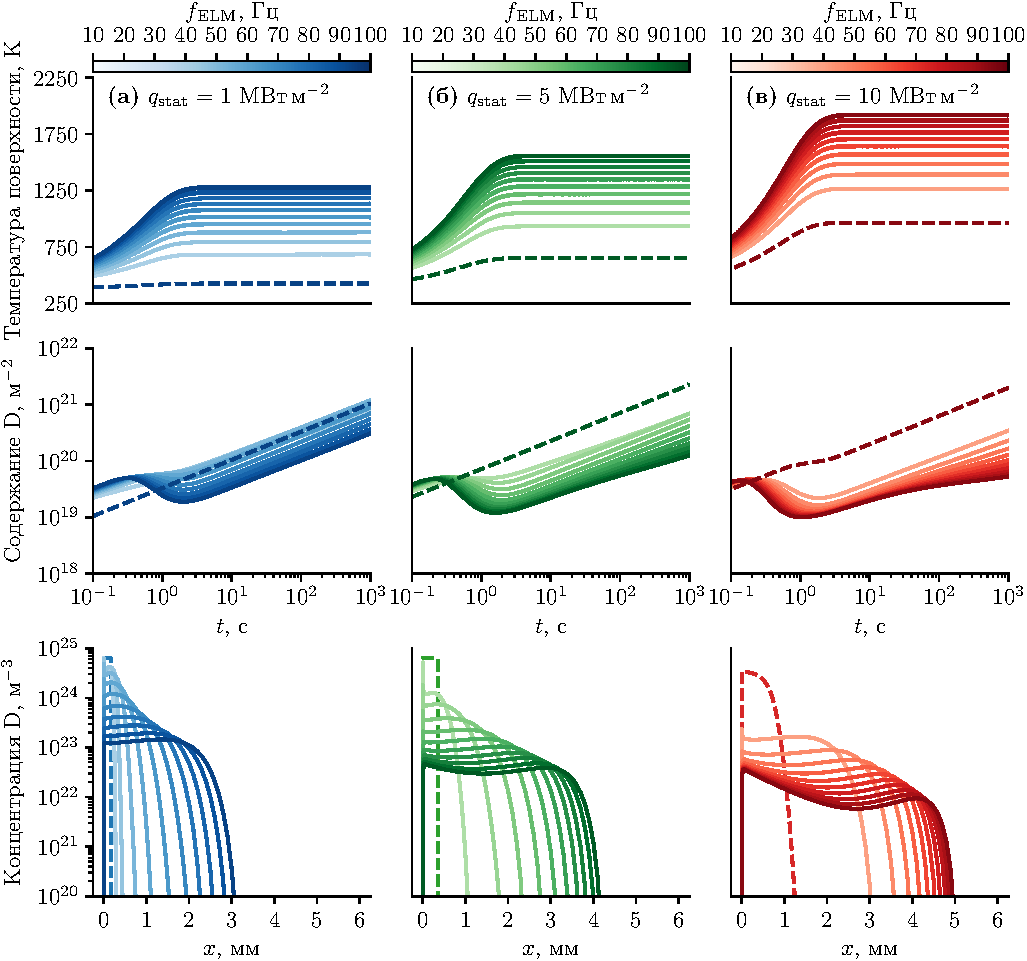
\includegraphics[scale=1]{ELMs_frequency.pdf}
	}
	\caption{Временные зависимости усредненной по длительности ELM-событий температуры поверхности (верхний ряд) и содержания дейтерия (средний ряд) при различных стационарных нагрузках. Пунктирные линии показывают соответствующие зависимости в случае без ELM-событий. Нижний ряд демонстрирует распределения концентрации дейтерия по глубине на последнем временном шаге}\label{fig:ch3/ELMs_frequency}
\end{figure}
На ранних стадиях ($t<1$ с) комбинированное облучение приводит к увеличению интегральной концентрации дейтерия, удерживаемого в вольфраме. Данный рост можно легко понять из оценки максимальной концентрации подвижных атомов при имплантации в приближении мгновенной десорбции:
\begin{equation}
	\label{eq:ch3/max_c}
	c_{\mathrm{m}}^{\max}\propto \frac{\Gamma^{\mathrm{impl}} \, X}{D(T)}.
\end{equation}
При низких температурах дополнительный поток атомов во время ELM-событий повышает значение $c_{\mathrm{m}}^{\max}$. Поскольку нагрузки идентичны во всех сценариях, увеличение более очевидно при $q_{\mathrm{stat}}=\SI{1}{\mega\watt\per\meter\squared}$ (см. столбец (a) на рисунке~\cref{fig:ch3/ELMs_frequency}), где фоновые нагрузки самые низкие. В этом случае повышенное накопление наблюдается и для более высоких доз облучения при низких частотах ELM-событий, когда среднее повышение температуры и, соответственно, скорость десорбции не высоки. Можно предположить, что эти наблюдения коррелируют с экспериментальными результатами, полученными на КСПУ-Т~\cite{Ogorodnikova,Poskakalov2020}, где существенный захват дейтерия наблюдался при небольшом количестве плазменных выстрелов с большим временем между импульсами.

С другой стороны, в большинстве случаев наблюдается спад в содержании дейтерия после наступления квазиплато температуры поверхности ($t>1$ с). Уменьшение содержания увеличивается с частотой ELM-событий и величиной фоновой нагрузки. Дополнительный нагрев во время ELM повышает среднюю температуру минимум на $\sim\SI{260}{\kelvin}$ (\SI{10}{\hertz}, \SI{1}{\mega\watt\per\meter\squared}) и максимум на $\sim\SI{1000}{\kelvin}$ (\SI{100}{\hertz}, \SI{10}{\mega\watt\per\meter\squared}). Этот рост температуры вызван приходом высокоэнергетичных ($E\sim T_{\mathrm{e,ped}}$) частиц во время ELM-событий с плотностью потока близкой к случаю стационарных нагрузок. Таким образом, результирующий эффект заключается в снижении интегрального содержания дейтерия, что согласуется с более ранними исследованиями~\cite{Hu2015}. Нагрев до более высоких температур также инициирует интенсивную миграцию дейтерия в объем. Для иллюстрации в нижнем ряду рисунка~\cref{fig:ch3/ELMs_frequency} представлены распределения глубины концентрации дейтерия при $t=\SI{1000}{\second}$. Из рисунка видно, что дейтерий проникает гораздо глубже в объем при комбинированном облучении. В стационарных условиях аналогичные пространственные масштабы миграции на уровне миллиметров могут быть достигнуты при более длительном облучении~\cite{Hodille2021}.

Интерес также представляет динамика изменения коэффициента рециклинга (\( R \)) во время ELM-событий:
\begin{equation}
	R = \frac{J_\mathrm{des}}{\Gamma^{\mathrm{impl}}_\mathrm{stat}+\Gamma^{\mathrm{impl}}_\mathrm{ELM}},
\end{equation}
где поток десорбированных частиц определяется на основе диффузионного потока вблизи облучаемой поверхности. Из результатов расчетов следует, что коэффициент рециклинга быстро достигает квазиплато вблизи значения равного единице. На рисунке~\cref{fig:ch3/R_freq} приведены временные зависимости коэффициента рециклинга на узком временном промежутке после первой секунды облучения.   
\begin{figure}[ht]
	\centerfloat{
		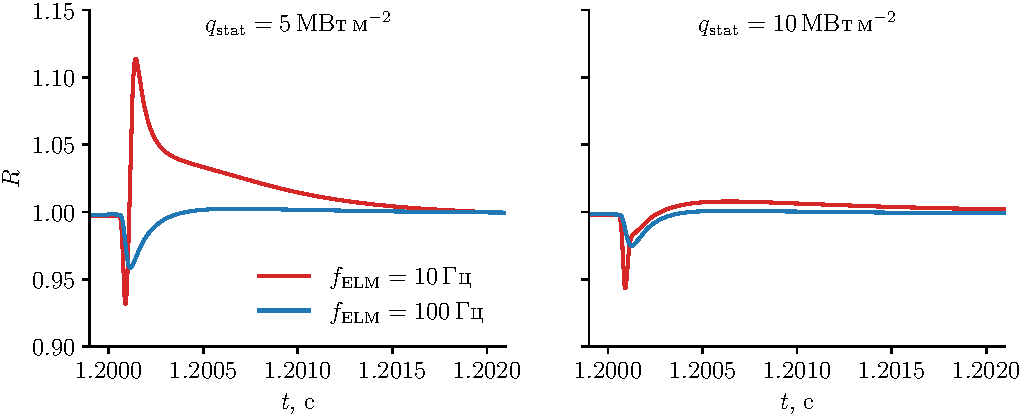
\includegraphics[scale=1]{R_freq.pdf}
	}
	\caption{Временная эволюция коэффициента рециклинга в двух сценариях облучения при разных частотах ELM-событий}\label{fig:ch3/R_freq}
\end{figure}

Начало ELM-события во всех случаях сопровождается резким спадом коэффициента рециклинга за счет появления дополнительного источника внедряемых атомов. За счет повышения температуры и градиента концентрации вблизи поверхности увеличивается обратный поток газовыделения, который приводит либо к превышению значения \(R=1\) (при низких частотах ELM-событий), либо к приближению к равновесной ситуации (при высоких частотах ELM-событий). В случае низких частот дальнейшее достижение равновесия происходит на временном масштабе, соизмеримом с длительностью потоков тепла и частиц во время ELM-событий, но меньшем периода их повторения. Полученные результаты согласуются с ранними работами~\cite{Schmid2016,Smirnov2024}, где наблюдались аналогичные закономерности. Такая динамика позволяет предположить, что в случае <<холодных>> сценариев облучения, когда ОПЭ подвергается воздействию низких потоков тепла и частиц (например, области, удаленные от точки удара), крупные ELM-события могут приводить к отклонению значения коэффициента рециклинга от близкого к единице, которое не будет успевать достигнуть равновесного значения за время восстановления пьедестала и повторного выброса плазмы.  

Как продемонстрировано, FSM модель позволяет анализировать качественные закономерности накопления изотопов водорода во время ELM-событий. Однако поток ионов, приходящих на поверхность во время ELM-событий, может изменяться вблизи мишени из-за вторичных эффектов, не охватываемых уравнениями~\cref{eq:ch3/elm_fluxes}. Эти выражения были выведены в предположении бесстолкновительного переноса филамента из области пьедестала к идеально поглощающим границам в отсутствие фоновой плазмы. Поэтому некоторые процессы, например, взаимодействие быстрых ионов с частицами вблизи мишени может приводить к изменению параметров облучения.

В работе~\cite{Guillemaut2018} было предложено, что процесс резонансной перезарядки (CX) может приводить к увеличению потока частиц/тепла на поверхность (см. схематическую диаграмму на рисунке~\cref{fig:ch3/redeposition}) при взаимодействии быстрых частиц (быстрый ион "--- быстрый отраженный атом). Аналогичным образом быстрые ионы могут взаимодействовать с медленными атомами, образованными из-за отражений или диссоциации десорбированных молекул, например, электронным ударом (EI). В ходе CX-процесса быстрые частицы могут передавать часть своей энергии более медленным, уменьшая среднюю энергию частиц, приходящих на поверхность. Наконец, медленные атомы могут становиться ионами посредством прямого электронного удара. 
\begin{figure}[ht]
	\centerfloat{
		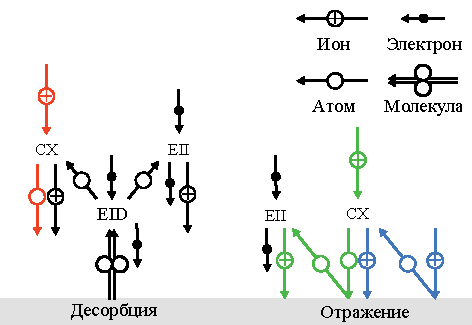
\includegraphics[scale=1.5]{Flux_diagram_simple_rus.pdf}
	}
	\caption{Схематическое представление возможных процессов вблизи поверхности мишени, приводящих к увеличению потока частиц во время ELM-событий: CX "--- резонансная перезарядка, EII "--- ионизация электронным ударом, EID "--- диссоциация электронным ударом}\label{fig:ch3/redeposition}
\end{figure}

Вероятность протекания каждого процесса требует отдельной оценки для конкретных параметров плазмы и приходящих ионов в ходе ELM-событий. Тем не менее в рамках данной работы проведена оценка влияния перераспределения потока и энергии частиц. Для анализа полагается, что процессы вблизи мишени приводят к изменению потока частиц в \( \beta \) раз с одновременным пропорциональным уменьшением их энергии, поэтому отношение плотности потока частиц к энергии увеличивается на $\beta^2$ при сохранении потока тепла на поверхность. Параметр $\beta$ варьировался в диапазоне от 1 до 10 при остальных параметрах, что и в предыдущих расчетах. 

На рисунке~\cref{fig:ch3/beta_var} показаны рассчитанные значения содержания дейтерия в вольфраме после \SI{1000}{\second} комбинированного облучения при разных частотах ELM-событий. 
\begin{figure}[bt]
	\centerfloat{
		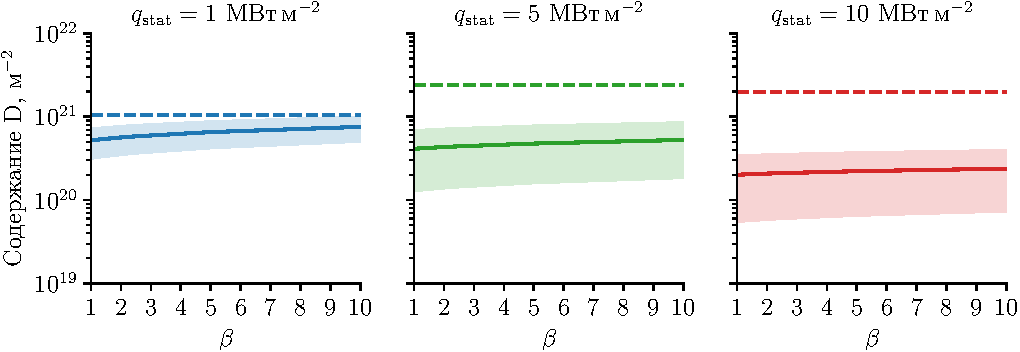
\includegraphics[scale=1]{beta_var.pdf}
	}
	\caption{Зависимости интегрального содержания дейтерия в вольфраме после \SI{1000}{\second} облучения при различных значениях отношения плотности потока частиц, приходящих во время ELM-событий, к их энергии. Сплошные линии обозначают средние значения содержания при комбинированном облучении с различными частотами ELM-событий. Верхние границы заштрихованных областей соответствуют \(f_\mathrm{ELM} = \SI{10}{\hertz}\), нижние "--- \(f_\mathrm{ELM} = \SI{100}{\hertz}\). Пунктирные линии показывают зависимости, полученные только при стационарном облучении}\label{fig:ch3/beta_var}
\end{figure}
Увеличение $\beta$ более явно приводит к росту содержания при меньших стационарных нагрузках. Это наблюдается как при фиксированной частоте, так и при фиксированной величине стационарной нагрузки. Можно также заметить, что в случае прихода низкоэнергетичных частиц с большой плотностью потока содержание дейтерия может достигнуть уровня, соответствующего только стационарному облучению. Качественно, повышение скорости накопления дейтерия можно понять из уравнения~\cref{eq:ch3/max_c}: увеличение $\beta$ незначительно повышает произведение $\beta\Gamma (1-r) X(E/\beta)$ ввиду снижения характерной глубины внедрения и увеличения коэффициента отражения. 

\subsection{Влияние параметров центров захвата и скорости рекомбинации на поверхности}

Параметры дефектов определяют вероятности захвата и освобождения атомов дейтерия. Очевидно, что вероятность выхода из дефекта тем больше, чем меньше энергетический барьер для этого. Также ожидается, что материалы с высокой концентрацией дефектов будут характеризоваться большей способностью накапливать дейтерий, чем материалы с идеальной кристаллической структурой. Упомянутые эффекты проиллюстрированы на рисунке~\cref{fig:ch3/eta_Edt_var}, где показаны результаты моделирования при различных значениях концентрации центров захвата и энергетического барьера выхода из них. Во всех сценариях итоговое содержание дейтерия увеличивается с концентрацией дефектов (см. верхний ряд графиков), что согласуется с известными экспериментальными закономерностями. Однако, все еще наблюдается снижение интегрального накопления дейтерия при комбинированном облучении. Причем, разница между значениями растет с концентрацией дефектов.
\begin{figure}[ht]
	\centerfloat{
		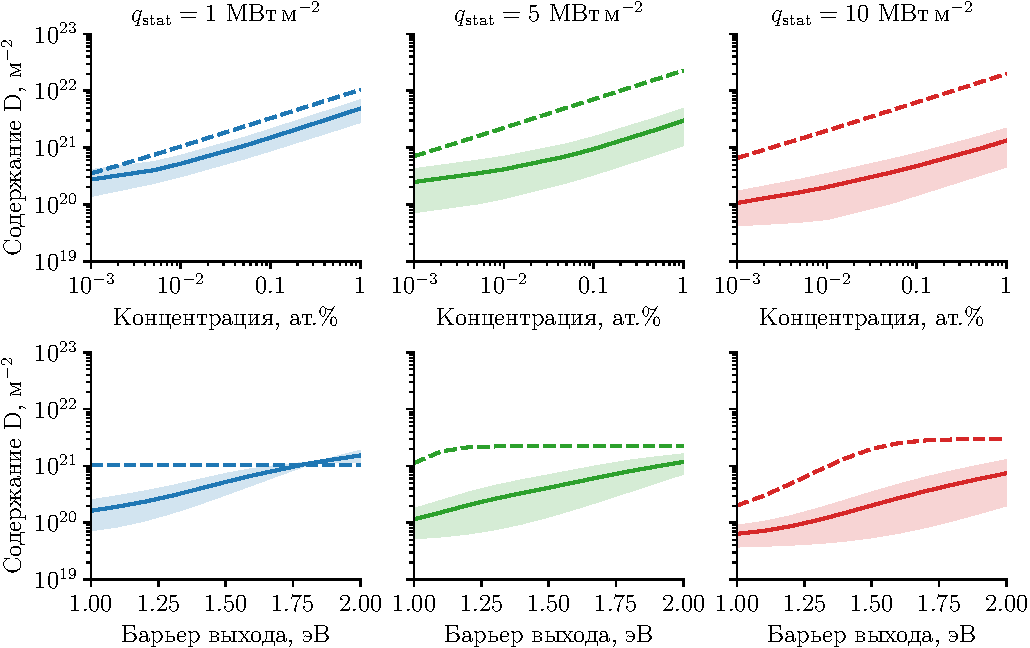
\includegraphics[scale=1]{eta_Edt_var.pdf}
	}
	\caption{Зависимости интегрального содержания дейтерия в вольфраме после \SI{1000}{\second} облучения при различных значениях концентрации дефектов (верхний ряд) и барьера выхода из них (нижний ряд). Сплошные линии обозначают средние значения содержания при комбинированном облучении с различными частотами ELM-событий. Верхние границы заштрихованных областей соответствуют \(f_\mathrm{ELM} = \SI{10}{\hertz}\), нижние "--- \(f_\mathrm{ELM} = \SI{100}{\hertz}\). Пунктирные линии показывают зависимости, полученные только при стационарном облучении}\label{fig:ch3/eta_Edt_var}
\end{figure}

Влияние барьера выхода из дефектов на накопление показано в нижнем ряду рисунка~\cref{fig:ch3/eta_Edt_var}. В низкотемпературных режимах (только стационарное облучение при $q_{\mathrm{stat}}=\SI{1}{\mega\watt\per\meter\squared}$) нет зависимости от величины барьера выхода с точки зрения удержания, поскольку все имплантированные атомы становятся неподвижными. В высокотемпературных режимах содержание увеличивается с барьером освобождения, так как большая часть атомов подвижных может оставаться в захваченном состоянии. Поэтому разница между стационарным и комбинированным воздействием нивелируется для случая дефектов с большим барьером освобождения. Значения интегрального содержания могут быть соизмеримы при низких стационарных нагрузках.

Сделанные выводы согласуются с известными закономерностям удержания топлива в ОПЭ, но более важным является увеличение удержания с концентрацией центров захвата и барьером освобождения из них. Это предполагает, что образование высокоэнергетичных центров захвата в объеме материала во время работы установки типа ИТЭР (например, из-за нейтронного облучения) может создать условия для повышения скорости накопления изотопов водорода. Это повышение может компенсировать снижение, вызванное дополнительным тепловым потоком, приносимым высокоэнергетическими частицами в течение ELM-событий.

До сих пор представленные расчеты проводились в приближении мгновенной рекомбинации и десорбции на передней поверхности вольфрама. В зависимости от состояния поверхности скорость десорбции может меняться, влияя на динамику удержания изотопов водорода. Для иллюстрации роли этого процесса на рисунке~\cref{fig:ch3/rec_var} показаны значения содержания дейтерия при различной скорости рекомбинации, варьируемой за счет изменения барьера хемосорбции на поверхности ($E_{\mathrm{c}}$). Для полноты также приведены два частных случая в приближениях мгновенной рекомбинации ($\infty$) и <<чистой>> поверхности ($E_{\mathrm{c}}=0$).

\begin{figure}[ht]
	\centerfloat{
		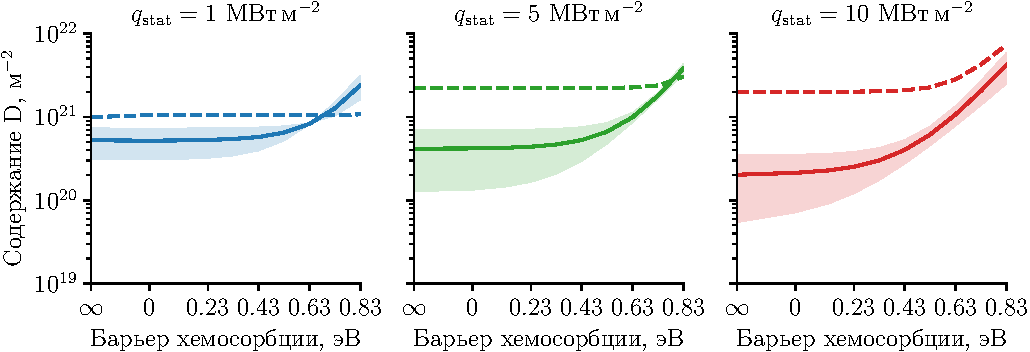
\includegraphics[scale=1]{rec_var.pdf}
	}
	\caption{Зависимости интегрального содержания дейтерия в вольфраме после \SI{1000}{\second} облучения при различных значениях скорости рекомбинации на поверхности. Сплошные линии обозначают средние значения содержания при комбинированном облучении с различными частотами ELM-событий. Верхние границы заштрихованных областей соответствуют \(f_\mathrm{ELM} = \SI{10}{\hertz}\), нижние "--- \(f_\mathrm{ELM} = \SI{100}{\hertz}\). Пунктирные линии показывают зависимости, полученные только при стационарном облучении}\label{fig:ch3/rec_var}
\end{figure}

Согласно данным, приближение мгновенной рекомбинации воспроизводит результаты, полученные при низких значениях барьера хемосорбции. Увеличение барьера хемосорбции снижает скорость рекомбинации на поверхности, что приводит к росту скорости накопления дейтерия. Это увеличение более явно наблюдается в случае комбинированного воздействия, поскольку используемый коэффициент рекомбинации Пика и Сонненберга уменьшается с температурой. Анализируя данные для наибольшего значения барьера хемосорбции, можно заметить, что результаты при комбинированном воздействии близки к полученным без учета ELM-событий. Это позволяет предположить возможное повышение скорости накопления дейтерия в случае образования на поверхности потенциального барьера, например, из-за примесных атомов.

\subsection{Эффективность обезгаживания}

Все приведенные результаты указывают на снижение скорости накопления при наступлении ELM-событий. В то же время нагрев до более высоких температур относительно базовых нагрузок приводит к миграции дейтерия в объем, где он накапливается в дефектах. Помимо того, что ускоренная диффузия может влиять на время проникновения в систему охлаждения, она также может усложнять процесс удаления трития. В ИТЭР в качестве базовых механизмов для этого рассматриваются изотопный обмен и прогрев ОПЭ, причем второй подход предполагается использовать для обезгаживания толстых поверхностных слоев (в том числе и соосажденных слоев). Во время длительных этапов обслуживания планируется осуществлять нагрев ОПЭ за счет пропускания горячей воды под давлением через систему охлаждения моноблоков. При таком подходе возможно достижение температуры ОПЭ в \SI{513}{\kelvin}~\cite{Pitts2025}.

Для оценки влияния появления ELM-событий на эффективность последующего обезгаживания ОПЭ была проведена дополнительная серия расчетов. Рассматривалось три этапа: облучение длительностью \SI{100}{\second}; простой и охлаждение материала длительностью \SI{1}{\hour}; обезгаживание материала при постоянной температуре \SI{513}{\kelvin} длительностью \SI{25}{\day}. Расчеты были проведены с одним типом центров захвата с концентрацией \SI{e-2}{\text{ат.}\percent} и барьером освобождения \SI{1}{\electronvolt}. 

Пример полученных временных зависимостей температуры поверхности и содержания дейтерия в вольфраме приведен на рисунке~\cref{fig:ch3/baking_single} для двух случаев облучения: при учете влияния ELM-событий и без.
\begin{figure}[ht]
	\centerfloat{
		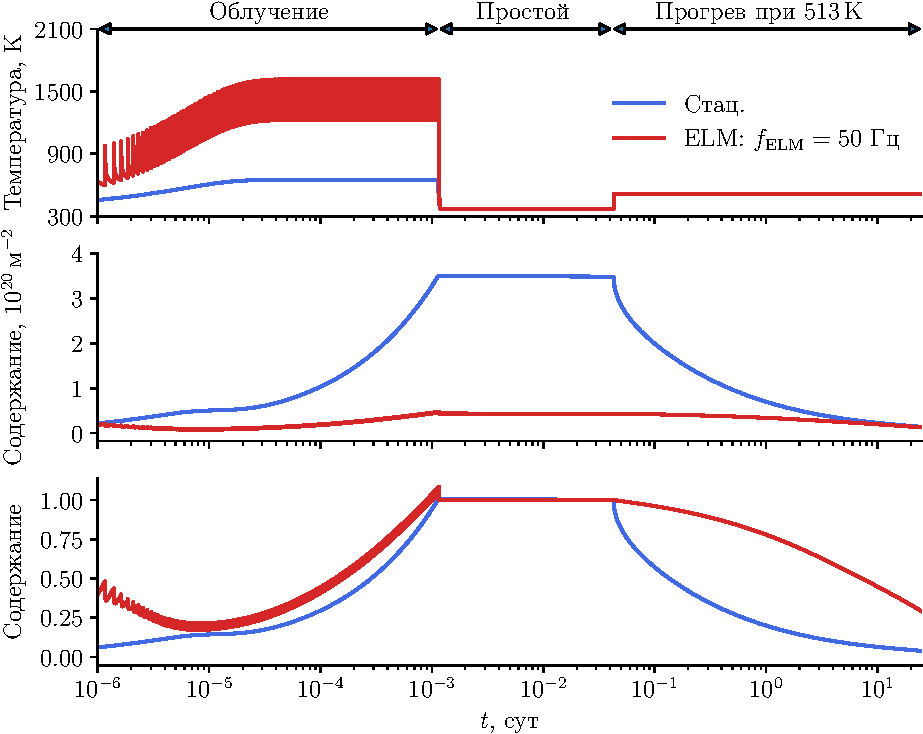
\includegraphics[scale=1]{baking_single.pdf}
	}
	\caption{Временные зависимости температуры поверхности (вверху), содержания дейтерия (по середине) и содержания дейтерия, нормированного на значение в начале процедуры обезгаживания для двух случаев облучения при \(q_\mathrm{stat}= \SI{5}{\mega\watt\per\meter\squared}\)}\label{fig:ch3/baking_single}
\end{figure}
В случае только стационарного облучения содержание существенно превышает достигаемое значение при ELM-событиях. После начала процедуры обезгаживания в обоих случаях наблюдается уменьшение количества захваченных атомов, однако зависимость в случае ELM-событий спадает более плавно, что напрямую связано с пространственным распределением захваченного дейтерия на момент начала процедуры.

Расчетная эффективность обезгаживания (интегральное число десорбированных частиц отнесенное к их начальному количеству) для всех сценариев облучения приведена на рисунке~\cref{fig:ch3/baking_efficiency}.
\begin{figure}[ht]
	\centerfloat{
		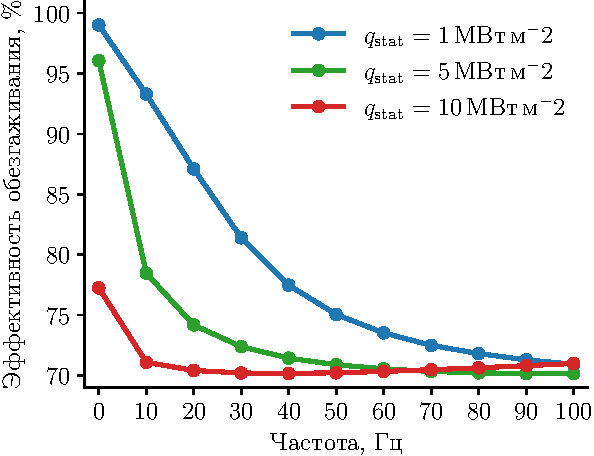
\includegraphics[scale=1]{baking_efficiency.pdf}
	}
	\caption{Зависимость эффективности обезгаживания от частоты ELM-событий в трех модельных сценариях облучения. Значения при нулевой частоте соответствуют случаю облучения только стационарными потоками тепла и частиц}\label{fig:ch3/baking_efficiency}
\end{figure}
Из рисунка видно, что наибольшая эффективность достигается в случае только стационарного облучения. С увеличением фоновой нагрузки и частоты ELM-событий эффективность уменьшается, что вызвано проникновением дейтерия на большую глубину при нагреве материала до более высоких температур. Можно также заметить, что при высоких частотах эффективность обезгаживания в самом <<горячем>> сценарии немного увеличивается. Это вызвано достижением атомами дейтерия правой границы расчетной области за рассмотренное время процедуры. Таким образом, проведенное моделирование явно демонстрирует, что протекание переходных процессов может влиять как на скорость накопления дейтерия во время плазменных разрядов, так и на эволюцию его содержания в ОПЭ во время иных этапов эксплуатации установки. 

\section{Аналитический анализ}\label{sec:ch3/sec3}

В предыдущем разделе были представлены результаты моделирования, ограниченного случаем \SI{1000}{\second} непрерывного облучения во время ELM-событий. Ввиду необходимости использования малого временного шага интегрирования расчеты такого типа оказываются более времязатратными, чем в случае моделирования накопления изотопов водорода при стационарном облучении. Время расчета на одном ядре процессора Intel Xeon Gold 6240 достигало \SI{72}{\hour} в случае непрерывного облучения при частоте ELM-событий равной \SI{100}{\hertz}. Данное время является приемлемым, но указывает на то, что решение аналогичной задачи в трехмерной геометрии на временных масштабах, соизмеримых со сроком службы установки (\( \sim \SI{e6}{\second}\)), потребует гораздо больших временных и вычислительных ресурсов. В аналогичном исследовании~\cite{Dasgupta2023} рассматривался захват дейтерия под действием импульсно-периодических тепловых нагрузок при стационарном потоке частиц и без учета влияния дефектов. В работе было предложено использовать осредненный по длительности ELM-события тепловой поток для упрощения моделирования и снижения вычислительных затрат. В этом разделе проведен анализ применимости подхода к решению полной задачи транспорта дейтерия в вольфраме.

\subsection{Квазистационарное приближение}
Переход к осредненным величинам (так называемое осреднение по Рейнольдсу) подразумевает разделение периодических потоков тепла и частиц на медленно меняющиеся и флуктуирующие части~\cite{Marenkov2012a}:
\begin{subequations}
	\label{eq:ch3/periodic_funcs}
	\begin{align}
		q_{\mathrm{ELM}}(t)&=\overline{q}_{\mathrm{ELM}} + \widetilde{q}_{\mathrm{ELM}}(t),\label{eq:decomp_heat}\\
		\Gamma_{\mathrm{ELM}}(t)&=\overline{\Gamma}_{\mathrm{ELM}} + \widetilde{\Gamma}_{\mathrm{ELM}}(t),
	\end{align}
\end{subequations}
где $\overline{q}_{\mathrm{ELM}}$ ($\overline{\Gamma}_{\mathrm{ELM}}$) "--- средний по времени поток тепла (частиц), приходящий за период ELM-события. Средние значения легко получить путем интегрирования выражений~\cref{eq:ch3/elm_fluxes}:
\begin{subequations}
	\label{eq:ch3/av_funcs}
	\begin{align}
		\overline{q}_{\mathrm{ELM}}&=f_{\mathrm{ELM}}\varepsilon_\parallel\sin(\alpha)\label{eq:av_heat},\\
		\overline{\Gamma}_{\mathrm{ELM}}& =\frac{\sqrt{\pi}}{2} \Gamma_{0,\mathrm{ELM}}\,\psi\,\mathrm{erfc}\left(\psi\right),\label{eq:av_flux}
	\end{align}
\end{subequations}
где $\psi=\tau f_{\mathrm{ELM}}$, $\mathrm{erfc(x)}$ "--- дополнительная функция ошибок.

Подстановка разложенного теплового потока в уравнение теплопроводности позволяет отдельно проанализировать поле средней температуры. Несмотря на то, что тепловые свойства материала зависят от температуры нелинейно, вклад их изменения в эволюцию средней температуры материала будет небольшим. Индуцированное повышение температуры из-за поверхностного теплового импульса пропорционально $1/\sqrt{\kappa C \rho}$, которое медленно меняется с температурой. С другой стороны, полное аналитическое рассмотрение реакционно-диффузионной задачи гораздо сложнее, учитывая экспоненциальную зависимость констант скорости процессов от температуры.

Основной интерес в вопросе длительного накопления изотопов водорода в ОПЭ представляет среднее значение содержания, которое будет сохраняться по окончании плазменного разряда. Провести аналитический анализ можно в приближении малых ELM-вспышек~\cite{Marenkov2012a}, когда амплитуды флуктуирующих компонент потоков малы по сравнению со средними. В данном приближении эволюция концентрации атомов будет определяться средними компонентами вплоть до достижения квазистационарного режима. В случае больших ELM-вспышек, члены, связанные с флуктуациями, будут влиять на изменение средних компонент. Чтобы различить эти два случая, можно сравнить средние и флуктуирующие компоненты температуры и объемного источника атомов в задаче транспорта дейтерия.

Пренебрегая охлаждением за счет излучения, подстановка компонент потока тепла с последующим осреднением уравнения теплопроводности по длительности ELM-события позволяет легко получить квазистационарное распределение температуры:
\begin{equation}
	\label{eq:ch3/temp_av}
	\overline{T}(x)=T_\mathrm{r}+\overline{q}_{\mathrm{tot}}\,\int\limits_x^L\frac{dx}{\kappa(\overline{T})},
\end{equation}
где, $T_\mathrm{r}$ "--- равновесная температура на задней границе материала, которая находится из баланса теплового потока: $\overline{q}_{\mathrm{tot}}=q_{\mathrm{loss}}^*(T_\mathrm{r})$ (см. уравнение~\cref{eq:ch3/heat_WCu}). Максимальное колебание температуры из-за потока тепла на границе можно оценить как:
\begin{equation}
	\label{eq:ch3/temp_fluct}
	\widetilde{T}^{\max} \propto \widetilde{q}_{\mathrm{ELM}}^{\max} \sqrt{\frac{\tau}{\kappa C \rho}}.
\end{equation} 

Вычислив значение среднего теплового потока, можно заметить, что $\widetilde{q}_{\mathrm{ELM}}^{\max} \approx q_{\mathrm{ELM}}^{\max}$. Тепловой поток во время ELM-события достигает максимального значения $q_{\mathrm{ELM}}^{\max}\approx 0.84 \, q_{0,\mathrm{ELM}}$ при $\tau/t\approx 1.27$. Индуцированное колебание температуры можно считать малым, если $\widetilde{T}^{\max} \ll \overline{T}(x=0)$. Оценку можно получить, полагая, что свойства материала не зависят от температуры:
\begin{equation}
	\label{eq:heat_condition}
	q_{0,\mathrm{ELM}} \ll \overline{q}_{\mathrm{tot}}\,\frac{ L}{L_{\mathrm{heat}}}\,\left( 1+\frac{T_\mathrm{r}\kappa}{\overline{q}_{\mathrm{tot}}L}\right),
\end{equation}
где $L_{\mathrm{heat}}=\sqrt{\kappa\tau/C\rho}$ "--- характерная глубина распространения тепла за время длительности ELM-события. Для объемных источников атомов справедливо аналогичное соотношение: $\widetilde{S}^{\max}_{\mathrm{ELM}} \ll \overline{S}_{\mathrm{tot}}$, где $\overline{S}_{\mathrm{tot}}=S_{\mathrm{stat}}+\overline{S}_{\mathrm{ELM}}$. Аналогично предыдущему случаю, максимальная амплитуда флуктуации потока частиц из-за ELM-вспышки приблизительно равна: $\widetilde{\Gamma}_{\mathrm{ELM}}^{\max} \approx \Gamma_{\mathrm{ELM}}^{\max}$. Поток частиц достигает максимума при $t=\tau$ со значением $\Gamma_{0,\mathrm{ELM}}/\exp(1)$. Обобщая начальное соотношение и используя параметры пространственного распределения источников, можно прийти к следующему условию:
\begin{equation}
	\label{eq:flux_condition}
	\Gamma_{0,\mathrm{ELM}} \ll \Gamma_{\mathrm{stat}}\,\frac{\varphi_{\mathrm{stat}}(X_\mathrm{stat})(1-r_{\mathrm{stat}})}{\varphi_{\mathrm{ELM}}(X_\mathrm{ELM})(1-r_{\mathrm{ELM}})}.
\end{equation}
Оба соотношения наглядно демонстрируют требование малости амплитуд осциллирующих компонент потоков во время ELM-событий. Исходя из предыдущего раздела, такие условия могут быть достигнуты при высоких частотах ELM-событий. Стоит заметить, что соотношения не являются независимыми, поскольку поток тепла зависит от потока частиц.

Для демонстрации применимости подхода на рисунке~\cref{fig:ch3/Eqv_load} приведено сравнение временных зависимостей содержания дейтерия, полученных двумя способами: путем моделирования накопления под действием обеих компонент потоков и с помощью только средних потоков. В соответствии с приведенным выше анализом отклонение результатов, полученных со средними компонентами потоков, уменьшается при более высоких частотах ELM-событий и фоновых нагрузках. В случае $q_{\mathrm{stat}}=\SI{10}{\mega\watt\per\meter\squared}$ результаты хорошо согласуются во всем диапазоне ELM-частот. Использование средних компонент потоков существенно снижает время вычислений (с дней до минут), что может быть использовано при проведении комплексных оценок накопления изотопов водорода во всей первой стенке ИТЭР.

\begin{figure}[ht]
	\centerfloat{
		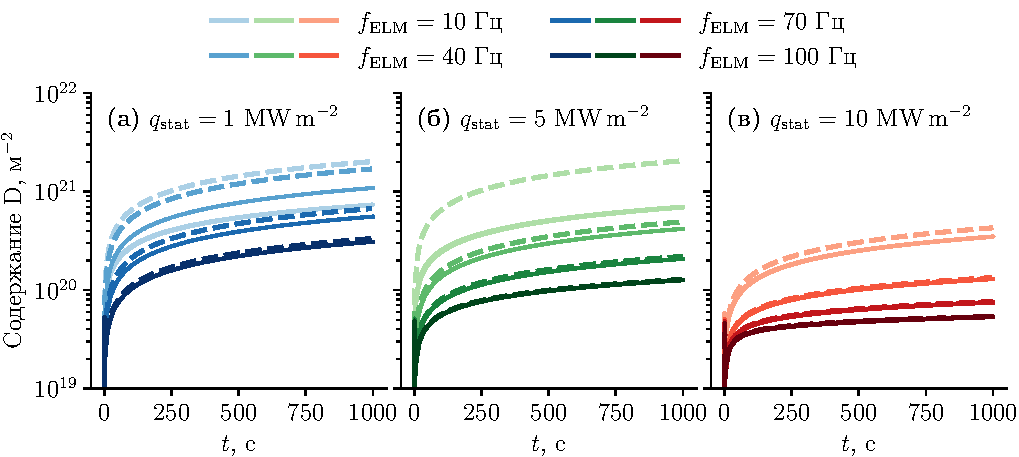
\includegraphics[scale=1]{Eqv_load.pdf}
	}
	\caption{Сравнение временных зависимостей содержания дейтерия, полученных при моделировании с учетом обеих компонент потоков тепла и частиц (сплошные линии) и с учетом только средних компонент (пунктирные линии)}\label{fig:ch3/Eqv_load}
\end{figure}

\subsection{Распределение концентрации дейтерия при насыщении}\label{sec:ch3/sec3/subsec2}
Использование средних компонент нагрузок позволяет получить аналитические выражения для распределения концентрации дейтерия при насыщении с учетом влияния градиента температуры, что является обобщением выражений, полученных ранее~\cite{Denis2022}. Рассмотрим стационарную форму задачи транспорта~\cref{eq:ch2/mobile_conc}, полагая что источники подвижных атомов являются точечными и каждый из них расположен на характерной глубине внедрения:
\begin{subequations}
	\label{eq:ch3/eq:solute_analytic}
	\begin{gather}
	\frac{\partial}{\partial x}\left(D(\overline{T})\left[\frac{\partial \overline{c}_{\mathrm{m}}}{\partial x} +H(\overline{T})\overline{c}_{\mathrm{m}}\right] \right)= - S_{\mathrm{stat}}^{\delta}-\overline{S}_{\mathrm{ELM}}^{\delta}, \label{eq:ch3/solute_analytic}\\
	\overline{c}_{\mathrm{t}}=\dfrac{n_{\mathrm{t}}}{1+\dfrac{n_{\mathrm{t}}\nu_{\mathrm{dt}}(\overline{T})}{\overline{c}_{\mathrm{m}}\nu_{\mathrm{t}}(\overline{T})}},\label{eq:ch3/trapped_analytic}
	\end{gather}
\end{subequations}
где $S_i^\delta=\Gamma_i^{\mathrm{imp}}\delta(x-X_i)$; $\delta(x)$ "--- дельта-функция Дирака; $H(\overline{T})=Q^*(\overline{T})\partial_x \overline{T}/k\overline{T}^2$. Стоит заметить, что уравнение~\cref{eq:ch3/trapped_analytic} можно обобщить на случай нескольких типов центров захвата, имеющих неравномерное пространственное распределение. Однако мы ограничимся случаем одного центра захвата, рассмотренного в работе. Решение уравнения~\cref{eq:ch3/solute_analytic} можно получить для однородного граничного условия Дирихле на облучаемой поверхности и условия Дирихле или Неймана на обратной поверхности.

Решение стационарного уравнения транспорта проводится методом функции Грина с применением теоремы о суперпозиции (см. приложение~\cref{app:D}). Для используемой в работе теплоты переноса ($Q(T)=-0,0045\,kT^2$), параметр $H$ не зависит от температуры. Таким образом, решение ур.~\cref{eq:ch3/solute_analytic}:
\begin{subequations}
	\begin{gather}
	\label{eq:ss_solution}
	\begin{array}{ll}
		\overline{c}_{\mathrm{m}}=&\exp\left(-Hx\right)\times
			\begin{cases}
			C_1(x,X_{\mathrm{stat}})+C_1(x,X_{\mathrm{ELM}}), & x \in [0,X_{\mathrm{stat}}],\\
			C_2(x,X_{\mathrm{stat}})+C_1(x,X_{\mathrm{ELM}}), & x \in [X_{\mathrm{stat}},X_{\mathrm{ELM}}],\\
			C_2(x,X_{\mathrm{stat}})+C_2(x,X_{\mathrm{ELM}}), & x\in [X_{\mathrm{ELM}}, L],
			\end{cases}
	\end{array}\\
	C_1(x,X_i)=\Gamma_i^{\mathrm{imp}}G_1(x,X_i),\\
	C_2(x,X_i)=\Gamma_i^{\mathrm{imp}}G_2(x,X_i),
	\end{gather}
\end{subequations}
где функция Грина определяется с помощью уравнений~\cref{eq:Green_solution_D} для случая граничного условия Дирихле на правой поверхности и с помощью уравнений~\cref{eq:Green_solution_N} для случая граничного условия Неймана. Данные выражения позволяют построить распределение концентрации дейтерия с учетом решения стационарного уравнения теплопроводности.

На рисунке~\cref{fig:ch3/retention_saturation} показано сравнение аналитических профилей концентрации с рассчитанными численно для трех различных случаев:
\begin{enumerate}[beginpenalty=10000]
	\item $q_{\mathrm{stat}}=\SI{1}{\mega\watt\per\meter\squared}$, $f_{\mathrm{ELM}}=\SI{10}{\hertz}$, $n_{\mathrm{t}}=\SI{e-3}{\text{ат.}\percent}$;
	\item $q_{\mathrm{stat}}=\SI{5}{\mega\watt\per\meter\squared}$, $f_{\mathrm{ELM}}=\SI{50}{\hertz}$, $n_{\mathrm{t}}=\SI{e-2}{\text{ат.}\percent}$;
	\item $q_{\mathrm{stat}}=\SI{10}{\mega\watt\per\meter\squared}$, $f_{\mathrm{ELM}}=\SI{100}{\hertz}$, $n_{\mathrm{t}}=\SI{e-2}{\text{ат.}\percent}$.	
\end{enumerate}
Во всех случаях барьер выхода из дефектов был равен \SI{1}{\electronvolt}. Расчетные профили концентрации при средних компонентах нагрузок были получены с гауссовым распределением источников внедренных атомов. Моделирование проводилось до достижения насыщения. Для иллюстрации, содержание дейтерия достигает 99\% от стационарного уровня за время $\approx\SI{16300}{\second}$ во втором модельном случае с граничным условием Дирихле, заданным на обеих границах. Распределения концентрации, полученные с помощью обоих подходов, демонстрируют, что доминирующая часть атомов захватывается в холодной области вблизи правой границы. Аналитические профили хорошо коррелируют с полученными на основе численного расчета профилями при различных комбинациях входных параметров, но представляют собой незначительно заниженную оценку, так как не учитывают протяженность профиля внедренных частиц. 

\begin{figure}[ht]
	\centerfloat{
		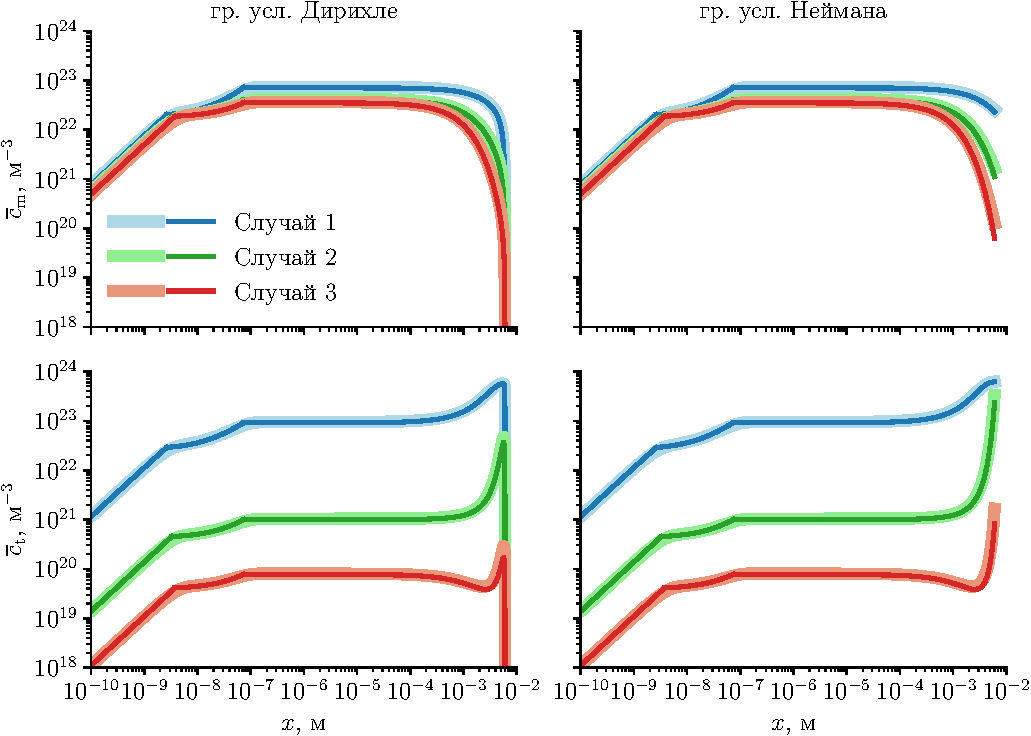
\includegraphics[scale=1]{retention_saturation.pdf}
	}
	\caption{Сравнение аналитических профилей концентрации дейтерия при насыщении (тонкие линии) с профилями, полученными на основе численных расчетов с использованием средних компонент потоков тепла и частиц (широкие линии)}\label{fig:ch3/retention_saturation}
\end{figure}


\section{Выводы к главе 3}
Проведено численное моделирование динамики захвата дейтерия в вольфрамовых элементах под действием импульсных плазменных нагрузок. Валидация модели выполнена путем воспроизведения экспериментальных ТДС-данных после облучения на установке КСПУ-Т, показавшего хорошее согласие в приближении ограниченной скорости десорбции.   

Для условий, соответствующих ELM-событиям в ИТЭР, расчеты демонстрируют снижение скорости накопления дейтерия в широком диапазоне параметров. Этот эффект обусловлен дополнительным нагревом материала из-за воздействия высокоэнергетичных частиц и более выражен при высокой частоте ELM-событий на фоне умеренных базовых нагрузок. Было выявлено несколько факторов (ограниченная скорость десорбции, наличие центров захвата с большим барьером освобождения), способных повысить скорость накопления во время ELM-событий. С другой стороны, нагрев материала до высоких температур во время переходных процессов обеспечивает условия для более быстрой диффузии в объем, что может влиять на время проникновения изотопов водорода (в том числе трития) в систему охлаждения ОПЭ и на эффективность последующего обезгаживания между экспериментальными кампаниями. В силу этого, ранние оценки содержания при базовых сценариях разрядов в ИТЭР без учета влияния ELM-событий могут быть завышенными. 

В приближении малых амплитуд импульсных нагрузок во время ELM-событий была продемонстрирована возможность использования только средних компонент для получения быстрых оценок содержания. Были получены аналитические выражения, определяющие квазистационарное распределения дейтерия в приближении точечных источников подвижных атомов при наличии центров захвата и градиента температуры. Аналитические выражения хорошо согласуются с результатами численных расчетов и могут быть использованы для оценки содержания дейтерия при насыщении.

\nomenclature[A]{FSM}{Модель <<свободного потока>> (Free streaming model)}
\nomenclature[P, 53]{\( T_{\mathrm{e,t}} \)}{Температура электронов вблизи мишени дивертора, \si{\electronvolt}}
\nomenclature[P, 53]{\( \gamma \)}{Коэффициент пропорциональности между потоками тепла и частиц, приходящими на поверхность (sheath heat transmission factor)}
\nomenclature[P, 64]{\( Q_\mathrm{fus} \)}{Отношение произведенной энергии за счет реакции термоядерного синтеза к вложенной}

\clearpage
           % Глава 3
\chapter*{Заключение}                       % Заголовок
\addcontentsline{toc}{chapter}{Заключение}  % Добавляем его в оглавление

%% Согласно ГОСТ Р 7.0.11-2011:
%% 5.3.3 В заключении диссертации излагают итоги выполненного исследования, рекомендации, перспективы дальнейшей разработки темы.
%% 9.2.3 В заключении автореферата диссертации излагают итоги данного исследования, рекомендации и перспективы дальнейшей разработки темы.
%% Поэтому имеет смысл сделать эту часть общей и загрузить из одного файла в автореферат и в диссертацию:

%% Согласно ГОСТ Р 7.0.11-2011:
%% 5.3.3 В заключении диссертации излагают итоги выполненного исследования, рекомендации, перспективы дальнейшей разработки темы.
%% 9.2.3 В заключении автореферата диссертации излагают итоги данного исследования, рекомендации и перспективы дальнейшей разработки темы.
В рамках данной диссертационной работы методом численного моделирования были исследованы закономерности захвата и десорбции дейтерия в вольфраме при импульсных плазменном и лазерном воздействии. Среди наиболее значимых результатов можно выделить следующие:
\begin{enumerate}
  \item В программном пакете FESTIM была реализована модель, учитывающая кинетику процессов на поверхности. Реализованная модель расширяет функциональные возможности кода, что подтверждено в ходе проверки корректности ее имплементации. Модель включена в состав свободно распространяемого программного обеспечения и доступна всем пользователям.
  \item Сравнение результатов моделирования с экспериментальными данными по захвату дейтерия в вольфраме при импульсном плазменном облучении и экспериментами по ЛИД дейтерия из вольфрамовых пленок показало хорошее соответствие, что подтверждает применимость стандартных моделей для анализа динамики транспорта дейтерия при импульсных нагрузках.
  \item На основе численного моделирования проведен комплексный анализ влияния импульсно-периодических плазменных нагрузок, соответствующих ELM-событиям в крупных токамаках, на долговременное накопление дейтерия в вольфраме. Установлено, что в широком диапазоне параметров облучения скорость накопления дейтерия в переходных процессах снижается вследствие существенного нагрева материала высокоэнергетичными частицами. Эффект усиливается с ростом частоты импульсных нагрузок. 
  \item Показано, что дополнительный нагрев во время переходных процессов способствует более глубокому проникновению дейтерия. Данный эффект усиливается с увеличением частоты импульсных нагрузок, приводящих к росту средней температуры материала. В условиях термоядерных установок это может влиять как на скорость проникновения изотопов водорода в систему охлаждения, так и на эффективность дегазации элементов установки между плазменными кампаниями.
  \item В приближении малых импульсных нагрузок во время переходных событий построена аналитическая модель, описывающая квазистационарное распределение дейтерия в материале с учетом влияния центров захвата и градиента температур. Развитая модель может быть использована для оценки предельного уровня содержания изотопов водорода в квазистационарном режиме при достижении насыщения.
  \item Проведен детальный численный анализ состава потока десорбированных частиц при ЛИД. Установлено, что вероятность прямой десорбции атомов увеличивается с ростом температуры поверхности и уменьшением полного потока выходящих частиц. Условия для десорбции атомов могут быть выполнены при использовании лазерных импульсов с длительностью от \SI{10}{\micro\second}. В рамках подхода получена оценка атомарной фракции на уровне \( \sim \SI{10}{\percent} \) в случае использования лазерных импульсов с миллисекундной длительностью, что может вносить дополнительную погрешность при проведении оценки содержания изотопов водорода.
  \item Исследована эффективность анализа содержания дейтерия методом ЛИД в широком диапазоне параметров материала и лазерного облучения. Наибольшая эффективность достигается при использовании более длительных лазерных импульсов. Показано, что измерение температуры поверхности позволяет снизить влияние неопределенности теплофизических свойств материала на точность измерений. Основным источником погрешности является неопределенность энергетического барьера выхода из центров захвата, тогда как влияние концентрации центров захвата оказывается менее значительным.    
\end{enumerate}

      % Заключение
\printnomenclature[3.5cm] % Значение ширины столбца с обозначениями стоит подбирать вручную
        % Список сокращений и условных обозначений
\chapter*{Словарь терминов}             % Заголовок
\addcontentsline{toc}{chapter}{Словарь терминов}  % Добавляем его в оглавление

\textbf{ТЯУ} : Термоядерная установка

\textbf{ОПЭ} : Обращенные к плазме элементы

\textbf{ОПМ} : Обращенные к плазме материалы

\textbf{МКЭ} : Метод конечных элементов

\textbf{ТДС} : Термодесорбционная спектроскопия

\textbf{ЛИД} : Лазерно-индуцированная десорбция

\textbf{ИТЭР} : Международный экспериментальный термоядерный реактор ИТЭР

\textbf{ELM} : Edge localised modes (моды, локализованные на периферии)
      % Словарь терминов
\clearpage                                  % В том числе гарантирует, что список литературы в оглавлении будет с правильным номером страницы
%\hypersetup{ urlcolor=black }               % Ссылки делаем чёрными
%\providecommand*{\BibDash}{}                % В стилях ugost2008 отключаем использование тире как разделителя
\urlstyle{rm}                               % ссылки URL обычным шрифтом
\ifdefmacro{\microtypesetup}{\microtypesetup{protrusion=false}}{} % не рекомендуется применять пакет микротипографики к автоматически генерируемому списку литературы
% \insertbibliofull                           % Подключаем Bib-базы: все статьи единым списком
% Режим с подсписками
\insertbiblioexternal                      % Подключаем Bib-базы: статьи, не являющиеся статьями автора по теме диссертации
% Для вывода выберите и расскомментируйте одно из двух
\insertbiblioauthor                        % Подключаем Bib-базы: работы автора единым списком 
%\insertbiblioauthorgrouped                 % Подключаем Bib-базы: работы автора сгруппированные (ВАК, WoS, Scopus и т.д.)
\ifdefmacro{\microtypesetup}{\microtypesetup{protrusion=true}}{}
\urlstyle{tt}                               % возвращаем установки шрифта ссылок URL
%\hypersetup{ urlcolor={urlcolor} }          % Восстанавливаем цвет ссылок
      % Список литературы
\clearpage
\ifdefmacro{\microtypesetup}{\microtypesetup{protrusion=false}}{} % не рекомендуется применять пакет микротипографики к автоматически генерируемым спискам
\listoffigures  % Список изображений

%%% Список таблиц %%%
% (ГОСТ Р 7.0.11-2011, 5.3.10)
\clearpage
\listoftables   % Список таблиц
\ifdefmacro{\microtypesetup}{\microtypesetup{protrusion=true}}{}
\newpage           % Списки таблиц и изображений (иллюстративный материал)

\setcounter{totalchapter}{\value{chapter}} % Подсчёт количества глав

%%% Настройки для приложений
\appendix
% Оформление заголовков приложений ближе к ГОСТ:
\setlength{\midchapskip}{20pt}
\renewcommand*{\afterchapternum}{\par\nobreak\vskip \midchapskip}
\renewcommand\thechapter{\Asbuk{chapter}} % Чтобы приложения русскими буквами нумеровались

\chapter{Аналитические выражения для температурной зависимости теплофизических свойств материалов}\label{app:A}

Температурная зависимость теплофизических свойств материалов задавалась на основе полиномиальных выражений. Далее плотность материала \( \rho \) представлена в \si{\kilogram\per\meter\cubed}, удельная теплоемкость \( C_p \) "--- в \si{\joule\per\kilogram\per\kelvin}, теплопроводность \( \kappa \) "--- в \si{\watt\per\meter\per\kelvin}. Изменением плотности материала за счет расширения при нагреве во всех случаях пренебрегалось. Для вольфрама использовались функциональные зависимости, рекомендованные Толиасом~\cite{Tolias2017} на основе критического анализа литературных данных:
\begin{subequations}
    \label{eq:app/W_props}
    \begin{align}
        \rho  =             & \num{19250},                                                                   \\
        C_p M_\mathrm{W}  = & \left\{
        \begin{alignedat}{3}
            & \num{21.868372} + \num{8.068661e-3} T - \num{3.756196e-6} T^2 +     \\
            & + \num{1.075862e-9} T^3 + \num{1.406637e4} T^{-2}, \quad \SI{300}{\kelvin} \leq T \leq \SI{3080}{\kelvin}, \\
            & \num{2.022} + \num{1.315e-3} T, \quad \SI{3080}{\kelvin} \textless T \leq \SI{3695}{\kelvin},
        \end{alignedat}
        \right.                                                                                              \\
        \kappa =            & \num{149.441} - \num{45.466e-3} T + \num{13.193e-6} T^2 - \num{1.484e-9} T^3 + \\
                            & + \num{3.866e6} T^{-2}, \nonumber
    \end{align}
\end{subequations}
где \( T \) "--- температура, \si{\kelvin}; \( M_\mathrm{W}=\SI{183.84e-3}{\kilogram\per\mole} \) "--- молярная масса вольфрама.

\begin{comment}
Для бериллия использовались функциональные зависимости, рекомендованные Толиасом~\cite{Tolias2022} на основе критического анализа литературных данных. Изменением теплофизических свойств при переходе из альфа- в бета-фазу пренебрегалось:
\begin{subequations}
    \label{eq:app/Be_props}
    \begin{align}
        \rho              & =  \num{1850},                                                                         \\
        C_p M_\mathrm{Be} & =  \num{21.205} + \num{5.694e-3} T + \num{0.962e-6} T^2 - \num{0.5874e6} T^{-2},       \\
        \kappa            & =  \num{148.8912} - \num{76.3780e-3} T + \num{12.0174e-6} T^2 + \num{6.5407e6} T^{-2},
    \end{align}
\end{subequations}
где \( M_\mathrm{Be}=\SI{9.012e-3}{\kilogram\per\mole} \) "--- молярная масса бериллия.
\end{comment}

Функциональные зависимости для меди и сплава бронзы (CuCrZr) были выбраны на основе работы Ван ден Керкхофа и др.~\cite{VandenKerkhof2021}, которые получили аналитические зависимости на основе данных из внутреннего отчета Международной организации ИТЭР~\cite{komarov2013thermal}. Зависимости для меди определены следующим образом:
\begin{subequations}
    \label{eq:app/Cu_props}
    \begin{align}
        \rho   & =  \num{8960},                                                             \\
        C_p    & =  \num{3.71e2} + \num{4.59e-2} T + \num{3.85e-5} T^2 ,                    \\
        \kappa & =  \num{4.18e2} - \num{4.75e-2} T - \num{4.81e-5} T^2 + \num{3.09e-8} T^3.
    \end{align}
\end{subequations}

Соответствующие зависимости для сплава бронзы:
\begin{subequations}
    \label{eq:app/CuCrZr_props}
    \begin{align}
        \rho   & =  \num{8940},                                                             \\
        C_p    & =  \num{3.63e2} + \num{8.96e-2} T + \num{7.58e-6} T^2 ,                    \\
        \kappa & = \num{1.84e2} + \num{7.28e-1} T - \num{1.08e-3} T^2 +  \num{5.26e-7} T^3.
    \end{align}
\end{subequations}

\chapter{Значения физических параметров для проведения моделирования}\label{app:B}

\begin{table}[ht]
    \centering
    \begin{threeparttable}
        \caption{Параметры моделирования для первого валидационного теста}
        \label{tab:case1_inputs}
        \renewcommand{\arraystretch}{1.2}%% Увеличение расстояния между рядами, для улучшения восприятия.
        \begin{tabularx}{\textwidth}{@{}>{\raggedright}Xcc}
            \toprule
            Наименование                                                                                                                    & Обозначение           & Значение       \\
            \hline
            \hline
            Толщина области, \si{\meter}                                                                                                    & $L$                   & \num{1.0e-3}   \\
            Концентрация атомов решетки титана,~\si{\per\meter\cubed}                                                                       & $n_\mathrm{Ti}$       & \num{5.66e28}  \\
            Концентрация межузельных положений,~\si{\per\meter\cubed}                                                                       & $n_\mathrm{IS}$       & \num{1.69e29}  \\
            Концентрация адсорбционных положений,~\si{\per\meter\squared}                                                                   & $n_\mathrm{s}$        & \num{3.90e19}  \\
            Расстояние между межузельными положениями,~\si{\meter}                                                                          & $\lambda_\mathrm{IS}$ & \num{2.29e-10} \\
            Предэкспоненциальный множитель коэффициента диффузии,~\si{\meter\squared\per\second}                                            & $D_0$                 & \num{9.0e-7}   \\
            Энергия активации диффузии,~\si{\electronvolt}                                                                                  & $E_\mathrm{D}$        & \num{0.538}    \\
            Энергия активации десорбции,~\si{\electronvolt}                                                                                 & $E_\mathrm{des}$      & \num{0.562}    \\
            Энергия активации перехода из растворенного состояния в адсорбированное,~\si{\electronvolt}                                     & $E_\mathrm{bs}$       & \num{1.052}    \\
            Энергия активации перехода из адсорбированного состояния в растворенное,~\si{\electronvolt}                                     & $E_\mathrm{sb}$       & \num{1.009}    \\
            Энергия активации диссоциативной адсорбции,~\si{\electronvolt}                                                                  & $E_\mathrm{diss}$     & \num{2.06e-2}  \\
            Предэкспоненциальный множитель коэффициента прилипания                                                                          & $\Phi_0$              & \num{1.43e-2}  \\
            Предэкспоненциальный множитель константы скорости десорбции,~\si{\meter\squared\per\second}                                     & $\nu_\mathrm{des,0}$  & \num{3.41e-11} \\
            Предэкспоненциальный множитель константы скорости перехода из растворенного состояния в адсорбированное,~\si{\meter\per\second} & $\nu_\mathrm{bs,0}$   & \num{2.3}      \\
            Предэкспоненциальный множитель константы скорости перехода из адсорбированного состояния в растворенное,~\si{\per\second}       & $\nu_\mathrm{sb,0}$   & \num{5.14e9}   \\
            Начальное давление,~\si{\pascal}                                                                                                & $P_\mathrm{H_2,0}$    & \num{1.3e4}    \\
            Объем камеры,~\si{\meter\cubed}                                                                                                 & $V_\mathrm{ch}$       & \num{2.95e-3}  \\
            \bottomrule
        \end{tabularx}
    \end{threeparttable}
\end{table}

\begin{table}[t!]
    \centering
    \begin{threeparttable}
        \caption{Параметры моделирования для второго валидационного теста}
        \label{tab:case2_inputs}
        \renewcommand{\arraystretch}{1.2}%% Увеличение расстояния между рядами, для улучшения восприятия.
        \begin{tabularx}{\textwidth}{@{}>{\raggedright}Xcc}
            \toprule
            Наименование                                                                                                & Обозначение           & Значение                     \\
            \hline
            \hline
            Толщина области, \si{\meter}                                                                                & $L$                   & \num{2,0e-3}                 \\
            Концентрация атомов решетки вольфрама,~\si{\per\meter\cubed}                                                & $n_\mathrm{W}$        & \num{6.3382e28}              \\
            Концентрация межузельных положений,~\si{\per\meter\cubed}                                                   & $n_\mathrm{IS}$       & \num{3.8029e29}              \\
            Концентрация адсорбционных положений на чистой поверхности ($\theta_\mathrm{O}=0$),~\si{\per\meter\squared} & $n_\mathrm{s}$        & \num{1.416e19}               \\
            Расстояние между межузельными положениями,~\si{\meter}                                                      & $\lambda_\mathrm{IS}$ & \num{1.117e-10}              \\
            Частота тепловых колебаний атомов,~\si{\per\second}                                                         & $\nu_0$               & \num{e13}                    \\
            Предэкспоненциальный множитель коэффициента диффузии,~\si{\meter\squared\per\second}                        & $D_0$                 & \num{1.365e-7}               \\
            Энергия активации диффузии,~\si{\electronvolt}                                                              & $E_\mathrm{D}$        & \num{0.2}                    \\
            Энергия активации десорбции,~\si{\electronvolt}                                                             & $E_\mathrm{des}$      & ур.~\cref{eq:ch2/case2_Edes} \\
            Энергия активации перехода из растворенного состояния в адсорбированное,~\si{\electronvolt}                 & $E_\mathrm{bs}$       & \num{0.2}                    \\
            Энергия активации перехода из адсорбированного состояния в растворенное,~\si{\electronvolt}                 & $E_\mathrm{sb}$       & ур.~\cref{eq:ch2/case2_Esb}  \\
            Энергия активации диссоциативной адсорбции,~\si{\electronvolt}                                              & $E_\mathrm{diss} $    & 0                            \\
            Теплота растворения,~\si{\electronvolt}                                                                     & $Q_\mathrm{s}$        & 1                            \\
            Предэкспоненциальный множитель коэффициента прилипания                                                      & $\Phi_0$              & 1                            \\
            Начальное давление,~\si{\pascal}                                                                            & $P_\mathrm{D_2}$      & \num{2e-5}                   \\
            \bottomrule
        \end{tabularx}
    \end{threeparttable}
\end{table}

\begin{table}[t!]
    \centering
    \begin{threeparttable}
        \caption{Параметры, определяющие функциональную зависимость энергии активации десорбции от степени покрытия поверхности вольфрама дейтерием}
        \label{tab:case2_Edes_params}
        \renewcommand{\arraystretch}{1.2}%% Увеличение расстояния между рядами, для улучшения восприятия.
        \begin{tabularx}{\textwidth}{>{\centering\arraybackslash}X>{\centering\arraybackslash}X>{\centering\arraybackslash}X>{\centering\arraybackslash}X>{\centering\arraybackslash}X>{\centering\arraybackslash}X>{\centering\arraybackslash}X}
            \toprule
            {\(\theta_{\mathrm{O}}\)} & {$E_0$,~\si{\electronvolt}} & {$\Delta E$,~\si{\electronvolt}} & {$\theta_\mathrm{D,0}$} & {$\delta\theta_\mathrm{D}$} & {a}   & {b}   \\
            \hline
            \hline
            0.00                      & 1.142                       & 0.346                            & 0.253                   & 0.180                       & 0.303 & 8.902 \\
            0.50                      & 1.111                       & 0.289                            & 0.113                   & 0.082                       & 0.460 & 7.240 \\
            0.75                      & 1.066                       & 0.234                            & 0.161                   & 0.057                       & 0.437 & 4.144 \\
            \bottomrule
        \end{tabularx}
    \end{threeparttable}
\end{table}

\begin{table}[t!]
    \centering
    \begin{threeparttable}
        \caption{Параметры моделирования для третьего валидационного теста}
        \label{tab:case3_inputs}
        \renewcommand{\arraystretch}{1.2}%% Увеличение расстояния между рядами, для улучшения восприятия.
        \begin{tabularx}{\textwidth}{@{}>{\raggedright}Xcc}
            \toprule
            Наименование                                                                                & Обозначение           & Значение        \\
            \hline
            \hline
            Толщина области, \si{\meter}                                                                & $L$                   & \num{0.800e-3}  \\
            Концентрация атомов решетки вольфрама,~\si{\per\meter\cubed}                                & $n_\mathrm{W}$        & \num{6.300e28}  \\
            Концентрация межузельных положений,~\si{\per\meter\cubed}                                   & $n_\mathrm{IS}$       & \num{3.780e29}  \\
            Концентрация адсорбционных положений,~\si{\per\meter\squared}                               & $n_\mathrm{s}$        & \num{1.090e20}  \\
            Расстояние между межузельными положениями,~\si{\meter}                                      & $\lambda_\mathrm{IS}$ & \num{1.100e-10} \\
            Частота тепловых колебаний атомов,~\si{\per\second}                                         & $\nu_0$               & \num{1.000e13}  \\
            Предэкспоненциальный множитель коэффициента диффузии,~\si{\meter\squared\per\second}        & $D_0$                 & \num{1.365e-7}  \\
            Энергия активации диффузии,~\si{\electronvolt}                                              & $E_\mathrm{D}$        & \num{0.200}     \\
            Энергия активации десорбции,~\si{\electronvolt}                                             & $E_\mathrm{des}$      & \num{1.740}     \\
            Энергия активации перехода из растворенного состояния в адсорбированное,~\si{\electronvolt} & $E_\mathrm{bs}$       & \num{0.200}     \\
            Энергия активации перехода из адсорбированного состояния в растворенное,~\si{\electronvolt} & $E_\mathrm{sb}$       & \num{1.545}     \\
            Энергия активации диссоциативной адсорбции,~\si{\electronvolt}                              & $E_\mathrm{diss}$     & \num{0.63}      \\
            Коэффициент прилипания                                                                      & $\Phi$                & \num{0.190}     \\
            Плотность потока атомов,~\si{\per\meter\squared\per\second}                                 & $\Gamma_\mathrm{D}$   & \num{5.800e18}  \\
            Сечение рекомбинации Или-Ридила,~\si{\meter\squared}                                        & $\sigma_\mathrm{ER}$  & \num{1.700e-21} \\
            \bottomrule
        \end{tabularx}
    \end{threeparttable}
\end{table}

\begin{table}[t!]
    \centering
    \begin{threeparttable}
        \caption{Параметры центров захвата для третьего валидационного теста}
        \label{tab:case3_traps_params}
        \renewcommand{\arraystretch}{1.2}%% Увеличение расстояния между рядами, для улучшения восприятия.
        \begin{tabularx}{\textwidth}{>{\centering\arraybackslash}X>{\centering\arraybackslash}X>{\centering\arraybackslash}X>{\centering\arraybackslash}X>{\centering\arraybackslash}X>{\centering\arraybackslash}X}
            \toprule
            Тип дефекта & $n_\mathrm{t}$,~ат.\% & $E_\mathrm{dt}$,~\si{\electronvolt} & $\nu_\mathrm{dt,0}$,~\si{\per\second} & $E_\mathrm{t}$,~\si{\electronvolt} & $\nu_\mathrm{t,0}$,~\si{\meter\cubed\per\second} \\
            \hline
            \hline
            1           & \num{0.01}            & \num{0.85}                          & \multirow{5}{*}{\num{e13}}            & \multirow{5}{*}{\num{0.2}}         & \multirow{5}{*}{\num{2.98e-17}}                  \\
            2           & \num{0.01}            & \num{1.00}                          &                                       &                                    &                                                  \\
            3           & \num{0.19}            & \num{1.65}                          &                                       &                                    &                                                  \\
            4           & \num{0.16}            & \num{1.85}                          &                                       &                                    &                                                  \\
            5           & \num{0.02}            & \num{2.06}                          &                                       &                                    &                                                  \\
            \bottomrule
        \end{tabularx}
    \end{threeparttable}
\end{table}

\begin{table}[t!]
    \centering
    \begin{threeparttable}
        \caption{Параметры моделирования для четвертого валидационного теста}
        \label{tab:case4_inputs}
        \renewcommand{\arraystretch}{1.2}%% Увеличение расстояния между рядами, для улучшения восприятия.
        \begin{tabularx}{\textwidth}{@{}>{\raggedright}Xcc}
            \toprule
            Наименование                                                                                                                    & Обозначение                           & Значение        \\
            \hline
            \hline
            Толщина области, \si{\meter}                                                                                                    & $L$                                   & \num{0.800e-3}  \\
            Концентрация атомов решетки вольфрама,~\si{\per\meter\cubed}                                                                    & $n_\mathrm{EFe}$                      & \num{8.59e28}   \\
            Концентрация межузельных положений,~\si{\per\meter\cubed}                                                                       & $n_\mathrm{IS}$                       & \num{5.15e29}   \\
            Концентрация адсорбционных положений,~\si{\per\meter\squared}                                                                   & $n_\mathrm{s}$                        & \num{1.947e20}  \\
            Расстояние между межузельными положениями,~\si{\meter}                                                                          & $\lambda_\mathrm{IS}$                 & \num{2.266e-10} \\
            Предэкспоненциальный множитель коэффициента диффузии,~\si{\meter\squared\per\second}                                            & $D_0$                                 & \num{1.5e-7}    \\
            Энергия активации диффузии,~\si{\electronvolt}                                                                                  & $E_\mathrm{D}$                        & \num{0.15}      \\
            Энергия активации десорбции,~\si{\electronvolt}                                                                                 & $E_\mathrm{des}$                      & \num{0.63}      \\
            Энергия активации перехода из растворенного состояния в адсорбированное,~\si{\electronvolt}                                     & $E_\mathrm{bs}$                       & \num{0.200}     \\
            Энергия активации диссоциативной адсорбции,~\si{\electronvolt}                                                                  & $E_\mathrm{diss}$                     & \num{0.4}       \\
            Теплота растворения,~\si{\electronvolt}                                                                                         & $Q_\mathrm{s}$                        & \num{0.238}     \\
            Предэкспоненциальный множитель коэффициента прилипания                                                                          & $\Phi_0$                              & \num{e-4}       \\
            Предэкспоненциальный множитель растворимости,~\si{\per\meter\cubed\per\pascal}$^{-0.5}$                                         & $K_{\mathrm{S},0}$                    & \num{1.319e23}  \\
            Предэкспоненциальный множитель константы скорости перехода из растворенного в адсорбированное состояние,~\si{\meter\per\second} & $\nu_{\mathrm{bs},0}$                 & \num{661.844}   \\
            Предэкспоненциальный множитель константы скорости десорбции,~\si{\meter\squared\per\second}                                     & $\nu_{\mathrm{des},0}^{\mathrm{D_2}}$ & \num{661.844}   \\
            Плотность потока атомов,~\si{\per\meter\squared\per\second}                                                                     & $\Gamma_\mathrm{D}$                   & \num{5.5e18}    \\
            Сечение рекомбинации Или-Ридила,~\si{\meter\squared}                                                                            & $\sigma_\mathrm{ER}$                  & \num{4.109e-15} \\
            Глубина внедрения,~\si{\meter}                                                                                                  & $X$                                   & \num{-e-10}     \\
            Стандартное отклонение профиля внедренных атомов,~\si{\meter}                                                                   & $\sigma$                              & \num{7.5e-10}   \\
            Коэффициент отражения                                                                                                           & $r$                                   & \num{0.612}     \\
            Начальное давление,~\si{\pascal}                                                                                                & $P_\mathrm{D_2}$                      & \num{1}         \\
            \bottomrule
        \end{tabularx}
    \end{threeparttable}
\end{table}

\begin{table}[t!]
    \centering
    \begin{threeparttable}
        \caption{Параметры центров захвата для четвертого валидационного теста}
        \label{tab:case4_traps_params}
        \renewcommand{\arraystretch}{1.2}%% Увеличение расстояния между рядами, для улучшения восприятия.
        \begin{tabularx}{\textwidth}{>{\centering\arraybackslash}X>{\centering\arraybackslash}X>{\centering\arraybackslash}X>{\centering\arraybackslash}X>{\centering\arraybackslash}X>{\centering\arraybackslash}X}
            \toprule
            Тип дефекта
             & $n_\mathrm{t}$,~ат.\%
             & $E_\mathrm{dt}$,~\si{\electronvolt}
             & $\nu_\mathrm{dt,0}$,~\si{\per\second}
             & $E_\mathrm{t}$,~\si{\electronvolt}
             & $\nu_\mathrm{t,0}$,~\si{\meter\cubed\per\second}      \\
            \hline
            \hline
            1
             & \num{1.0e-3}
             & \num{0.90}
             & \multirow{2}{*}{\num{4.00e13}}
             & \multirow{2}{*}{\num{0.15}}
             & \multirow{2}{*}{\num{5.67e-18}}                       \\
            2
             & \numrange{2.5}{5.0e-2}
             & \num{1.08}
             &                                                  &  & \\
            \bottomrule
        \end{tabularx}
    \end{threeparttable}
\end{table}

\begin{table}[ht]
    \centering
    \begin{threeparttable}
        \caption{Физические параметры для моделирования транспорта дейтерия в вольфраме}
        \label{tab:W_props}
        \renewcommand{\arraystretch}{1.2}%% Увеличение расстояния между рядами, для улучшения восприятия.
        \begin{tabularx}{\textwidth}{@{}>{\raggedright}Xcc}
            \toprule
            Наименование                                                                                     & Обозначение            & Значение                    \\
            \hline
            \hline
            Концентрация атомов решетки,~\si{\per\meter\cubed}                                               & $n_\mathrm{W}$         & \num{6.310e28}              \\
            Концентрация межузельных положений,~\si{\per\meter\cubed}                                        & $n_\mathrm{IS}$        & \num{3.786e29}              \\
            Концентрация адсорбционных положений,~\si{\per\meter\squared}                                    & $n_\mathrm{s}$         & \num{1.997e19}              \\
            Расстояние между межузельными положениями,~\si{\meter}                                           & $\lambda_\mathrm{IS}$  & \num{1.100e-10}             \\
            Расстояние между межузельным и адсорбционным положениями,~\si{\meter}                            & $\lambda_\mathrm{abs}$ & \num{5.275e-11}             \\
            Предэкспоненциальный множитель коэффициента диффузии,~\si{\meter\squared\per\second}             & $D_0$                  & \num{1.365e-7}              \\
            Частота тепловых колебаний атомов,~\si{\per\second}                                              & $\nu_0$                & \num{1.000e13}              \\
            Предэкспоненциальный множитель константы скорости захвата в дефект,~\si{\meter\cubed\per\second} & $\nu_{\mathrm{t},0}$   & \num{2.979e-17}             \\
            Предэкспоненциальный множитель константы скорости выхода из дефекта,~\si{\per\second}            & $\nu_{\mathrm{dt},0}$  & \num{1.000e13}              \\
            Предэкспоненциальный множитель константы скорости перехода из растворенного
            в адсорбированное состояние,~\si{\meter\per\second}                                              & $\nu_{\mathrm{bs},0}$  & \num{594.931}               \\
            Предэкспоненциальный множитель константы скорости перехода из адсорбированного
            в растворенное состояние,~\si{\per\second}                                                       & $\nu_{\mathrm{sb},0}$  & \num{1.000e13}              \\
            Энергия активации диффузии,~\si{\electronvolt}                                                   & $E_\mathrm{D}$         & \num{0.200}                 \\
            Теплота растворения,~\si{\electronvolt}                                                          & $Q_\mathrm{s}$         & \num{1.040}                 \\
            Энергия активации перехода из растворенного состояния в адсорбированное,~\si{\electronvolt}      & $E_\mathrm{bs}$        & \num{0.200}                 \\
            Энергия активации перехода из адсорбированного состояния в растворенное,~\si{\electronvolt}      & $E_\mathrm{sb}$        & $E_\mathrm{s}-Q_\mathrm{c}$ \\
            \bottomrule
        \end{tabularx}
    \end{threeparttable}
\end{table}

% \chapter{Физические параметры, использованные для моделирования транспорта дейтерия в вольфраме}\label{app:C}



\begin{comment}
\begin{table}[ht]
    \centering
    \begin{threeparttable}
        \caption{Физические параметры бериллия}
        \label{tab:Be_props}
        \renewcommand{\arraystretch}{1.2}%% Увеличение расстояния между рядами, для улучшения восприятия.
        \begin{tabularx}{\textwidth}{@{}>{\raggedright}Xcc}
            \toprule
            Наименование                                                                                & Обозначение            & Значение        \\
            \hline
            \hline
            Концентрация атомов решетки,~\si{\per\meter\cubed}                                          & $n_\mathrm{Be}$        & \num{1.230e28}  \\
            Концентрация межузельных положений,~\si{\per\meter\cubed}                                   & $n_\mathrm{IS}$        & \num{7.380e29}  \\
            Концентрация адсорбционных положений ,~\si{\per\meter\squared}                              & $n_\mathrm{s}$         & \num{2.473e19}  \\
            Расстояние между межузельными положениями,~\si{\meter}                                      & $\lambda_\mathrm{IS}$  & \num{3.154e-10} \\
            Расстояние между межузельным и адсорбционным положениями,~\si{\meter}                       & $\lambda_\mathrm{abs}$ & \num{3.351e-11} \\
            Частота тепловых колебаний атомов,~\si{\per\second}                                         & $\nu_0$                & \num{1.000e13}  \\
            Предэкспоненциальный множитель коэффициента диффузии,~\si{\meter\squared\per\second}        & $D_0$                  & \num{9.899e-7}  \\
            Энергия активации диффузии,~\si{\electronvolt}                                              & $E_\mathrm{D}$         & \num{0.380}     \\
            Энергия активации перехода из растворенного состояния в адсорбированное,~\si{\electronvolt} & $E_\mathrm{bs}$        & \num{0.380}     \\
            Энергия активации перехода из адсорбированного состояния в растворенное,~\si{\electronvolt} & $E_\mathrm{sb}$        & \num{2.460}     \\
            Теплота растворения,~\si{\electronvolt}                                                     & $Q_\mathrm{s}$         & \num{1.580}     \\
            Теплота хемосорбции,~\si{\electronvolt}                                                     & $|Q_\mathrm{c}|$       & \num{0.500}     \\
            Энергия активации растворения,~\si{\electronvolt}                                             & $E_\mathrm{s}$         & \num{1.960}     \\
            \bottomrule
        \end{tabularx}
    \end{threeparttable}
\end{table}
\end{comment}

\chapter{Параметры, определяющие температурную зависимость потока тепла через границу раздела W-Cu}\label{app:C}

\begin{table}[h]
    \renewcommand{\arraystretch}{1.25}
       \centering
    \rotatebox{270}{
    \begin{minipage}{0.9\textwidth}
        \small
        \caption{Подгоночные параметры в уравнениях~\cref{eq:ch3/heat_WCu}} \label{tab:fit_params}
        \begin{threeparttable}
            \begin{tabular}{*{13}c}
                \toprule
                $q_{\mathrm{stat}}$, & Параметр & \multicolumn{11}{l}{Частота ELM-событий, Гц} \\
                \cline{3-13} 	 
                \si{\mega\watt\per\meter\squared} && Стац. &10 & 20 & 30 & 40 & 50 & 60 & 70 & 80 & 90 & 100 \\
                \hline
                \hline
                1 & a, 1 	& 0.151 & 0.135 & 0.134 & 0.132 & 0.130 & 0.129 & 0.128 & 0.127 & 0.126 & 0.125 & 0.124\\
                & b, К$^{-1}$  & 0.063 & 0.012 & 0.009 & 0.008 & 0.007 & 0.006 & 0.006 & 0.005 & 0.005 & 0.005 & 0.005 \\
                & c, 1 		  & 0.145 & 0.122 & 0.126 & 0.125 & 0.124 & 0.123 & 0.122 & 0.121 & 0.120 & 0.120 & 0.119 \\
                & d, К 		  & 0.96  & 4.16  & 6.05 & 7.02  & 7.82  & 8.49  & 9.11  & 9.65  & 10.18  & 10.65 & 11.09 \\
                        
                5 & a, 1  		  & 0.139 & 0.131 & 0.128 & 0.126 & 0.125 & 0.124 & 0.123 & 0.123 & 0.122 & 0.121 & 0.121\\
                & b, К$^{-1}$  & 0.013 & 0.007 & 0.006 & 0.005 & 0.005 & 0.004 & 0.004 & 0.004 & 0.004 & 0.004 & 0.004 \\
                & c, 1 		  & 0.134 & 0.120 & 0.121 & 0.121 & 0.120 & 0.119 & 0.118 & 0.117 & 0.117 & 0.117 & 0.116 \\
                & d, К 		  & 4.29  & 8.20  & 9.00  & 9.83  & 10.57  & 11.22  & 11.81  & 12.36  & 12.88 & 13.34 & 13.78 \\
                            
                10& a, 1 	      & 0.130 & 0.124 & 0.123 & 0.121 & 0.121 & 0.120 & 0.119 & 0.119 & 0.119 & 0.118 & 0.118\\
                & b, К$^{-1}$  & 0.007 & 0.005 & 0.004 & 0.004 & 0.003 & 0.003 & 0.003 & 0.003 & 0.003 & 0.003 & 0.003 \\
                & c, 1 		  & 0.125 & 0.118 & 0.118 & 0.117 & 0.116 & 0.116 & 0.115 & 0.115 & 0.114 & 0.114 & 0.114 \\
                & d, К 		  & 7.81 & 11.79 & 12.31 & 13.09 & 13.82 & 14.48 & 15.08 & 15.64 & 16.17 & 16.66 & 17.14 \\
                \bottomrule
            \end{tabular}
        \end{threeparttable}
    \end{minipage}}
\end{table}


\chapter{Решение стационарного уравнения диффузии с учетом градиента температуры}\label{app:D}

Рассмотрим стационарное уравнение диффузии с известным распределением температуры ($\partial_x T \neq 0$), определенное на отрезке \( x \in [0, L] \). На левой границе зададим однородное граничное условие Дирихле, когда на правой рассмотрим два случая: однородное условие Дирихле и однородное условие Неймана. Сначала обобщим уравнение~\eqref{eq:ch3/eq:solute_analytic} на случай $k$ источников:
\begin{align}
	\label{eq:general_stat_dif}
	\begin{cases}
		\dfrac{\partial}{\partial x}\left( D(T)\left[ \dfrac{\partial c}{\partial x} + H(T)c\right]\right)=-\sum\limits_{i=1}^k S_i(x), \\[5pt]
		\left.c\right\vert_{x=0}=0,                                                                                                     \\[5pt]
		\left[\begin{array}{ll}
			      \left.c\right\vert_{x=L}=0,  \text{если гр. усл. Дирихле}, \\[5pt]
			      \left.D(T)\left( \dfrac{\partial c}{\partial x} + H(T)c\right)\right\vert_{x=L}=0,  \text{если гр. усл. Неймана}.
		      \end{array}
		\right.
	\end{cases}
\end{align}
По сравнению с уравнением~\eqref{eq:ch3/eq:solute_analytic}, обозначения сокращены для краткости. Уравнение диффузии может быть сведено к:
\begin{equation}
	\frac{\partial}{\partial x}\left(p(x)\frac{\partial}{\partial x}\left[ ce^{\int\limits_0^x H(T)d\chi}\right]\right)=-\sum\limits_{i=1}^k S_i(x),
\end{equation}
где $p(x)=D(T)e^{-\int\limits_0^x H(T)d\chi}$. Решение этого уравнения можно найти, применив теорему суперпозиции:
\begin{equation}
	\label{eq:ST}
	c=e^{-\int\limits_0^x H(T)d\chi}\,\sum\limits_{i=1}^k \left( \int\limits_0^L G(x,y)S_i(y)dy \right),
\end{equation}
где $G(x,y)$ является функцией Грина, удовлетворяющей следующей вспомогательной задаче:
\begin{align}
	\label{eq:Green_problem}
	\begin{cases}
		\dfrac{\partial}{\partial x}\left(p(x)\,\dfrac{\partial G(x,y)}{\partial x}\right)=-\delta(x-y), \\[5pt]
		\left.G(x,y)\right\vert_{x=0}=0,                                                                 \\[5pt]
		\left[\begin{array}{ll}
			      \left.G(x,y)\right\vert_{x=L}=0,  \text{eсли гр. усл. Дирихле}, \\[5pt]
			      \left.p(x)\,\dfrac{\partial G(x,y)}{\partial x}\right\vert_{x=L}=0,  \text{eсли гр. усл. Неймана},
		      \end{array}\right.
	\end{cases}
\end{align}
где \( \delta(x) \) "--- дельта-функция Дирака. В особой точке выполняются свойства функции Грина краевой задачи:
\begin{gather}
	\label{eq:Green_problem_connect}
	 \left.G(x,y)\right\vert_{x=y^+}=\left.G(x,y)\right\vert_{x=y^-},                                                                                   \\
	 \left.p(x)\,\dfrac{\partial G(x,y)}{\partial x}\right\vert_{x=y^+}-\left.p(x)\,\dfrac{\partial G(x,y)}{\partial x}\right\vert_{x=y^-}=-1.\nonumber
\end{gather}

Для обоих типов условий на правой границе функция Грина может быть выражена следующим образом:
\begin{subequations}
	\label{eq:Green_solution}
	\begin{align}
		 & \text{Если гр. усл. Дирихле}:
		\begin{cases}
			G_1(x,y)=\int\limits_0^x\dfrac{d\chi}{p(\chi)}\,\dfrac{\int\limits_y^L\dfrac{d\chi}{p(\chi)}}{\int\limits_0^L\dfrac{d\chi}{p(\chi)}}, & x\in[0,y], \\[25pt]
			G_2(x,y)=\int\limits_0^y\dfrac{d\chi}{p(\chi)}\,\dfrac{\int\limits_x^L\dfrac{d\chi}{p(\chi)}}{\int\limits_0^L\dfrac{d\chi}{p(\chi)}}, & x\in[y,L]. \\
		\end{cases}\label{eq:Green_solution_D} \\[10pt]
		 & \text{Если гр. усл. Неймана}:
		\begin{cases}
			G_1(x,y)=\int\limits_0^x\dfrac{d\chi}{p(\chi)}, & x\in[0,y], \\[10pt]
			G_2(x,y)=\int\limits_0^y\dfrac{d\chi}{p(\chi)}, & x\in[y,L].
		\end{cases}\label{eq:Green_solution_N}
	\end{align}
\end{subequations}
Если градиент температуры мал ($\partial_x T \rightarrow 0$, $T \rightarrow$ const.), функция Грина сводится к:
\begin{subequations}
	\begin{align}
		 & \text{Если гр. усл. Дирихле}:
		\begin{cases}
			G_1(x,y)=\dfrac{x}{D(T)}\,\dfrac{L-y}{L}, & x\in[0,y], \\[25pt]
			G_2(x,y)=\dfrac{y}{D(T)}\,\dfrac{L-x}{L}, & x\in[y,L], \\
		\end{cases} \\[10pt]
		 & \text{Если гр. усл. Неймана}:
		\begin{cases}
			G_1(x,y)=\dfrac{x}{D(T)}, & x\in[0,y], \\[10pt]
			G_2(x,y)=\dfrac{y}{D(T)}, & x\in[y,L],
		\end{cases}
	\end{align}
\end{subequations}
что в точности соответствует выражениям, полученным ранее~\cite{Denis2022}. Подстановка уравнения~\eqref{eq:Green_solution} в выражение~\eqref{eq:ST} позволяет получить общее решение стационарной задачи диффузии:
\begin{align}
	c= & e^{-\int\limits_0^x H(T)d\chi}\,\sum\limits_{i=1}^k \left( \int\limits_0^x G_2(x,y)S_i(y)dy + \int\limits_x^L G_1(x,y)S_i(y)dy \right).\nonumber
\end{align}

\chapter{Решение уравнения теплопроводности на полубесконечной прямой}\label{app:E}

Уравнение теплопроводности, определяемое на полубесконечной прямой, описывается следующим образом:
\begin{align}
	\label{eq:heat_transfer_semiinfinite}
	\begin{cases}
		\dfrac{\partial T}{\partial t} & = a^2 \dfrac{\partial^2 T}{\partial x^2}, \\[5pt]
		\left.\dfrac{\partial T}{\partial x}\right\vert_{x=0}& = -\dfrac{q(t)}{\kappa},                \\[5pt]
        \left. T \right\vert_{t=0} & = T_0,
	\end{cases}
\end{align}
где \( a = \sqrt{\kappa/C_p\rho} \) "--- температуропроводность. Дифференциальное уравнение в частных производных определено на области \( x \geq 0 \). Тепловые свойства материала предполагаются не зависящими от температуры. Известно, что функция Грина для системы~\cref{eq:heat_transfer_semiinfinite} и изменение температуры за счет плотности потока на границе равны~\cite{Bechtel1975}:
\begin{subequations}
    \begin{gather}
        G(x,t|x',t') = \frac{1}{2a\sqrt{\pi(t-t')}} \left[ \exp \left( -\frac{(x-x')^2}{4a^2(t-t')} \right) + \exp \left( -\frac{(x+x')^2}{4a^2(t-t')} \right) \right],\label{eq:heat_eq_Green}\\
        T(x,t)-T_0 \equiv \Delta T(x,t) = \frac{a^2}{\kappa} \int\limits_0^t G(x,t|0,t')q(t')dt'. \label{eq:deltaT}
    \end{gather}
\end{subequations}
Подставляя функцию Грина~\cref{eq:heat_eq_Green} в уравнение~\cref{eq:deltaT} и полагая \(x=0\), приходим к выражению для временной эволюции изменения температуры поверхности:
\begin{equation}
    \Delta T(0,t) = \frac{1}{\sqrt{\pi\kappa C_p \rho}} \int\limits_0^t \frac{q(t')}{\sqrt{t-t'}}dt'.
\end{equation}

Для использованных временных профилей лазерных импульсов интеграл может быть сведен к табулированным трансцендентным функциям. Временной профиль при наносекундном нагреве явно задавался в соответствии с распределением Гаусса:
\begin{equation}
    q_\mathrm{ns}=\frac{E_0}{\sqrt{2\pi}\sigma_\tau} \exp \left( -\frac{(t-t_0)^2}{2\sigma_\tau^2} \right).
\end{equation} 
Повышение температуры поверхности при такой нагрузке~\cite{Bechtel1975}:
\begin{equation}
    \label{eq:dT_ns}
    \Delta T_\mathrm{ns}(0,t) = \frac{E_0}{\sqrt{2\pi\sigma_\tau \kappa C_p \rho}} \exp \left( -\frac{z^2}{4} \right) D_{-1/2}(-z),
\end{equation}
где \( z = (t-t_0)/\sigma_\tau \), \(D_{-1/2}(x) \) "--- функция параболического цилиндра. Дифференцируя выражение~\cref{eq:dT_ns}, можно показать, что максимальная температура поверхности достигается при \( t_\mathrm{ns}^{\max} \approx t_0 + \num{0.765}\sigma_\tau \), а ее значение, выраженное через полуширину профиля нагрузки (\(\tau_\mathrm{ns}\)), составляет:
\begin{equation}
    \Delta T_\mathrm{ns}(0, t_\mathrm{ns}^{\max}) \approx \num{0.783} \, \frac{2E_0}{\sqrt{\pi \tau_\mathrm{ns} \kappa C_p \rho}}.
\end{equation} 

Для трапециевидного временного профиля (уравнения~\cref{eq:ch3/pulse_form}) временная эволюция изменения температуры поверхности определяется следующей совокупностью выражений:
\begin{subequations}
    \label{eq:dT_usms}
    \begin{align}
        \Delta T_\mathrm{i}(0,t) & = \dfrac{2E_0}{\sqrt{\pi\tau_i \kappa C_p \rho}} h(t), \\
        h(t) & = 
        \begin{cases}
            \begin{alignedat}{3}
            h_1(t) = &\sqrt{\dfrac{t}{\tau_i}} - \sqrt{\dfrac{\tau_\mathrm{le}}{\tau_i}} F\left( \sqrt{\dfrac{t}{\tau_\mathrm{le}}} \right), & 0 \leq t \leq t_1, \\
            h_2(t) = &h_1(t) + \sqrt{\dfrac{\tau_\mathrm{le}}{\tau_i}} \exp \left( -\dfrac{t_1}{\tau_\mathrm{le}} \right) F\left( \sqrt{\dfrac{t-t_1}{\tau_\mathrm{le}}} \right) + &\\
            &+ \sqrt{\dfrac{t-t_1}{\tau_i}} \left[ w_1(t_1) \left( 1+\dfrac{2\Delta}{3}\, \dfrac{t-t_1}{t_2-t_1} \right) -1 \right], & t_1 < t \leq t_2, \\
            h_3(t) =& h_2(t) + w_2(t_2) \sqrt{\dfrac{\tau_\mathrm{te}}{\tau_i}} F\left( \sqrt{\dfrac{t-t_2}{\tau_\mathrm{te}}} \right) - & \\
            &- w_1(t_1) \sqrt{\dfrac{t-t_2}{\tau_i}} \left[ \dfrac{\Delta}{3} \left( 1 + 2 \dfrac{t-t_1}{t_2-t_1} \right) + 1 \right], & t>t_2, 
        \end{alignedat}
        \end{cases}
    \end{align}
\end{subequations}
где \( F(x) \) "--- интеграл Доусона; индекс \(i\) соответствует случаю микросекундного или миллисекундного нагрева. Для параметров импульсов, использованных в настоящей работе, максимальная температура поверхности достигается при \( t_i^{\max} = t_2 \) и ее значение определяется функцией \(h_2(t_2) \):
\begin{equation}
    \Delta T_i^{\max}(0,t_2) \approx \num{0.863} \, \frac{2E_0}{\sqrt{\pi \tau_i \kappa C_p \rho}}.
\end{equation}        % Приложения

\setcounter{totalappendix}{\value{chapter}} % Подсчёт количества приложений

\end{document}
